%%%%%%%%%%%%%
%% RESULTS %%
%%%%%%%%%%%%%

% TODO - We need to clearly tie the self-driving softmax threshold to the LOD paper softmax threshold.

%This chapter presents the outputs that you produced, by applying the methods that you have selected, including e.g. analysis, design, prototyping, experimental work, evaluation, etc.  
  
%How you report these results will depend on the nature of the work. It may be helpful to divide them into basic data (e.g., for a project that developed a software product, requirements specification, test data, etc.) and analysis of the data (e.g. statistical analyses, evaluation analyses, etc.). Remember that you are informing the reader of what you have produced and found and emphasising the interesting parts, 
% IMPORTANT - ADD SUMMARIES
% so summarising at the end of each major section is useful.  
  
%It is usually very helpful for the readers to include graphics and diagrams, for instance to clarify software design or requirements, identify key trends and relationships in empirical data, etc. If you do so, be sure to refer to these figures in the text and use them as evidence to support what you are explaining or arguing; and be sure that your figures are well designed and clearly presented – do not just use default settings of the software you are using in producing them.  
  
%It is essential that you identify clearly what you accomplished or produced yourself, as opposed to what existed before you started your individual project or was provided by others. For instance, some projects build new software on top of an existing code base, add new data to an existing body of data, or are executed by a student as a member of a team. It is essential to indicate what parts of the activities and results which you report are your own work. If this is left unclear, the markers are instructed not to give credit for work that they cannot attribute to you. Ambiguity would attract penalties for poor academic practice, with delays caused by any investigation (deception would be treated as academic misconduct, of course, which may lead to expulsion).


\chapter{Results}
\label{Results} 

%%%%%%%%%%%%%%
%% FOREWORD %%
%%%%%%%%%%%%%%

\section{Foreword}
During the course of this research, 285 experiments were documented across 290 experiment IDs, conducted between November 2021 and June 2025, spanning CARLA simulation setup, image classification studies, and autonomous driving model development. Initial experiments (1-8) established the CARLA simulation environment with traffic generation, dynamic weather conditions, and vehicle control systems. Concurrent image classification experiments (11-28) systematically evaluated CNN accuracy degradation against 12 perturbation types on MNIST datasets, including development of a perturbed MNIST dataset for controlled noise analysis.

The research progressed through three phases. The early phase (experiments 1-50) focused on CNN baseline performance and simulation infrastructure development. The middle phase (experiments 51-150) introduced Vision Transformer architectures for both image classification and autonomous driving applications, examining parameter scaling and pre-trained model adaptation. The advanced phase (experiments 151-290) incorporated Vision Language Models for autonomous driving tasks, applying multimodal architectures to steering prediction problems.

Key experimental themes included noise impact analysis (47 experiments), infrastructure and hardware evaluation (13 experiments), and systematic comparison of CNN, ViT, and VLM architectures across multiple datasets. The methodology development progressed from regression-based steering prediction to classification-based approaches using discrete steering angle bins. Autonomous driving experiments constituted 70\% of the total research effort (201/285 experiments), with the CARLA simulator serving as the primary experimental platform. The experimental sequence shows progression from traditional computer vision approaches. from convolution based models through transformer-based models to vision/multimodal large language models.


%%%%%%%%%%
% PMNIST %
%%%%%%%%%%

% latex documents
% figures - we want two, the confusion matrix, and the distance metrics, let's go



% tables

%%%%%%%%%%%%%%
%% DATASETS %%
%%%%%%%%%%%%%%

\section{Datasets}

\begin{table}[ht]
\centering
\caption{Overview of Datasets. 'reg' is for a regression dataset. 'seg' is short for segmented, where lane segmentation is present in the image. 'fid' is short for fiducials, where fiducial markers are present in the images. 'bal' is short for balanced, where the minority class images were randomly duplicated until all classes had the same number of images. 'Img+Q+L' indicate the dataset contains, in addition to an image and steering angle label, a query. All datasets were saved to disk except 15 and 16, generated on the fly at inference time. The total number of images generated for this project was 1,917,732.}
\label{tab:datasets}
\begin{tabular}{l l r l}
\toprule
\textbf{ID} & \textbf{Dataset Name} & \textbf{Count} & \textbf{Description} \\
\midrule
1 & PMNIST & 1,200,000 & Perturbed MNIST \\
2 & MNISTified CIFAR-10 & 50,000 & Grayscale CIFAR-10 \\
3 & MNISTified English Handwritten Digits & 550 & Conformed to MNIST\\
4 & MNISTified English Handwritten Characters & 2,860 & Conformed to MNIST\\
5 & carla\_dataset\_640x480\_01 & 29,105 & reg, seg with fid \\
6 & carla\_dataset\_640x480\_02 & 29,108 & reg, seg \\
7 & carla\_dataset\_640x480\_03 & 29,105 & reg, fid only \\
8 & carla\_dataset\_640x480\_05 & 29,013 & seg 15 bins \\
9 & carla\_dataset\_640x480\_05\_bal & 152,996 & seg 15 bins bal \\
10 & carla\_dataset\_640x480\_06 & 27,114 & seg, 5 bins \\
11 & carla\_dataset\_640x480\_06\_bal & 79,206 & seg 5 bins \\
12 & carla\_dataset\_640x480\_07\_3\_bins & 26,954 & seg 3 bins \\
13 & carla\_dataset\_640x480\_07\_3\_bins\_bal & 67,391 & seg 3 bins bal \\
14 & carla\_dataset\_640x480\_07\_3\_bins\_qwen & 26,950 & seg 3 bin Img+Q+L \\
15 & carla\_dataset\_640x480\_07\_3\_bins\_qwen\_bal & 67,380 & seg 3 bin Img+Q+L \\
16 & CIFAR-10 (zero-shot) & 50,000 & 1440x1440 px (not saved) \\
17 & CIFAR-10 (zero-shot) & 50,000 & 720x720 px (not saved) \\
\midrule
& \textbf{Total} & \textbf{1,917,822} & \\
\bottomrule
\end{tabular}
\end{table}


Table \ref{tab:datasets} shows datasets created for this project, where MNIST variants (Ids 1-4) PMNIST and MNISTified datasets were created for image classification using CNN and ViT models, CARLA simulator generated datasets (4-15) were created for self-driving testing for CNN/VIT regression models (reg), CNN/ViT classification models (bins - quantized steering angles). Figure \ref{fig:mnistified_cifar10} shows examples of the MNISTified CIFAR-10 dataset.

\begin{figure}[h]
\centering
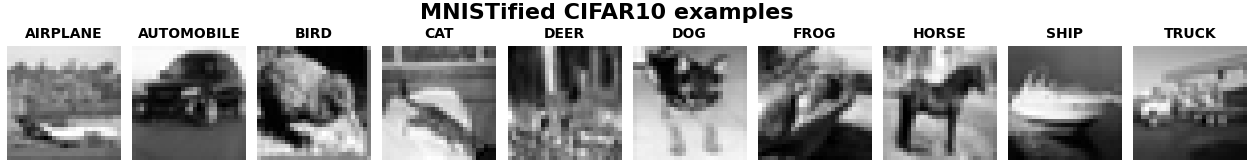
\includegraphics[width=0.99\textwidth]{Figures/Results/mnistified_cifar10.png}
\caption{Examples of the MNISTified CIFAR-10 dataset, where the RGB (three channel) images are converted to grayscale (single channel).}
\label{fig:mnistified_cifar10}
\end{figure}

For regression and classification models, the steering angle is appended as a suffix between the filename timestamp and the file extension e.g. 20250514\_154417\_678492\_steering\_0.0137.jpg where the minimum and maximum steering angles in software are -1 and 1, corresponding to -70 and +70 degrees in the simulator. By proportion we have 0.0137 equates to approximately 1 degree (0.959). The quantized steering angle label datasets (15, 5 and 3 bins) have corresponding values e.g. for a 5 bin quantized dataset (discreate values are -0.065, -0.015, 0.0000, 0.0150 and 0.0650) a typical image example from dataset carla\_dataset\_640x480\_06  is 20250523\_224719\_425145\_steering\_0.0150.jpg where the steering angle label is 0.0150 corresponding to 1.05 degrees. The maximum -0.065 and 0.065 correspond to -+4.55, which is sufficient steering to negociate the figure of eight circuit in CARLA's Town04 map. Datasets 12 and 13 (segmented 3 bin quantization, unbalanced and balanced) were extended  into datasets 14 and 15 to include a query e.g.
\begin{verbatim}
# ~/git/neurips-2025/scripts/train_carla_vlm_grok.py
# --- 2. Define System Message and Data Formatting ---
system_message = """You are a Vision Language Model specialized in steering 
vehicles.
Your task is to decide if the vehicle should turn left, turn right, or go 
straight based on the provided image and text description.
You should reply with only one of the following:
"Left", "Right", or "Straight".
(...)    
\end{verbatim}

and the labels -0.065, 0 and 0.065 were described in natural language as Left, Straight and Right. A Qwen (\cite{bai2023qwen}) (Qwen2-VL-2B-Instruct) and a DeepSeek (\cite{zeng2024deepseek}) (deepseek-vl-1.3b-chat) models consumed the Img+Q+L balanced and unbalanced datasets (Ids 14 and 15). Dataset Ids 16 and 17 were tested with a meta-llama (\cite{meta2024llama3vision}) (Llama-3.2-11B-Vision-Instruct) vision language model (VLM).


% 1200000
% 50000
% 550
% 2860
% 29105
% 29108
% 29105
% 29103
% 152996
% 27114
% 79206
% 26954
% 67391
% 26950
% 67380
% 50000
% 50000
% 1917822



% Table (alphabelical order
% Total examples: CIFAR-10 (50,000), MNIST (60,000), MNISTified English Handwritten Digits (550), MNISTified English Handwritten Alphabetical Characters (2,860), MNISTified CIFAR-10 (50,000).}

% table, quantity, description
% PMNIST, 1.2M, Perturbed MNIST
% MNISTified CIFAR-10, 50k, Grayscale CIFAR-10
% MNISTified English Handwritten Digits, 550
% MNISTified English Handwritten Characters, 2,860
% Directory: carla_dataset_640x480_01 - File Count: 29105, segmented with fiducials
% Directory: carla_dataset_640x480_02 - File Count: 29108, segmented
% Directory: carla_dataset_640x480_03 - File Count: 29105, fiducials only
% Directory: carla_dataset_640x480_05 - File Count: 29013, segmented 15 bins
% Directory: carla_dataset_640x480_05_balanced - File Count: 152996, segmented 15 bins balanced
% Directory: carla_dataset_640x480_06 - File Count: 27114 - segmented, 5 bins
% Directory: carla_dataset_640x480_06_balanced - File Count: 79206, segmented 5 bins
% Directory: carla_dataset_640x480_07_3_bins - File Count: 26954, segmented 3 bins
% Directory: carla_dataset_640x480_07_3_bins_balanced - File Count: 67391, segmented 3 bins balanced
% Directory: carla_dataset_640x480_07_3_bins_qwen - File Count: 26950, segmented 3 bin image/query/label
% Directory: carla_dataset_640x480_07_3_bins_qwen_balanced - File Count: 67380, segmented 3 bin image/query/label
% Directory: carla_dataset_640x480_segmented_with_fiducials - File Count: 28980, segmented with fiducials repeat

% Additionally 2 CIFAR-10 sets was created on-the-fly for the meta-llama/Llama-3.2-11B-Vision-Instruct zero-shot CIFAR-10 classification, 1440x1440 pixels (50k images) and 720x720 pixels (50k Images), in addition to the default 36x36 pixels CIFAR-10. Both additional resolutions were not written to disk.

% eog ~/git/neurips-2025/scripts/carla_dataset_640x480_01/20250513_192139_819274_steering_0.0000.jpg
% eog ~/git/neurips-2025/scripts/carla_dataset_640x480_02/20250514_153353_653641_steering_0.0000.jpg
% eog ~/git/neurips-2025/scripts/carla_dataset_640x480_03/20250514_195909_280821_steering_0.0000.jpg


\subsection{Noisy MNIST}

In this section we describe the Noisy MNIST dataset and related results

\subsection{MNISTified datasets}

% MNIStified CIFAR-10, from https://www.overleaf.com/project/67fab2a313a039351c852479 LOD-2025-wip
\begin{figure}[h]
\centering
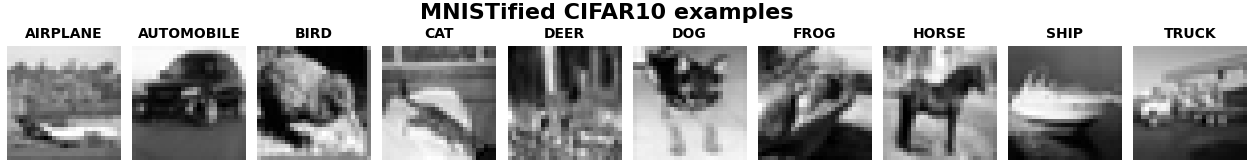
\includegraphics[width=0.99\textwidth]{Figures/Results/mnistified_cifar10.png}
\caption{Examples from the MNISTified CIFAR-10 dataset, where a sample of image classes are converted from RGB to grayscale}
\label{fig:mnistified_cifar10}
\end{figure}


\section{Training Quantized Models}

\subsection{Create datasets}

Discussion on the "Figure of 8" track.

\subsection{Training}





% \begin{figure}[h]
% \centering
% 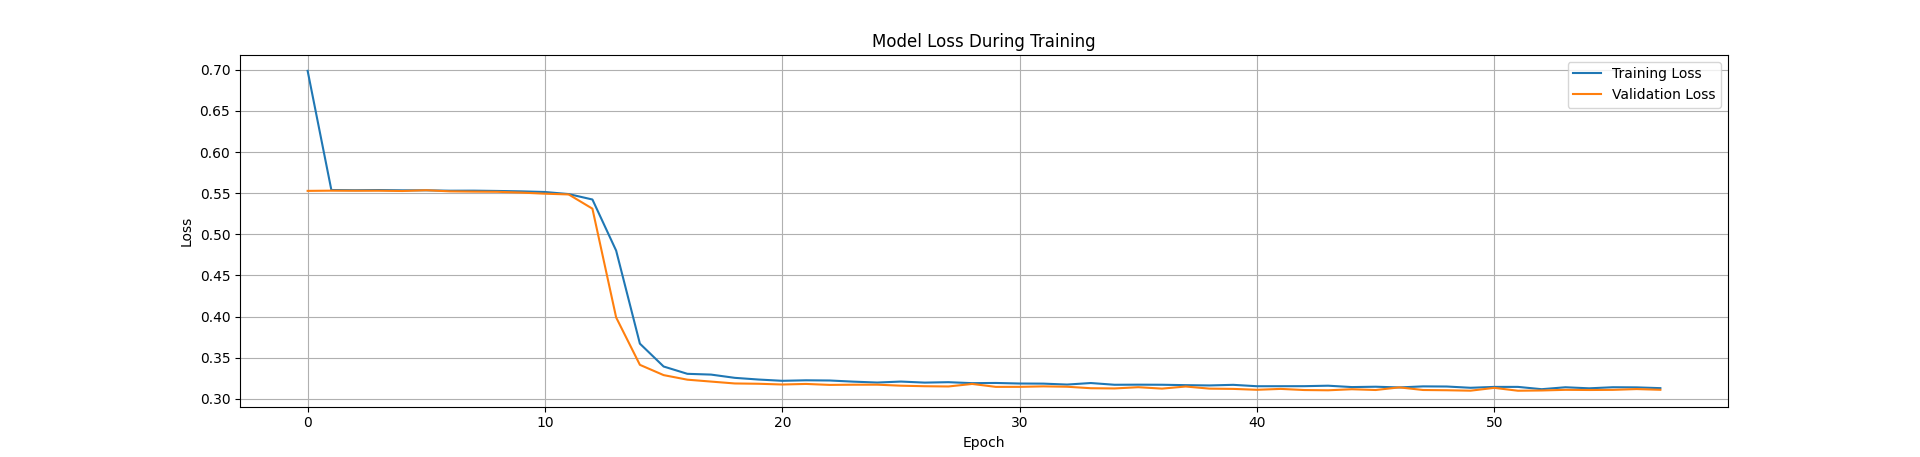
\includegraphics[width=0.2\textwidth]{Figures/Results/best_quantized_steering_model_3_bins_20250525-204246_model_loss_during_training.png}
% \caption{Model Loss During Training 5-bin dataset. The step-drop pattern is also observed with 15 and 3 bin datasets.}
% \label{fig:best_quantized_steering_model_3_bins_20250525-204246_model_loss_during_training}
% \end{figure}

% \begin{verbatim}
% Epoch [54/100], Train Loss: 0.3140, Val Loss: 0.3109, Train Acc: 86.93%, Val Acc: 87.06%
% Epoch 55/100:   0%|          | 0/337 [00:00<?, ?it/s]
% Epoch [55/100], Train Loss: 0.3127, Val Loss: 0.3107
% Epoch [55/100], Train Loss: 0.3127, Val Loss: 0.3107, Train Acc: 87.11%, Val Acc: 87.06%
% Epoch 56/100:   0%|          | 0/337 [00:00<?, ?it/s]
% Epoch [56/100], Train Loss: 0.3141, Val Loss: 0.3109
% Epoch [56/100], Train Loss: 0.3141, Val Loss: 0.3109, Train Acc: 87.01%, Val Acc: 87.01%
% Epoch 57/100:   0%|          | 0/337 [00:00<?, ?it/s]
% Epoch [57/100], Train Loss: 0.3139, Val Loss: 0.3118
% Epoch [57/100], Train Loss: 0.3139, Val Loss: 0.3118, Train Acc: 87.06%, Val Acc: 87.08%
% Epoch 58/100:   0%|          | 0/337 [00:00<?, ?it/s]
% Epoch [58/100], Train Loss: 0.3129, Val Loss: 0.3110
% Epoch [58/100], Train Loss: 0.3129, Val Loss: 0.3110, Train Acc: 86.97%, Val Acc: 87.14%
% Early stopping triggered
% Loading best model from best_quantized_steering_model_3_bins_20250525-204246.pth
% Training ended at: 2025-05-25 22:46:15
% Total execution time: 2:03:29.145624

% Epoch [39/100], Train Loss: 0.1990, Val Loss: 0.1960, Train Acc: 92.91%, Val Acc: 92.94%
% Epoch 40/100:   0%|          | 0/338 [00:00<?, ?it/s]
% Epoch [40/100], Train Loss: 0.1994, Val Loss: 0.1934
% Epoch [40/100], Train Loss: 0.1994, Val Loss: 0.1934, Train Acc: 93.08%, Val Acc: 92.90%
% Epoch 41/100:   0%|          | 0/338 [00:00<?, ?it/s]
% Epoch [41/100], Train Loss: 0.1995, Val Loss: 0.1928
% Epoch [41/100], Train Loss: 0.1995, Val Loss: 0.1928, Train Acc: 92.86%, Val Acc: 92.90%
% Epoch 42/100:   0%|          | 0/338 [00:00<?, ?it/s]
% Epoch [42/100], Train Loss: 0.1993, Val Loss: 0.1928
% Epoch [42/100], Train Loss: 0.1993, Val Loss: 0.1928, Train Acc: 92.87%, Val Acc: 93.03%
% Early stopping triggered
% Loading best model from best_quantized_steering_model_5_bins_20250525-204108.pth
% Training ended at: 2025-05-25 22:18:14
% Total execution time: 1:37:06.201752
    
% \end{verbatim}

% \subsection{Centroids}
% With unbalanced 15, 5 and 3 bin datasets:
% \begin{verbatim}
% Experiment 190
% python 14-generate-centroids.py \
%     --filename /home/daniel/git/neurips-2025/scripts/carla_dataset_640x480_05/15_bin_softmax_outputs.npy\
%     --bins 15

% Warning: No correct predictions for class 0. Centroid set to zeros.
% Warning: No correct predictions for class 1. Centroid set to zeros.
% Warning: No correct predictions for class 2. Centroid set to zeros.
% Warning: No correct predictions for class 8. Centroid set to zeros.
% Warning: No correct predictions for class 11. Centroid set to zeros.
% Warning: No correct predictions for class 12. Centroid set to zeros.
% Warning: No correct predictions for class 13. Centroid set to zeros.
% Saved centroids to /home/daniel/git/neurips-2025/scripts/carla_dataset_640x480_05/15_bins_centroids.npy

% # 5 bins
% python 14-generate-centroids.py \
%     --filename /home/daniel/git/neurips-2025/scripts/carla_dataset_640x480_06/5_bin_softmax_outputs.npy\
%     --bins 5

% Saved centroids to /home/daniel/git/neurips-2025/scripts/carla_dataset_640x480_06/5_bins_centroids.npy
% Centroids for 5 bins:
% Class 0: [5.93501530e-01 4.01932724e-01 4.21476976e-03 3.06535164e-04
%  4.44427381e-05]
% Class 1: [3.48384826e-02 8.40230296e-01 1.24839201e-01 6.73436989e-05
%  2.46761301e-05]
% Class 2: [1.34825375e-04 6.20000780e-03 9.86949412e-01 6.68143048e-03
%  3.43238712e-05]
% Class 3: [5.93253221e-05 1.21105444e-07 5.55497731e-03 9.12405940e-01
%  8.19796364e-02]
% Class 4: [2.31054104e-05 2.15194062e-14 4.34885197e-08 1.16364635e-01
%  8.83612225e-01]
 
% # 3 bins
% python 14-generate-centroids.py \
%     --filename /home/daniel/git/neurips-2025/scripts/carla_dataset_640x480_07_3_bins/3_bin_softmax_outputs.npy\
%     --bins 3
% Saved centroids to /home/daniel/git/neurips-2025/scripts/carla_dataset_640x480_07_3_bins/3_bins_centroids.npy
% Centroids for 3 bins:
% Class 0: [5.95680285e-01 4.04128073e-01 1.91640343e-04]
% Class 1: [0.03206146 0.90113858 0.06679997]
% Class 2: [3.11515402e-06 2.61644563e-01 7.38352321e-01]

% Conclusion, not as closely separated as MNIST and CIFAR.
% Action, train on balanced datasets.

% \end{verbatim}
% With balanced 15, 5 and 3 bin datasets:
% \begin{verbatim}
    
% \end{verbatim}

%%%%%%%%%%%%%%%%%%%%%%%%%%%%%%%%%%%%%%
% BALANCING 15, 5 and 3 BIN DATASETS %
%%%%%%%%%%%%%%%%%%%%%%%%%%%%%%%%%%%%%%

\subsection{Balancing the 15, 5 and 3 bin datasets}
Discussion to be added, how images of minority class were duplicated to match size of majority class.

%%%%%%%%%%%%%%%%%%%%%%%%%%%%%%%%%%%%%%%%%%%%%%%%%%%%%%%
% TRAINING CNN WITH 15, 5 and 3 BIN BALANCED DATASETS %
%%%%%%%%%%%%%%%%%%%%%%%%%%%%%%%%%%%%%%%%%%%%%%%%%%%%%%%

\section{Training with balanced dataset}

\begin{figure}[h]
\centering
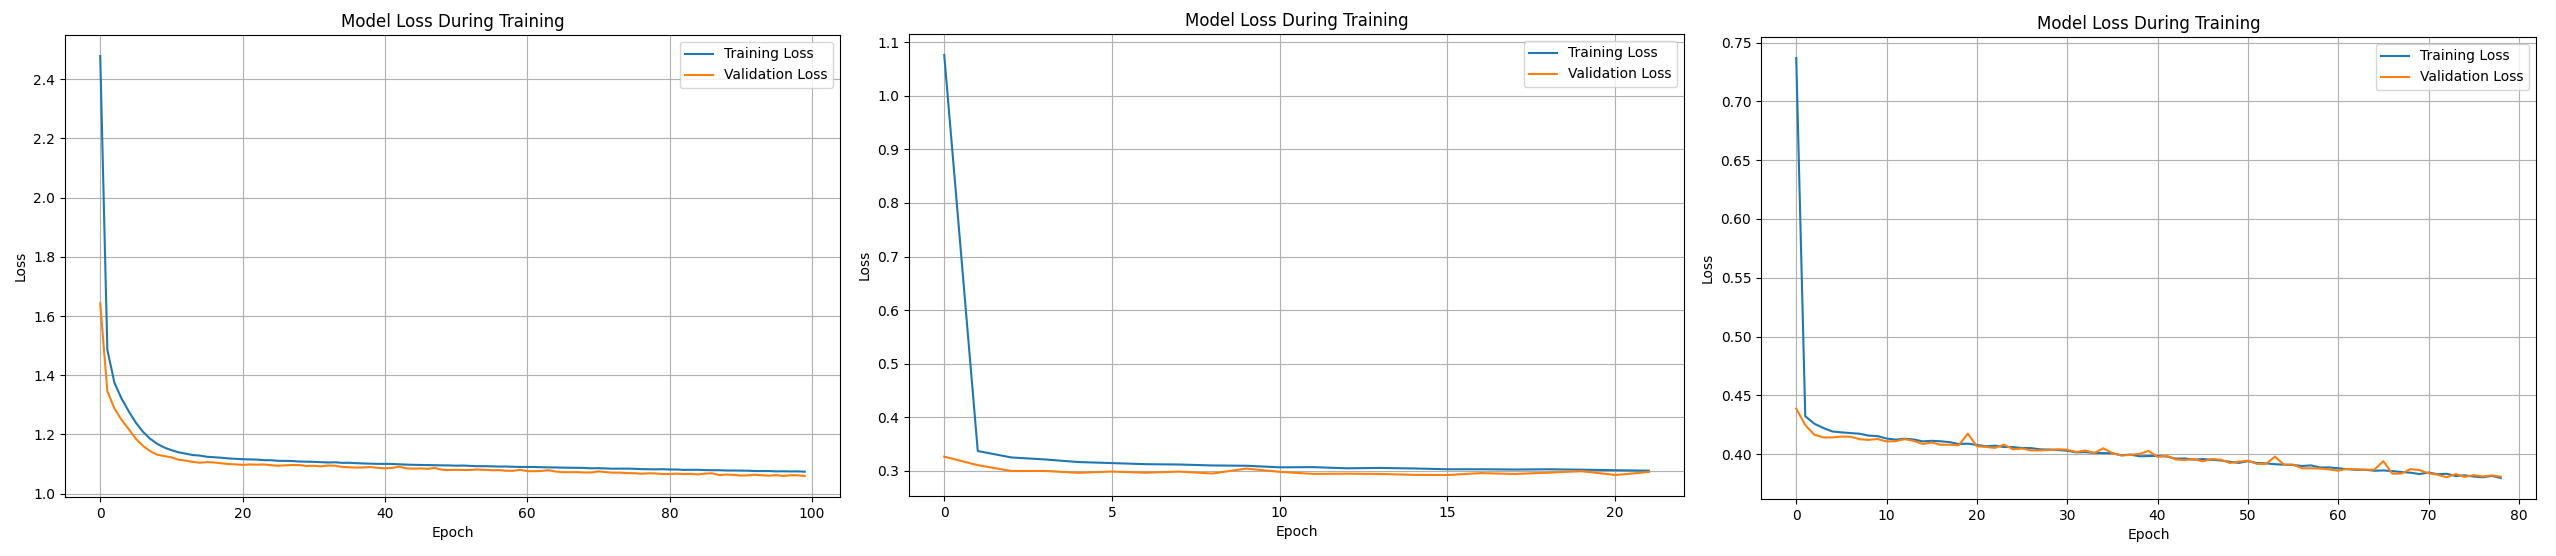
\includegraphics[width=0.99\textwidth]{Figures/Results/CNN_15_5_3_balanced_training.png}
\caption{Model Training and Evaluation Loss, from left to right, 15, 5 and 3-bin Classifier CNNs trained on balanced dataset.}
\label{fig:CNN_15_5_3_balanced_training}
\end{figure}

Figure~\ref{fig:CNN_15_5_3_balanced_training} presents training and validation loss curves for CNN classifiers trained on balanced datasets with 15, 5, and 3 quantized steering angle bins, shown left to right. The total number of samples for each dataset was approximately 153,000 (15-bin), 79,000 (5-bin), and 67,000 (3-bin).

The 15-bin model trained for the full 100 epochs without early stopping. Final training and validation losses were approximately 1.07 and 1.06, respectively, with accuracies around 48\%.

The 5-bin model triggered early stopping at epoch 22. Final losses were approximately 0.30 (training) and 0.30 (validation), with training and validation accuracies near 87\%.

The 3-bin model triggered early stopping at epoch 79. Final losses were approximately 0.38 (training) and 0.38 (validation), with accuracies near 83\%.

Training durations were approximately 18 hours (15-bin), 2.5 hours (5-bin), and 6.9 hours (3-bin). Dataset size differences correspond to variations in training duration and number of training iterations.

%%%%%%%%%
% PLOTS %
%%%%%%%%%

%%%%%%%%%%%%%%%%%%
% 15 BIN DATASET %
%%%%%%%%%%%%%%%%%%



% \begin{figure}[H]
% \centering
% 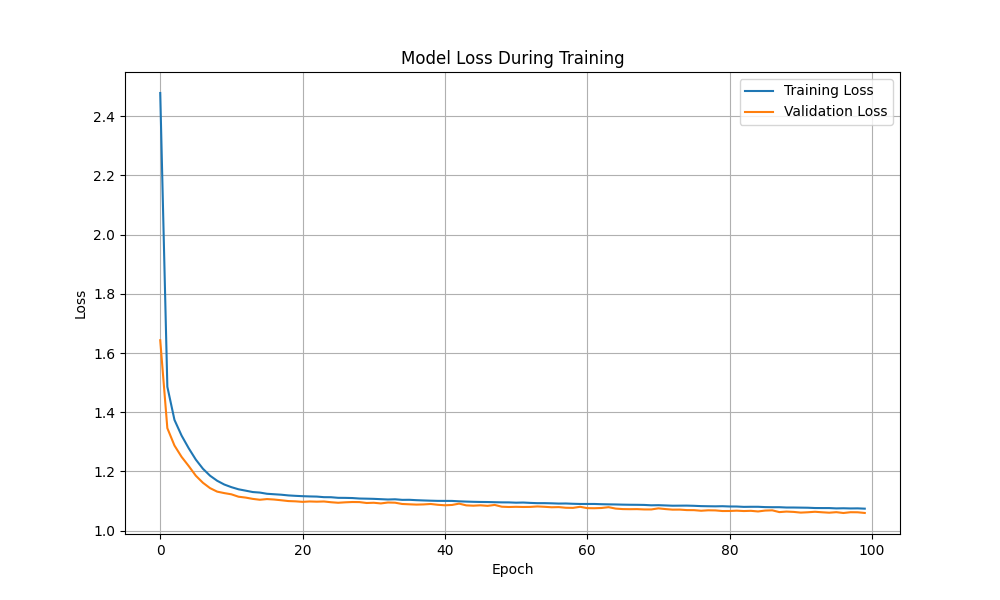
\includegraphics[width=1\linewidth]{Figures/Results/best_quantized_steering_model_15_bins_balanced_20250529-211117.pth_training.png}
% \caption{15-bin balanced dataset training}
% \label{fig:best_quantized_steering_model_15_bins_balanced_20250529-211117.pth_training}
% \end{figure}

% \begin{verbatim}

% (carla-env) daniel@simbox ~/git/neurips-2025/scripts (master)$ ^C
% (carla-env) daniel@simbox ~/git/neurips-2025/scripts (master)$ python 07-training-from-config_05_15_bin_balanced.py
% Total number of samples: 152985
% Training samples: 122388, Validation samples: 30597
% Batch image shape: torch.Size([64, 3, 66, 200])
% Batch class indices shape: torch.Size([64])
% Training started at: 2025-05-29 21:11:17
% Epoch 1/100:   0%|          | 0/1913 [00:00<?, ?it/s]
% Epoch [1/100], Train Loss: 2.4783, Val Loss: 1.6433
% Epoch [1/100], Train Loss: 2.4783, Val Loss: 1.6433, Train Acc: 14.54%, Val Acc: 38.12%
% (...)
% Epoch [97/100], Train Loss: 1.0757, Val Loss: 1.0597, Train Acc: 47.79%, Val Acc: 48.01%
% New best model! Saving to best_quantized_steering_model_15_bins_balanced_20250529-211117.pth
% Epoch 98/100:   0%|          | 0/1913 [00:00<?, ?it/s]
% Epoch [98/100], Train Loss: 1.0751, Val Loss: 1.0624
% Epoch [98/100], Train Loss: 1.0751, Val Loss: 1.0624, Train Acc: 47.79%, Val Acc: 47.71%
% Epoch 99/100:   0%|          | 0/1913 [00:00<?, ?it/s]
% Epoch [99/100], Train Loss: 1.0754, Val Loss: 1.0621
% Epoch [99/100], Train Loss: 1.0754, Val Loss: 1.0621, Train Acc: 47.80%, Val Acc: 49.28%
% Epoch 100/100:   0%|          | 0/1913 [00:00<?, ?it/s]
% Epoch [100/100], Train Loss: 1.0744, Val Loss: 1.0598
% Epoch [100/100], Train Loss: 1.0744, Val Loss: 1.0598, Train Acc: 48.01%, Val Acc: 47.81%
% Training ended at: 2025-05-30 15:02:31
% Total execution time: 17:51:13.434644

% \end{verbatim}

%%%%%%%%%%%%%%%%%
% 5 BIN DATASET %
%%%%%%%%%%%%%%%%%

% \begin{figure}[H]
% \centering
% 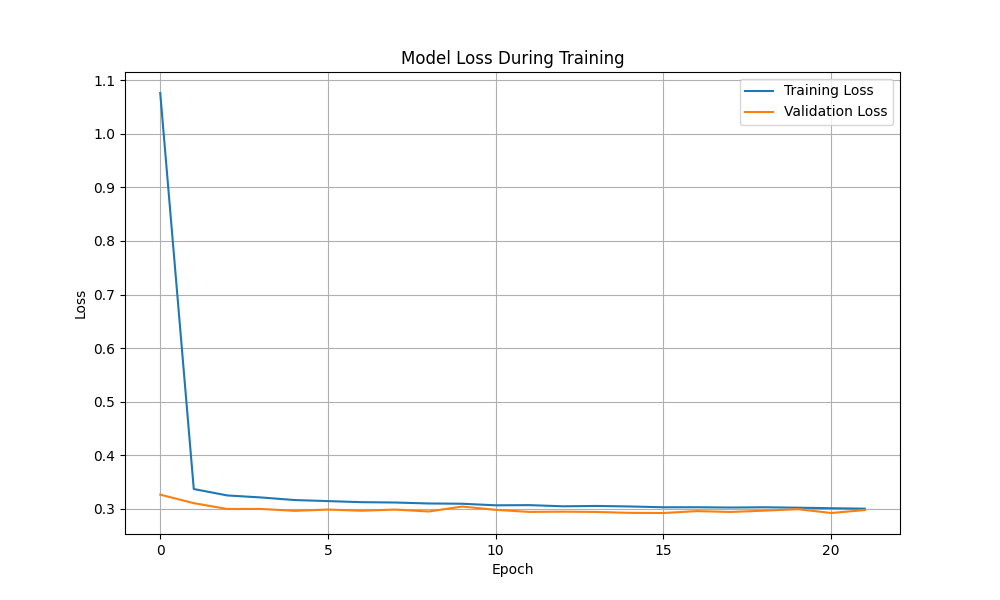
\includegraphics[width=1\linewidth]{Figures/Results/best_quantized_steering_model_5_bins_balanced_20250529-211142.pth_training.png}
% \caption{Loss plot for CNN training on 5-bin balanced dataset}
% \label{fig:best_quantized_steering_model_5_bins_balanced_20250529-211142.pth_training}
% \end{figure}

% \begin{verbatim}
% (carla-env) daniel@simbox ~/git/neurips-2025/scripts (master)$ python 07-training-from-config_07_3_bins_balanced.py
% Total number of samples: 67380
% Training samples: 53904, Validation samples: 13476
% Batch image shape: torch.Size([64, 3, 66, 200])
% Batch class indices shape: torch.Size([64])
% Training started at: 2025-05-29 21:24:49

% Epoch [78/100], Train Loss: 0.3815, Val Loss: 0.3819, Train Acc: 83.00%, Val Acc: 82.70%
% Epoch 79/100:   0%|          | 0/843 [00:00<?, ?it/s]
% Epoch [79/100], Train Loss: 0.3797, Val Loss: 0.3808
% Epoch [79/100], Train Loss: 0.3797, Val Loss: 0.3808, Train Acc: 83.16%, Val Acc: 83.02%
% Early stopping triggered
% Loading best model from best_quantized_steering_model_3_bins_balanced_20250529-212449.pth
% Training ended at: 2025-05-30 04:20:09
% Total execution time: 6:55:19.815357

% \end{verbatim}

%%%%%%%%%%%%%%%%%
% 3 BIN DATASET %
%%%%%%%%%%%%%%%%%

% \begin{figure}[H]
% \centering
% 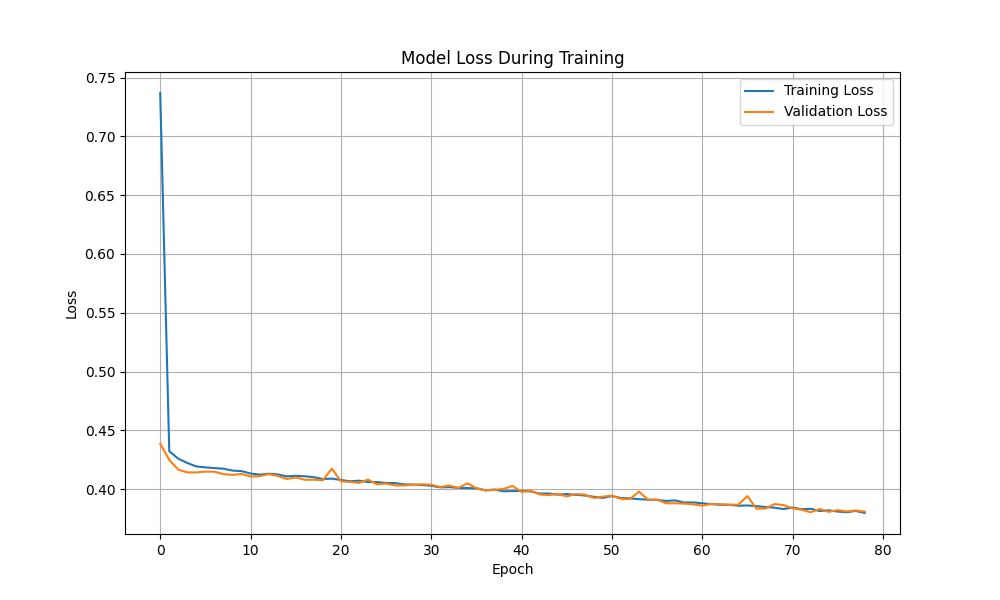
\includegraphics[width=1\linewidth]{Figures/Results/best_quantized_steering_model_3_bins_balanced_20250529-212449.pth_training.png}
% \caption{3-bin balanced dataset training}
% \label{fig:best_quantized_steering_model_3_bins_balanced_20250529-212449.pth_training}
% \end{figure}

% \begin{verbatim}
% (carla-env) daniel@simbox ~/git/neurips-2025/scripts (master)$ python 07-training-from-config_06_5_bins_balanced.py
% Total number of samples: 79195
% Training samples: 63356, Validation samples: 15839
% Batch image shape: torch.Size([64, 3, 66, 200])
% Batch class indices shape: torch.Size([64])
% Training started at: 2025-05-29 21:11:42

% Epoch [21/100], Train Loss: 0.3009, Val Loss: 0.2920, Train Acc: 87.56%, Val Acc: 87.48%
% Epoch 22/100:   0%|          | 0/990 [00:00<?, ?it/s]
% Epoch [22/100], Train Loss: 0.3001, Val Loss: 0.2975
% Epoch [22/100], Train Loss: 0.3001, Val Loss: 0.2975, Train Acc: 87.45%, Val Acc: 86.92%
% Early stopping triggered
% Loading best model from best_quantized_steering_model_5_bins_balanced_20250529-211142.pth
% Training ended at: 2025-05-29 23:41:51
% Total execution time: 2:30:08.752455

% \end{verbatim}

%%%%%%%%%%%%%%%%%%%%%%%%%%%%%%%%%%%%%%%%%%%%%%%%%
% TRAINING AND INFERENCE RESULTS FOR REGRESSION %
% AND CLASSIFICATION MODELS                     %
%%%%%%%%%%%%%%%%%%%%%%%%%%%%%%%%%%%%%%%%%%%%%%%%%

\section{Training and Inference Results for Regression and Classification Models}

We first trained regression models on datasets labeled with continuous steering values, corresponding to steering angles in the range -70 to 70 degrees, mapping to -1 to 1 steering units in CARLA simulator code. The trained models were evaluated in inference mode by allowing them to autonomously drive around the Town04 figure-of-eight circuit. During these runs, no lane invasions were observed; that is, the lateral deviation from the planned path, measured by the D MAE metric, remained below the defined threshold of 0.85 units. Following the procedure described in Section~\ref{methods:regression_classification}, these regression models were then adapted into classifiers by quantizing the continuous steering labels into discrete bins. The results for both the regression and classification models, during training and inference, are presented in the following sections.

%%%%%%%%%%%%%%%%%%%%%
% REGRESSION MODELS %
%%%%%%%%%%%%%%%%%%%%%

\subsection{Regression Models}
\begin{longtable}{@{}lllllll@{}}
\toprule
Model Name & Dataset & Train Loss & Eval Loss & MAE & O MAE & D MAE \\
\midrule
\endfirsthead
\toprule
Model Name & Dataset & Train Loss & Eval Loss & MAE & O MAE & D MAE \\
\midrule
\endhead
RegCNNCUFid & Cont Unbal w/ Fids & 0.0000 & 0.0000 & N/A & 0.0036 & 0.0461 \\
RegCNNCU & Continuous Unbal & N/A & N/A & N/A & 0.0033 & 0.0588 \\
RgrViTCU & Continuous Unbal & 0.0002 & 0.0001 & 0.0076 & 0.0076 & 0.0399 \\
\bottomrule
\caption{Regression Model Performance}
\label{results:table_regression_models}
\end{longtable}

Table~\ref{results:table_regression_models} reports the performance of three regression models trained on the continuous unbalanced dataset. The columns are as follows: Train Loss and Eval Loss refer to the mean squared error on the training and evaluation sets, respectively; MAE is the mean absolute error computed during training; O MAE is the mean absolute error calculated over the combined training and evaluation sets; and D MAE is the mean absolute lateral deviation of the simulated vehicle from the centerline, measured during autonomous driving in the Town04 figure-of-eight loop. Where N/A appears, the corresponding value was not recorded during training.

The RegCNNCUFid model incorporates fiducial markers as input and achieved a D MAE of 0.0461, with an O MAE of 0.0036. The RegCNNCU model, which uses the same architecture without fiducials, obtained a slightly lower O MAE (0.0033) but a higher D MAE (0.0588). The difference in D MAE between these two models is small and may be attributed to statistical noise, as both values remain well below the operational threshold of 0.85, beyond which lane invasion would occur.

The RgrViTCU model, based on a ViT architecture, yielded an O MAE of 0.0076 and the lowest D MAE among the three (0.0399). Since MAE values were not recorded for the CNN-based models, comparisons across all models using that column are not possible. All D MAE values are within the bounds of acceptable simulated driving behavior, and the differences observed do not approach the threshold of operational relevance.

% Code ~/git/neurips-2025/scripts/16-save-report-results.py
% T Acc and V Acc not agreeing with O Acc for CNN classifiers.
% I did a spot check for ClsCNN15bB and the figures for T Acc and V Acc 
% (experiment 192 - training) and T Acc (Experiment 223 - evaluation) are correctly
% copied from reported results.
% Model generated by training is 

% Found one possible issue - bottom was cropped at 400
    % # --- CRITICAL FIX: MATCH TRAINING SCRIPT'S CROPPING ---
    % crop_top = 210    # Original: 200
    % crop_bottom = 480 # Original: 400
    % resize_width = 200
    % resize_height = 66

%%%%%%%%%%%%%%%%%%%%%%%%%
% CLASSIFICATION MODELS %
%%%%%%%%%%%%%%%%%%%%%%%%%

\subsection{Classification Models}
% \begin{longtable}{@{}llllllll@{}}
% \toprule
% Model Name & Dataset & T Acc & T Loss & V Acc & V Loss & O Acc & D MAE \\
% \midrule
% \endfirsthead
% \toprule
% Model Name & Dataset & T Acc & T Loss & V Acc & V Loss & O Acc & D MAE \\
% \midrule
% \endhead
% ClsCNN3bB & 3-bin Bal & 83.16\% & 0.3797 & 83.02\% & 0.3808 & 53.78\% & 0.0365 \\
% ClsCNN3bU & 3-bin Unbal & 86.97\% & 0.3129 & 87.14\% & 0.3110 & 85.15\% & 0.0466 \\
% ClsCNN5bB & 5-bin Bal & 87.45\% & 0.3001 & 86.92\% & 0.2975 & 83.79\% & 0.0491 \\
% ClsCNN5bU & 5-bin Unbal & 92.87\% & 0.1993 & 93.03\% & 0.1928 & 92.71\% & 0.0753 \\
% ClsCNN15bB & 15-bin Bal & 48.01\% & 1.0744 & 47.81\% & 1.0598 & 32.58\% & 0.0162 \\
% ClsCNN15bU & 15-bin Unbal & 73.76\% & 0.7241 & 75.34\% & 0.6839 & 56.09\% & 0.0194 \\
% ClsViT3bB & 3-bin Bal & N/A & 0.1875 & 97.15\% & 0.0960 & 97.97\% & 0.0462 \\
% ClsViT3bU & 3-bin Unbal & N/A & 0.2625 & 91.93\% & 0.2075 & 92.50\% & 0.0397 \\
% ClsViT5bB & 5-bin Bal & N/A & 0.1317 & 97.54\% & 0.0766 & 97.77\% & 0.0454 \\
% ClsViT5bU & 5-bin Unbal & N/A & 0.1985 & 94.05\% & 0.1590 & 94.97\% & 0.0666 \\
% ClsViT15bB & 15-bin Bal & N/A & 0.4012 & 92.92\% & 0.1984 & 93.86\% & 0.0925 \\
% ClsViT15bU & 15-bin Unbal & N/A & N/A & N/A & N/A & 76.55\% & 0.0844 \\
% \bottomrule
% \caption{Classification Model Performance: training and self-driving, with quantized balanced and unbalanced datasets. The first row shows data for a CNN classifier trained on a 3-bin dataset - steering angles -0.065 (-4.55 degrees), 0 and 0.065 (4.55 degrees). The training accuracy is 83.17\%, the training loss 0.3739, the validation accuracy 83.02\%, the validation loss 0.3808, the overall accuracy when training and validation datasets are combined is 53.78\%. The distance mean average error (DMAE)}
% \end{longtable}

\begin{longtable}{@{}llllllll@{}}
\toprule
Model Name & Dataset & T Acc & T Loss & V Acc & V Loss & O Acc & D MAE \\
\midrule
\endfirsthead
\toprule
Model Name & Dataset & T Acc & T Loss & V Acc & V Loss & O Acc & D MAE \\
\midrule
\endhead
ClsCNN3bB & 3-bin Bal & 83.16\% & 0.3797 & 83.02\% & 0.3808 & 83.36\% & 0.0365 \\
ClsCNN3bU & 3-bin Unbal & 86.97\% & 0.3129 & 87.14\% & 0.3110 & 87.36\% & 0.0466 \\
ClsCNN5bB & 5-bin Bal & 87.45\% & 0.3001 & 86.92\% & 0.2975 & 87.70\% & 0.0491 \\
ClsCNN5bU & 5-bin Unbal & 92.87\% & 0.1993 & 93.03\% & 0.1928 & 93.18\% & 0.0753 \\
ClsCNN15bB & 15-bin Bal & 48.01\% & 1.0744 & 47.81\% & 1.0598 & 48.01\% & 0.0162 \\
ClsCNN15bU & 15-bin Unbal & 73.76\% & 0.7241 & 75.34\% & 0.6839 & 75.11\% & 0.0194 \\
ClsViT3bB & 3-bin Bal & N/A & 0.1875 & 97.15\% & 0.0960 & 97.97\% & 0.0462 \\
ClsViT3bU & 3-bin Unbal & N/A & 0.2625 & 91.93\% & 0.2075 & 92.50\% & 0.0397 \\
ClsViT5bB & 5-bin Bal & N/A & 0.1317 & 97.54\% & 0.0766 & 97.77\% & 0.0454 \\
ClsViT5bU & 5-bin Unbal & N/A & 0.1985 & 94.05\% & 0.1590 & 94.97\% & 0.0666 \\
ClsViT15bB & 15-bin Bal & N/A & 0.4012 & 92.92\% & 0.1984 & 93.86\% & 0.0925 \\
ClsViT15bU & 15-bin Unbal & N/A & N/A & N/A & N/A & 76.55\% & 0.0844 \\
\bottomrule
\caption{Classification Model Performance: training and self-driving, with quantized balanced and unbalanced datasets. The first row shows data for a CNN classifier trained on a 3-bin dataset - steering angles -0.065 (-4.55 degrees), 0 and 0.065 (4.55 degrees). The training accuracy is 83.17\%, the training loss 0.3739, the validation accuracy 83.02\%, the validation loss 0.3808, the overall accuracy when training and validation datasets are combined is 83.36\%. The distance mean average error (DMAE)}
\label{results:classifier_models_results_table}
\end{longtable}

Table~\ref{results:classifier_models_results_table} presents the results for CNN and ViT models that were converted from regression models to perform classification, under three quantization schemes—3, 5, and 15 steering angle bins—and using either balanced or unbalanced datasets. The columns are as follows: T Acc and T Loss denote training accuracy and training loss; V Acc and V Loss are validation accuracy and validation loss; O Acc represents the overall accuracy across the full dataset (training and validation combined); and D MAE is the mean absolute error of the vehicle’s lateral deviation from the centerline. Entries marked N/A indicate that the corresponding values were not recorded during training. The D MAE values were computed through inference: after training, each model was deployed to drive autonomously around the Town04 figure-of-eight track, and its average distance from the intended trajectory was measured.

Among the CNN classifiers, ClsCNN5bU (trained on the unbalanced 5-bin dataset) achieved the highest overall accuracy (93.18\%), making it the best-performing CNN model. While its D MAE was slightly higher (0.0753), this remains well below the threshold (0.85 units) beyond which the vehicle would cross into an adjacent lane—meaning the deviation is not operationally significant and may be attributed to statistical noise. For the ViT models, ClsViT3bB (trained on the balanced 3-bin dataset) showed the strongest performance, with an overall accuracy of 97.97\% and a D MAE of 0.0462. In general, ViT models outperformed CNNs in both accuracy and driving precision, particularly on balanced datasets with coarser quantization. Given the low D MAE values across the board, most differences are unlikely to be practically significant in terms of simulated driving safety.

Overall Accuracy for CNN classifiers is consistenly higher for models trained on unbalanced datasets, while the trend is inverted for ViT classifiers. This may be related to dataset sizes and network capacity, and is set as an investigative topic for future work.

\subsection{Analysis of Classifier Outputs}

This section presents the results for the best performing models.

%%%%%%%%%%%%%%%%%%%%%%%%
% ClsCNN5binUnbalanced %
%%%%%%%%%%%%%%%%%%%%%%%%

\subsubsection{ClsCNN5binUnbalanced}

\begin{table}[htbp]
\centering
\begin{tabular}{@{}lcccc@{}}
\toprule
\textbf{Class} & \textbf{Precision} & \textbf{Recall} & \textbf{F1-Score} & \textbf{Support} \\
\midrule
$-0.065$ & 0.80 & 0.36 & 0.50 & 401 \\
$-0.015$ & 0.85 & 0.97 & 0.90 & 5,843 \\
$\phantom{-}0.000$ & 0.98 & 0.95 & 0.97 & 15,839 \\
$\phantom{-}0.015$ & 0.90 & 0.96 & 0.93 & 3,972 \\
$\phantom{-}0.065$ & 0.87 & 0.57 & 0.69 & 936 \\
\midrule
\textbf{Macro Avg} & \textbf{0.88} & \textbf{0.76} & \textbf{0.80} & \textbf{26,991} \\
\bottomrule
\end{tabular}
\caption{Classification performance results for the ClsCNN5binUnbalanced model. The model achieved an overall accuracy of 93.18\% with a mean confidence of 0.9294 across 26,991 test images.}
\label{tab:clf_report_ClsCNN5binUnbalanced}
\end{table}

\begin{figure}[H]
\centering
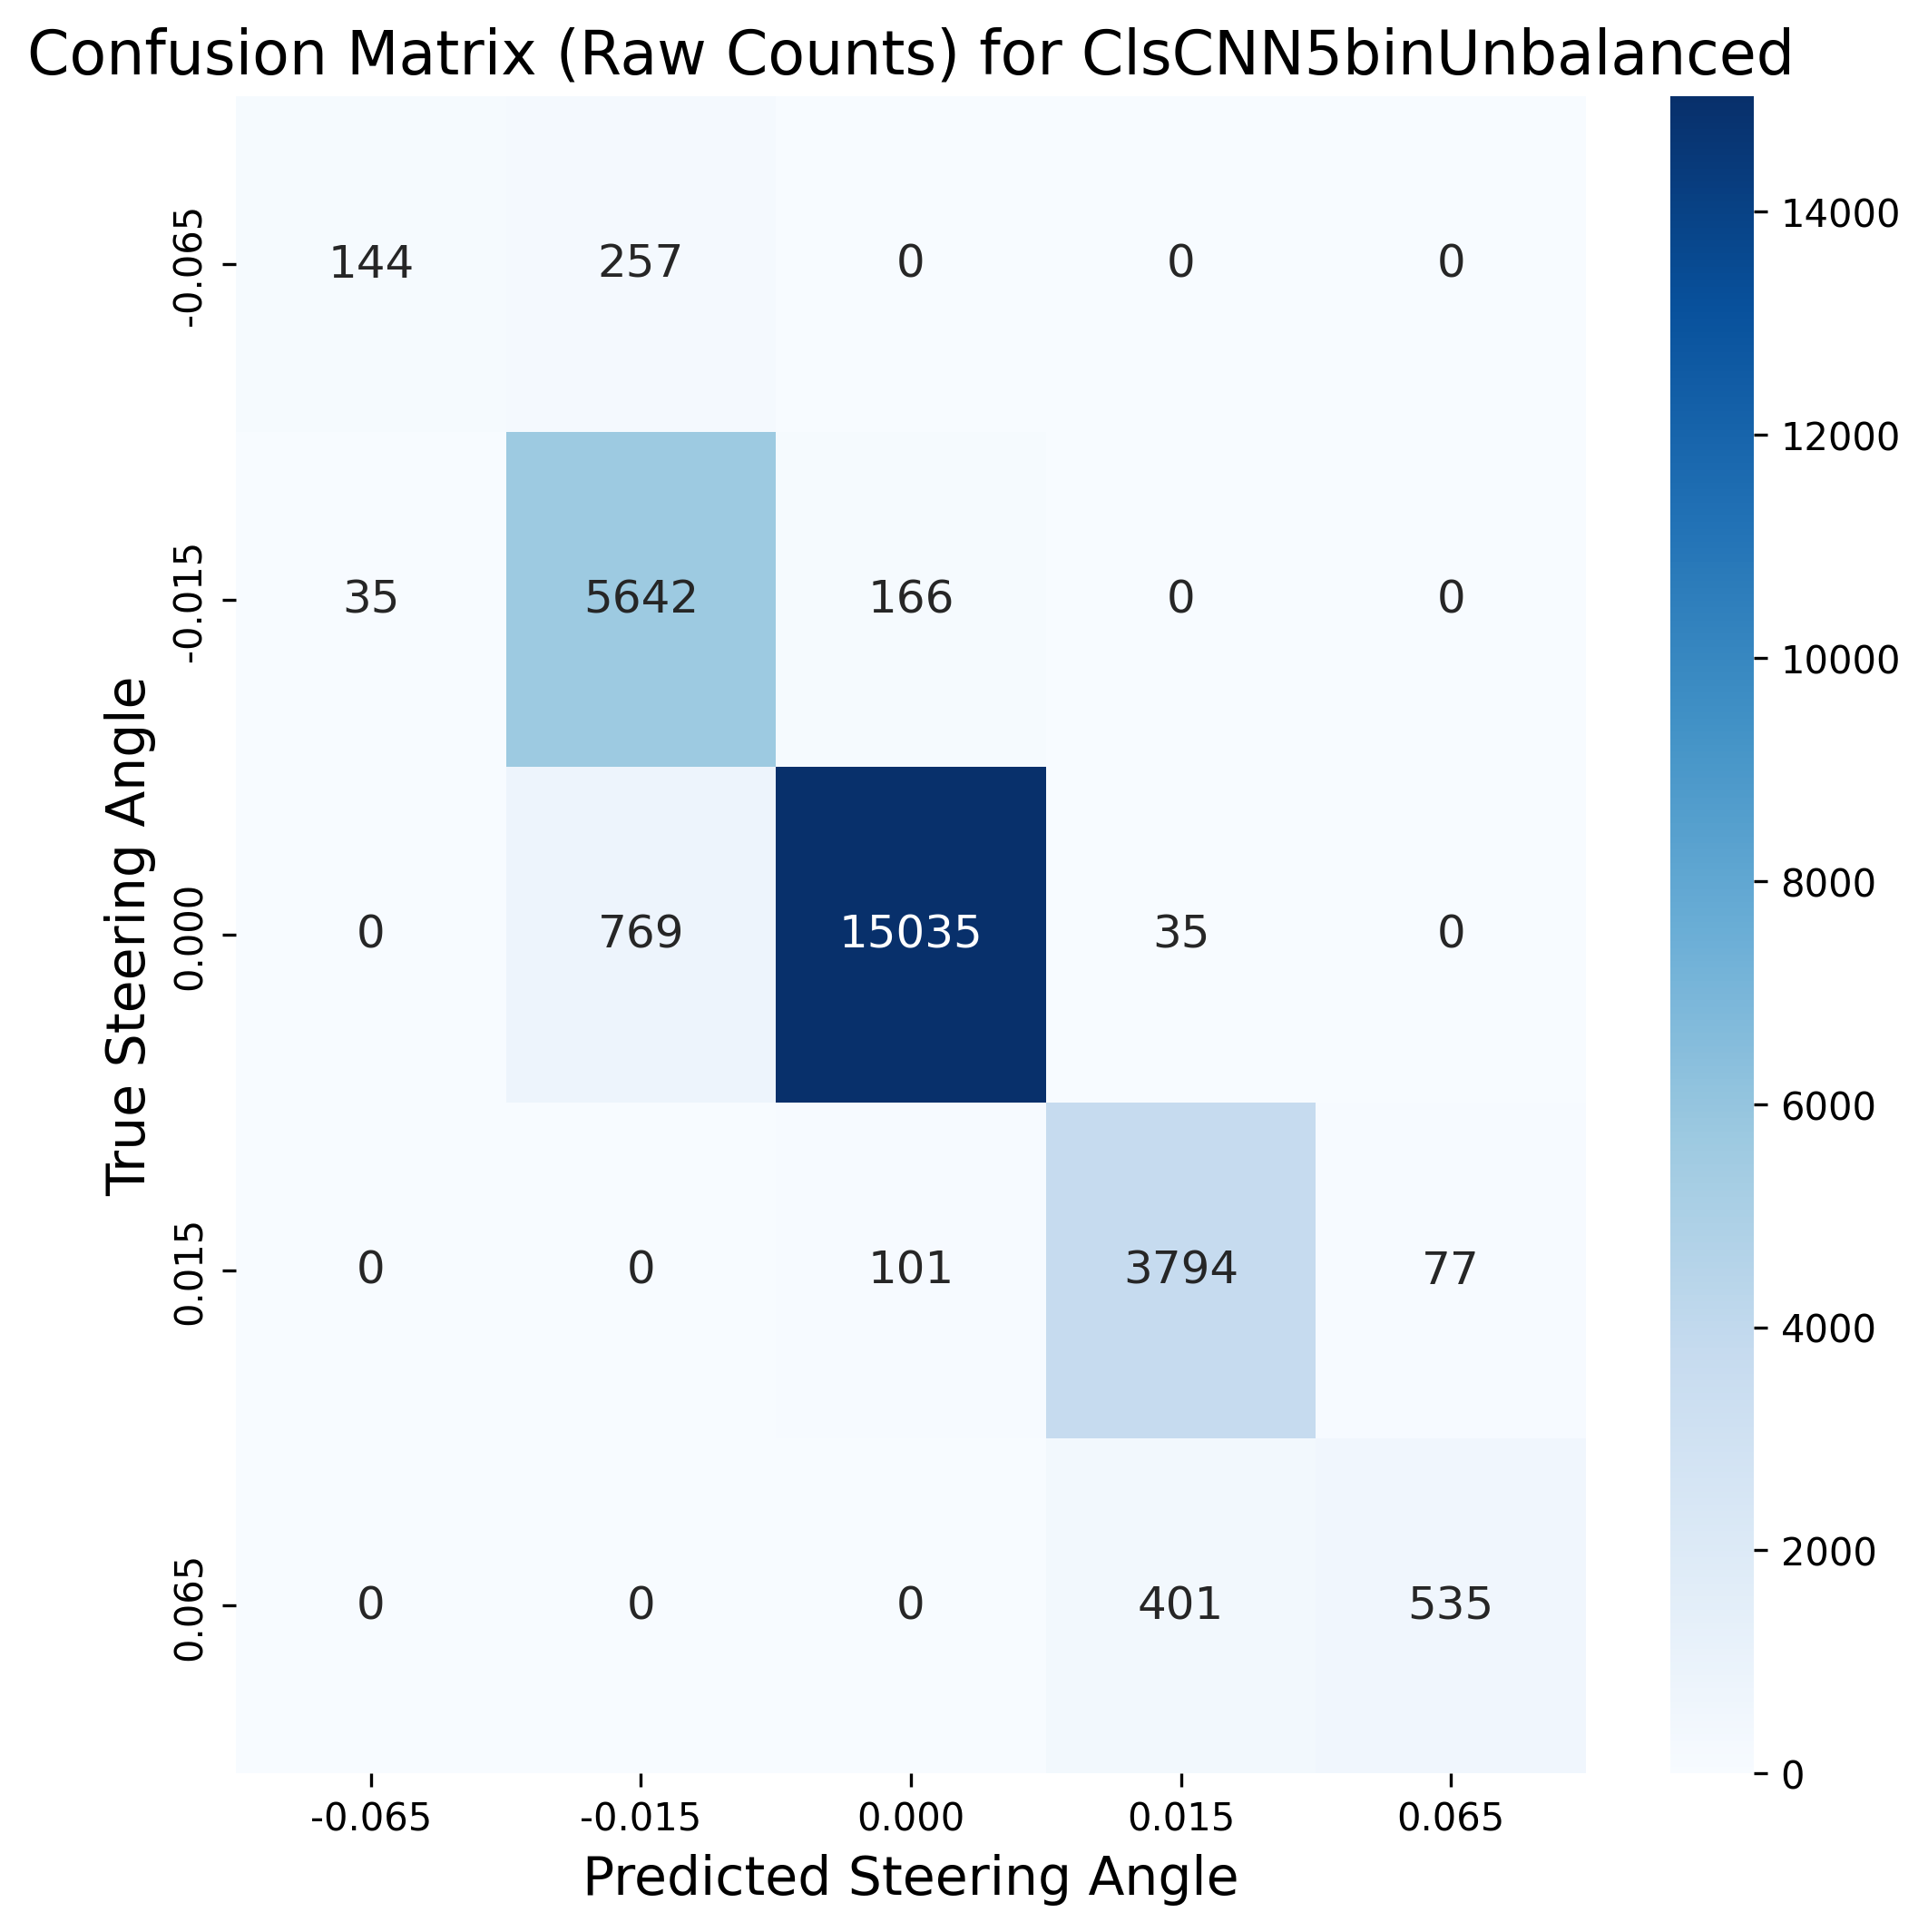
\includegraphics[width=0.65\linewidth]{Figures/Results/cm_raw_ClsCNN5binUnbalanced.png}
\caption{ClsCNN5binUnbalanced model raw counts confusion matrix}
\label{fig:cm_raw_ClsCNN5binUnbalanced}
\end{figure}

\begin{figure}[H]
    \centering
    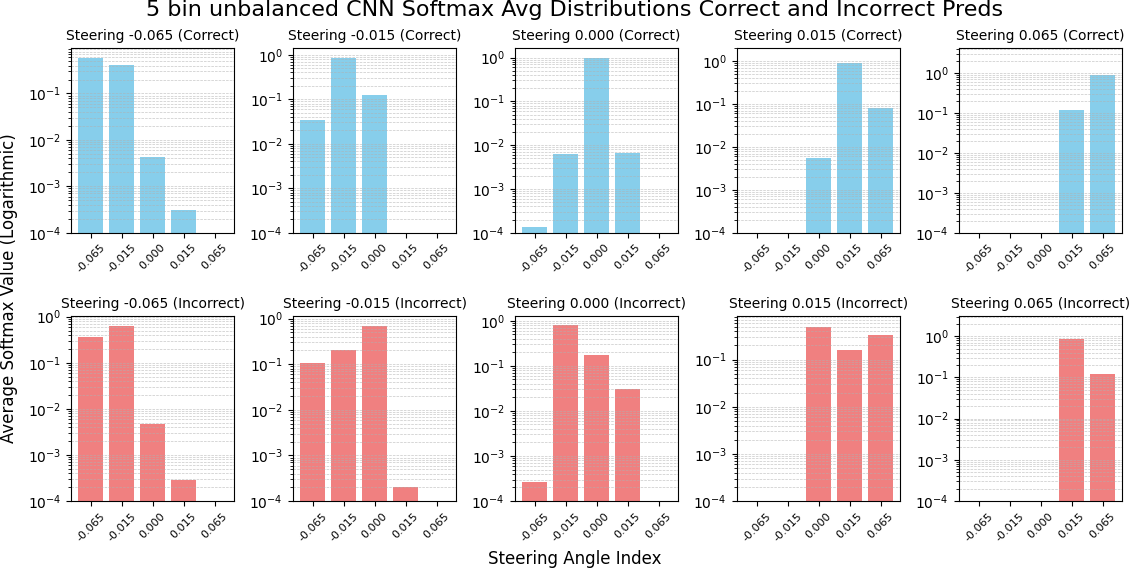
\includegraphics[width=1\linewidth]{Figures/Results/5_bins_cnn_softmax_dist_plot_unbalanced.png}
    \caption{Average Softmax Probabilities for Correctly and Incorrectly Classified Steering Angles in the 5 bin cnn unbalanced training Dataset.}
    \label{fig:5_bins_cnn_softmax_dist_unbalanced}
\end{figure}

%%%%%%%%%%%%%%%%%%%%%%
% ClsViT3binBalanced %
%%%%%%%%%%%%%%%%%%%%%%

\subsubsection{ClsViT3binBalanced}

\begin{table}[htbp]
\centering
\begin{tabular}{@{}lcccc@{}}
\toprule
\textbf{Class} & \textbf{Precision} & \textbf{Recall} & \textbf{F1-Score} & \textbf{Support} \\
\midrule
$-0.065$ & 0.98 & 1.00 & 0.99 & 22,460 \\
$\phantom{-}0.000$ & 1.00 & 0.94 & 0.97 & 22,460 \\
$\phantom{-}0.065$ & 0.96 & 1.00 & 0.98 & 22,460 \\
\midrule
\textbf{Macro Avg} & \textbf{0.98} & \textbf{0.98} & \textbf{0.98} & \textbf{67,380} \\
\bottomrule
\end{tabular}
\caption{Classification performance results for the ClsViT3binBalanced model. The model achieved an overall accuracy of 97.97\% with a mean confidence of 0.9765 across 67,380 test images.}
\label{tab:clf_report_ClsViT3binBalanced}
\end{table}

\begin{figure}[H]
\centering
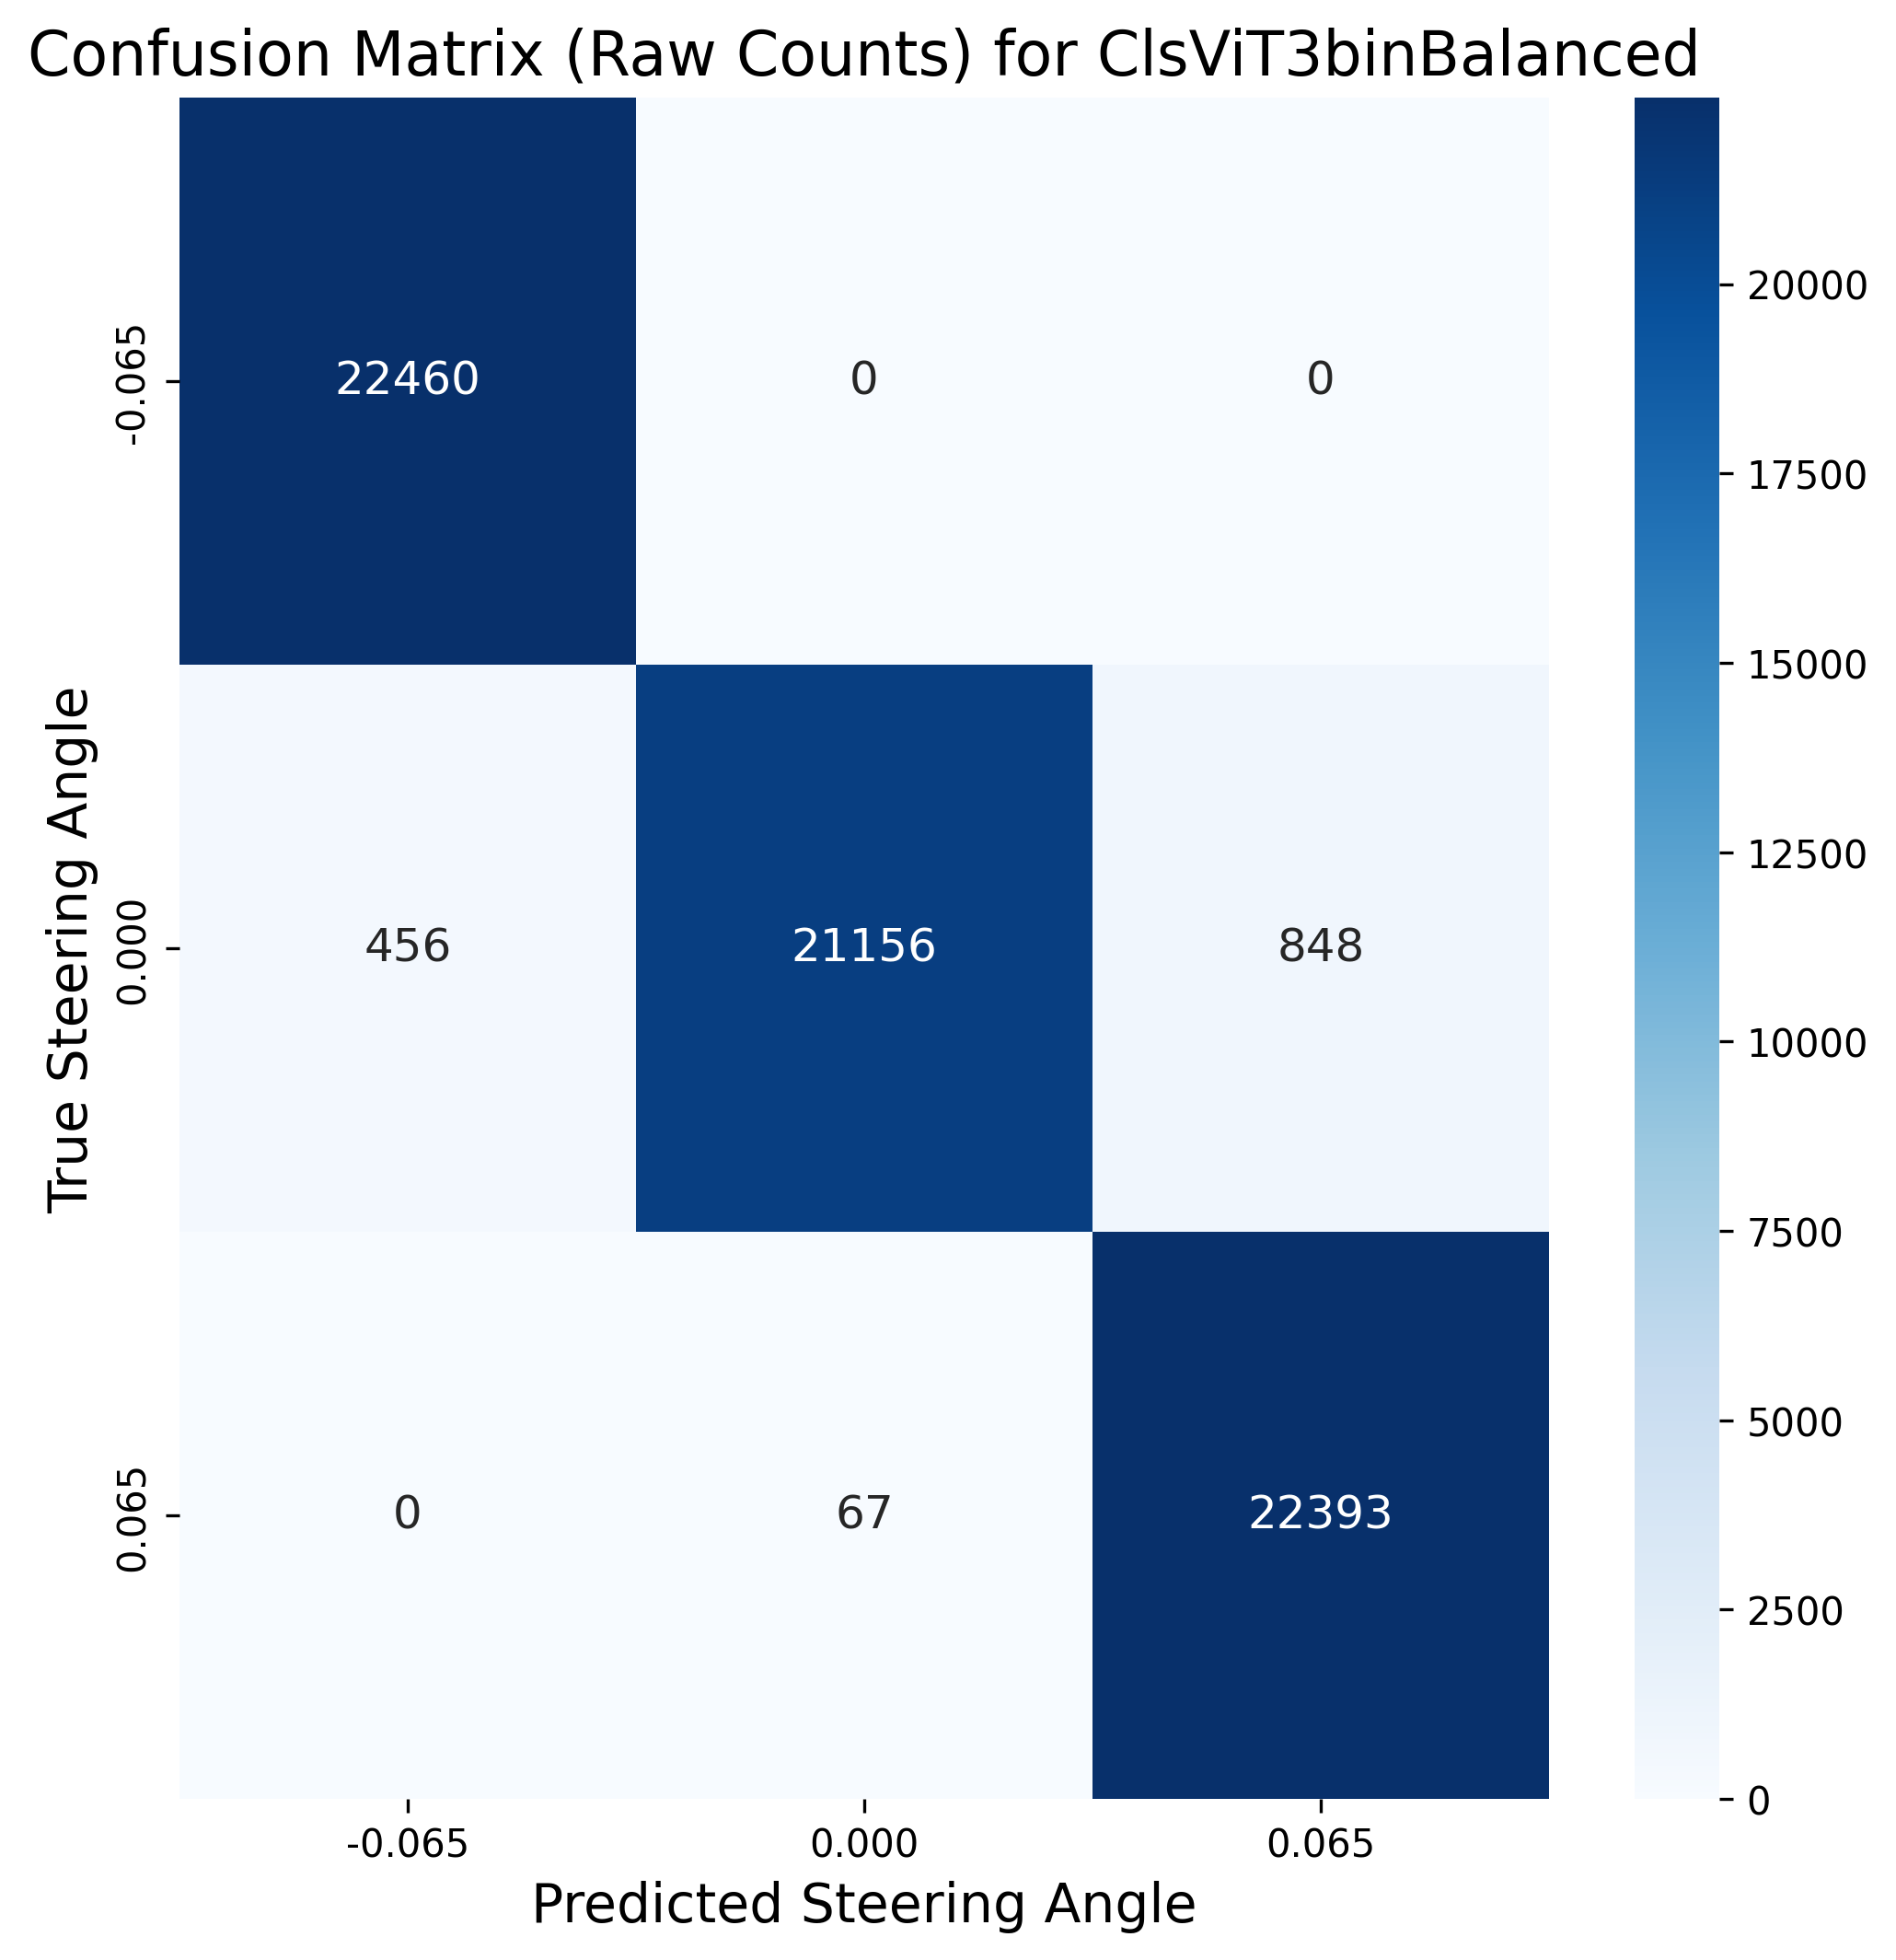
\includegraphics[width=0.65\linewidth]{Figures/Results/cm_raw_ClsViT3binBalanced.png}
\caption{ClsViT3binBalanced model raw counts confusion matrix}
\label{fig:cm_raw_ClsViT3binBalanced}
\end{figure}

\begin{figure}[H]
    \centering
    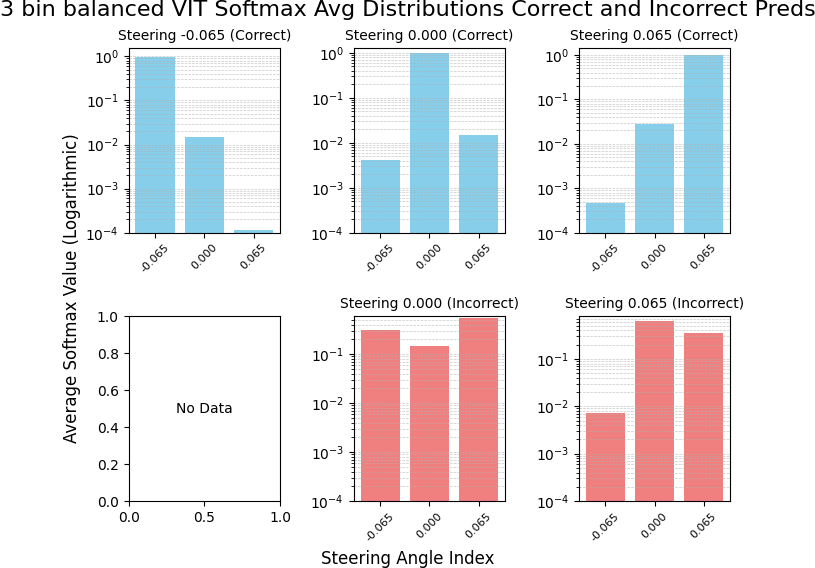
\includegraphics[width=1\linewidth]{Figures/Results/3_bins_vit_softmax_dist_plot_balanced.png}
    \caption{Average Softmax Probabilities for Correctly and Incorrectly Classified Steering Angles in the 3 bin vit balanced training Dataset.}
    \label{fig:3_bins_vit_softmax_dist_balanced}
\end{figure}

%%%%%%%%%%%%%%%%%%%%%%
% ClsViT5binBalanced %
%%%%%%%%%%%%%%%%%%%%%%

\subsubsection{ClsViT5binBalanced}

\begin{table}[htbp]
\centering
\begin{tabular}{@{}lcccc@{}}
\toprule
\textbf{Class} & \textbf{Precision} & \textbf{Recall} & \textbf{F1-Score} & \textbf{Support} \\
\midrule
$-0.065$ & 0.99 & 1.00 & 1.00 & 15,839 \\
$-0.015$ & 0.96 & 0.99 & 0.97 & 15,839 \\
$\phantom{-}0.000$ & 0.99 & 0.95 & 0.97 & 15,839 \\
$\phantom{-}0.015$ & 1.00 & 0.95 & 0.97 & 15,839 \\
$\phantom{-}0.065$ & 0.96 & 1.00 & 0.98 & 15,839 \\
\midrule
\textbf{Macro Avg} & \textbf{0.98} & \textbf{0.98} & \textbf{0.98} & \textbf{79,195} \\
\bottomrule
\end{tabular}
\caption{Classification performance results for the ClsViT5binBalanced model. The model achieved an overall accuracy of 97.77\% with a mean confidence of 0.9779 across 79,195 test images.}
\label{tab:clf_report_ClsViT5binBalanced}
\end{table}

\begin{figure}[H]
\centering
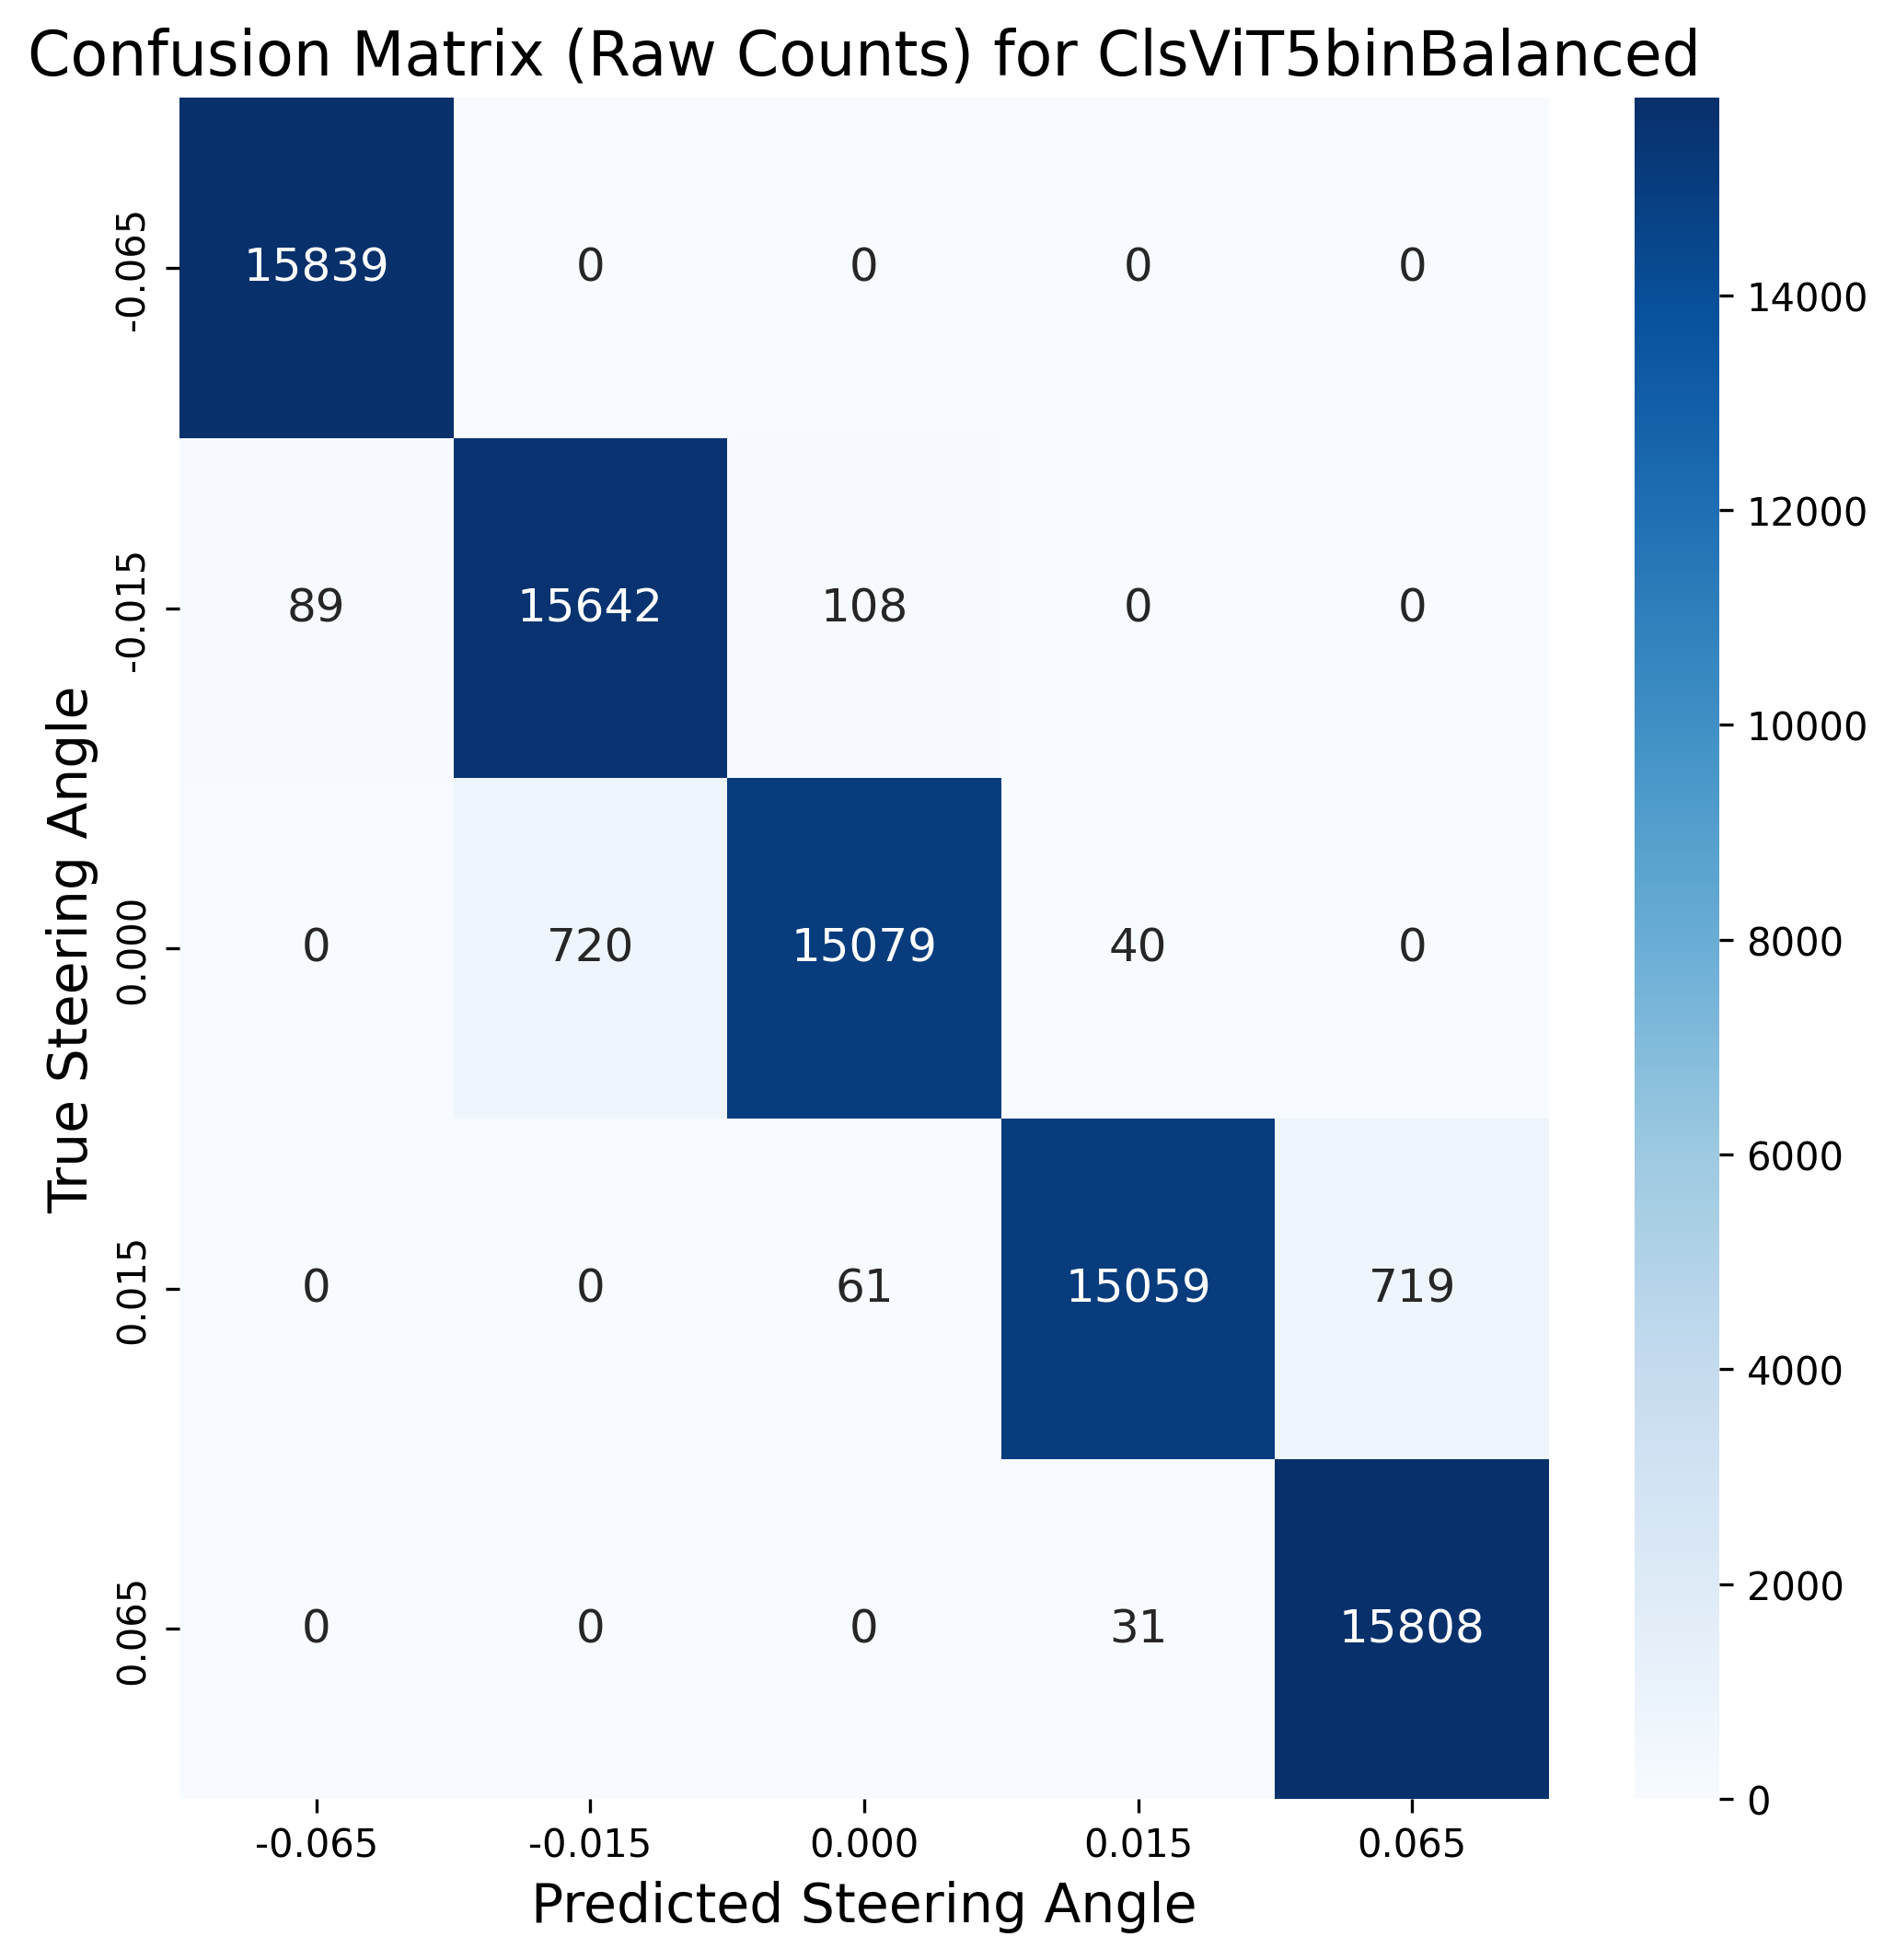
\includegraphics[width=0.65\linewidth]{Figures/Results/cm_raw_ClsViT5binBalanced.png}
\caption{ClsViT5binBalanced model raw counts confusion matrix}
\label{fig:cm_raw_ClsViT5binBalanced}
\end{figure}

\begin{figure}[H]
    \centering
    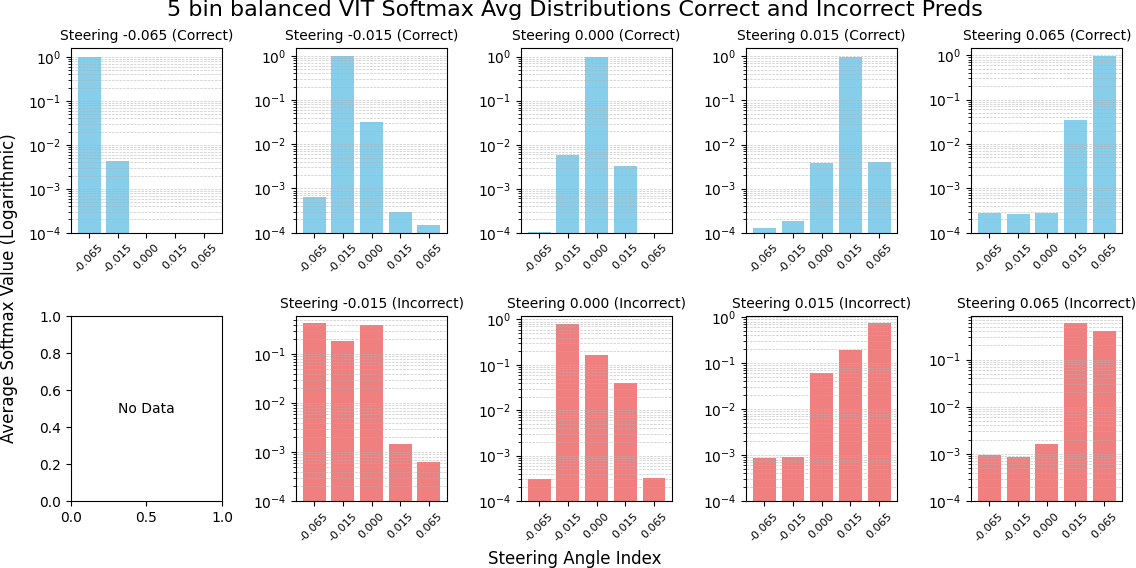
\includegraphics[width=1\linewidth]{Figures/Results/5_bins_vit_softmax_dist_plot_balanced.png}
    \caption{Average Softmax Probabilities for Correctly and Incorrectly Classified Steering Angles in the 5 bin vit balanced training Dataset.}
    \label{fig:5_bins_vit_softmax_dist_balanced}
\end{figure}

\subsection{Additional Analysis of Classifier Outputs}

This section presents the results for the remaining models.

%%%%%%%%%%%%%%%%%%%%%%
% ClsCNN3binBalanced %
%%%%%%%%%%%%%%%%%%%%%%

\subsubsection{ClsCNN3binBalanced}

\begin{table}[htbp]
\centering
\begin{tabular}{@{}lcccc@{}}
\toprule
\textbf{Class} & \textbf{Precision} & \textbf{Recall} & \textbf{F1-Score} & \textbf{Support} \\
\midrule
$-0.065$ & 0.88 & 0.95 & 0.91 & 22,460 \\
$\phantom{-}0.000$ & 0.80 & 0.66 & 0.73 & 22,460 \\
$\phantom{-}0.065$ & 0.81 & 0.89 & 0.85 & 22,460 \\
\midrule
\textbf{Macro Avg} & \textbf{0.83} & \textbf{0.83} & \textbf{0.83} & \textbf{67,380} \\
\bottomrule
\end{tabular}
\caption{Classification performance results for the ClsCNN3binBalanced model. The model achieved an overall accuracy of 83.36\% with a mean confidence of 0.8312 across 67,380 test images.}
\label{tab:clf_report_ClsCNN3binBalanced}
\end{table}

\begin{figure}[H]
\centering
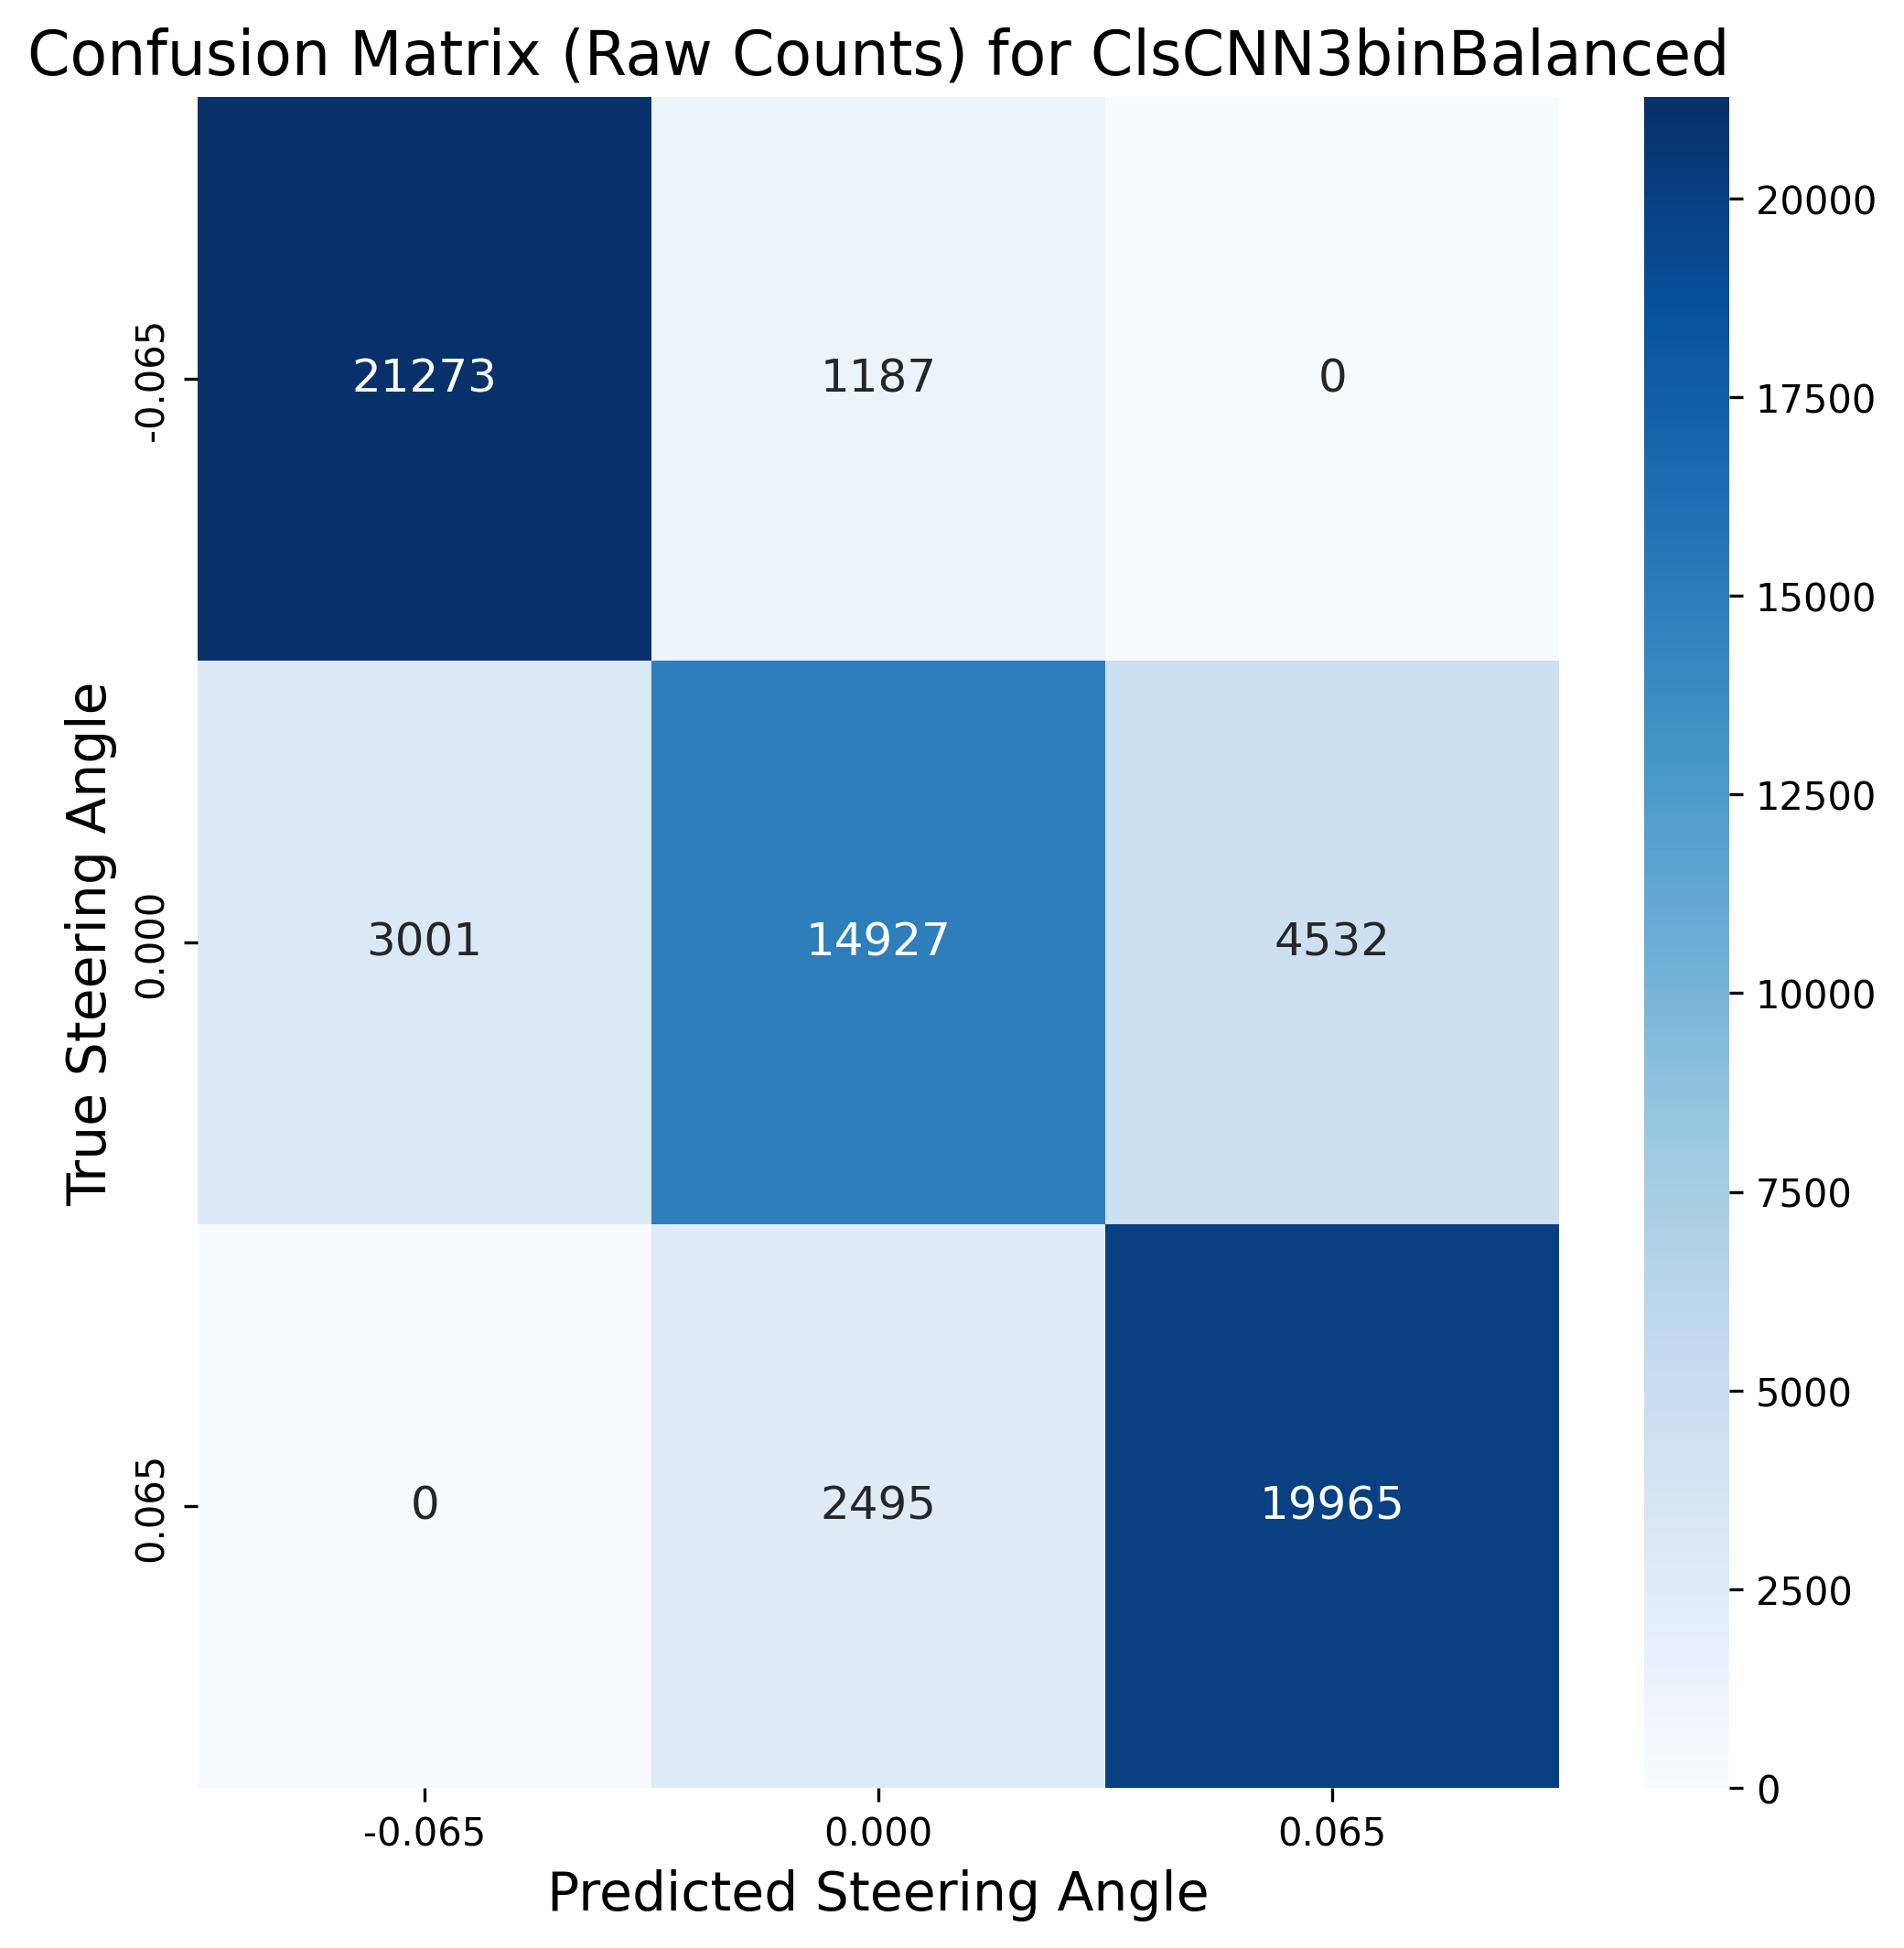
\includegraphics[width=0.65\linewidth]{Figures/Results/cm_raw_ClsCNN3binBalanced.png}
\caption{ClsCNN3binBalanced model raw counts confusion matrix}
\label{fig:cm_raw_ClsCNN3binBalanced}
\end{figure}

\begin{figure}[H]
    \centering
    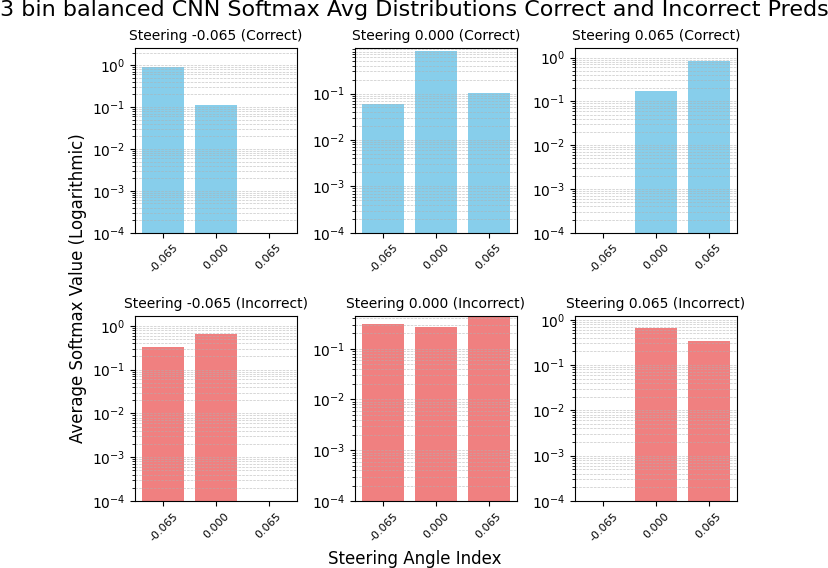
\includegraphics[width=1\linewidth]{Figures/Results/3_bins_cnn_softmax_dist_plot_balanced.png}
    \caption{Average Softmax Probabilities for Correctly and Incorrectly Classified Steering Angles in the 3 bin cnn balanced training Dataset.}
    \label{fig:3_bins_cnn_softmax_dist_balanced}
\end{figure}

%%%%%%%%%%%%%%%%%%%%%%%%
% ClsCNN3binUnbalanced %
%%%%%%%%%%%%%%%%%%%%%%%%

\subsubsection{ClsCNN3binUnbalanced}

\begin{table}[htbp]
\centering
\begin{tabular}{@{}lcccc@{}}
\toprule
\textbf{Class} & \textbf{Precision} & \textbf{Recall} & \textbf{F1-Score} & \textbf{Support} \\
\midrule
$-0.065$ & 0.61 & 0.28 & 0.38 & 1,422 \\
$\phantom{-}0.000$ & 0.89 & 0.97 & 0.93 & 22,460 \\
$\phantom{-}0.065$ & 0.79 & 0.42 & 0.55 & 3,059 \\
\midrule
\textbf{Macro Avg} & \textbf{0.76} & \textbf{0.56} & \textbf{0.62} & \textbf{26,941} \\
\bottomrule
\end{tabular}
\caption{Classification performance results for the ClsCNN3binUnbalanced model. The model achieved an overall accuracy of 87.36\% with a mean confidence of 0.8682 across 26,941 test images.}
\label{tab:clf_report_ClsCNN3binUnbalanced}
\end{table}

\begin{figure}[H]
\centering
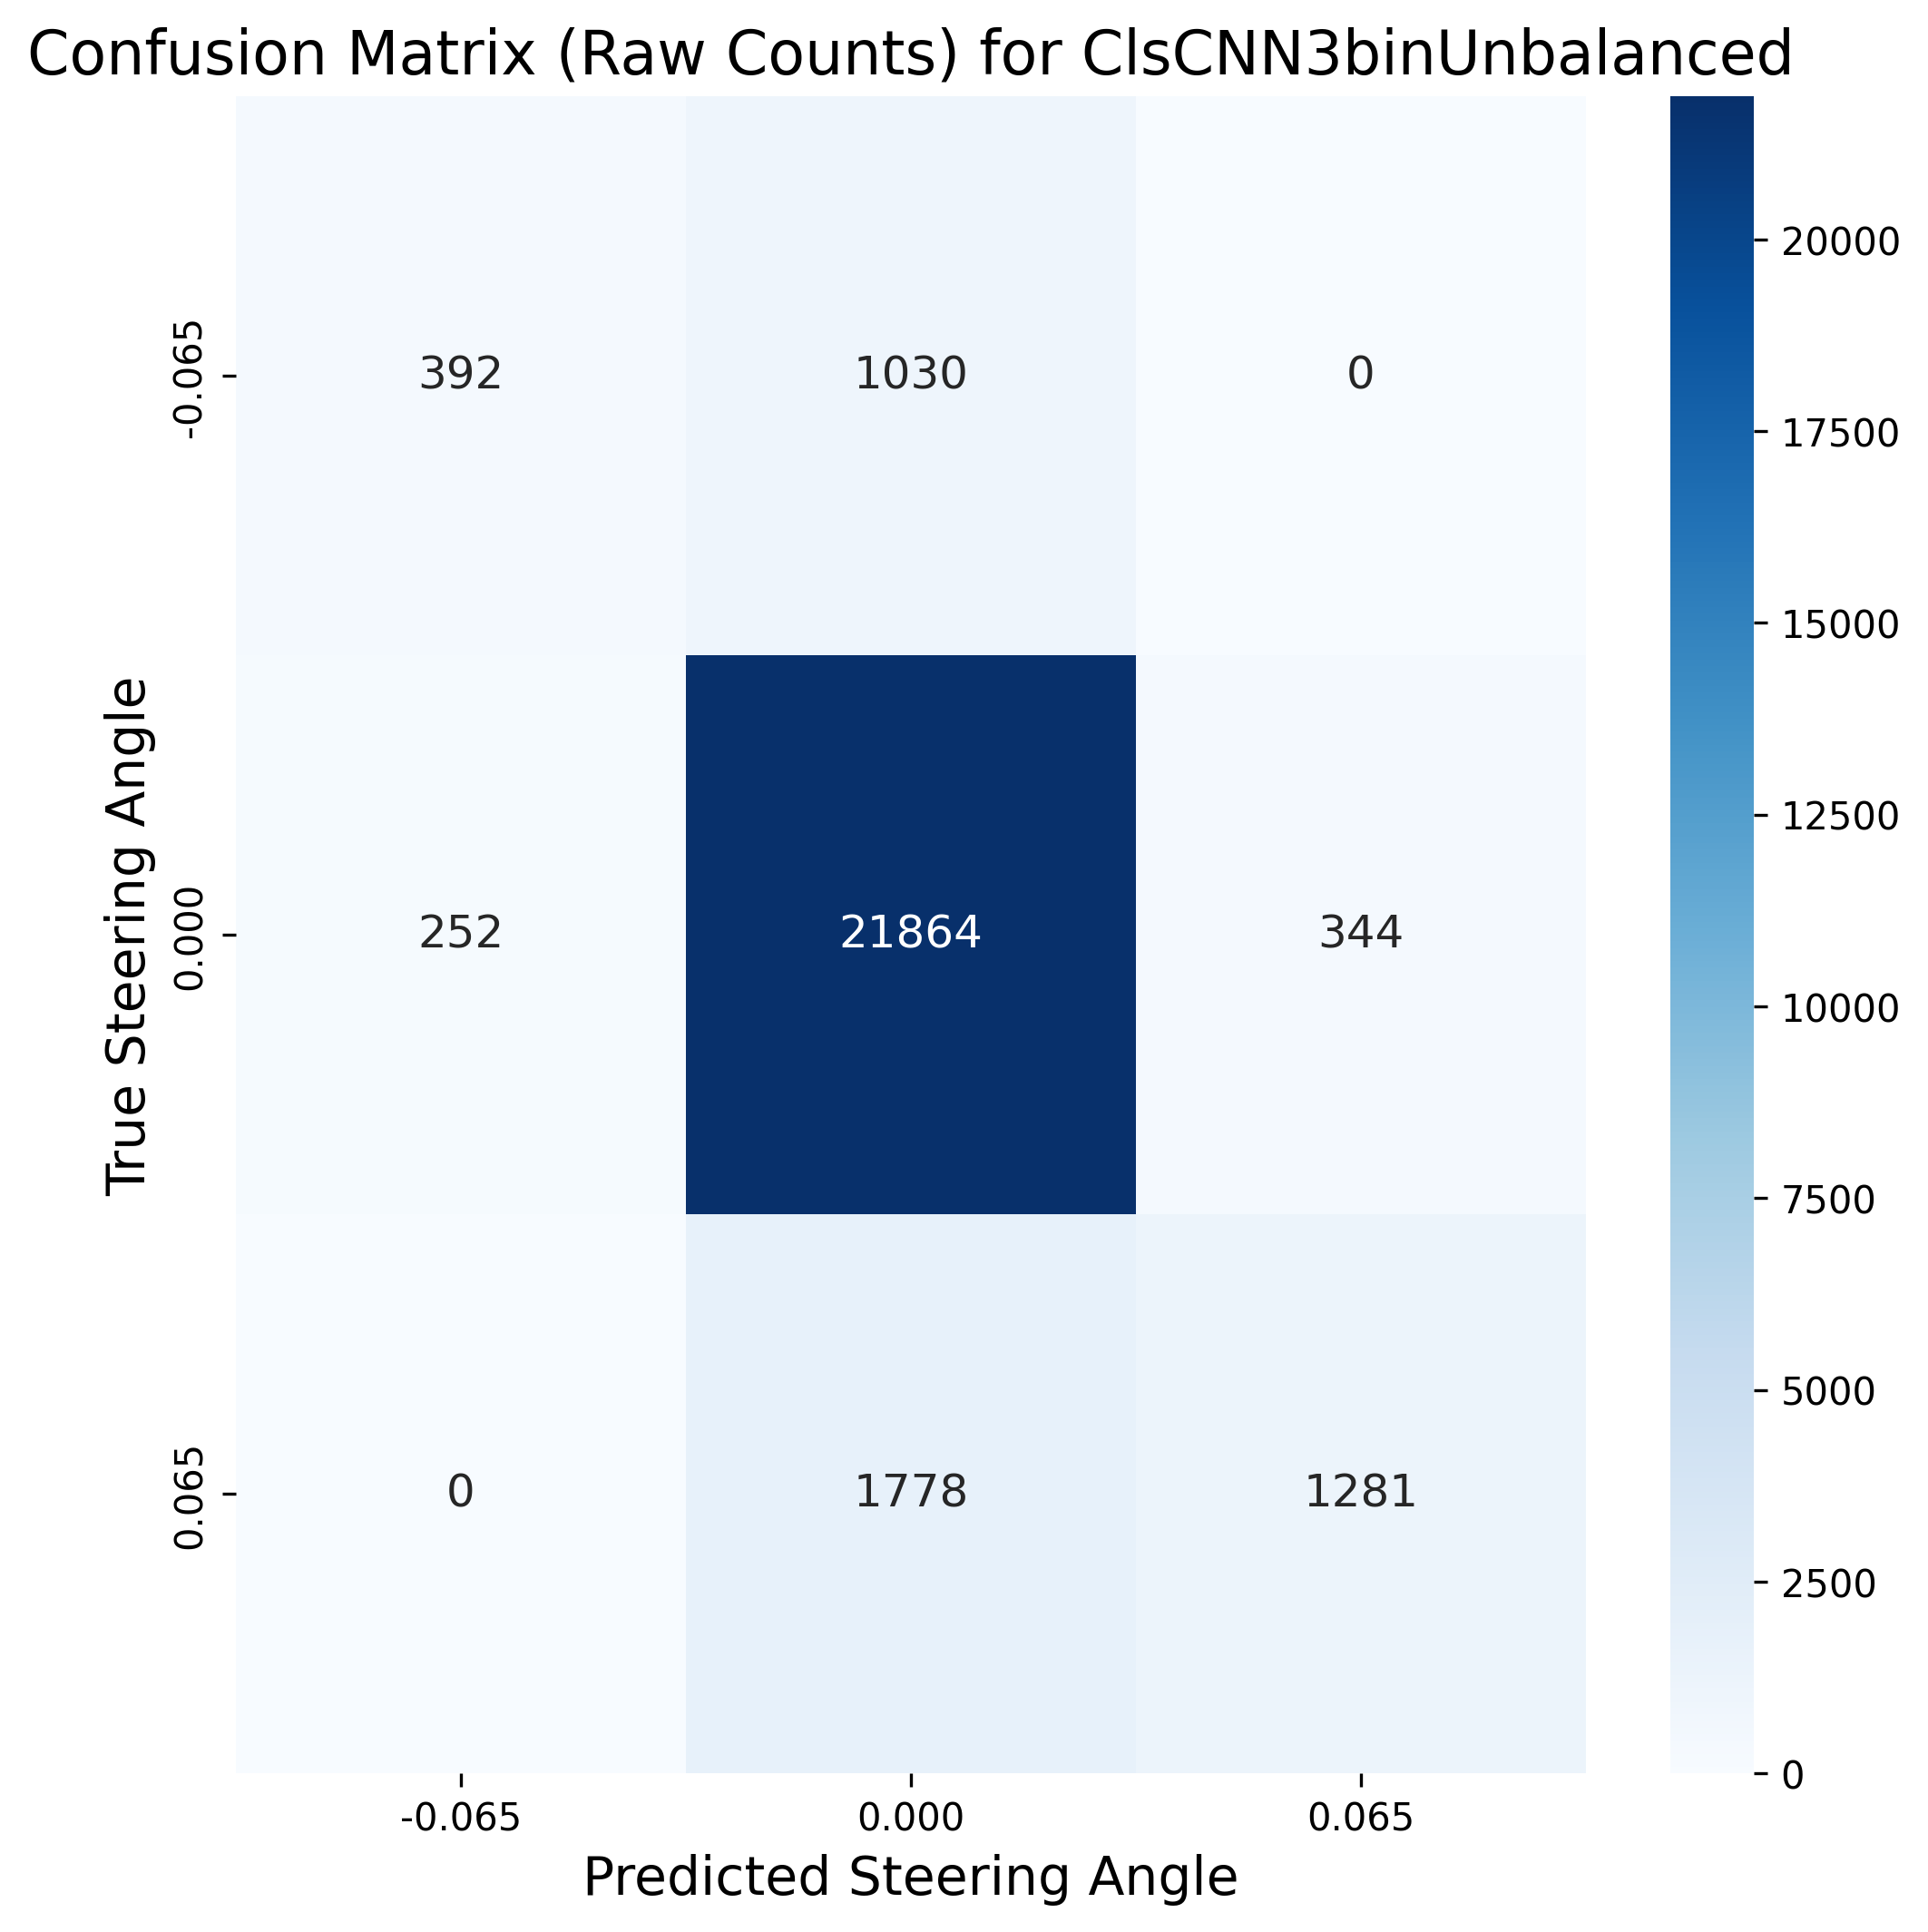
\includegraphics[width=0.65\linewidth]{Figures/Results/cm_raw_ClsCNN3binUnbalanced.png}
\caption{ClsCNN3binUnbalanced model raw counts confusion matrix}
\label{fig:cm_raw_ClsCNN3binUnbalanced}
\end{figure}

\begin{figure}[H]
    \centering
    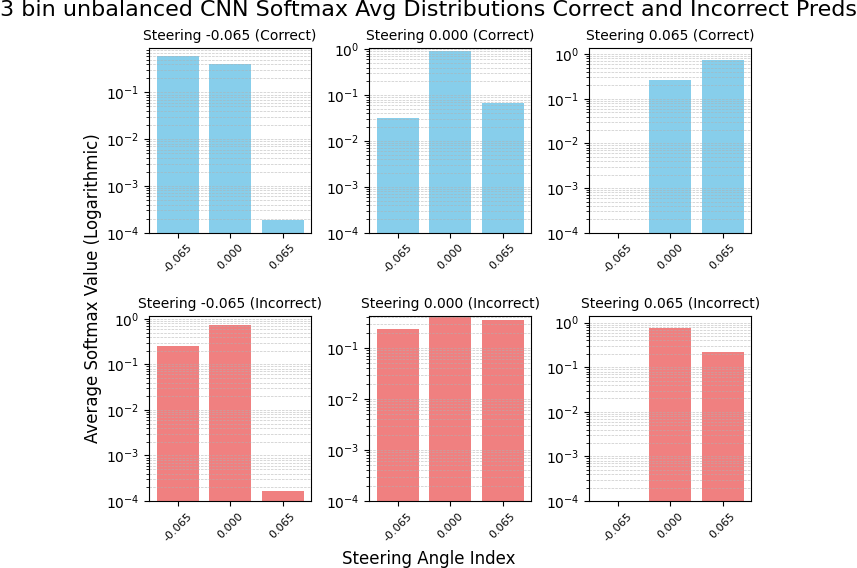
\includegraphics[width=1\linewidth]{Figures/Results/3_bins_cnn_softmax_dist_plot_unbalanced.png}
    \caption{Average Softmax Probabilities for Correctly and Incorrectly Classified Steering Angles in the 3 bin cnn unbalanced training Dataset.}
    \label{fig:3_bins_cnn_softmax_dist_unbalanced}
\end{figure}

%%%%%%%%%%%%%%%%%%%%%%
% ClsCNN5binBalanced %
%%%%%%%%%%%%%%%%%%%%%%

\subsubsection{ClsCNN5binBalanced}

\begin{table}[htbp]
\centering
\begin{tabular}{@{}lcccc@{}}
\toprule
\textbf{Class} & \textbf{Precision} & \textbf{Recall} & \textbf{F1-Score} & \textbf{Support} \\
\midrule
$-0.065$ & 0.89 & 0.99 & 0.94 & 15,839 \\
$-0.015$ & 0.93 & 0.86 & 0.90 & 15,839 \\
$\phantom{-}0.000$ & 0.96 & 0.94 & 0.95 & 15,839 \\
$\phantom{-}0.015$ & 0.73 & 0.92 & 0.82 & 15,839 \\
$\phantom{-}0.065$ & 0.92 & 0.67 & 0.77 & 15,839 \\
\midrule
\textbf{Macro Avg} & \textbf{0.89} & \textbf{0.88} & \textbf{0.88} & \textbf{79,195} \\
\bottomrule
\end{tabular}
\caption{Classification performance results for the ClsCNN5binBalanced model. The model achieved an overall accuracy of 87.70\% with a mean confidence of 0.8762 across 79,195 test images.}
\label{tab:clf_report_ClsCNN5binBalanced}
\end{table}

\begin{figure}[H]
\centering
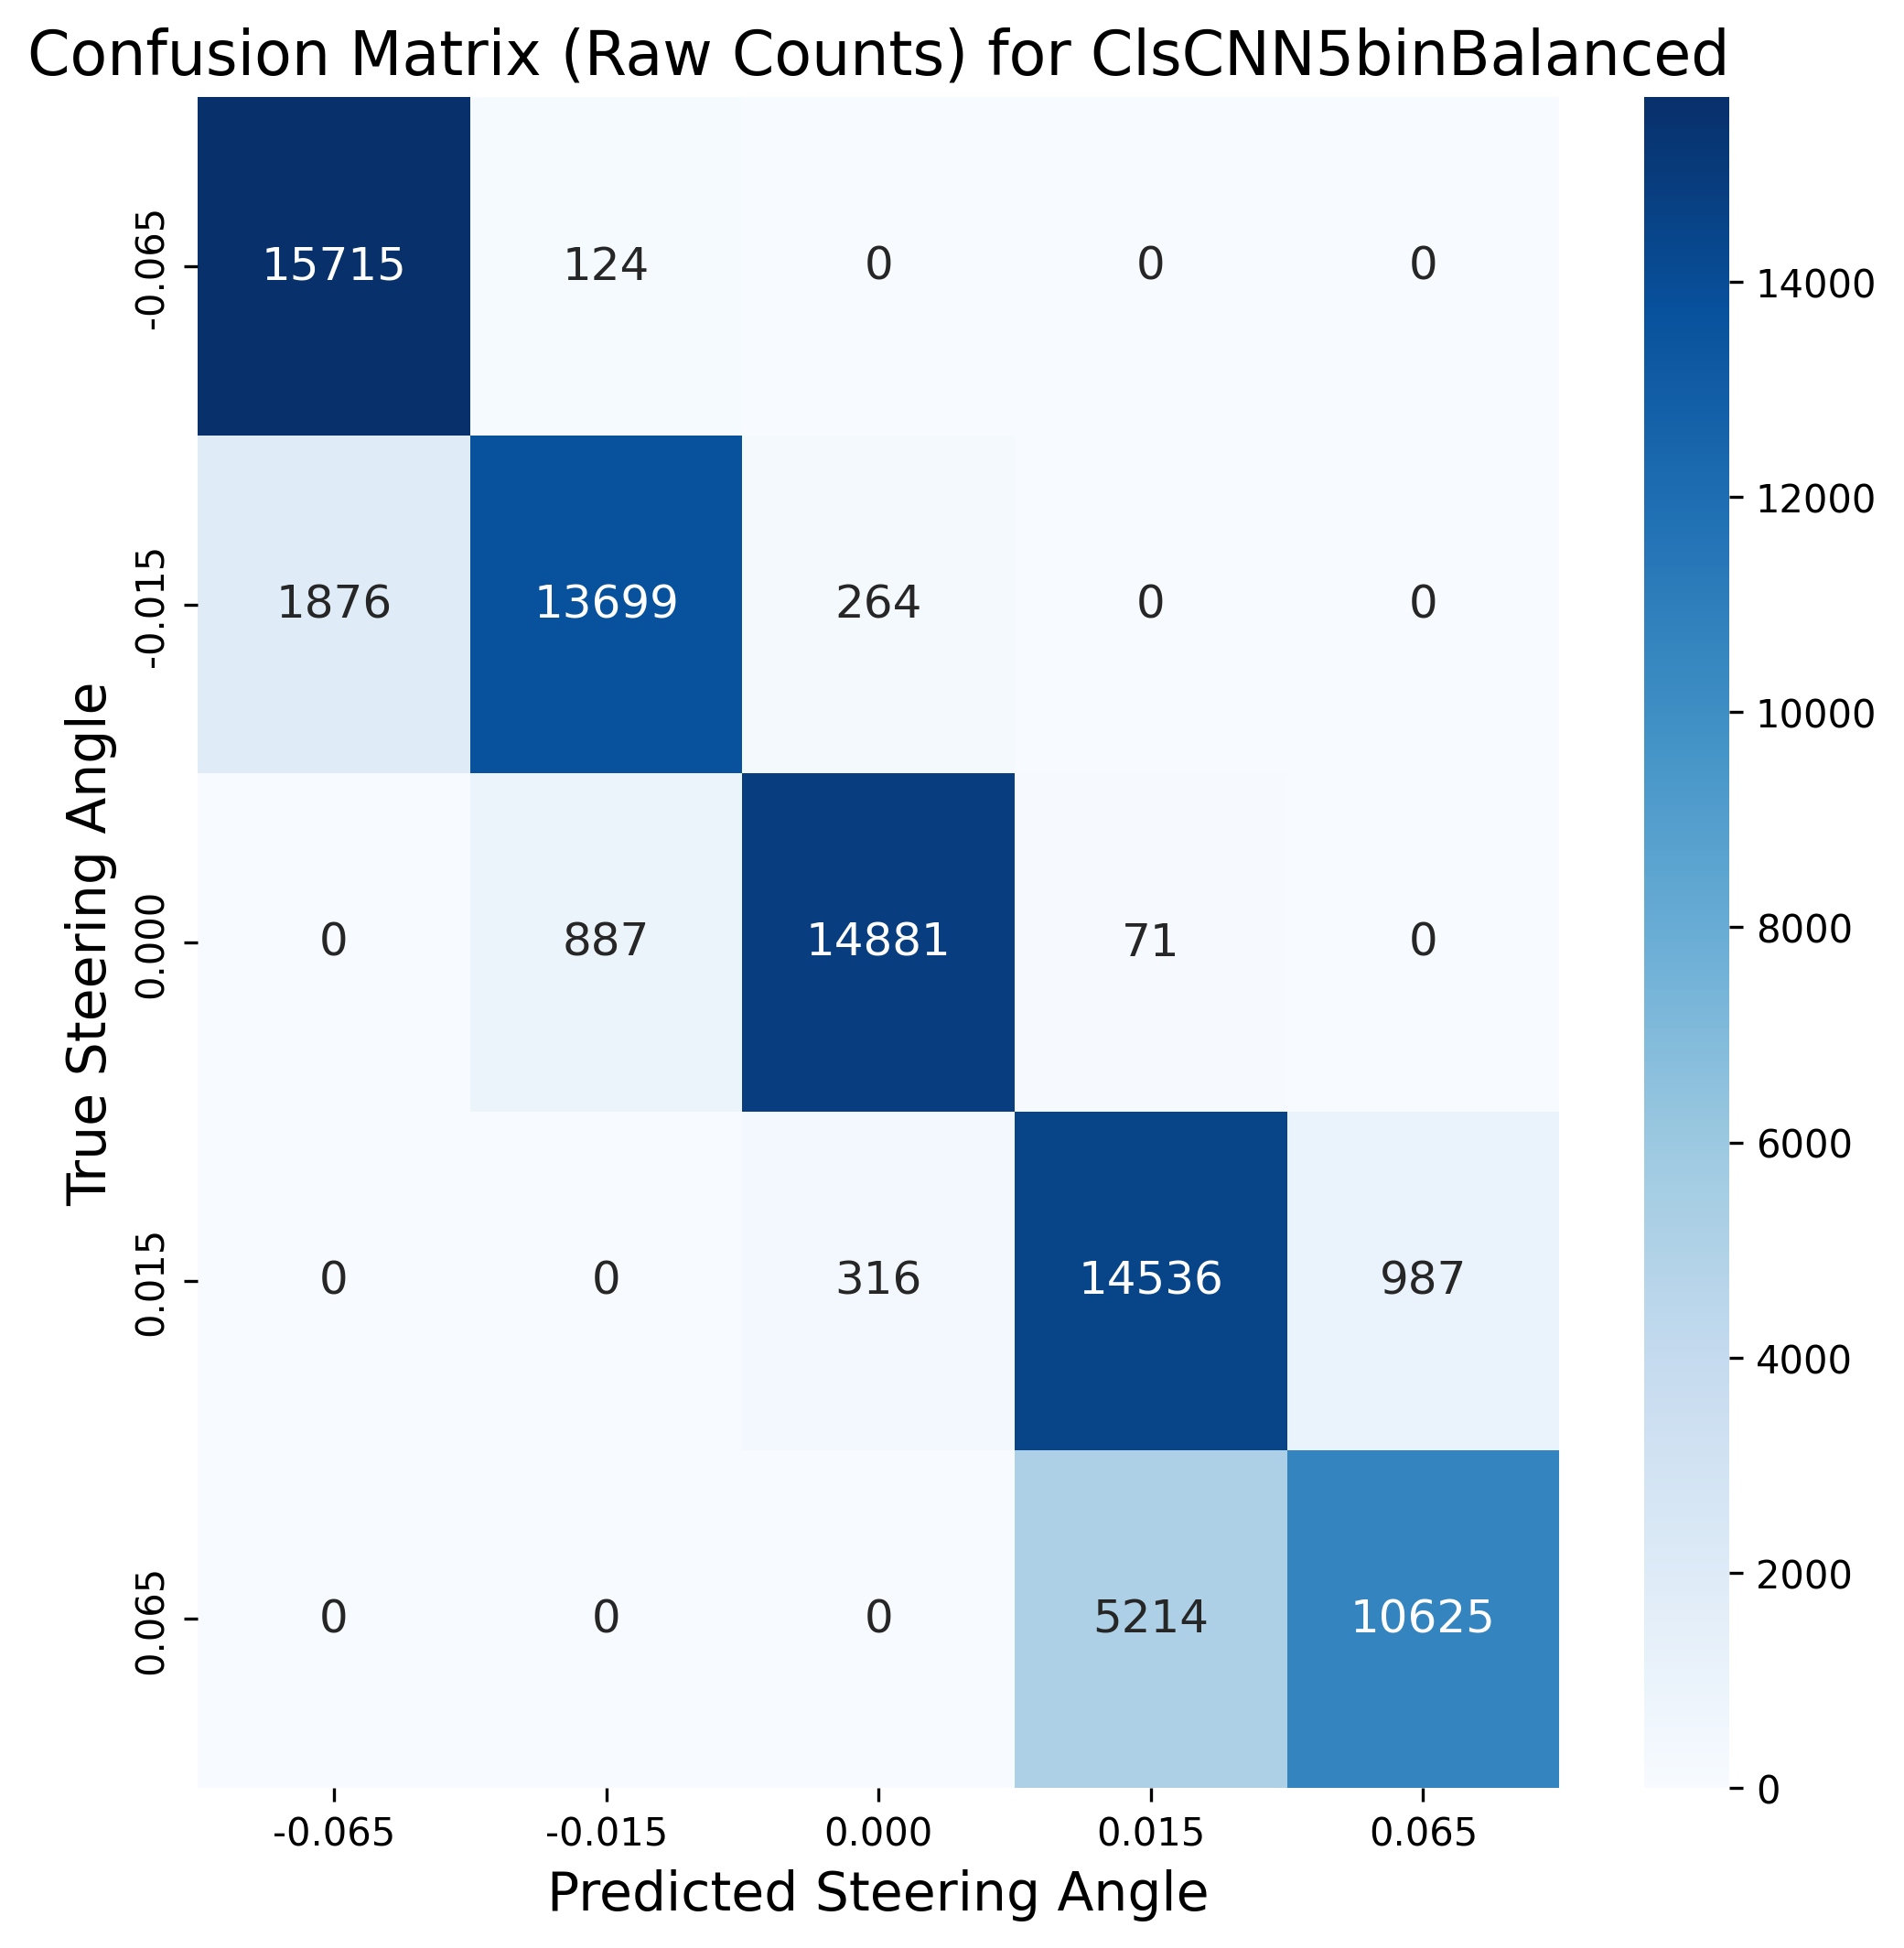
\includegraphics[width=0.65\linewidth]{Figures/Results/cm_raw_ClsCNN5binBalanced.png}
\caption{ClsCNN5binBalanced model raw counts confusion matrix}
\label{fig:cm_raw_ClsCNN5binBalanced}
\end{figure}

\begin{figure}[H]
    \centering
    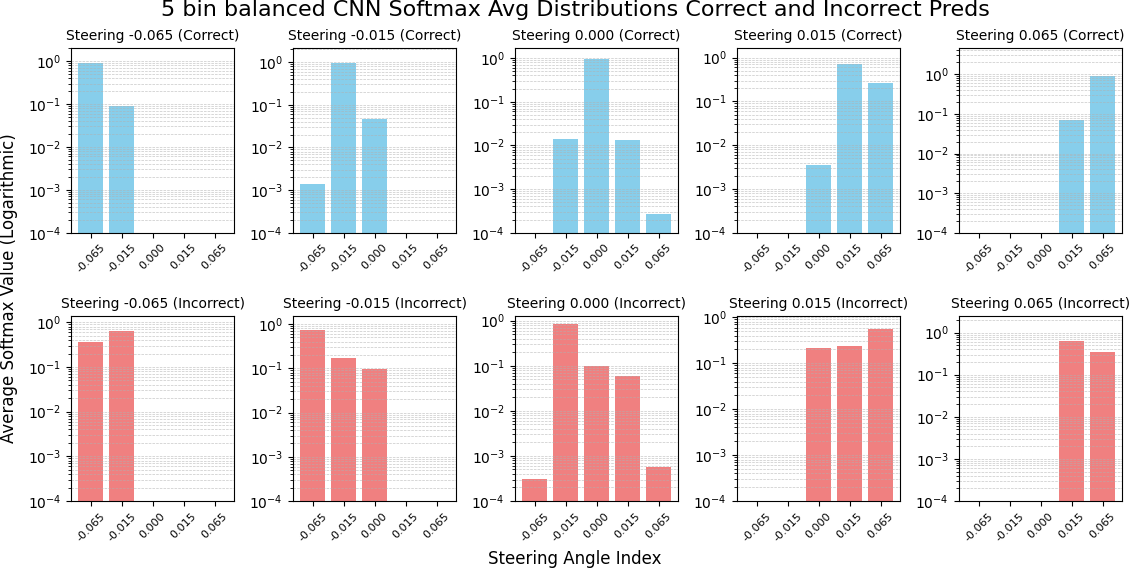
\includegraphics[width=1\linewidth]{Figures/Results/5_bins_cnn_softmax_dist_plot_balanced.png}
    \caption{Average Softmax Probabilities for Correctly and Incorrectly Classified Steering Angles in the 5 bin cnn balanced training Dataset.}
    \label{fig:5_bins_cnn_softmax_dist_balanced}
\end{figure}

%%%%%%%%%%%%%%%%%%%%%%%
% ClsCNN15binBalanced %
%%%%%%%%%%%%%%%%%%%%%%%

\subsubsection{ClsCNN15binBalanced}

\begin{table}[htbp]
\centering
\begin{tabular}{@{}lcccc@{}}
\toprule
\textbf{Class} & \textbf{Precision} & \textbf{Recall} & \textbf{F1-Score} & \textbf{Support} \\
\midrule
$-0.065$ & 0.37 & 0.43 & 0.40 & 10,199 \\
$-0.055$ & 0.22 & 0.27 & 0.24 & 10,199 \\
$-0.045$ & 0.34 & 0.39 & 0.36 & 10,199 \\
$-0.035$ & 0.00 & 0.00 & 0.00 & 10,199 \\
$-0.025$ & 0.40 & 0.60 & 0.48 & 10,199 \\
$-0.015$ & 0.46 & 0.36 & 0.40 & 10,199 \\
$-0.005$ & 0.77 & 0.95 & 0.85 & 10,199 \\
$\phantom{-}0.000$ & 0.85 & 0.94 & 0.89 & 10,199 \\
$\phantom{-}0.005$ & 0.54 & 0.81 & 0.65 & 10,199 \\
$\phantom{-}0.015$ & 0.51 & 0.12 & 0.20 & 10,199 \\
$\phantom{-}0.025$ & 0.46 & 0.40 & 0.43 & 10,199 \\
$\phantom{-}0.035$ & 0.44 & 0.54 & 0.48 & 10,199 \\
$\phantom{-}0.045$ & 0.48 & 0.31 & 0.38 & 10,199 \\
$\phantom{-}0.055$ & 0.38 & 0.77 & 0.51 & 10,199 \\
$\phantom{-}0.065$ & 0.85 & 0.31 & 0.45 & 10,199 \\
\midrule
\textbf{Macro Avg} & \textbf{0.47} & \textbf{0.48} & \textbf{0.45} & \textbf{152,985} \\
\bottomrule
\end{tabular}
\caption{Classification performance results for the ClsCNN15binBalanced model. The model achieved an overall accuracy of 48.01\% with a mean confidence of 0.4809 across 152,985 test images.}
\label{tab:clf_report_ClsCNN15binBalanced}
\end{table}

\begin{figure}[H]
\centering
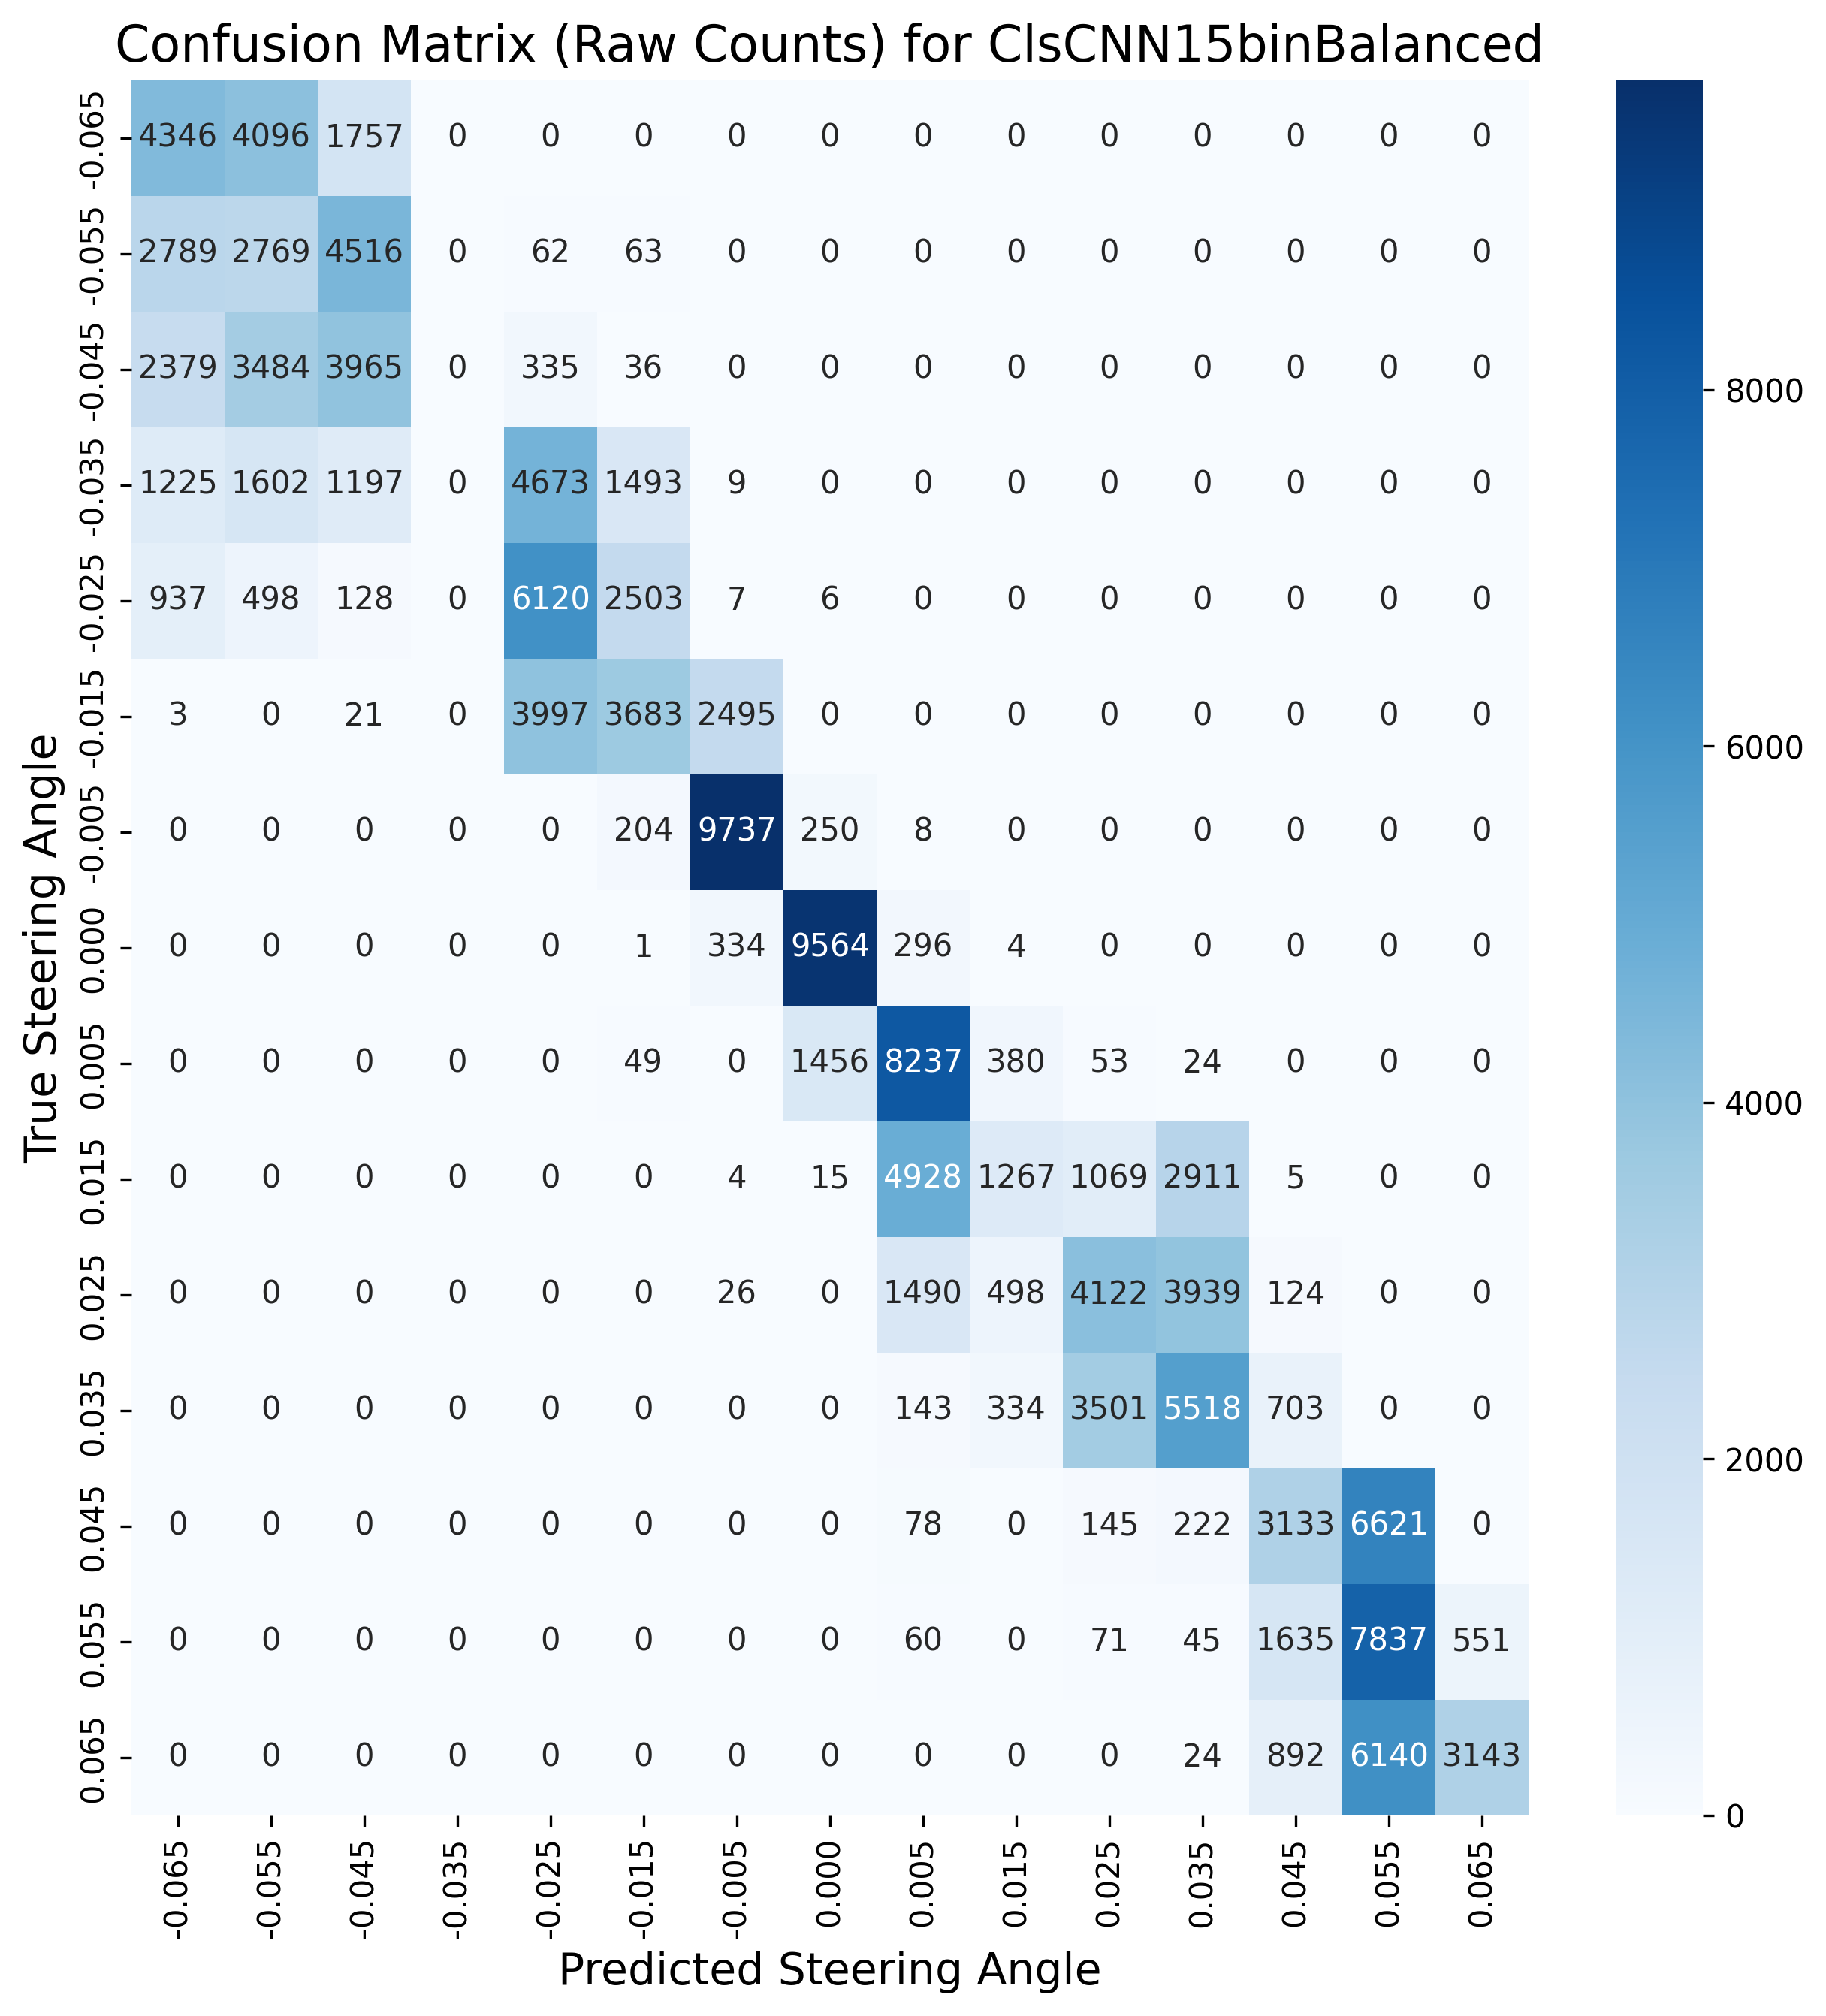
\includegraphics[width=1\linewidth]{Figures/Results/cm_raw_ClsCNN15binBalanced.png}
\caption{ClsCNN15binBalanced model raw counts confusion matrix}
\label{fig:cm_raw_ClsCNN15binBalanced}
\end{figure}

\begin{figure}[H]
    \centering
    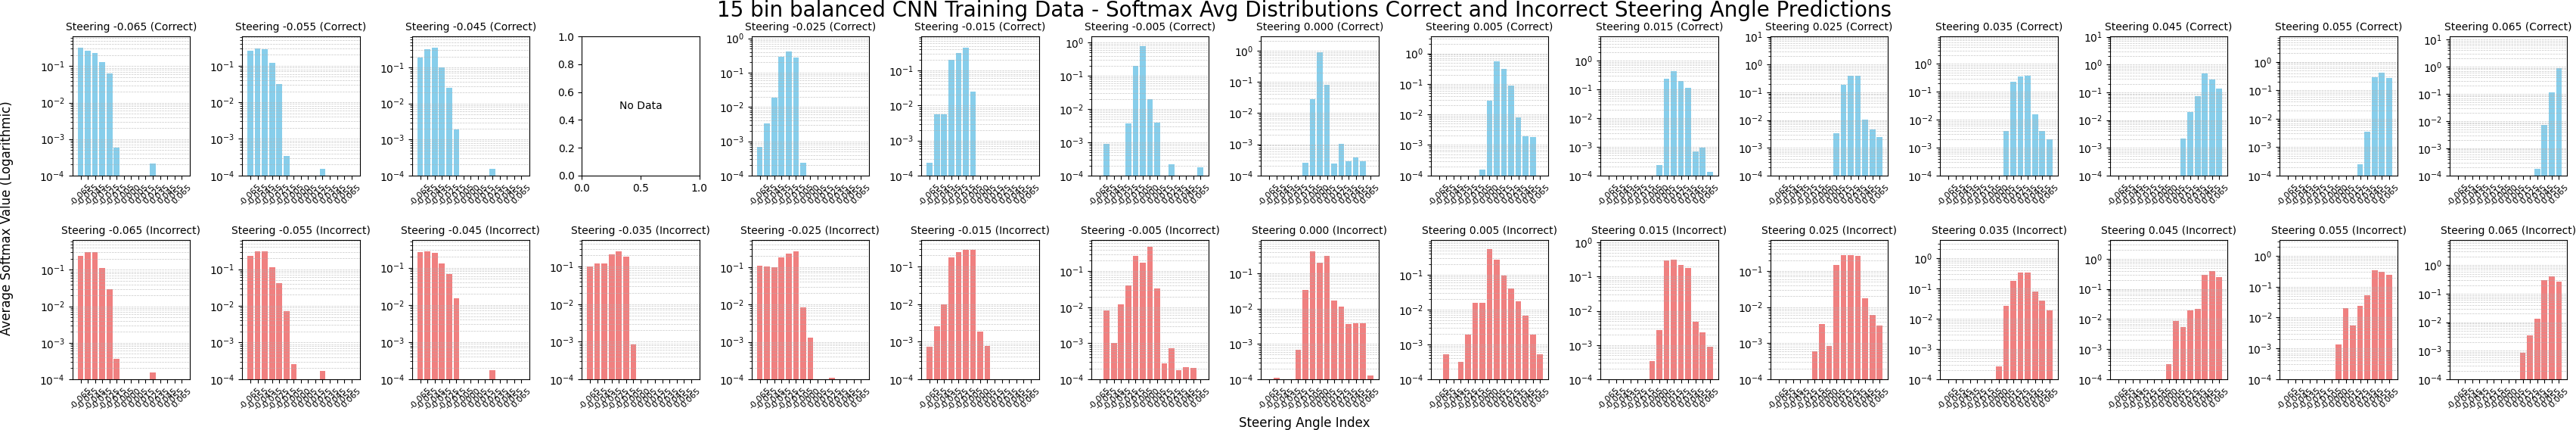
\includegraphics[width=1\linewidth]{Figures/Results/15_bins_cnn_softmax_dist_plot_balanced.png}
    \caption{Average Softmax Probabilities for Correctly and Incorrectly Classified Steering Angles in the 15 bin cnn balanced training Dataset.}
    \label{fig:15_bins_cnn_softmax_dist_balanced}
\end{figure}

%%%%%%%%%%%%%%%%%%%%%%%%%
% ClsCNN15binUnbalanced %
%%%%%%%%%%%%%%%%%%%%%%%%%

\subsubsection{ClsCNN15binUnbalanced}

\begin{table}[htbp]
\centering
\begin{tabular}{@{}lcccc@{}}
\toprule
\textbf{Class} & \textbf{Precision} & \textbf{Recall} & \textbf{F1-Score} & \textbf{Support} \\
\midrule
$-0.065$ & 0.00 & 0.00 & 0.00 & 128 \\
$-0.055$ & 0.00 & 0.00 & 0.00 & 141 \\
$-0.045$ & 0.00 & 0.00 & 0.00 & 223 \\
$-0.035$ & 0.35 & 0.37 & 0.36 & 1,027 \\
$-0.025$ & 0.49 & 0.04 & 0.07 & 2,094 \\
$-0.015$ & 0.60 & 0.74 & 0.66 & 4,986 \\
$-0.005$ & 0.87 & 0.96 & 0.91 & 10,199 \\
$\phantom{-}0.000$ & 0.91 & 0.96 & 0.93 & 4,896 \\
$\phantom{-}0.005$ & 0.00 & 0.00 & 0.00 & 883 \\
$\phantom{-}0.015$ & 0.63 & 0.91 & 0.75 & 2,665 \\
$\phantom{-}0.025$ & 0.47 & 0.32 & 0.38 & 827 \\
$\phantom{-}0.035$ & 0.00 & 0.00 & 0.00 & 240 \\
$\phantom{-}0.045$ & 0.00 & 0.00 & 0.00 & 124 \\
$\phantom{-}0.055$ & 0.00 & 0.00 & 0.00 & 150 \\
$\phantom{-}0.065$ & 0.58 & 0.99 & 0.73 & 408 \\
\midrule
\textbf{Macro Avg} & \textbf{0.33} & \textbf{0.35} & \textbf{0.32} & \textbf{28,991} \\
\bottomrule
\end{tabular}
\caption{Classification performance results for the ClsCNN15binUnbalanced model. The model achieved an overall accuracy of 75.11\% with a mean confidence of 0.7495 across 28,991 test images.}
\label{tab:clf_report_ClsCNN15binUnbalanced}
\end{table}

\begin{figure}[H]
\centering
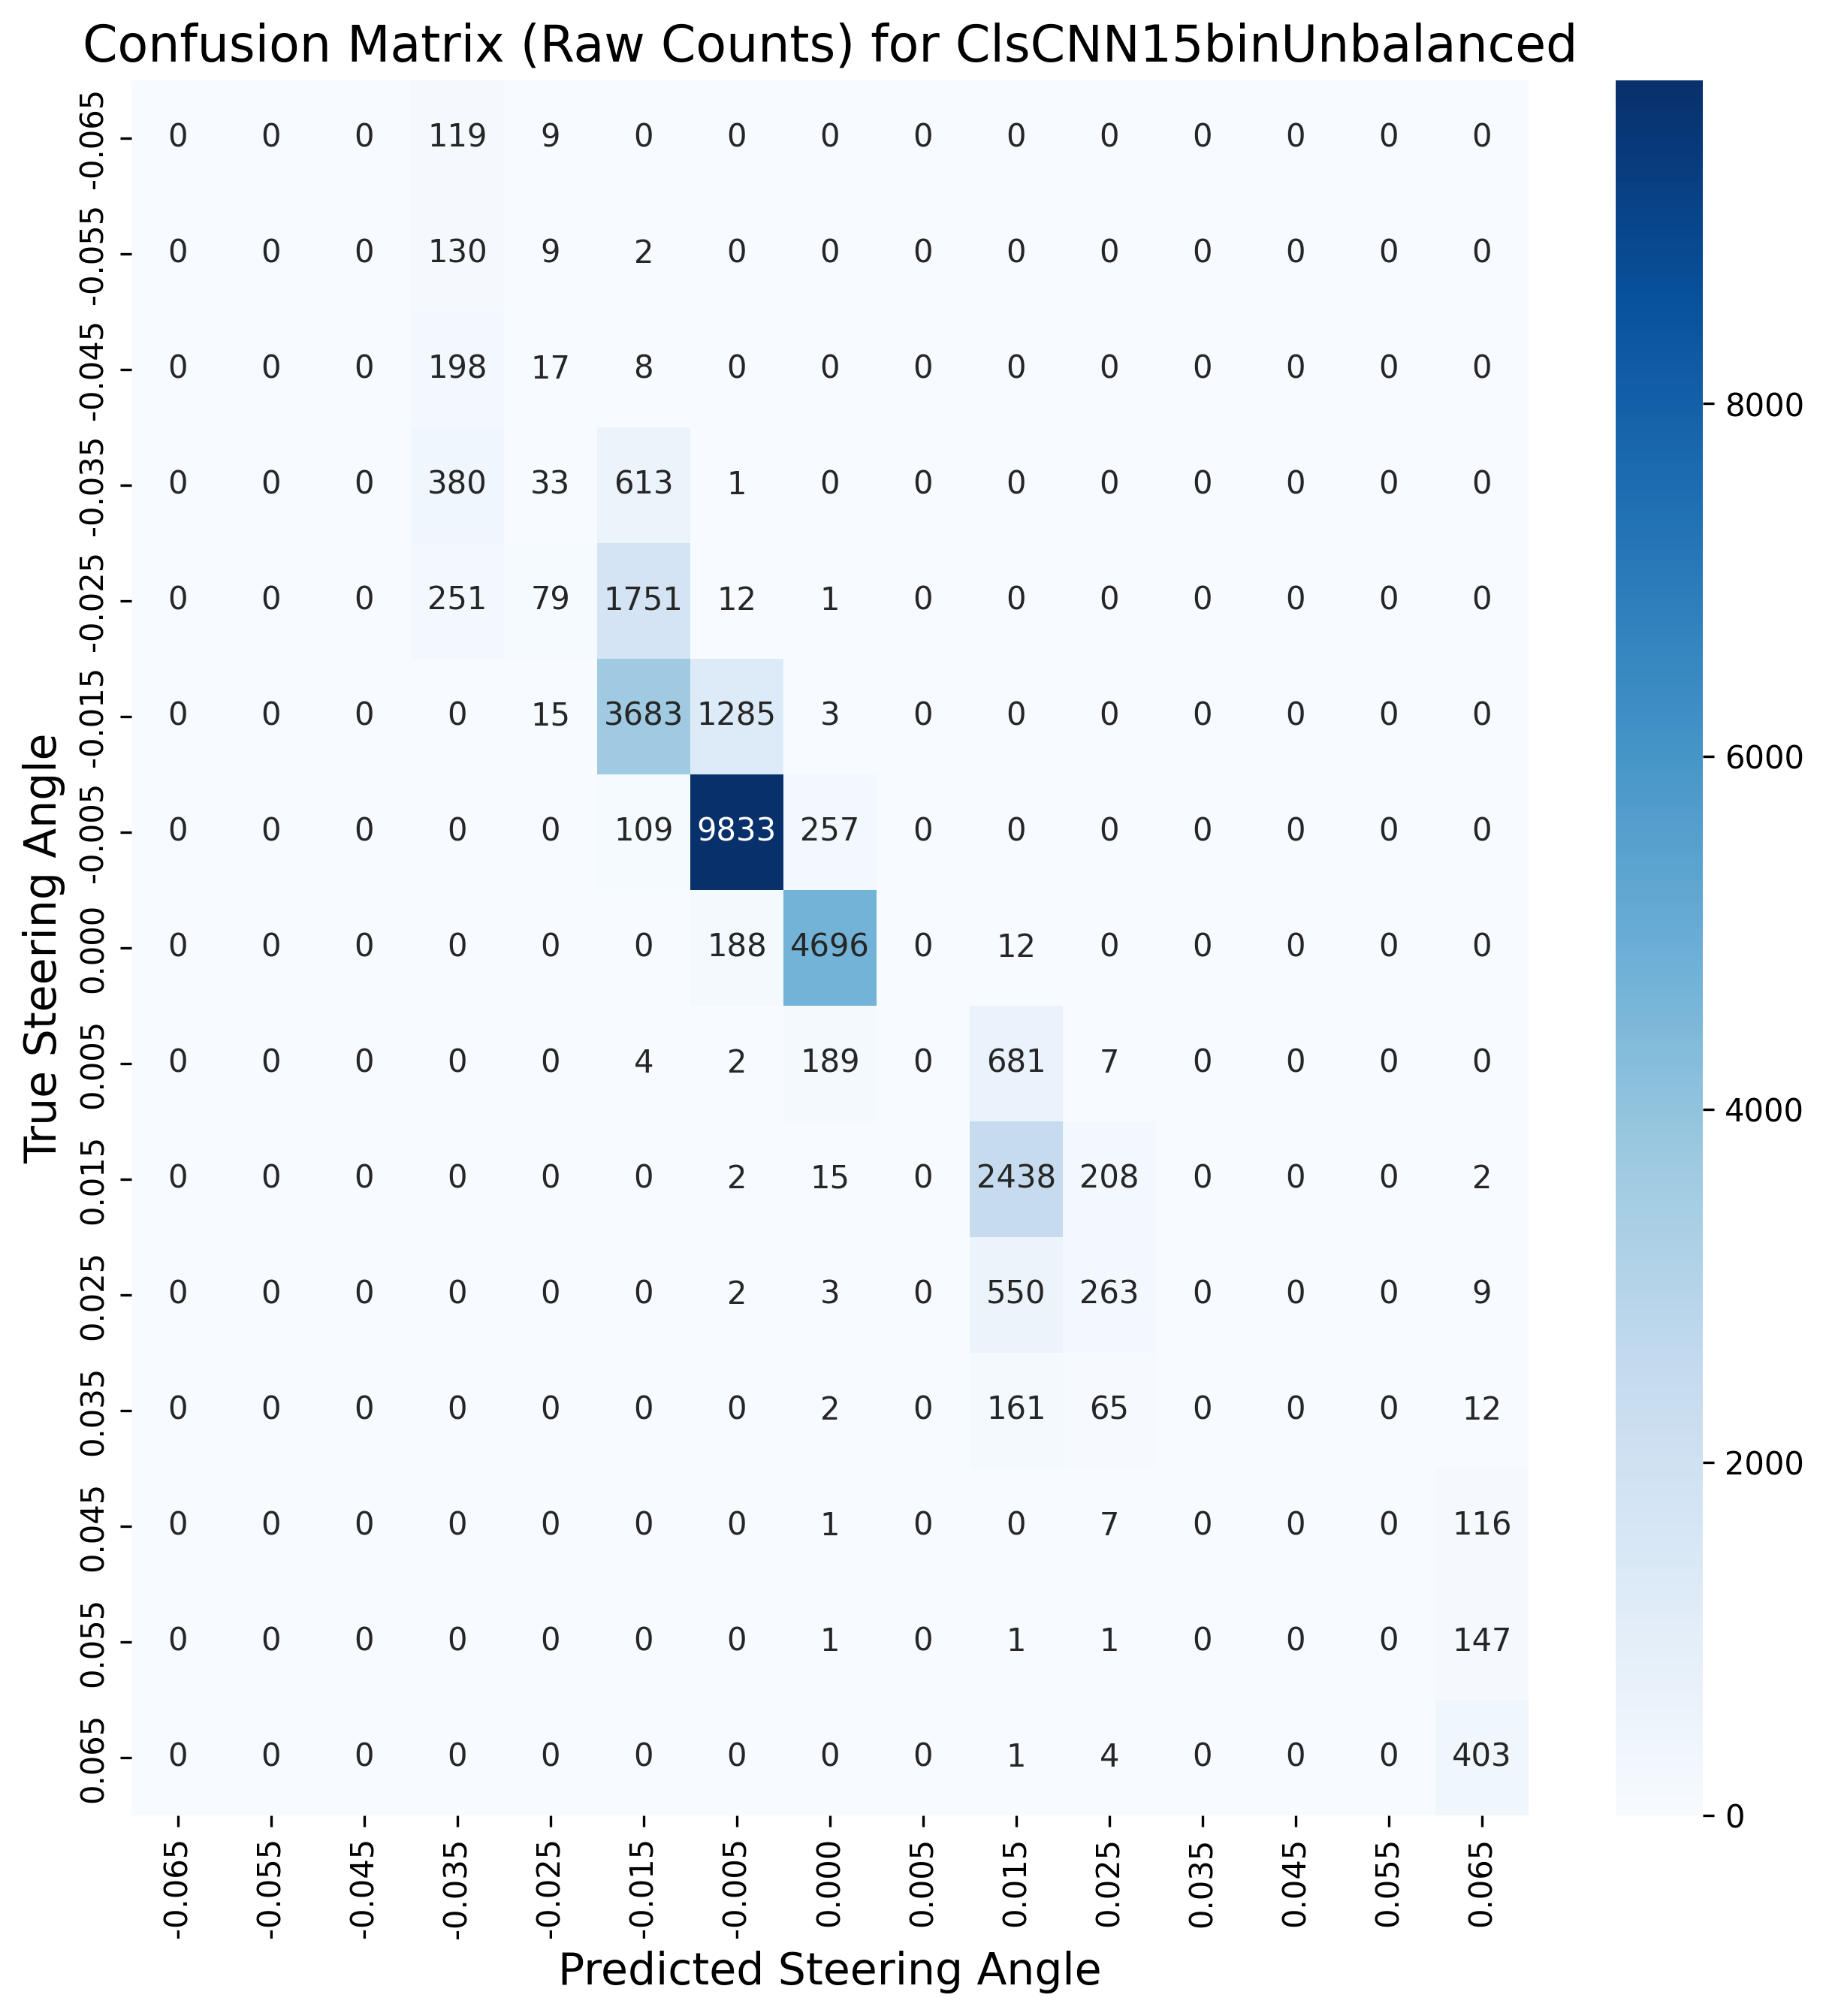
\includegraphics[width=1\linewidth]{Figures/Results/cm_raw_ClsCNN15binUnbalanced.png}
\caption{ClsCNN15binUnbalanced model raw counts confusion matrix}
\label{fig:cm_raw_ClsCNN15binUnbalanced}
\end{figure}

\begin{figure}[H]
    \centering
    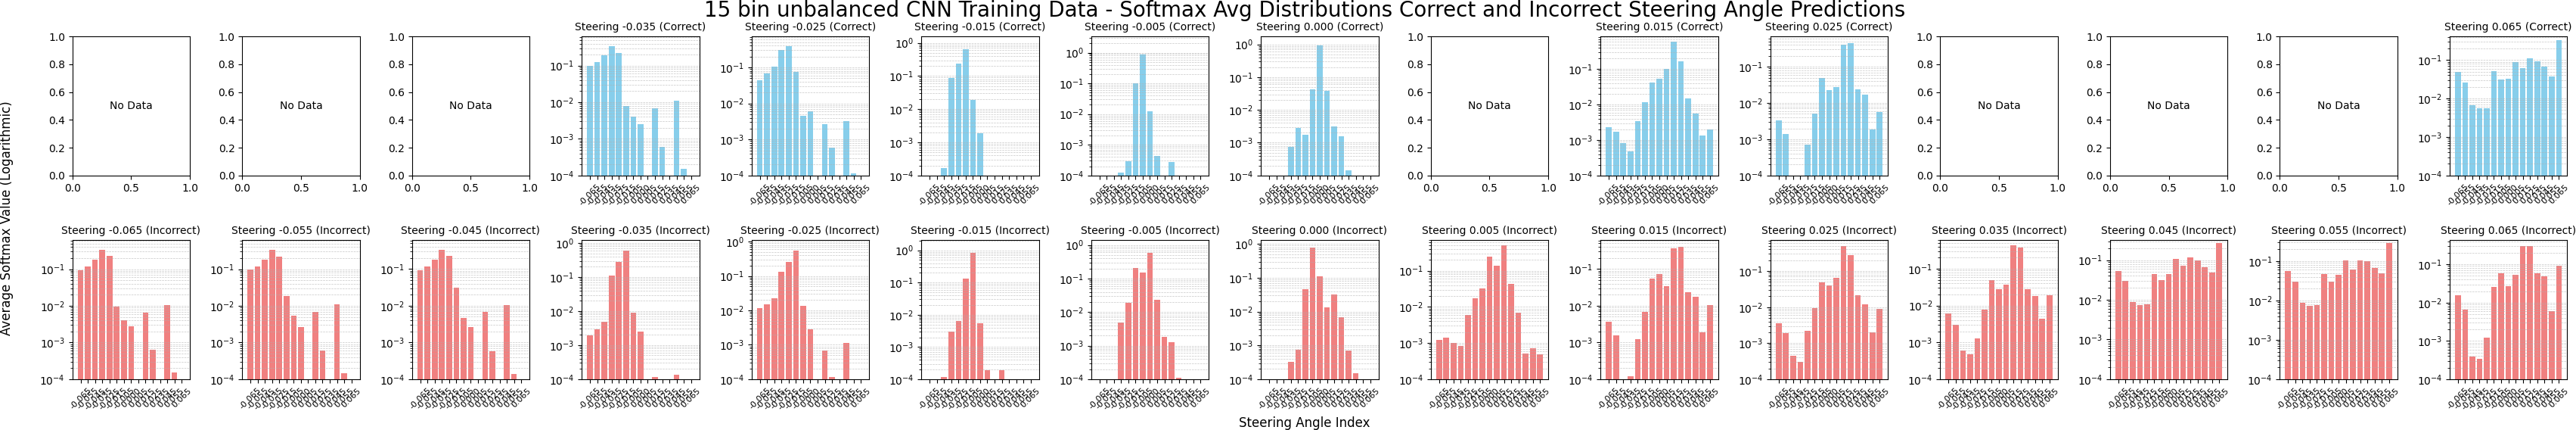
\includegraphics[width=1\linewidth]{Figures/Results/15_bins_cnn_softmax_dist_plot_unbalanced.png}
    \caption{Average Softmax Probabilities for Correctly and Incorrectly Classified Steering Angles in the 15 bin cnn unbalanced training Dataset.}
    \label{fig:15_bins_cnn_softmax_dist_unbalanced}
\end{figure}

%%%%%%%%%%%%%%%%%%%%%%%%
% ClsViT3binUnbalanced %
%%%%%%%%%%%%%%%%%%%%%%%%

\subsubsection{ClsViT3binUnbalanced}

\begin{table}[htbp]
\centering
\begin{tabular}{@{}lcccc@{}}
\toprule
\textbf{Class} & \textbf{Precision} & \textbf{Recall} & \textbf{F1-Score} & \textbf{Support} \\
\midrule
$-0.065$ & 0.82 & 0.66 & 0.73 & 1,422 \\
$\phantom{-}0.000$ & 0.94 & 0.98 & 0.96 & 22,460 \\
$\phantom{-}0.065$ & 0.86 & 0.67 & 0.75 & 3,059 \\
\midrule
\textbf{Macro Avg} & \textbf{0.87} & \textbf{0.77} & \textbf{0.81} & \textbf{26,941} \\
\bottomrule
\end{tabular}
\caption{Classification performance results for the ClsViT3binUnbalanced model. The model achieved an overall accuracy of 92.50\% with a mean confidence of 0.9211 across 26,941 test images.}
\label{tab:clf_report_ClsViT3binUnbalanced}
\end{table}

\begin{figure}[H]
\centering
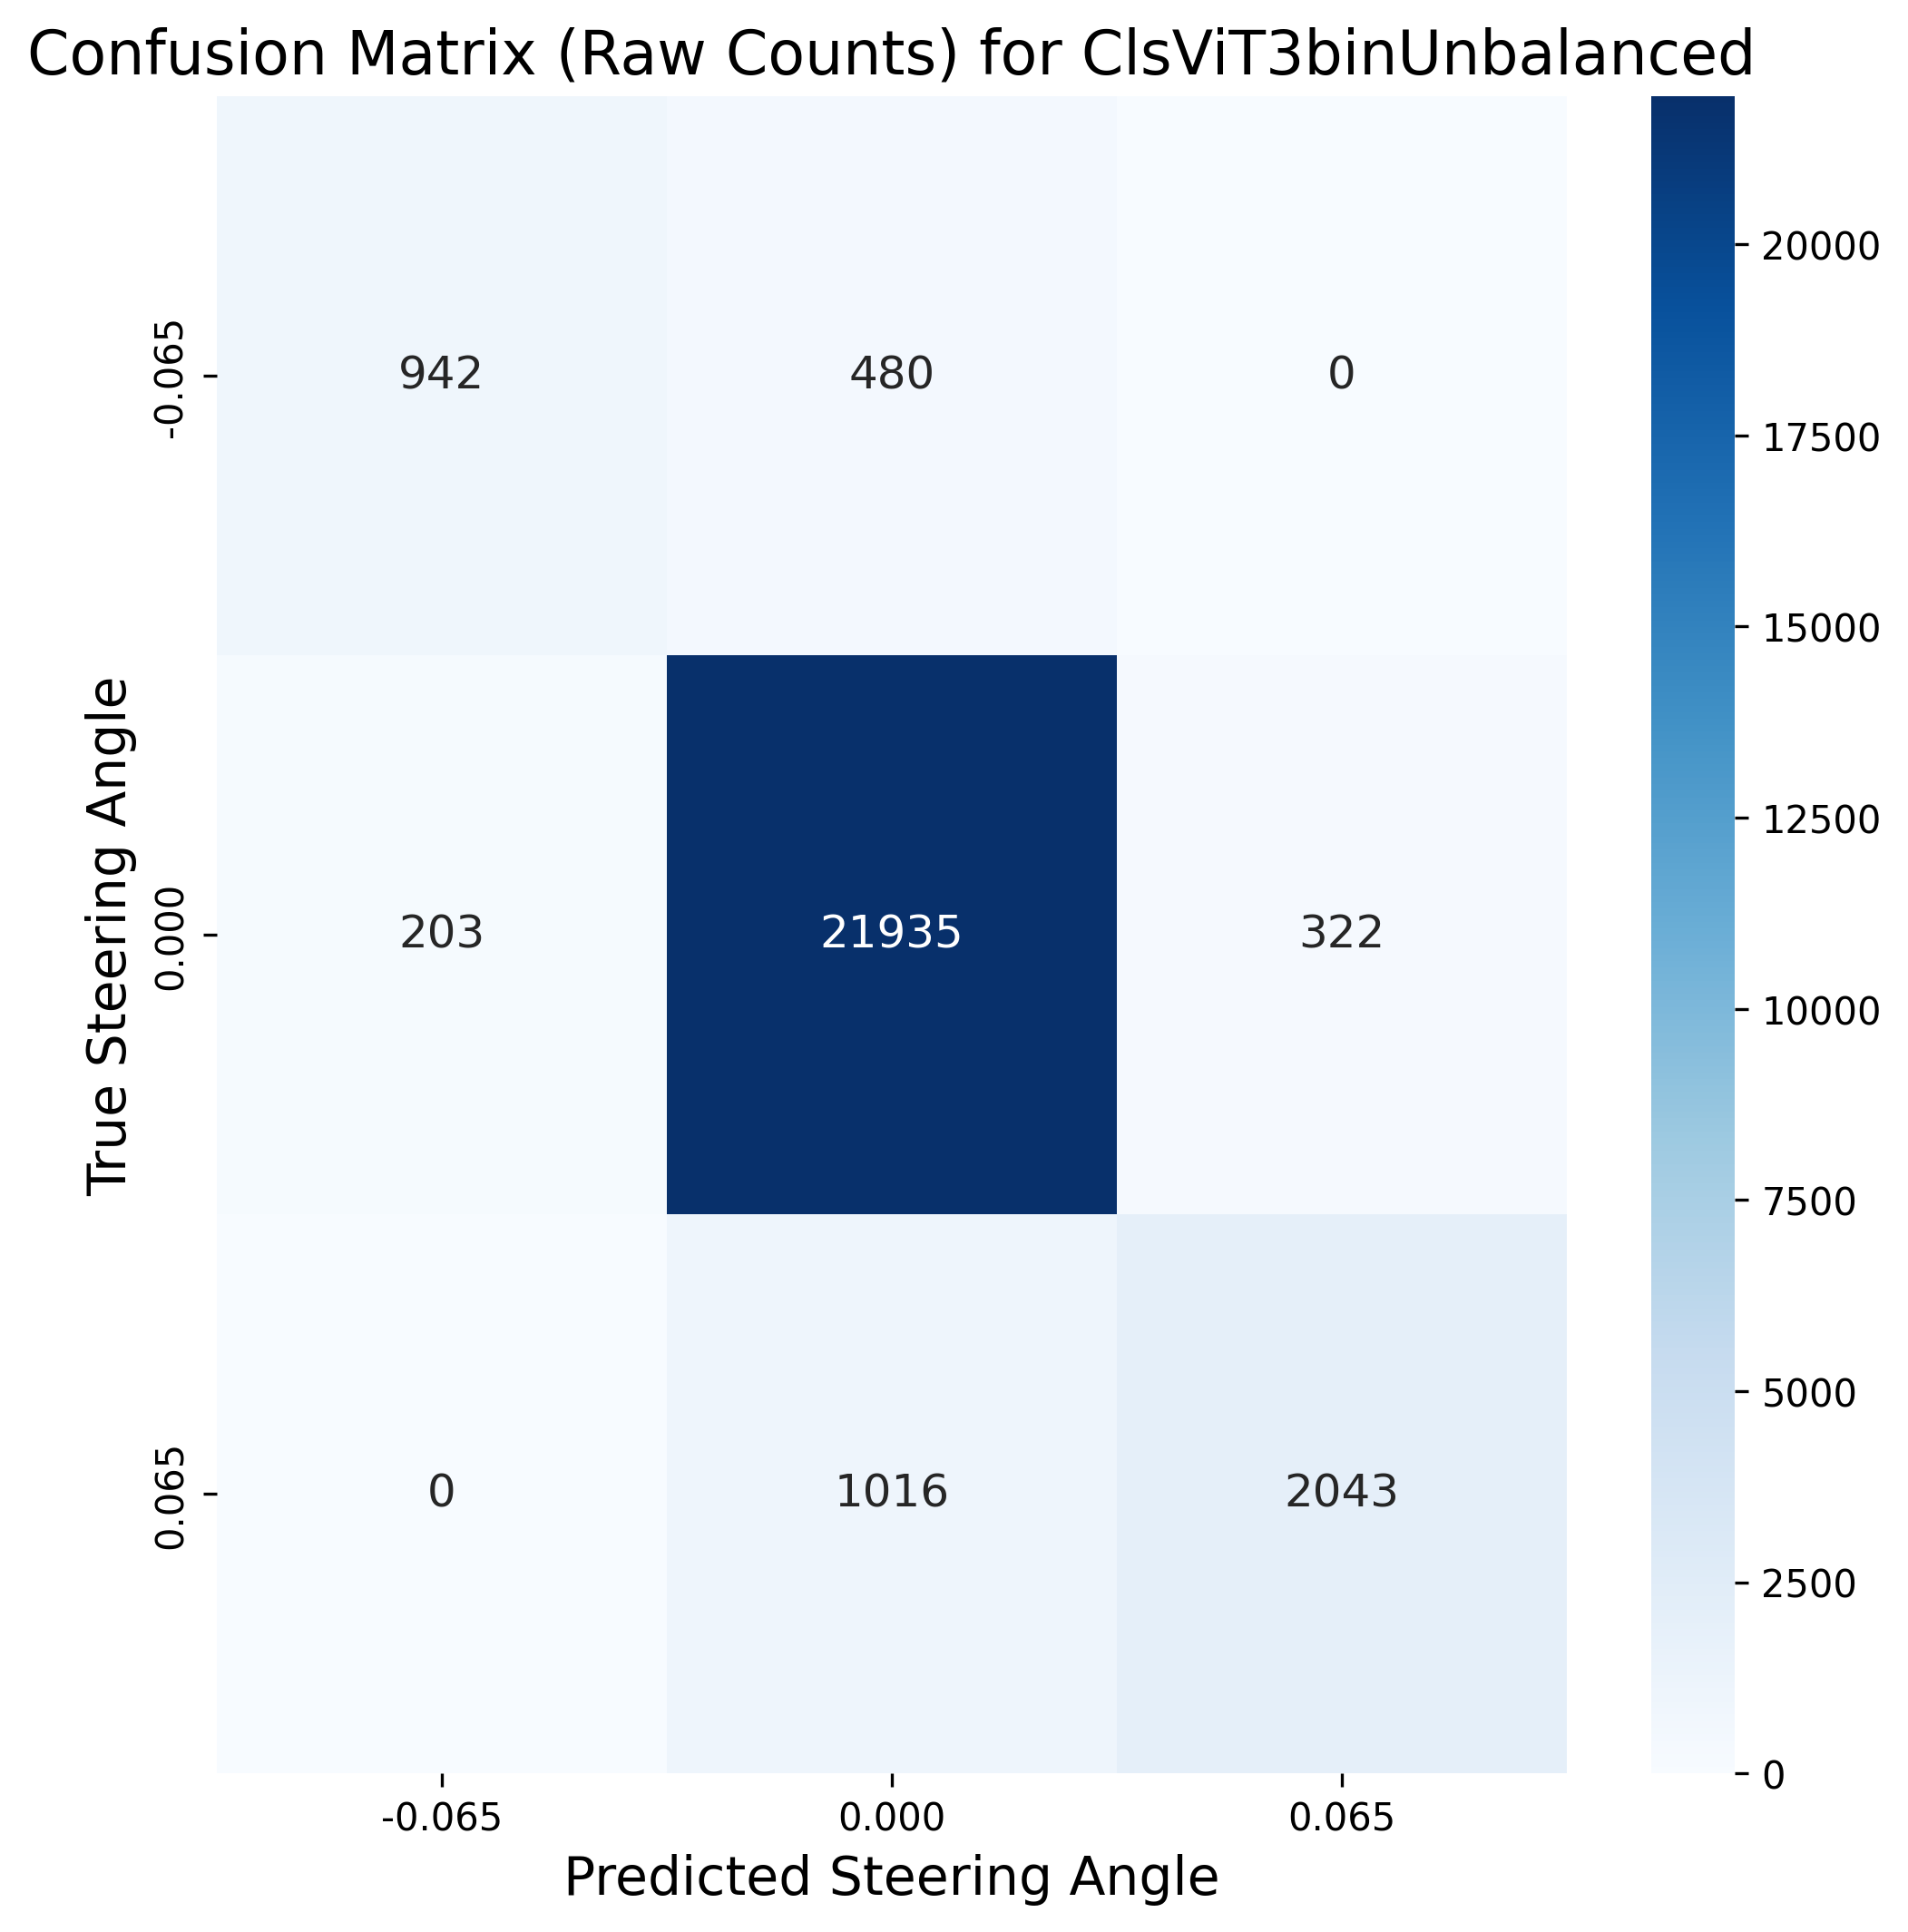
\includegraphics[width=0.65\linewidth]{Figures/Results/cm_raw_ClsViT3binUnbalanced.png}
\caption{ClsViT3binUnbalanced model raw counts confusion matrix}
\label{fig:cm_raw_ClsViT3binUnbalanced}
\end{figure}

\begin{figure}[H]
    \centering
    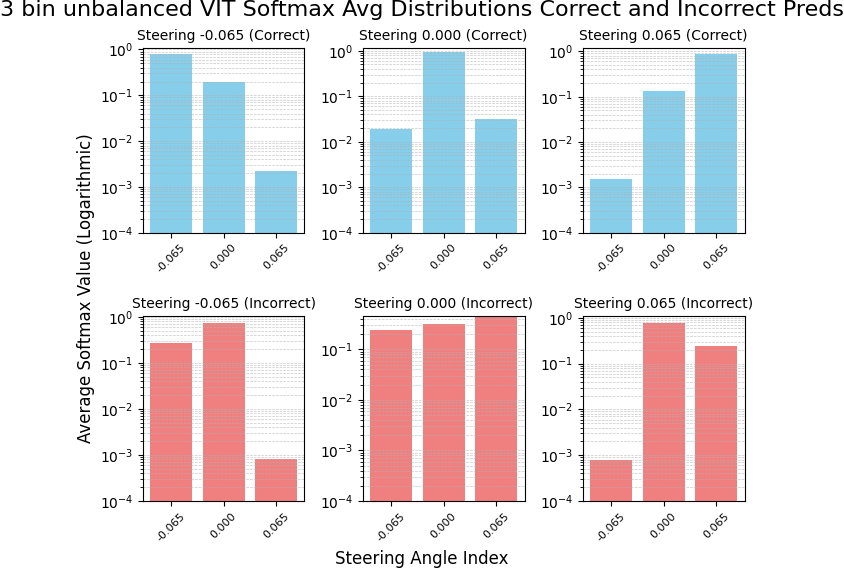
\includegraphics[width=1\linewidth]{Figures/Results/3_bins_vit_softmax_dist_plot_unbalanced.png}
    \caption{Average Softmax Probabilities for Correctly and Incorrectly Classified Steering Angles in the 3 bin vit unbalanced training Dataset.}
    \label{fig:3_bins_vit_softmax_dist_unbalanced}
\end{figure}

%%%%%%%%%%%%%%%%%%%%%%%%
% ClsViT5binUnbalanced %
%%%%%%%%%%%%%%%%%%%%%%%%

\subsubsection{ClsViT5binUnbalanced}

\begin{table}[htbp]
\centering
\begin{tabular}{@{}lcccc@{}}
\toprule
\textbf{Class} & \textbf{Precision} & \textbf{Recall} & \textbf{F1-Score} & \textbf{Support} \\
\midrule
$-0.065$ & 0.92 & 0.94 & 0.93 & 401 \\
$-0.015$ & 0.89 & 0.97 & 0.93 & 5,843 \\
$\phantom{-}0.000$ & 0.99 & 0.96 & 0.97 & 15,839 \\
$\phantom{-}0.015$ & 0.92 & 0.97 & 0.94 & 3,972 \\
$\phantom{-}0.065$ & 0.90 & 0.67 & 0.77 & 936 \\
\midrule
\textbf{Macro Avg} & \textbf{0.92} & \textbf{0.90} & \textbf{0.91} & \textbf{26,991} \\
\bottomrule
\end{tabular}
\caption{Classification performance results for the ClsViT5binUnbalanced model. The model achieved an overall accuracy of 94.97\% with a mean confidence of 0.9435 across 26,991 test images.}
\label{tab:clf_report_ClsViT5binUnbalanced}
\end{table}

\begin{figure}[H]
\centering
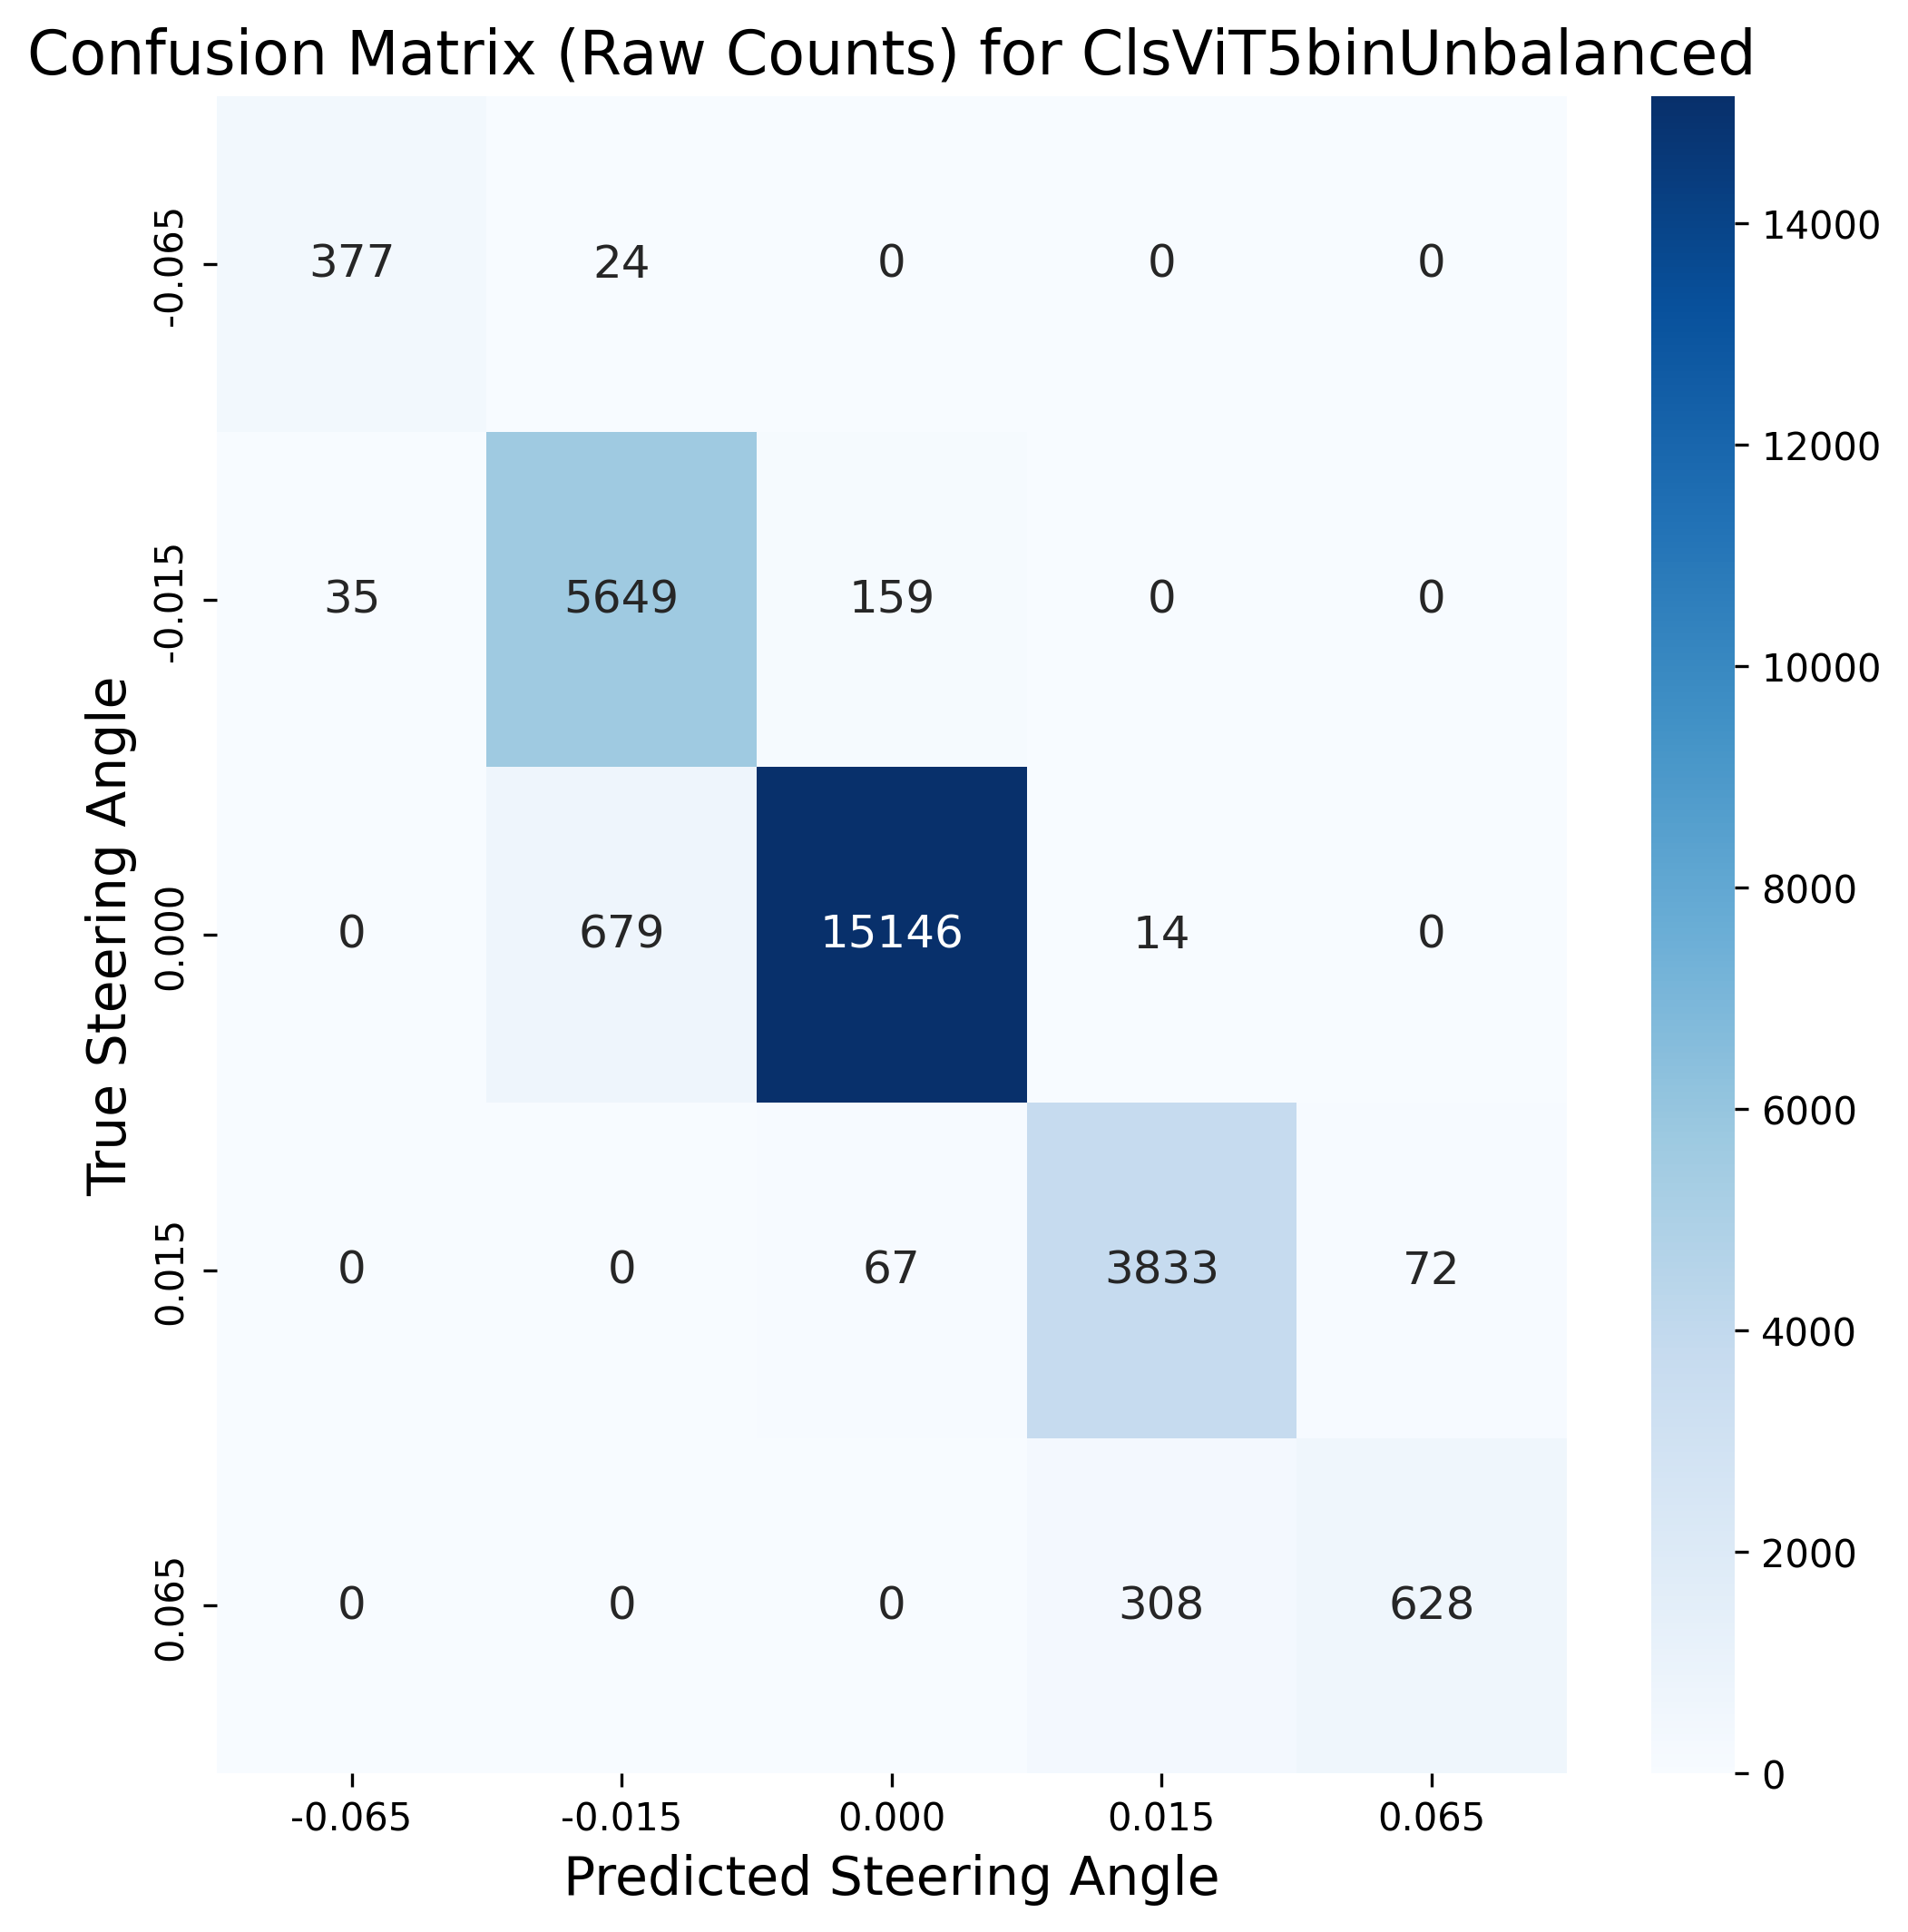
\includegraphics[width=0.65\linewidth]{Figures/Results/cm_raw_ClsViT5binUnbalanced.png}
\caption{ClsViT5binUnbalanced model raw counts confusion matrix}
\label{fig:cm_raw_ClsViT5binUnbalanced}
\end{figure}

\begin{figure}[H]
    \centering
    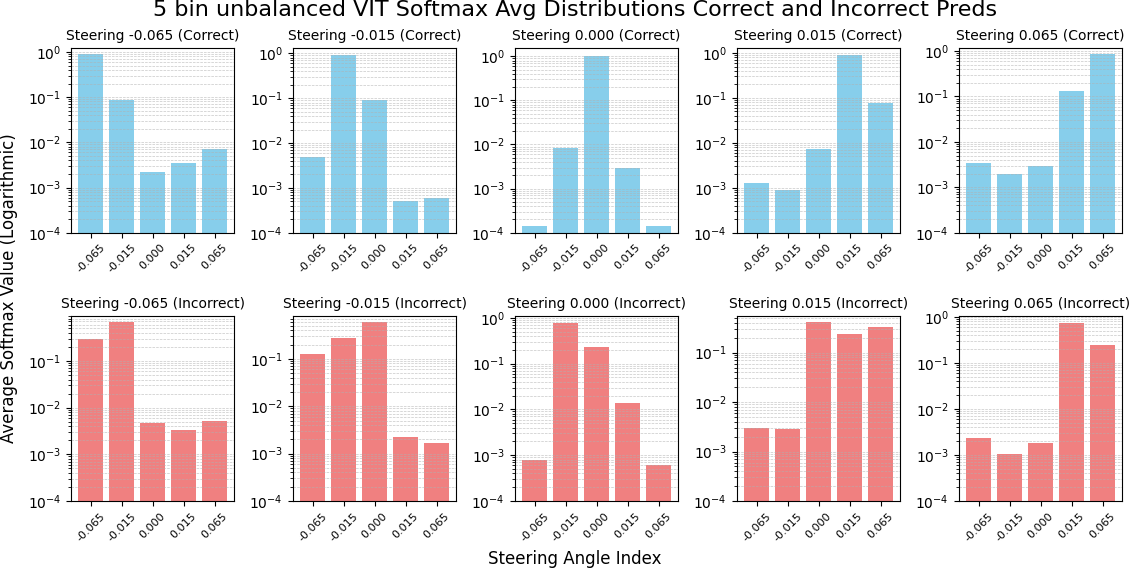
\includegraphics[width=1\linewidth]{Figures/Results/5_bins_vit_softmax_dist_plot_unbalanced.png}
    \caption{Average Softmax Probabilities for Correctly and Incorrectly Classified Steering Angles in the 5 bin vit unbalanced training Dataset.}
    \label{fig:5_bins_vit_softmax_dist_unbalanced}
\end{figure}

%%%%%%%%%%%%%%%%%%%%%%%
% ClsViT15binBalanced %
%%%%%%%%%%%%%%%%%%%%%%%

\subsubsection{ClsViT15binBalanced}

\begin{table}[htbp]
\centering
\begin{tabular}{@{}lcccc@{}}
\toprule
\textbf{Class} & \textbf{Precision} & \textbf{Recall} & \textbf{F1-Score} & \textbf{Support} \\
\midrule
$-0.065$ & 0.95 & 1.00 & 0.97 & 10,199 \\
$-0.055$ & 1.00 & 1.00 & 1.00 & 10,199 \\
$-0.045$ & 1.00 & 1.00 & 1.00 & 10,199 \\
$-0.035$ & 0.91 & 0.99 & 0.95 & 10,199 \\
$-0.025$ & 0.97 & 0.94 & 0.95 & 10,199 \\
$-0.015$ & 0.94 & 0.68 & 0.79 & 10,199 \\
$-0.005$ & 0.82 & 0.95 & 0.88 & 10,199 \\
$\phantom{-}0.000$ & 0.98 & 0.96 & 0.97 & 10,199 \\
$\phantom{-}0.005$ & 0.89 & 0.92 & 0.91 & 10,199 \\
$\phantom{-}0.015$ & 0.99 & 0.87 & 0.92 & 10,199 \\
$\phantom{-}0.025$ & 0.92 & 0.94 & 0.93 & 10,199 \\
$\phantom{-}0.035$ & 0.91 & 1.00 & 0.96 & 10,199 \\
$\phantom{-}0.045$ & 0.88 & 1.00 & 0.93 & 10,199 \\
$\phantom{-}0.055$ & 0.98 & 1.00 & 0.99 & 10,199 \\
$\phantom{-}0.065$ & 1.00 & 0.83 & 0.90 & 10,199 \\
\midrule
\textbf{Macro Avg} & \textbf{0.94} & \textbf{0.94} & \textbf{0.94} & \textbf{152,985} \\
\bottomrule
\end{tabular}
\caption{Classification performance results for the ClsViT15binBalanced model. The model achieved an overall accuracy of 93.86\% with a mean confidence of 0.9180 across 152,985 test images.}
\label{tab:clf_report_ClsViT15binBalanced}
\end{table}

\begin{figure}[H]
\centering
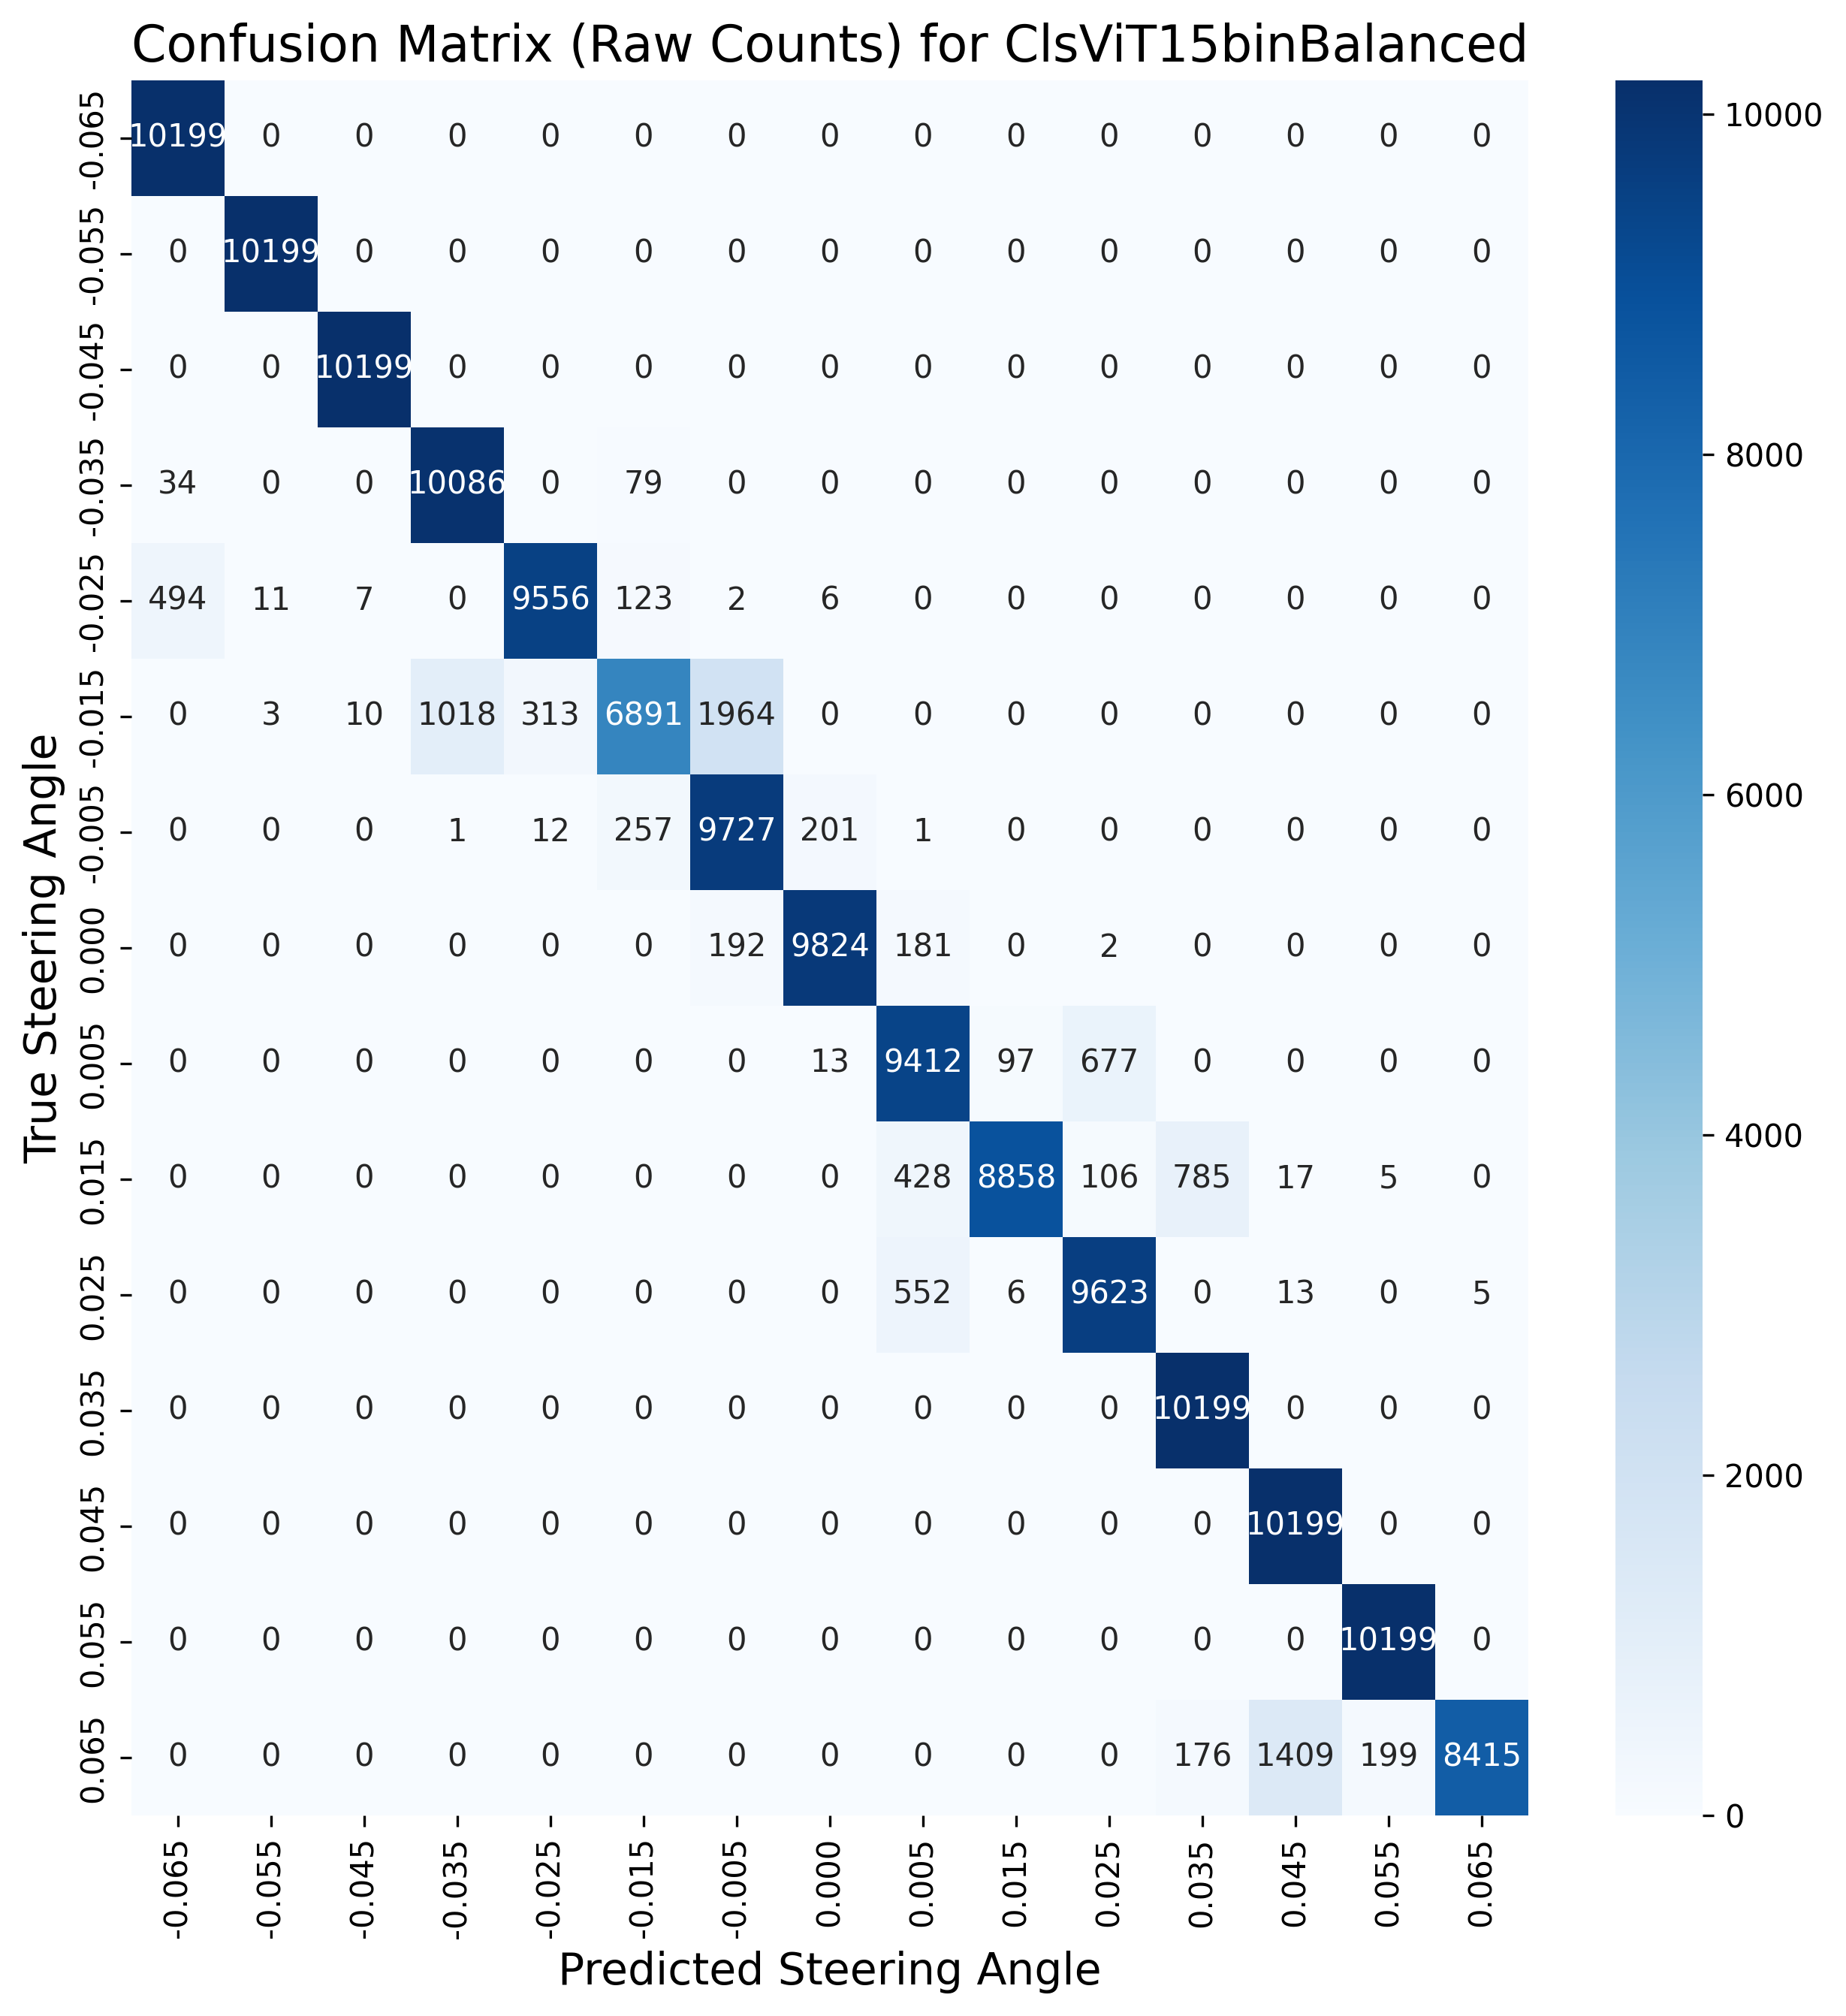
\includegraphics[width=1\linewidth]{Figures/Results/cm_raw_ClsViT15binBalanced.png}
\caption{ClsViT15binBalanced model raw counts confusion matrix}
\label{fig:cm_raw_ClsViT15binBalanced}
\end{figure}

\begin{figure}[H]
    \centering
    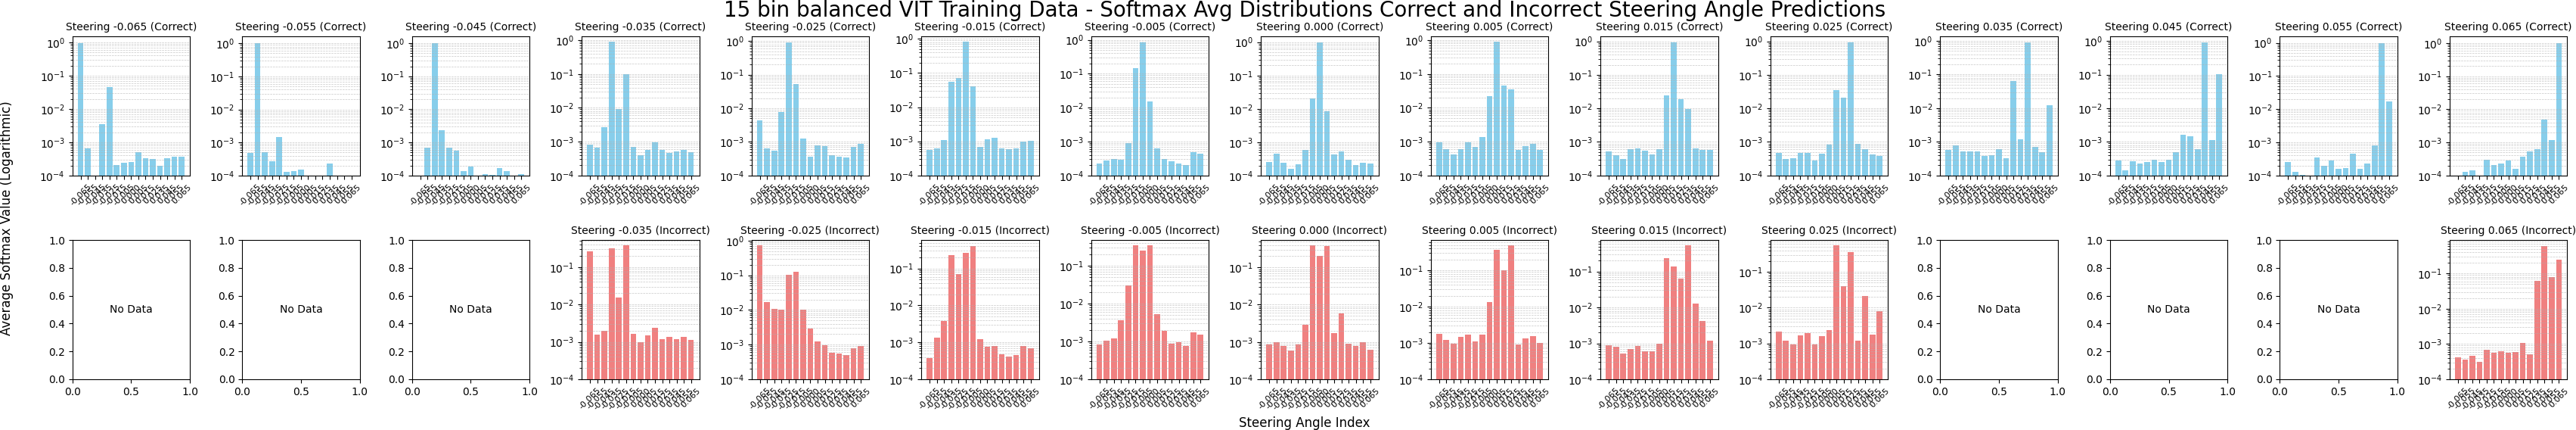
\includegraphics[width=1\linewidth]{Figures/Results/15_bins_vit_softmax_dist_plot_balanced.png}
    \caption{Average Softmax Probabilities for Correctly and Incorrectly Classified Steering Angles in the 15 bin vit balanced training Dataset.}
    \label{fig:15_bins_vit_softmax_dist_balanced}
\end{figure}

%%%%%%%%%%%%%%%%%%%%%%%%%
% ClsViT15binUnbalanced %
%%%%%%%%%%%%%%%%%%%%%%%%%

\subsubsection{ClsViT15binUnbalanced}

\begin{table}[htbp]
\centering
\begin{tabular}{@{}lcccc@{}}
\toprule
\textbf{Class} & \textbf{Precision} & \textbf{Recall} & \textbf{F1-Score} & \textbf{Support} \\
\midrule
$-0.065$ & 0.00 & 0.00 & 0.00 & 128 \\
$-0.055$ & 0.00 & 0.00 & 0.00 & 141 \\
$-0.045$ & 0.50 & 0.00 & 0.01 & 223 \\
$-0.035$ & 0.36 & 0.36 & 0.36 & 1,027 \\
$-0.025$ & 0.53 & 0.21 & 0.30 & 2,094 \\
$-0.015$ & 0.63 & 0.71 & 0.67 & 4,986 \\
$-0.005$ & 0.88 & 0.98 & 0.92 & 10,199 \\
$\phantom{-}0.000$ & 0.94 & 0.97 & 0.95 & 4,896 \\
$\phantom{-}0.005$ & 0.75 & 0.09 & 0.16 & 883 \\
$\phantom{-}0.015$ & 0.61 & 1.00 & 0.76 & 2,665 \\
$\phantom{-}0.025$ & 0.74 & 0.02 & 0.05 & 827 \\
$\phantom{-}0.035$ & 0.00 & 0.00 & 0.00 & 240 \\
$\phantom{-}0.045$ & 0.36 & 0.08 & 0.13 & 124 \\
$\phantom{-}0.055$ & 0.54 & 0.05 & 0.09 & 150 \\
$\phantom{-}0.065$ & 0.61 & 0.98 & 0.76 & 408 \\
\midrule
\textbf{Macro Avg} & \textbf{0.50} & \textbf{0.36} & \textbf{0.34} & \textbf{28,991} \\
\bottomrule
\end{tabular}
\caption{Classification performance results for the ClsViT15binUnbalanced model. The model achieved an overall accuracy of 76.55\% with a mean confidence of 0.7572 across 28,991 test images.}
\label{tab:clf_report_ClsViT15binUnbalanced}
\end{table}

\begin{figure}[H]
\centering
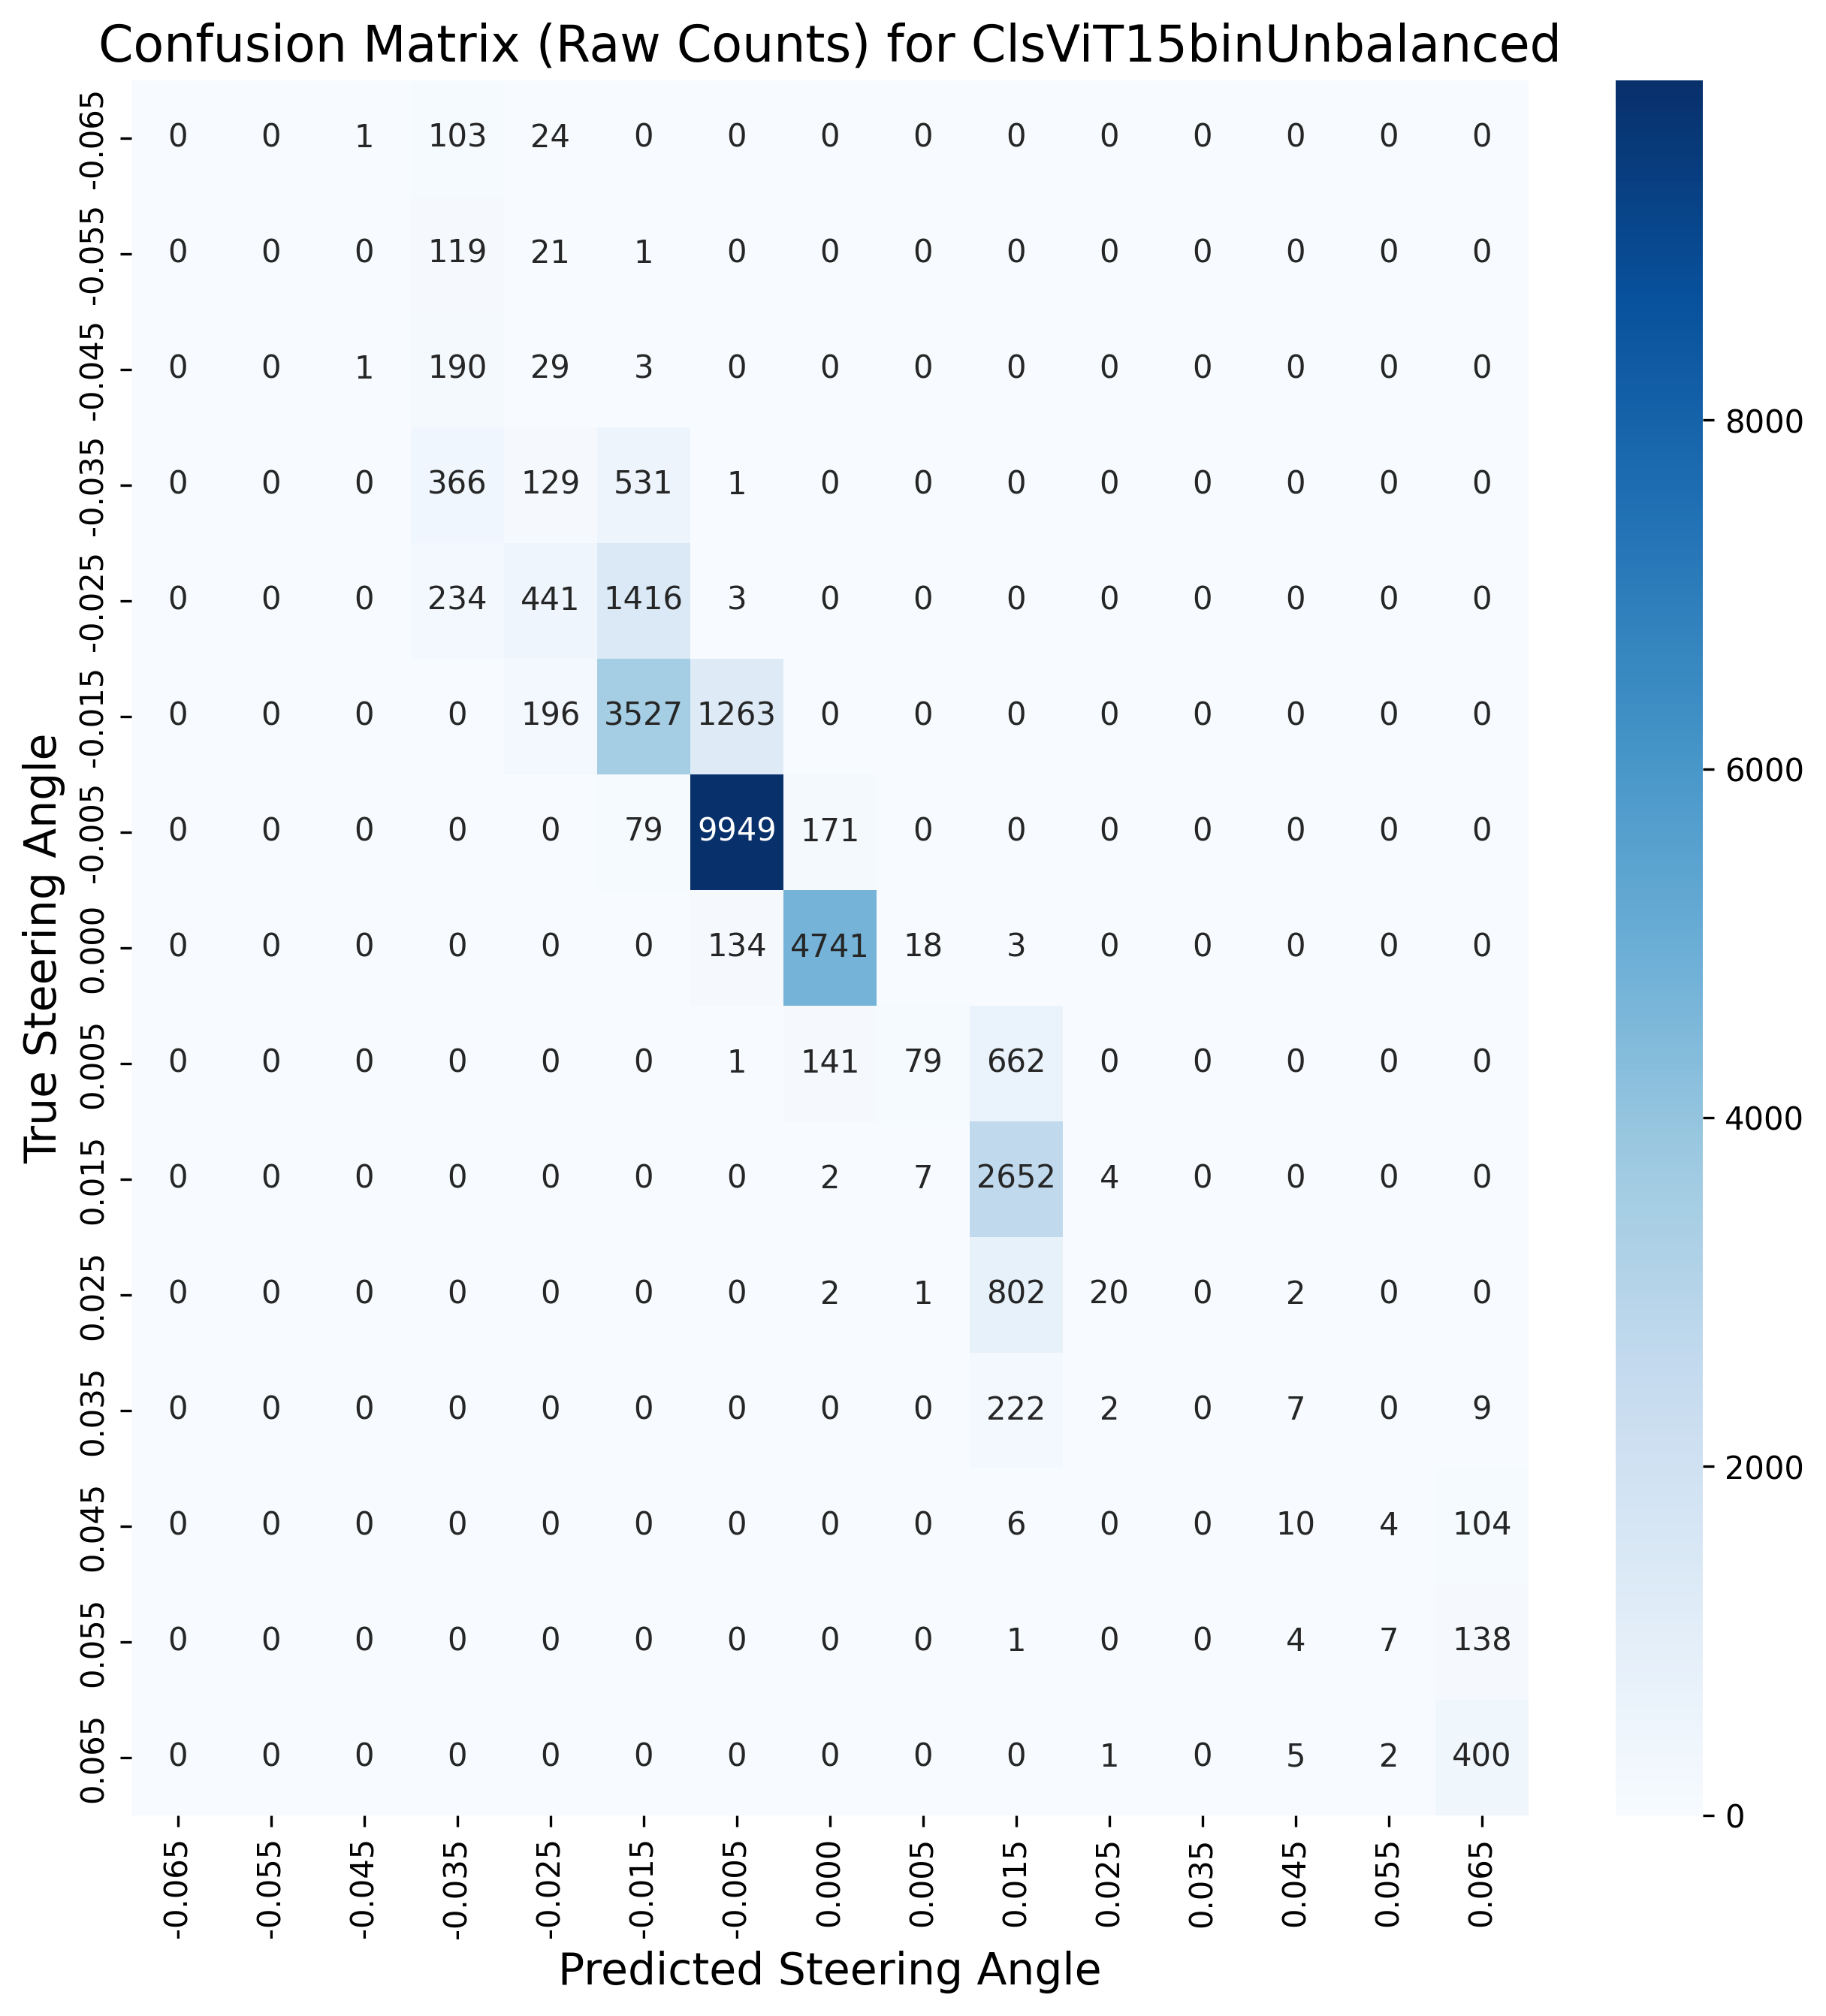
\includegraphics[width=1\linewidth]{Figures/Results/cm_raw_ClsViT15binUnbalanced.png}
\caption{ClsViT15binUnbalanced model raw counts confusion matrix}
\label{fig:cm_raw_ClsViT15binUnbalanced}
\end{figure}

\begin{figure}[H]
    \centering
    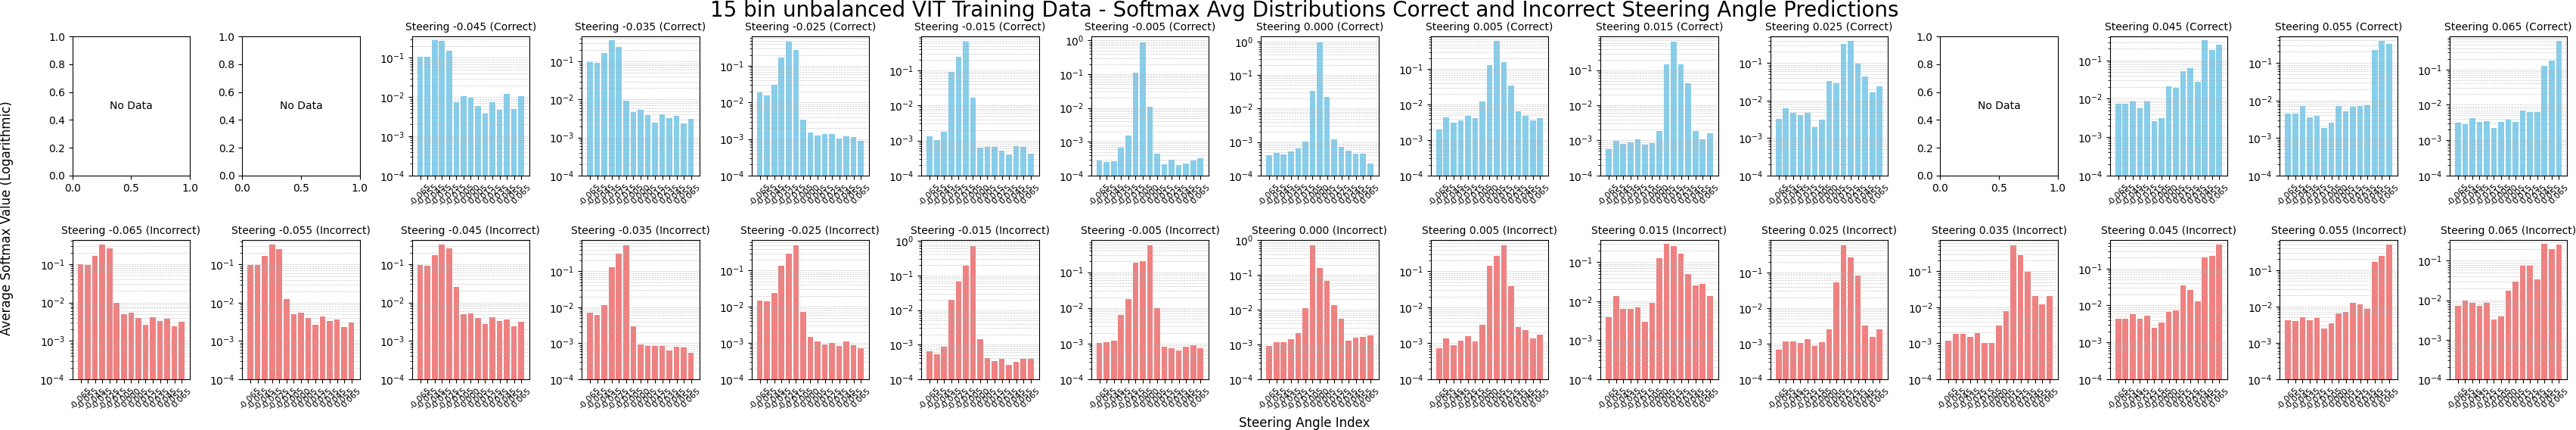
\includegraphics[width=1\linewidth]{Figures/Results/15_bins_vit_softmax_dist_plot_unbalanced.png}
    \caption{Average Softmax Probabilities for Correctly and Incorrectly Classified Steering Angles in the 15 bin vit unbalanced training Dataset.}
    \label{fig:15_bins_vit_softmax_dist_unbalanced}
\end{figure}

%%%%%%%%%%%%%%%%%%%%%%%%
% ClsVLM3binUnbalanced %
%%%%%%%%%%%%%%%%%%%%%%%%

\subsubsection{ClsVLM3binUnbalanced}

\begin{table}[htbp]
\centering
\begin{tabular}{@{}lcccc@{}}
\toprule
\textbf{Class} & \textbf{Precision} & \textbf{Recall} & \textbf{F1-Score} & \textbf{Support} \\
\midrule
$-0.065$ & 0.50 & 0.19 & 0.27 & 1,422 \\
$\phantom{-}0.000$ & 0.86 & 0.99 & 0.92 & 22,460 \\
$\phantom{-}0.065$ & 0.91 & 0.17 & 0.28 & 3,059 \\
\midrule
\textbf{Macro Avg} & \textbf{0.76} & \textbf{0.45} & \textbf{0.49} & \textbf{26,941} \\
\bottomrule
\end{tabular}
\caption{Classification performance results for the ClsVLM3binUnbalanced model. The model achieved an overall accuracy of 85.08\% with a mean confidence of 0.9062 across 26,941 test images.}
\label{tab:clf_report_ClsVLM3binUnbalanced}
\end{table}

\begin{figure}[H]
\centering
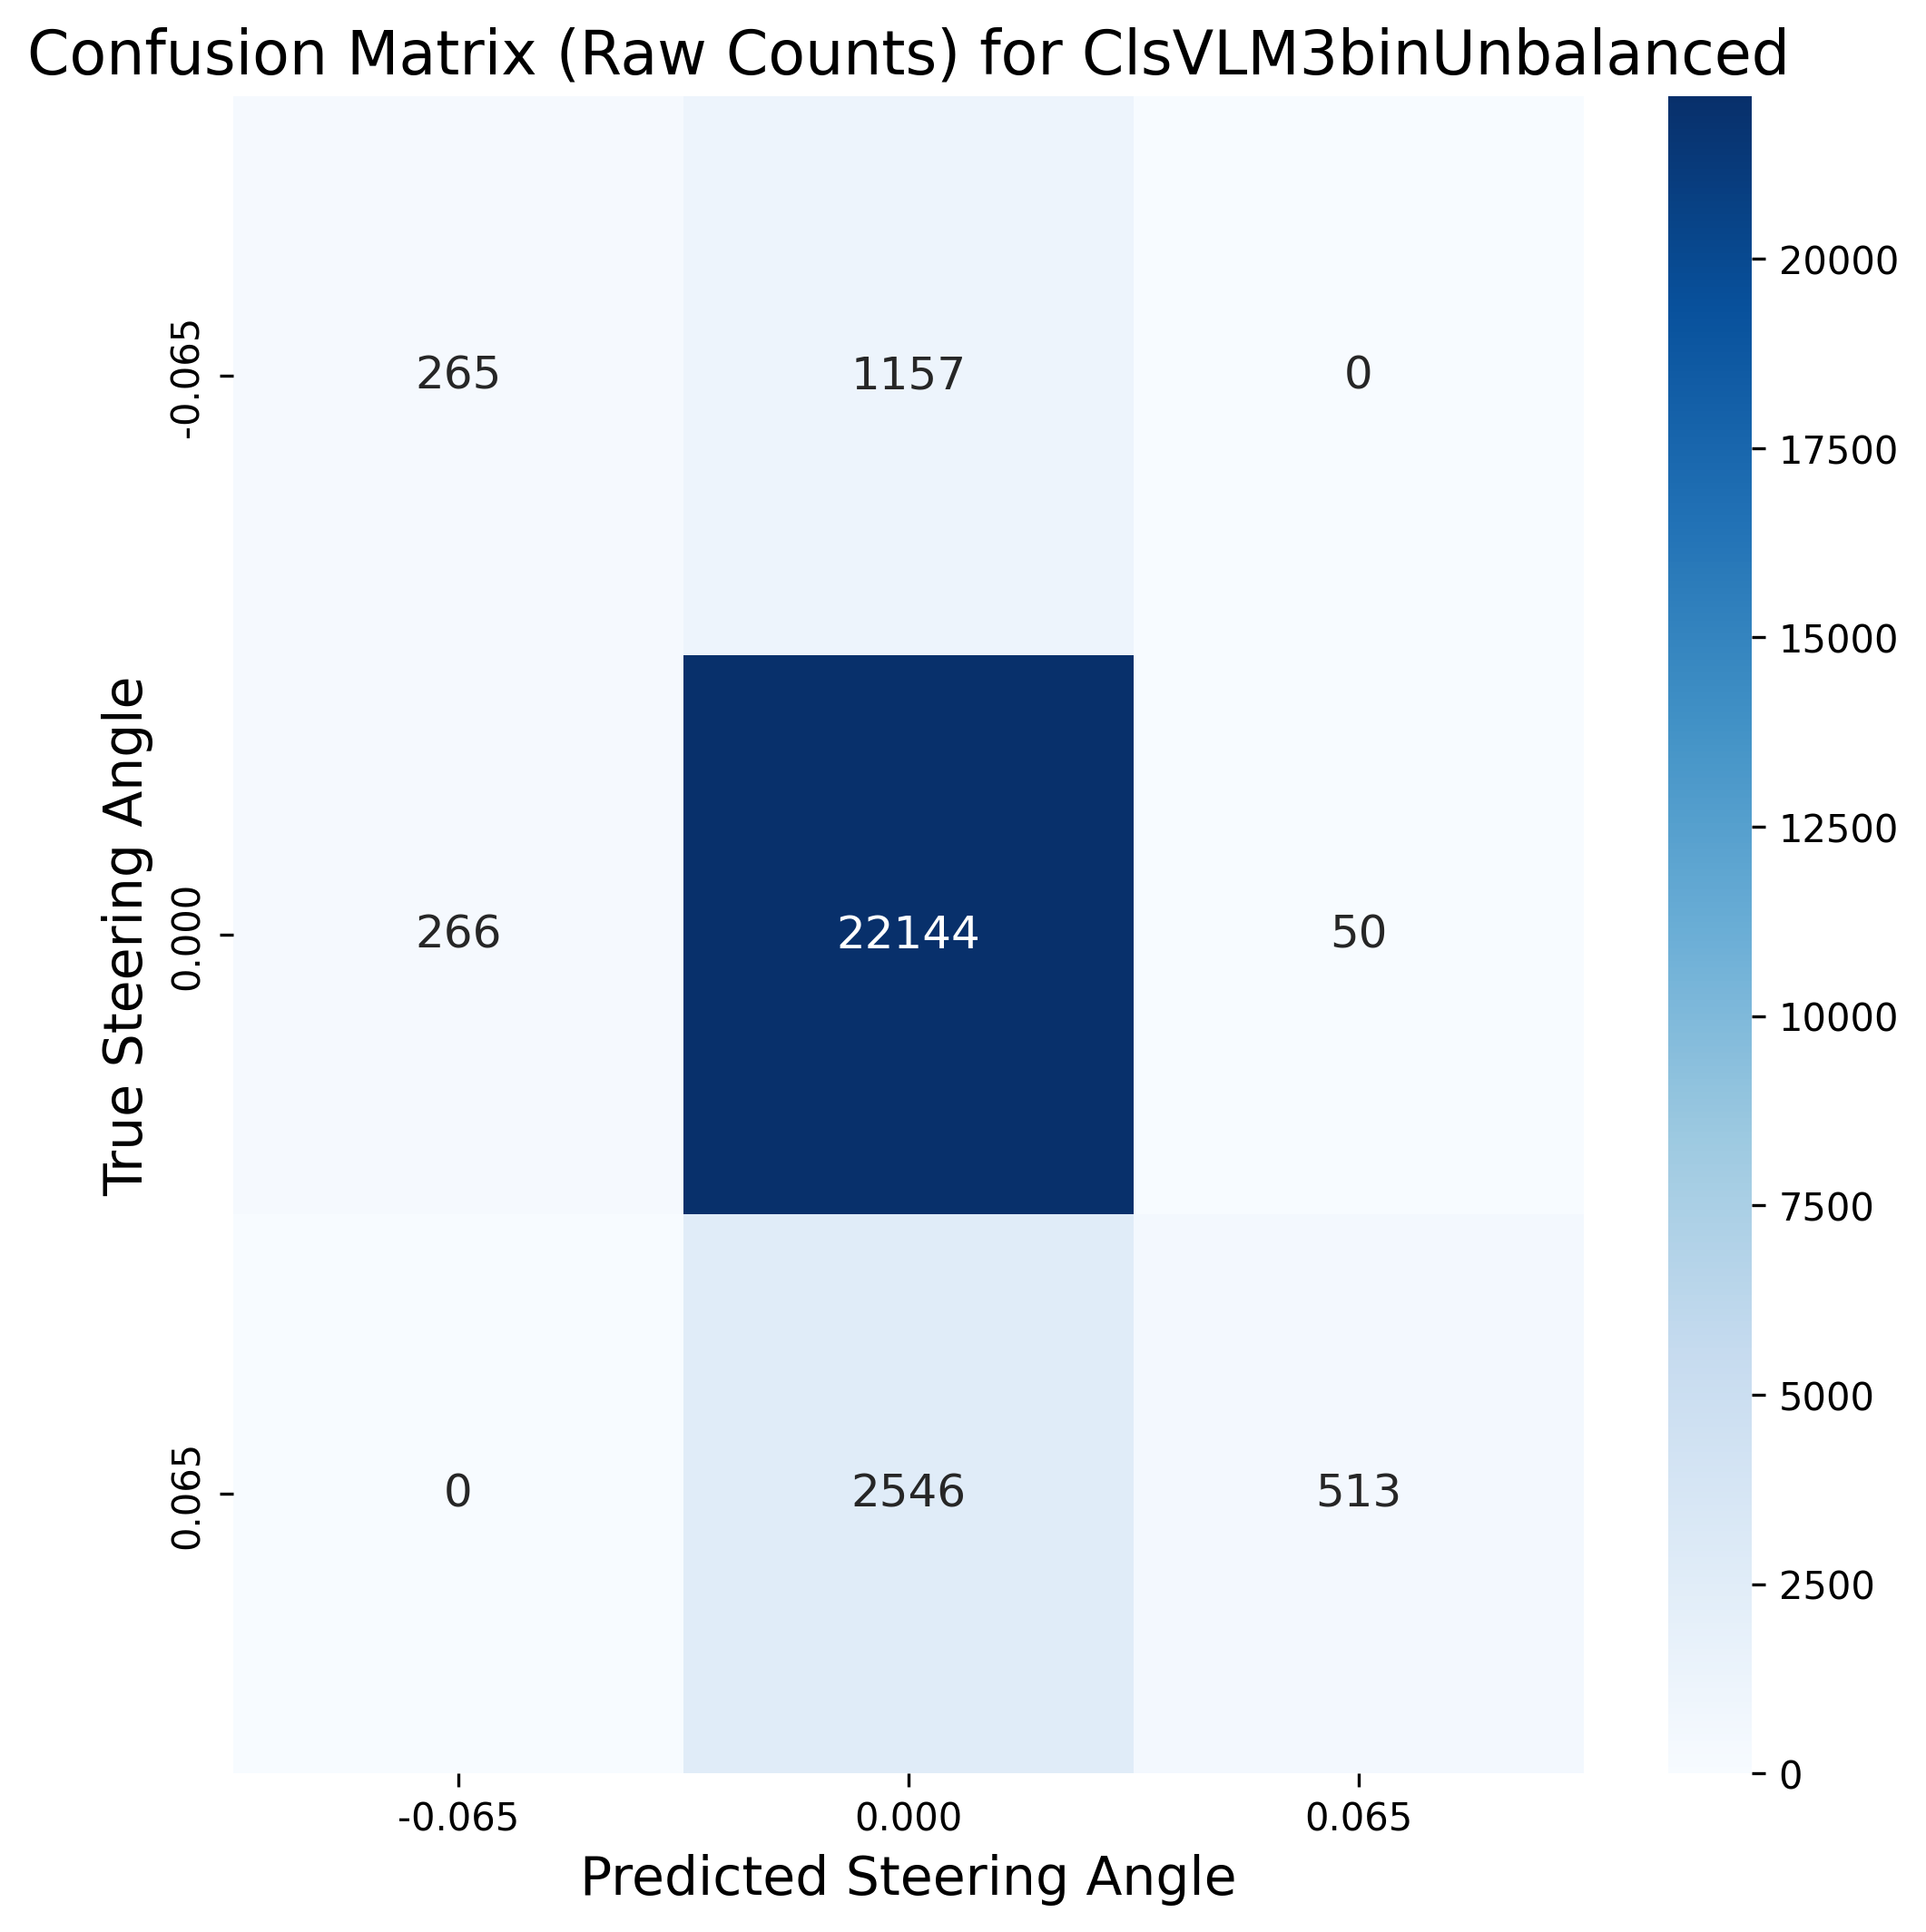
\includegraphics[width=0.65\linewidth]{Figures/Results/cm_raw_ClsVLM3binUnbalanced.png}
\caption{ClsVLM3binUnbalanced model raw counts confusion matrix}
\label{fig:cm_raw_ClsVLM3binUnbalanced}
\end{figure}

\begin{figure}[H]
    \centering
    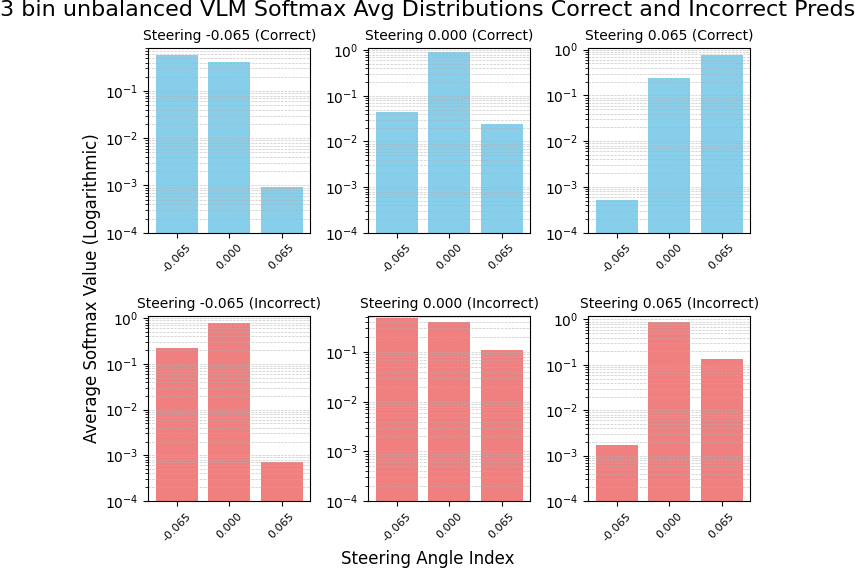
\includegraphics[width=1\linewidth]{Figures/Results/3_bins_vlm_softmax_dist_plot_unbalanced.png}
    \caption{Average Softmax Probabilities for Correctly and Incorrectly Classified Steering Angles in the 3 bin vlm unbalanced training Dataset.}
    \label{fig:3_bins_vlm_softmax_dist_unbalanced}
\end{figure}



%%%%%%%%%%%%%%%%%%%%%%%%%%%%%%%%%%
% ANALYSIS OF CLASSIFIER OUTPUTS %
%%%%%%%%%%%%%%%%%%%%%%%%%%%%%%%%%%

% \subsection{Analysis of Classifier Outputs}

% %%%%%%%%%%%%%%%%%%%%%%
% % ClsCNN3binBalanced %
% %%%%%%%%%%%%%%%%%%%%%%

% \begin{table}[htbp]
% \centering
% \begin{tabular}{@{}lcccc@{}}
% \toprule
% \textbf{Class} & \textbf{Precision} & \textbf{Recall} & \textbf{F1-Score} & \textbf{Support} \\
% \midrule
% $-0.065$ & 0.88 & 0.95 & 0.91 & 22,460 \\
% $\phantom{-}0.000$ & 0.80 & 0.66 & 0.73 & 22,460 \\
% $\phantom{-}0.065$ & 0.81 & 0.89 & 0.85 & 22,460 \\
% \midrule
% \textbf{Macro Avg} & \textbf{0.83} & \textbf{0.83} & \textbf{0.83} & \textbf{67,380} \\
% \bottomrule
% \end{tabular}
% \caption{Classification performance results for the ClsCNN3binBalanced model. The model achieved an overall accuracy of 83.36\% with a mean confidence of 0.8312 across 67,380 test images.}
% \label{tab:clf_report_ClsCNN3binBalanced}
% \end{table}

% % ClsCNN3binBalanced Raw Counts Confusion Matrix %

% \begin{figure}[H]
% \centering
% 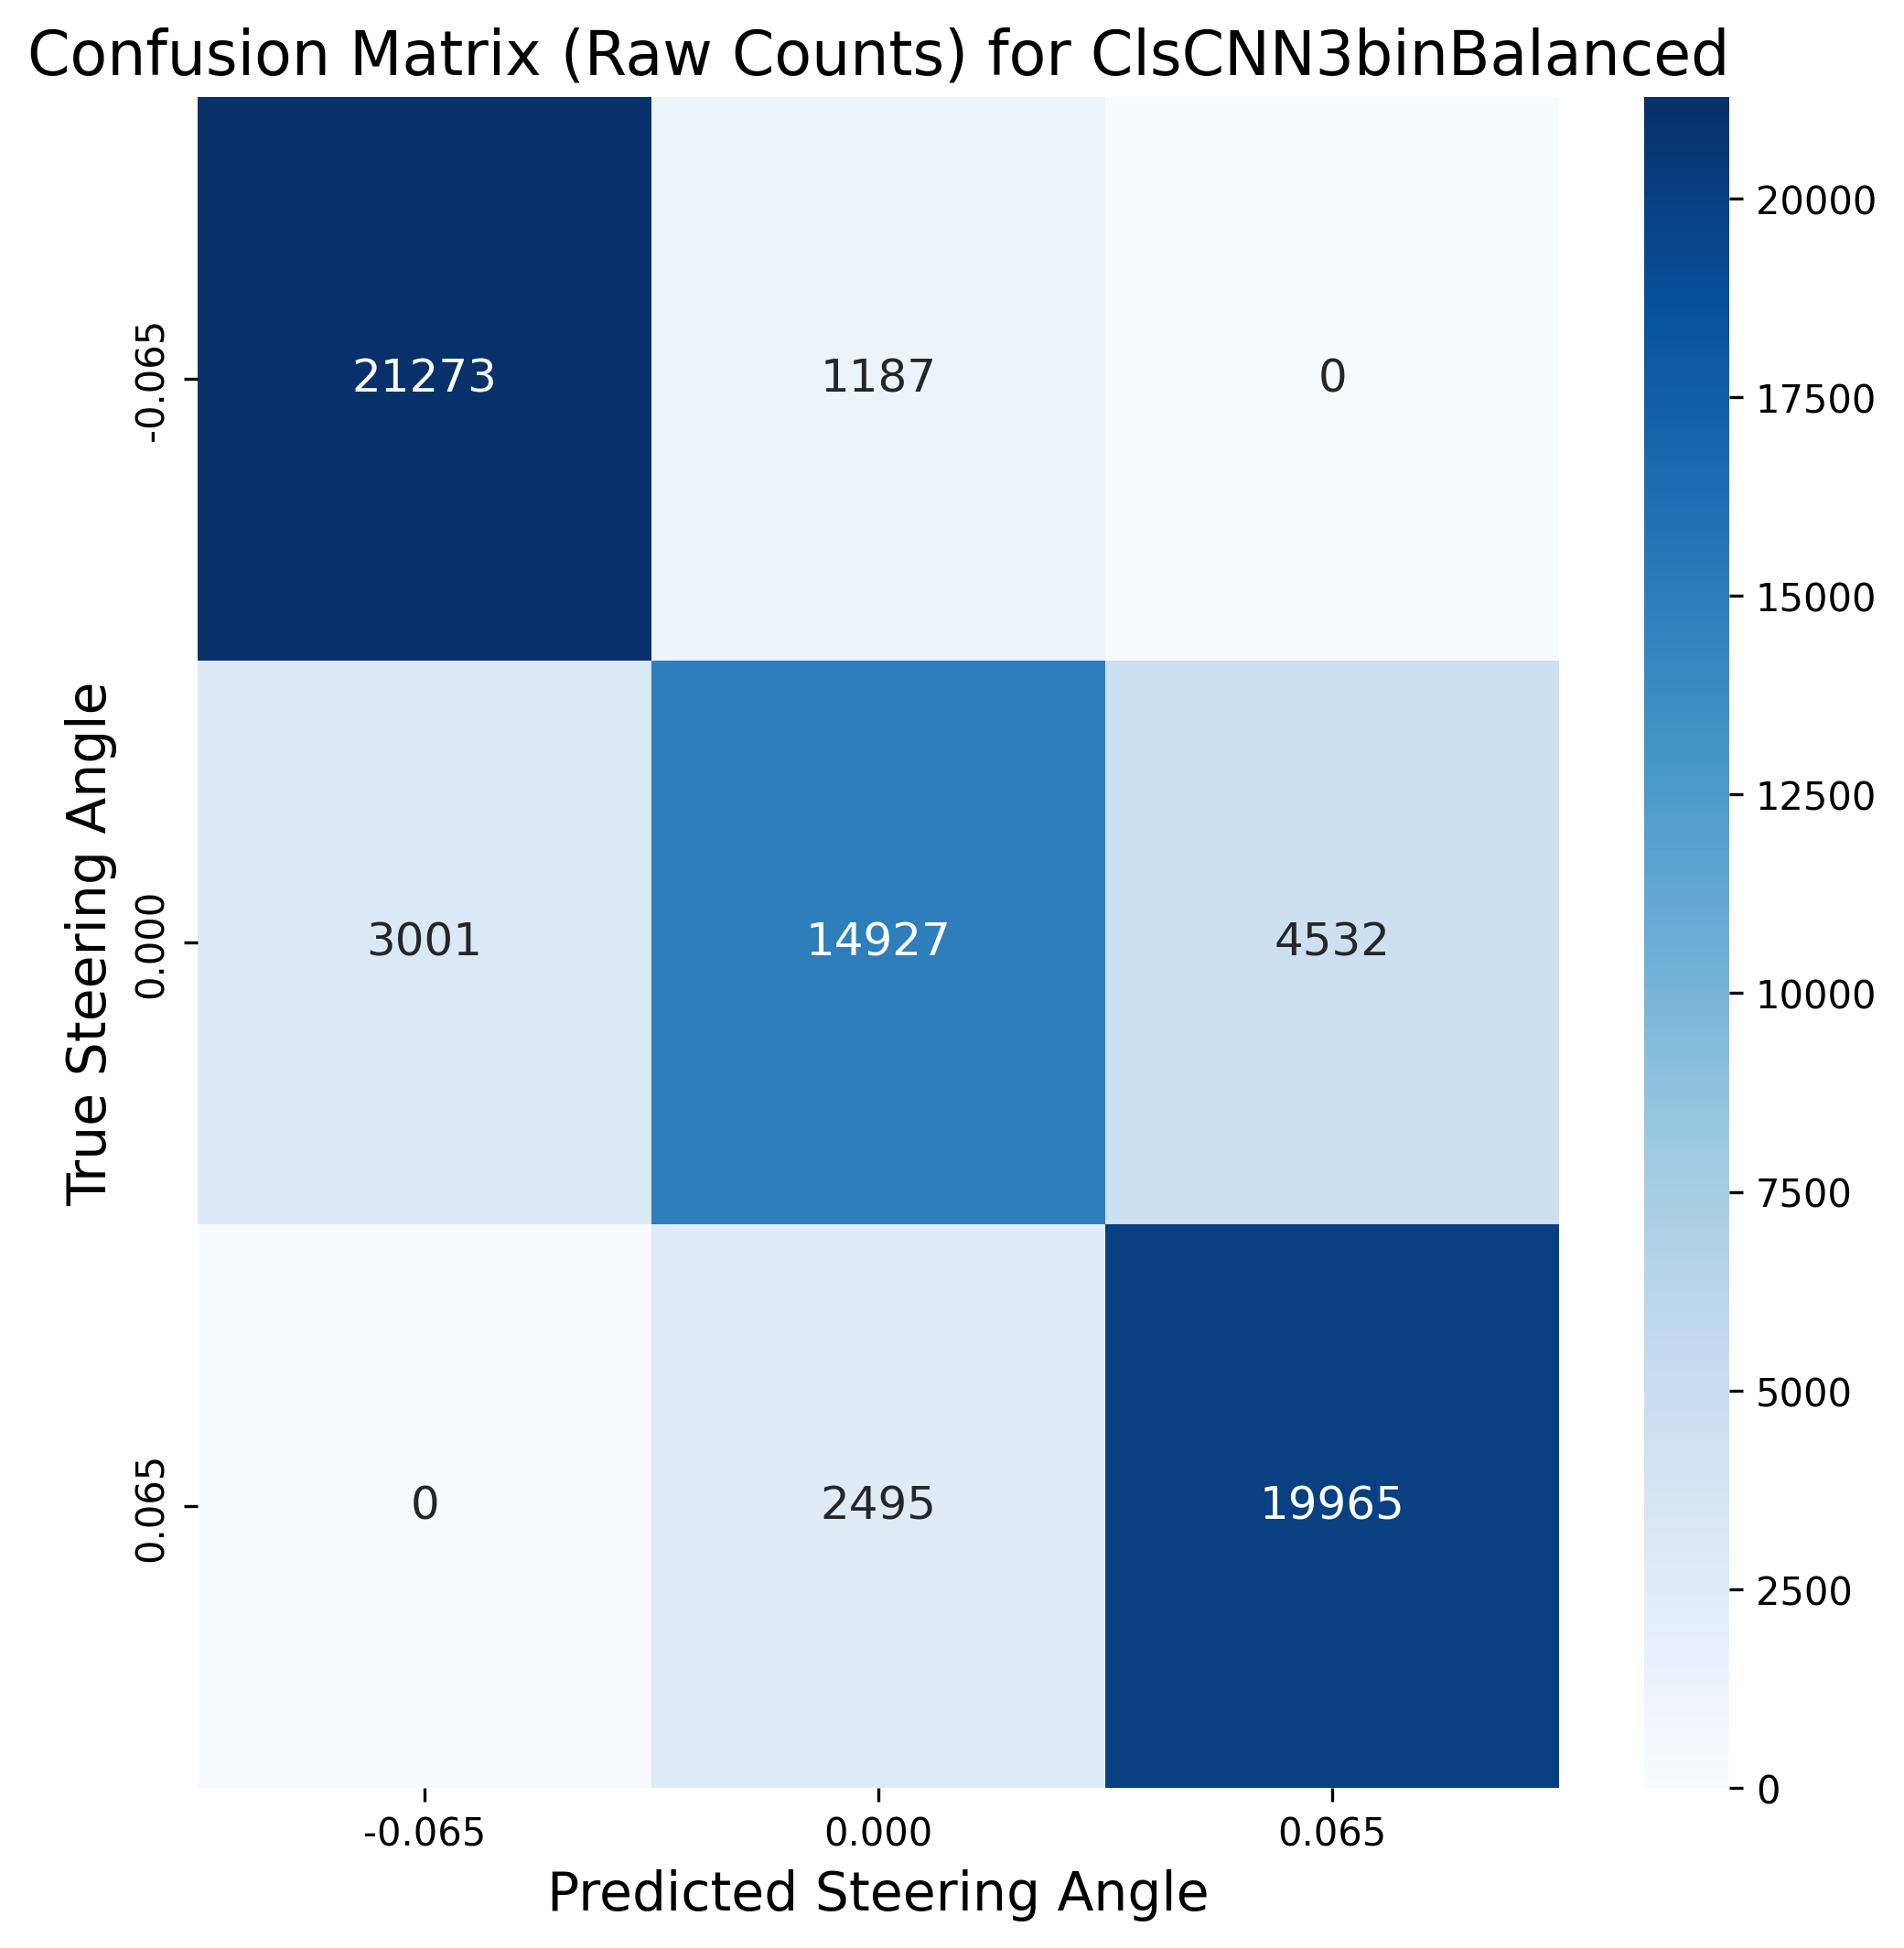
\includegraphics[width=0.65\linewidth]{Figures/Results/cm_raw_ClsCNN3binBalanced.png}
% \caption{ClsCNN3binBalanced model raw counts confusion matrix}
% \label{fig:cm_raw_ClsCNN3binBalanced}
% \end{figure}

% % ClsCNN3binBalanced Normalized Confusion Matrix %

% \begin{figure}[H]
% \centering
% 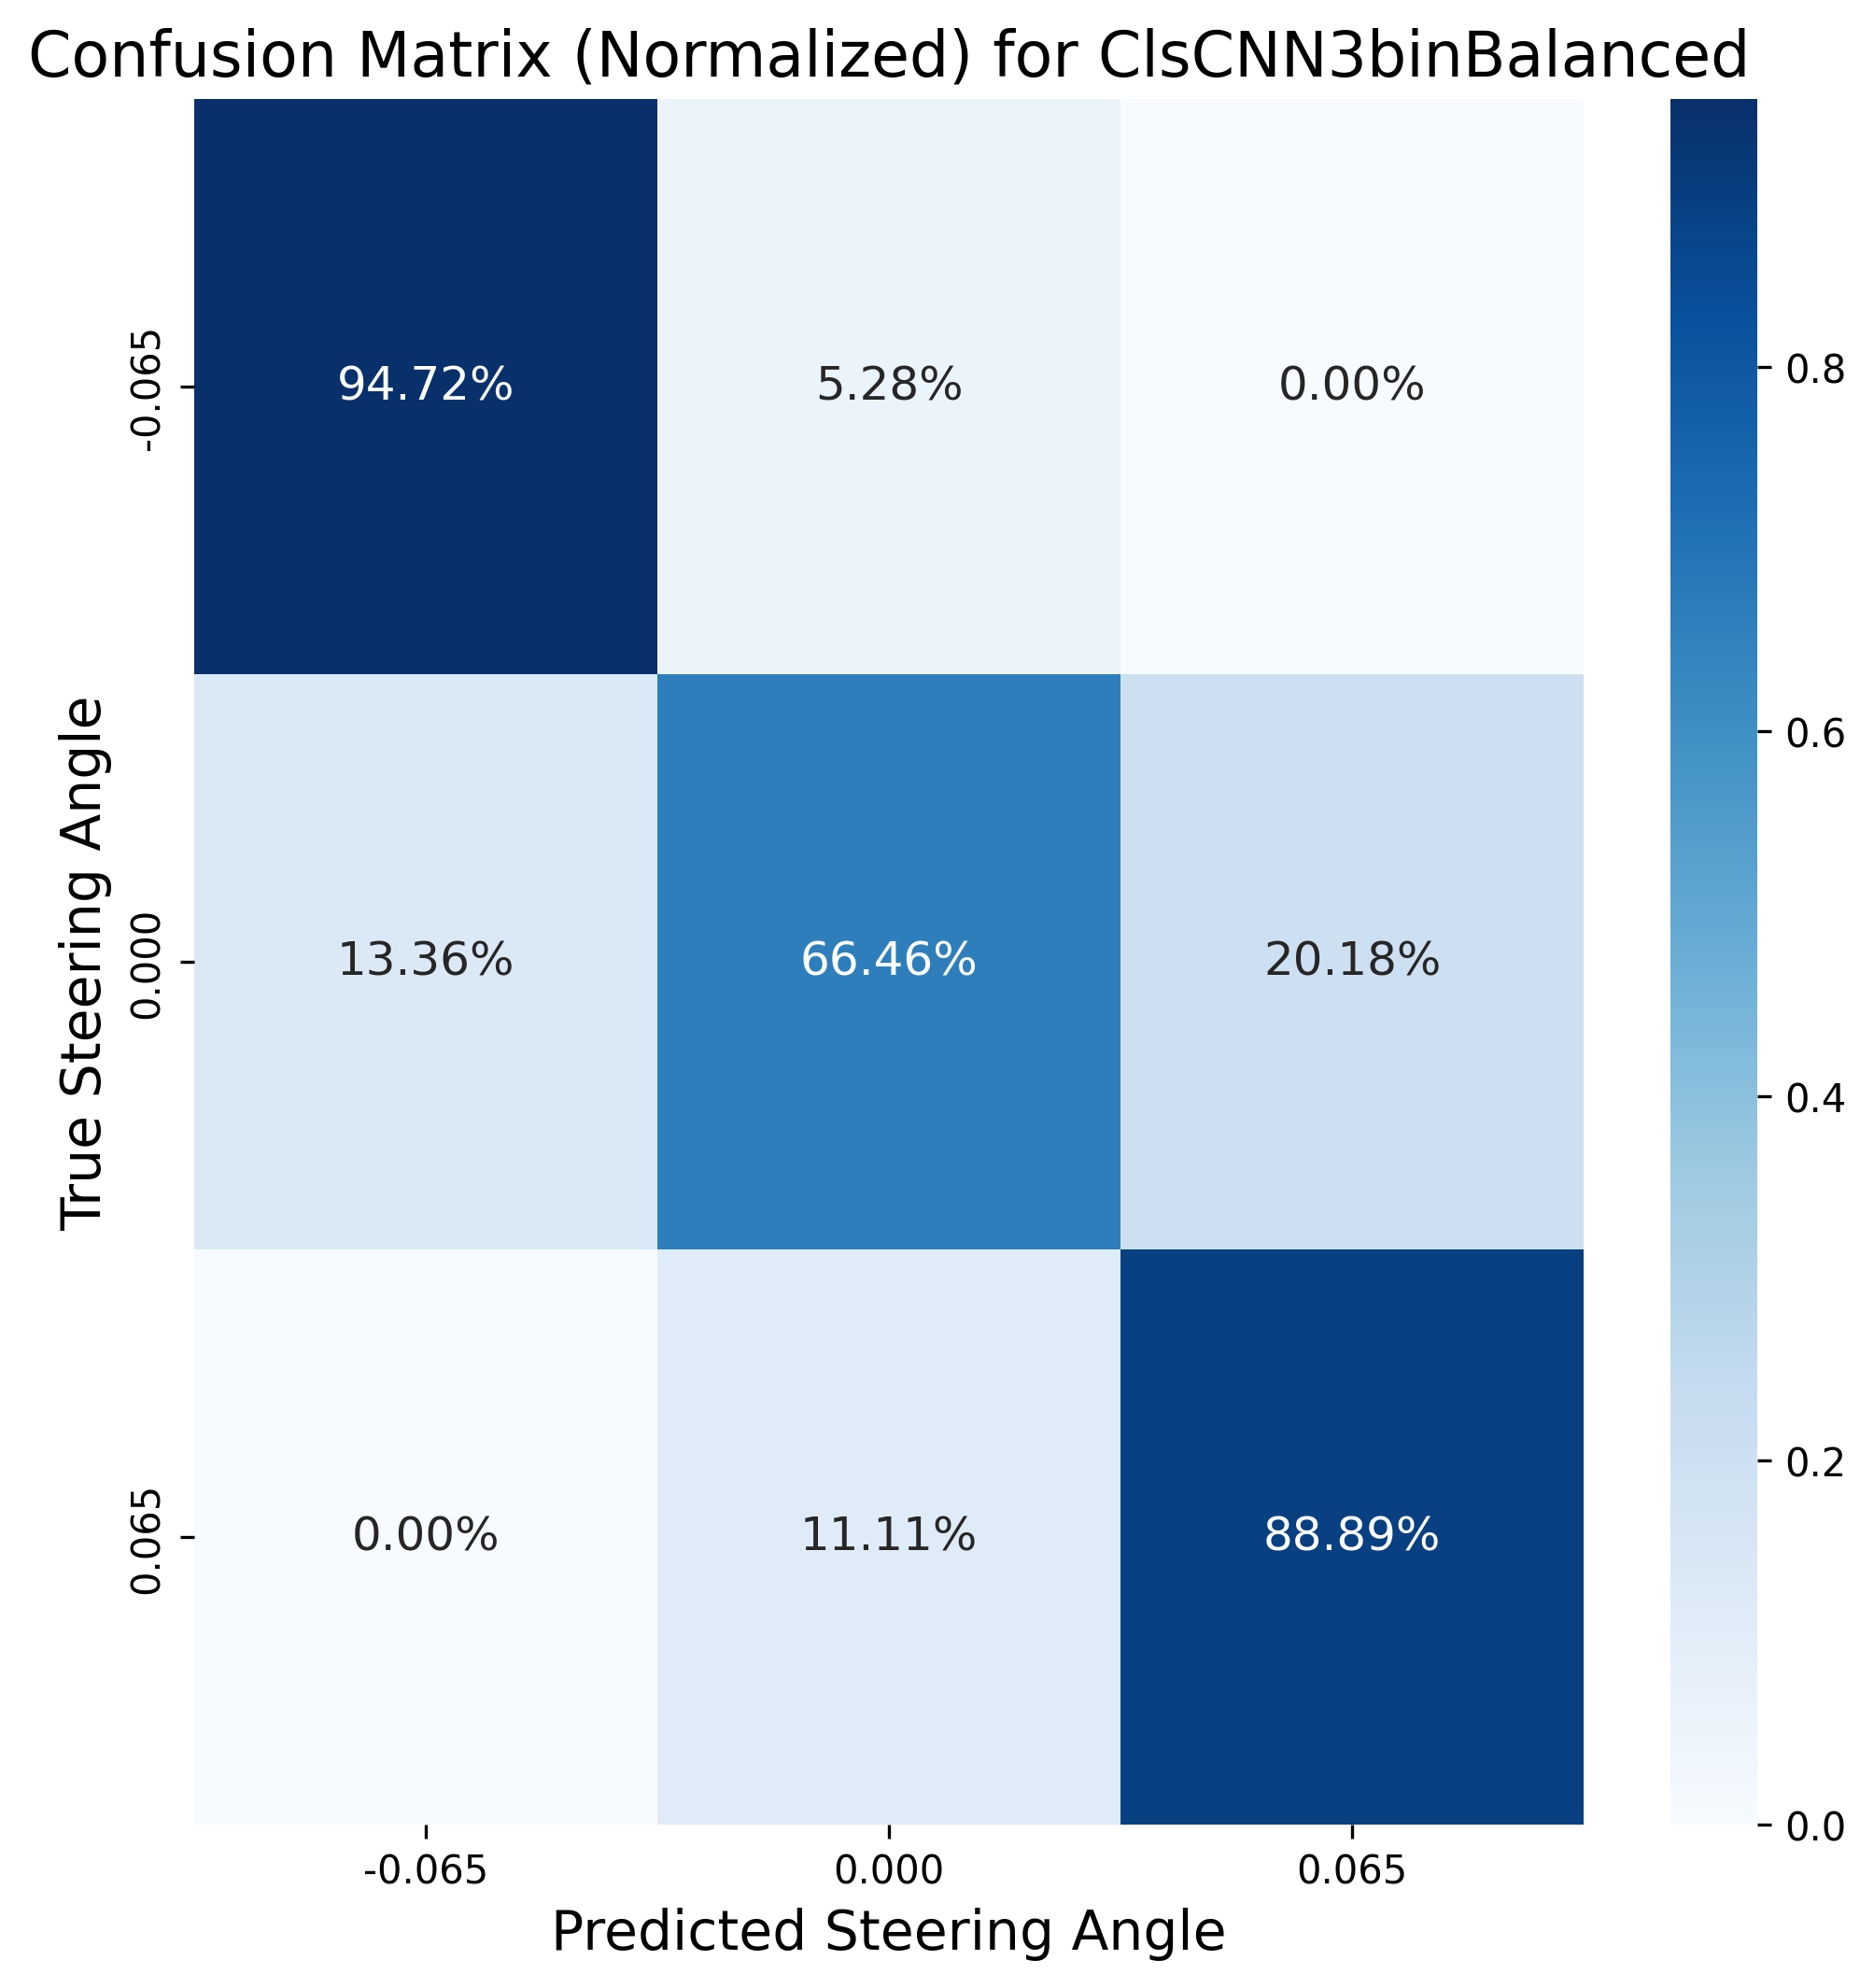
\includegraphics[width=0.65\linewidth]{Figures/Results/cm_norm_ClsCNN3binBalanced.png}
% \caption{ClsCNN3binBalanced model normalized confusion matrix}
% \label{fig:cm_norm_ClsCNN3binBalanced}
% \end{figure}

% %%%%%%%%%%%%%%%%%%%%%%%%
% % ClsCNN3binUnbalanced %
% %%%%%%%%%%%%%%%%%%%%%%%%

% \begin{table}[htbp]
% \centering
% \begin{tabular}{@{}lcccc@{}}
% \toprule
% \textbf{Class} & \textbf{Precision} & \textbf{Recall} & \textbf{F1-Score} & \textbf{Support} \\
% \midrule
% $-0.065$ & 0.61 & 0.28 & 0.38 & 1,422 \\
% $\phantom{-}0.000$ & 0.89 & 0.97 & 0.93 & 22,460 \\
% $\phantom{-}0.065$ & 0.79 & 0.42 & 0.55 & 3,059 \\
% \midrule
% \textbf{Macro Avg} & \textbf{0.76} & \textbf{0.56} & \textbf{0.62} & \textbf{26,941} \\
% \bottomrule
% \end{tabular}
% \caption{Classification performance results for the ClsCNN3binUnbalanced model. The model achieved an overall accuracy of 87.36\% with a mean confidence of 0.8682 across 26,941 test images.}
% \label{tab:clf_report_ClsCNN3binUnbalanced}
% \end{table}

% % ClsCNN3binUnbalanced Raw Counts Confusion Matrix %

% \begin{figure}[H]
% \centering
% 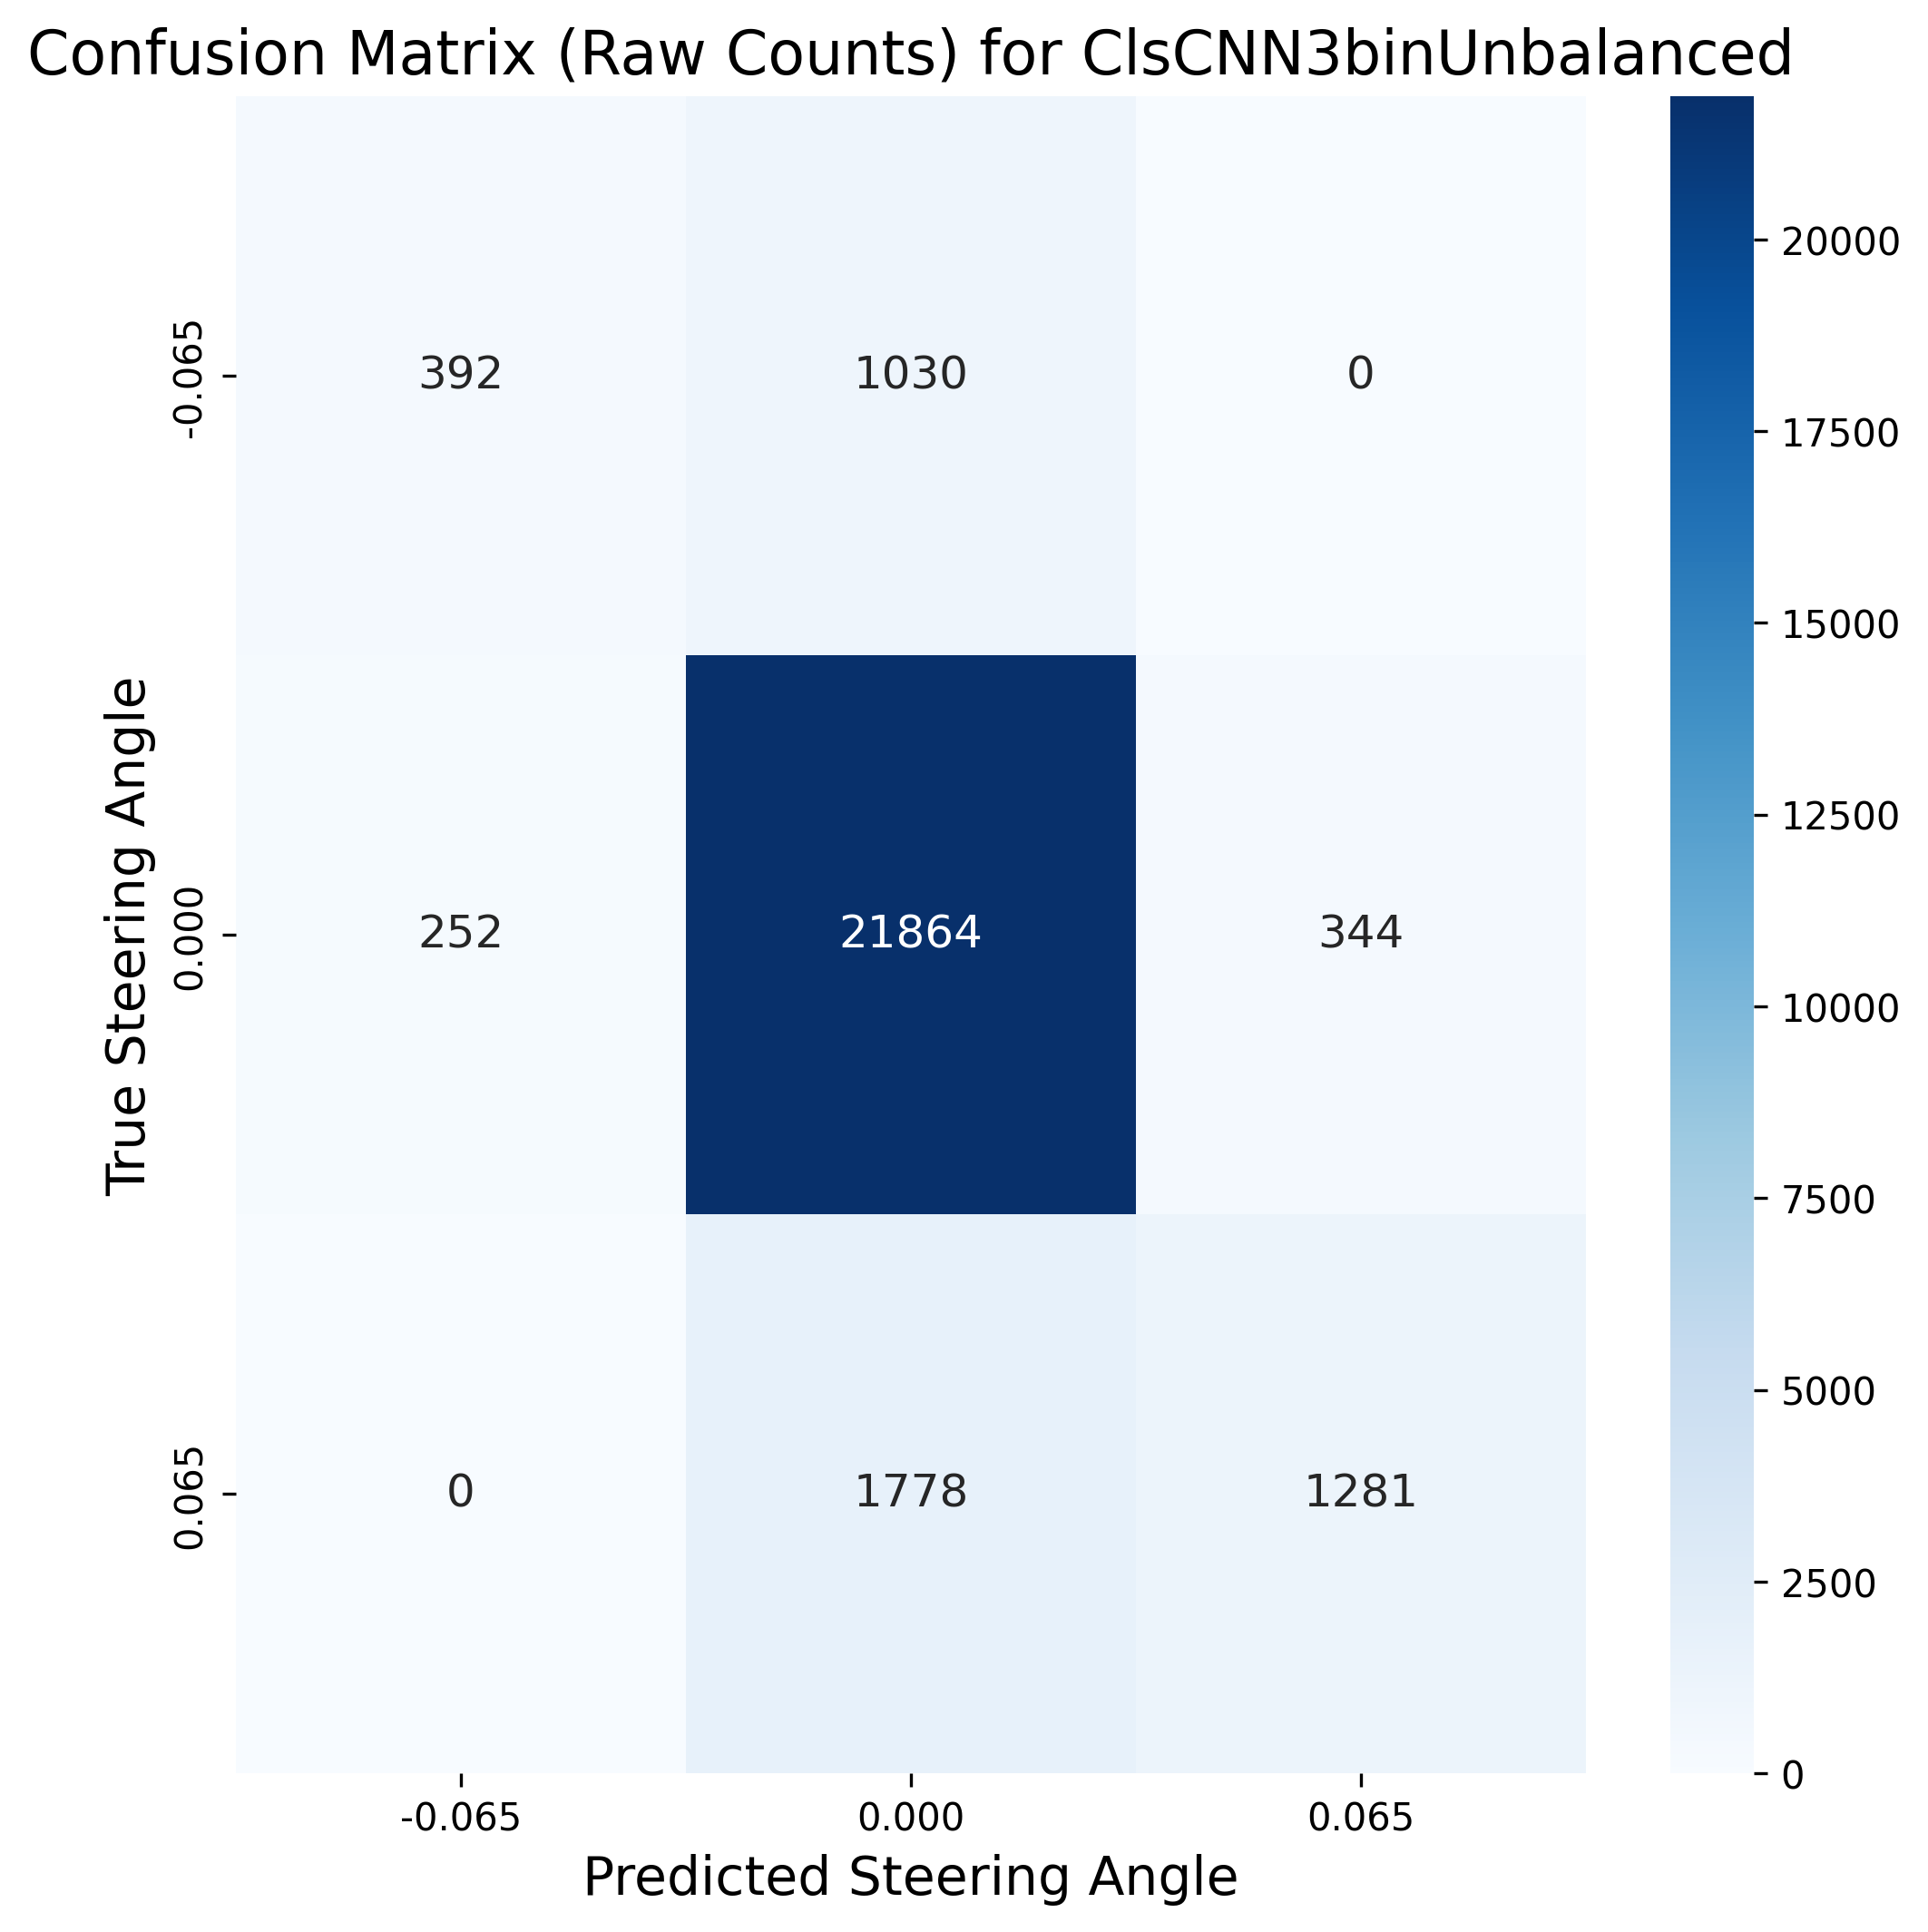
\includegraphics[width=0.65\linewidth]{Figures/Results/cm_raw_ClsCNN3binUnbalanced.png}
% \caption{ClsCNN3binUnbalanced model raw counts confusion matrix}
% \label{fig:cm_raw_ClsCNN3binUnbalanced}
% \end{figure}

% % ClsCNN3binUnbalanced Normalized Confusion Matrix %

% \begin{figure}[H]
% \centering
% 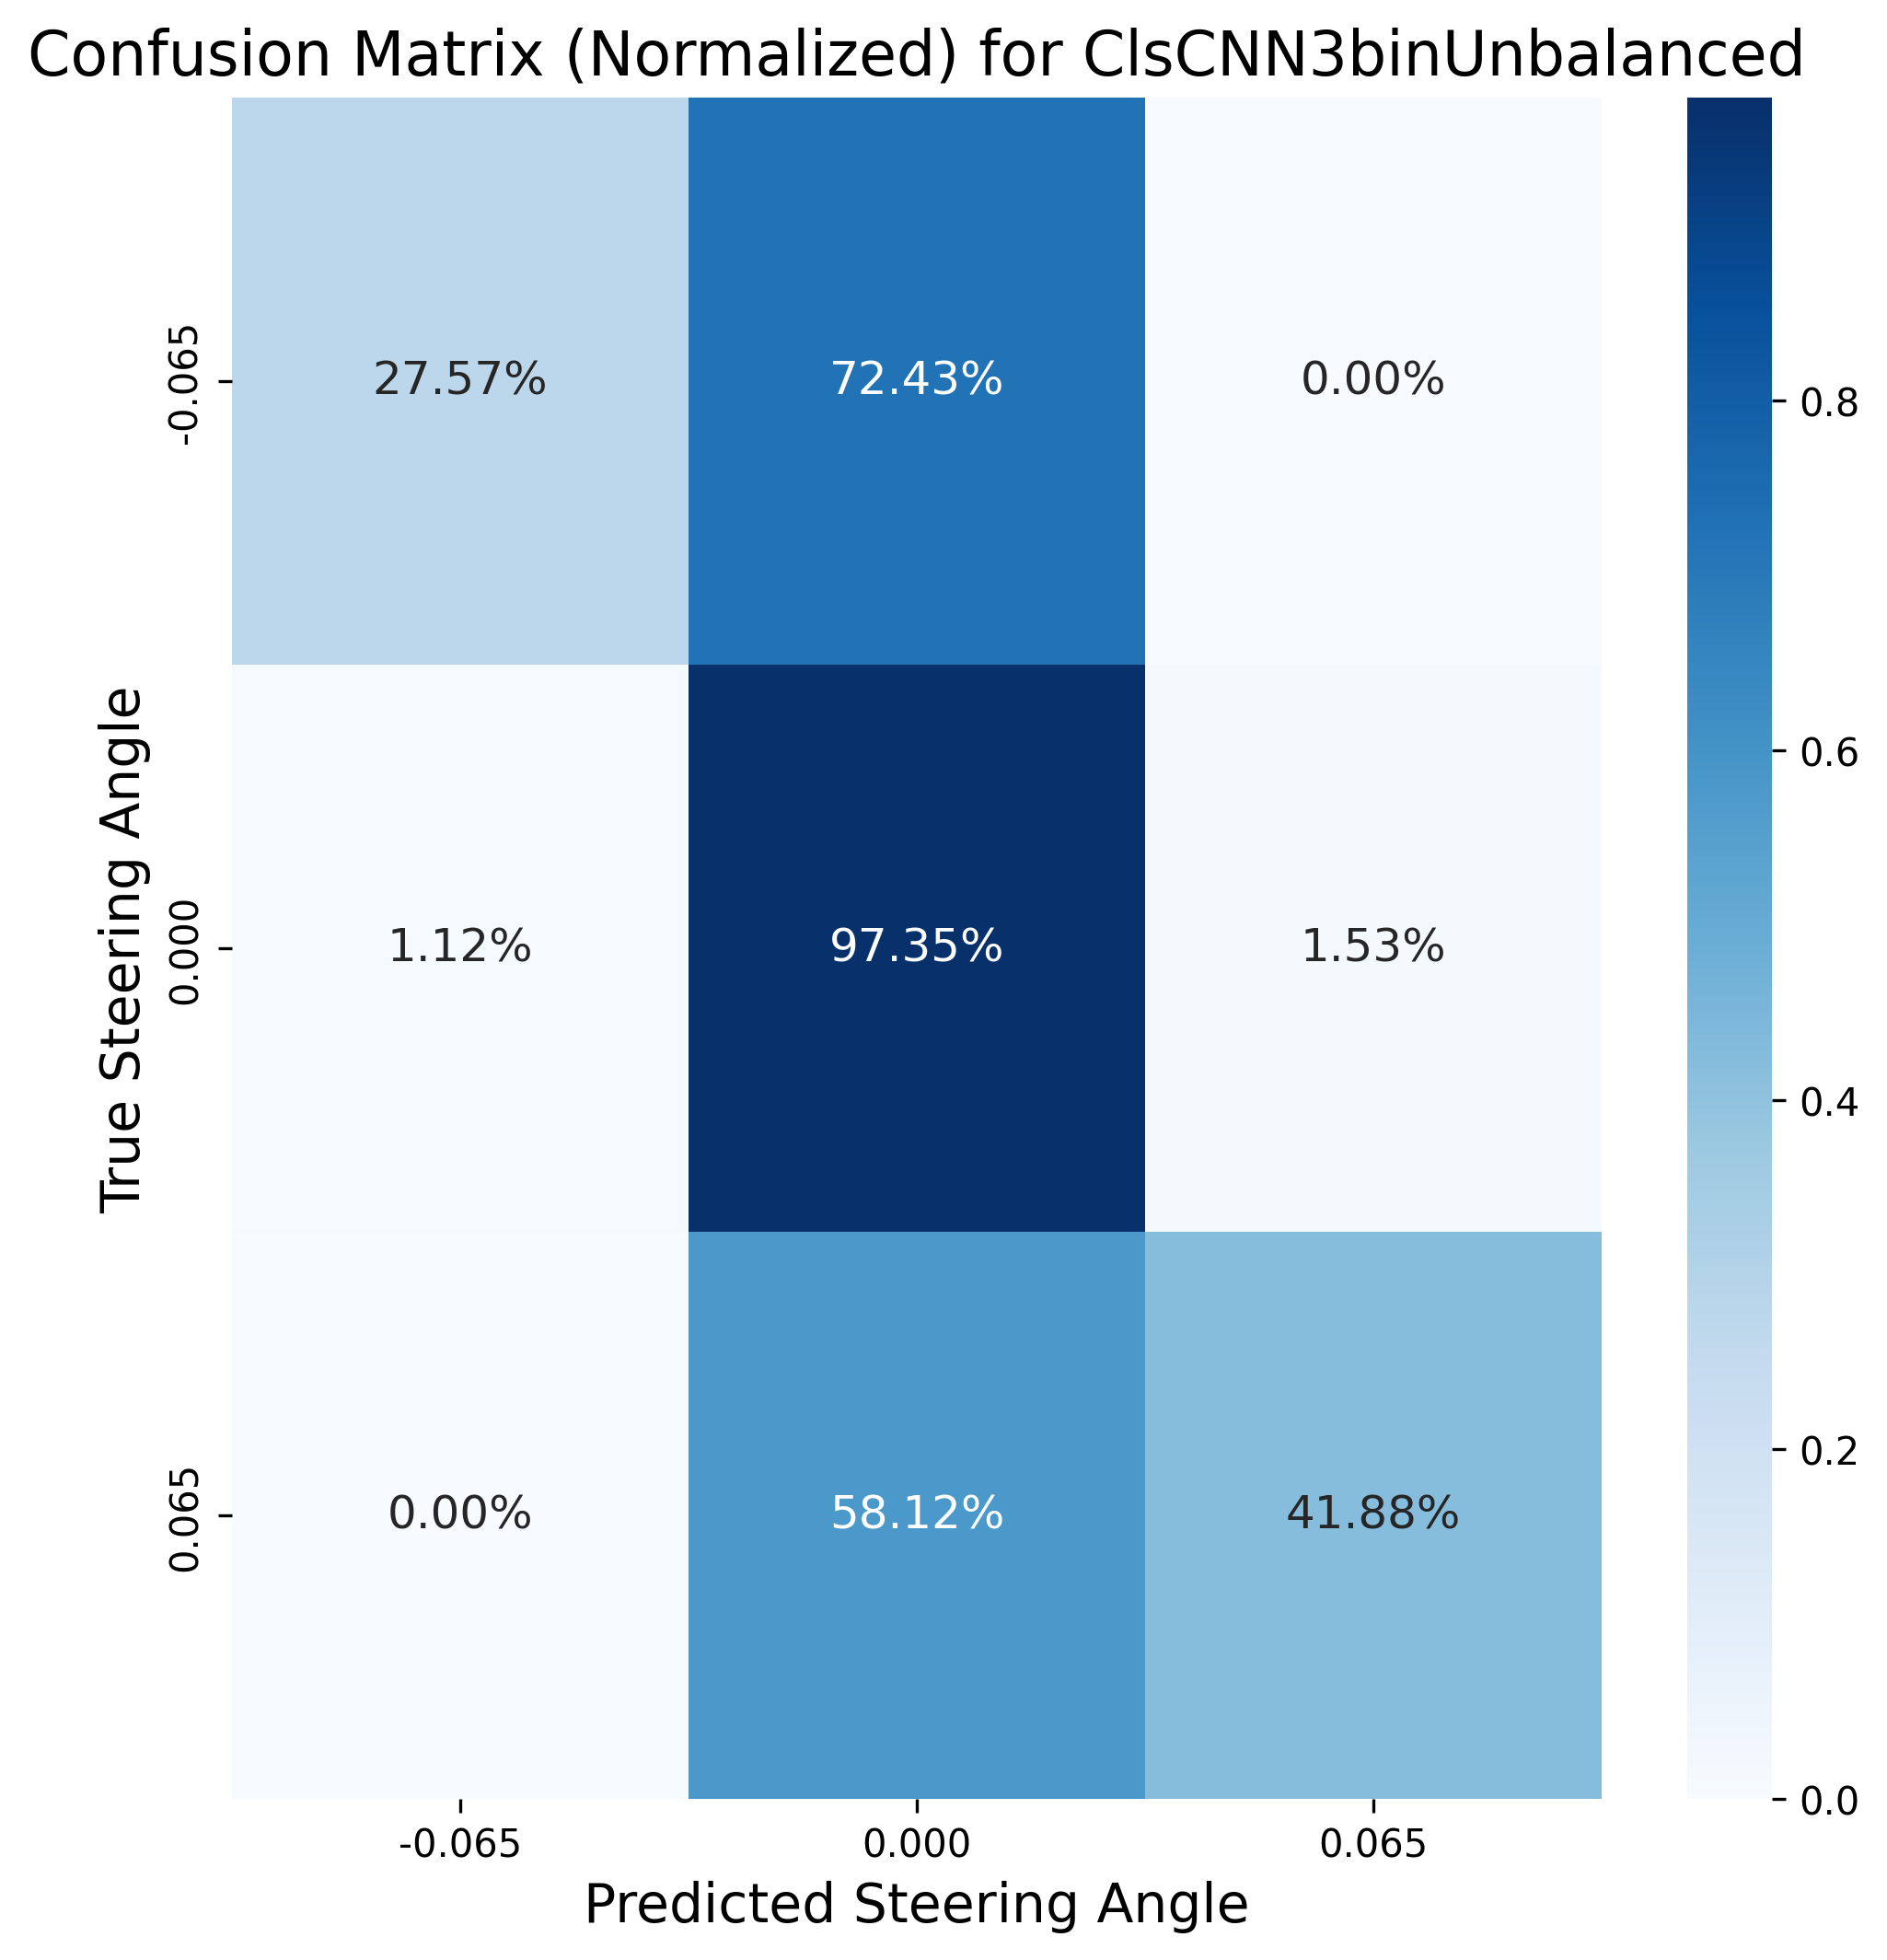
\includegraphics[width=0.65\linewidth]{Figures/Results/cm_norm_ClsCNN3binUnbalanced.png}
% \caption{ClsCNN3binUnbalanced model normalized confusion matrix}
% \label{fig:cm_norm_ClsCNN3binUnbalanced}
% \end{figure}

% %%%%%%%%%%%%%%%%%%%%%%
% % ClsCNN5binBalanced %
% %%%%%%%%%%%%%%%%%%%%%%

% \begin{table}[htbp]
% \centering
% \begin{tabular}{@{}lcccc@{}}
% \toprule
% \textbf{Class} & \textbf{Precision} & \textbf{Recall} & \textbf{F1-Score} & \textbf{Support} \\
% \midrule
% $-0.065$ & 0.89 & 0.99 & 0.94 & 15,839 \\
% $-0.015$ & 0.93 & 0.86 & 0.90 & 15,839 \\
% $\phantom{-}0.000$ & 0.96 & 0.94 & 0.95 & 15,839 \\
% $\phantom{-}0.015$ & 0.73 & 0.92 & 0.82 & 15,839 \\
% $\phantom{-}0.065$ & 0.92 & 0.67 & 0.77 & 15,839 \\
% \midrule
% \textbf{Macro Avg} & \textbf{0.89} & \textbf{0.88} & \textbf{0.88} & \textbf{79,195} \\
% \bottomrule
% \end{tabular}
% \caption{Classification performance results for the ClsCNN5binBalanced model. The model achieved an overall accuracy of 87.70\% with a mean confidence of 0.8762 across 79,195 test images.}
% \label{tab:clf_report_ClsCNN5binBalanced}
% \end{table}

% % ClsCNN5binBalanced Raw Counts Confusion Matrix %

% \begin{figure}[H]
% \centering
% 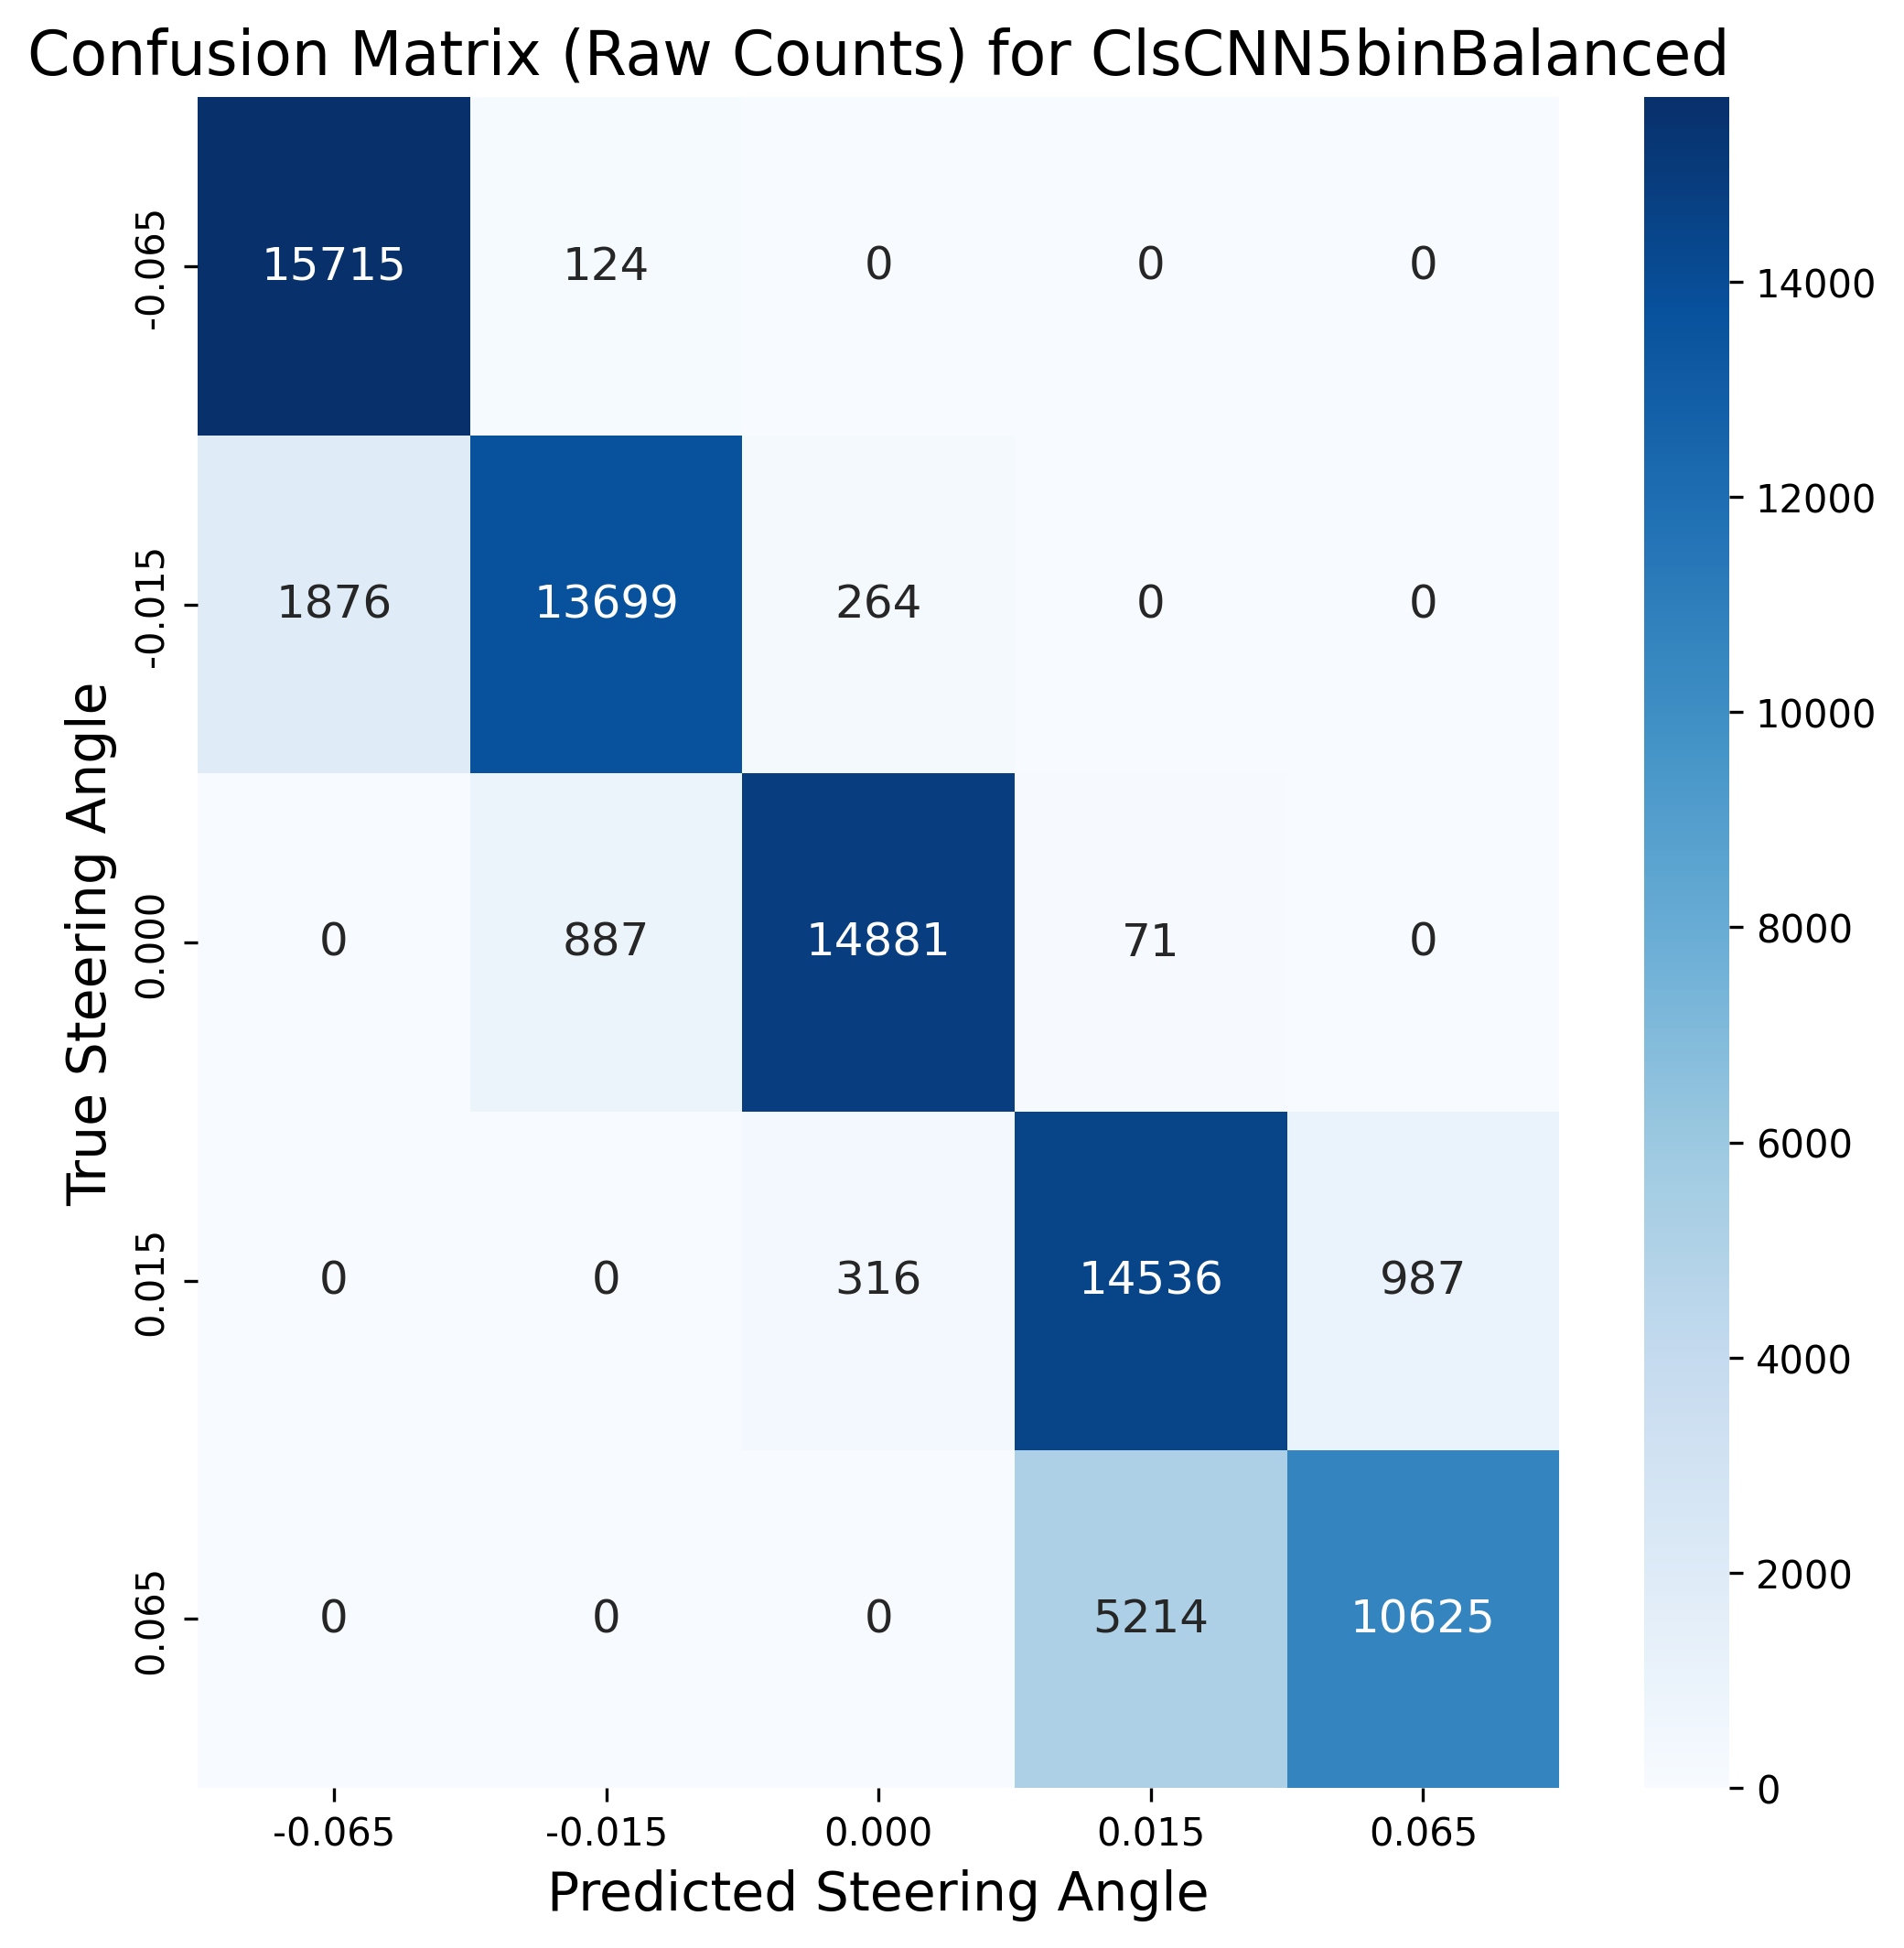
\includegraphics[width=0.65\linewidth]{Figures/Results/cm_raw_ClsCNN5binBalanced.png}
% \caption{ClsCNN5binBalanced model raw counts confusion matrix}
% \label{fig:cm_raw_ClsCNN5binBalanced}
% \end{figure}

% % ClsCNN5binBalanced Normalized Confusion Matrix %

% \begin{figure}[H]
% \centering
% 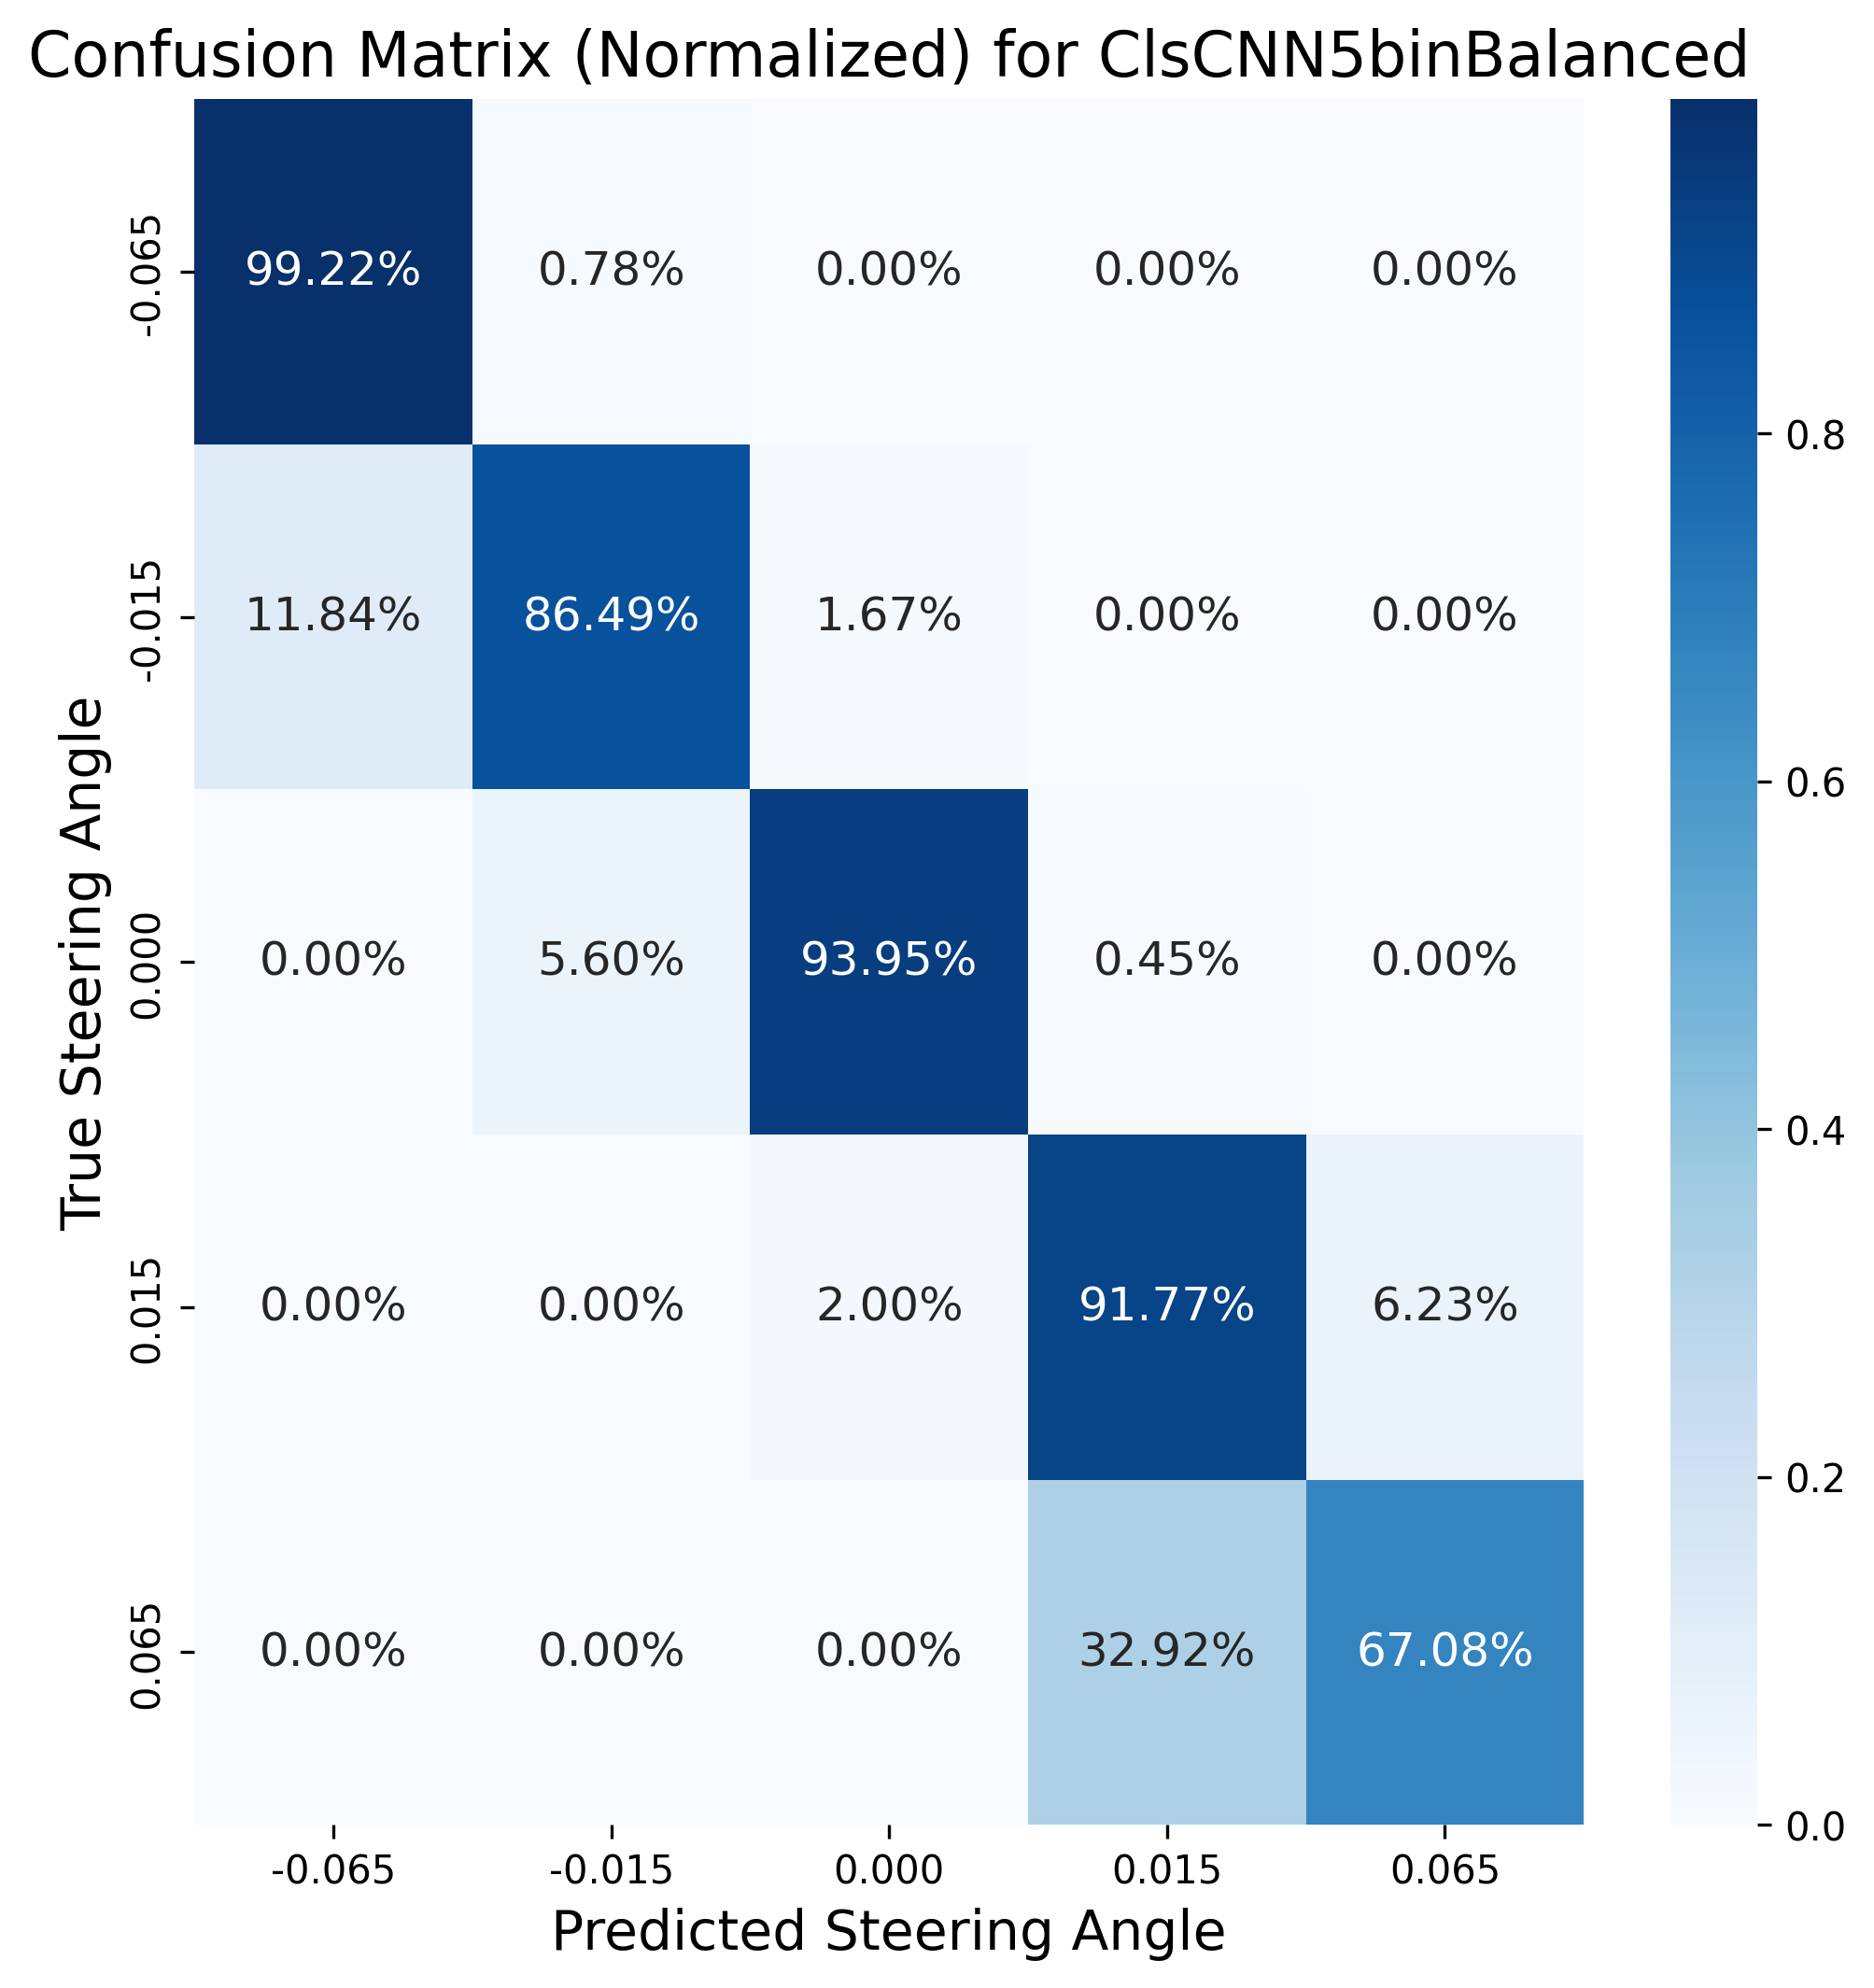
\includegraphics[width=0.65\linewidth]{Figures/Results/cm_norm_ClsCNN5binBalanced.png}
% \caption{ClsCNN5binBalanced model normalized confusion matrix}
% \label{fig:cm_norm_ClsCNN5binBalanced}
% \end{figure}

% %%%%%%%%%%%%%%%%%%%%%%%%
% % ClsCNN5binUnbalanced %
% %%%%%%%%%%%%%%%%%%%%%%%%

% \begin{table}[htbp]
% \centering
% \begin{tabular}{@{}lcccc@{}}
% \toprule
% \textbf{Class} & \textbf{Precision} & \textbf{Recall} & \textbf{F1-Score} & \textbf{Support} \\
% \midrule
% $-0.065$ & 0.80 & 0.36 & 0.50 & 401 \\
% $-0.015$ & 0.85 & 0.97 & 0.90 & 5,843 \\
% $\phantom{-}0.000$ & 0.98 & 0.95 & 0.97 & 15,839 \\
% $\phantom{-}0.015$ & 0.90 & 0.96 & 0.93 & 3,972 \\
% $\phantom{-}0.065$ & 0.87 & 0.57 & 0.69 & 936 \\
% \midrule
% \textbf{Macro Avg} & \textbf{0.88} & \textbf{0.76} & \textbf{0.80} & \textbf{26,991} \\
% \bottomrule
% \end{tabular}
% \caption{Classification performance results for the ClsCNN5binUnbalanced model. The model achieved an overall accuracy of 93.18\% with a mean confidence of 0.9294 across 26,991 test images.}
% \label{tab:clf_report_ClsCNN5binUnbalanced}
% \end{table}

% % ClsCNN5binUnbalanced Raw Counts Confusion Matrix %

% \begin{figure}[H]
% \centering
% 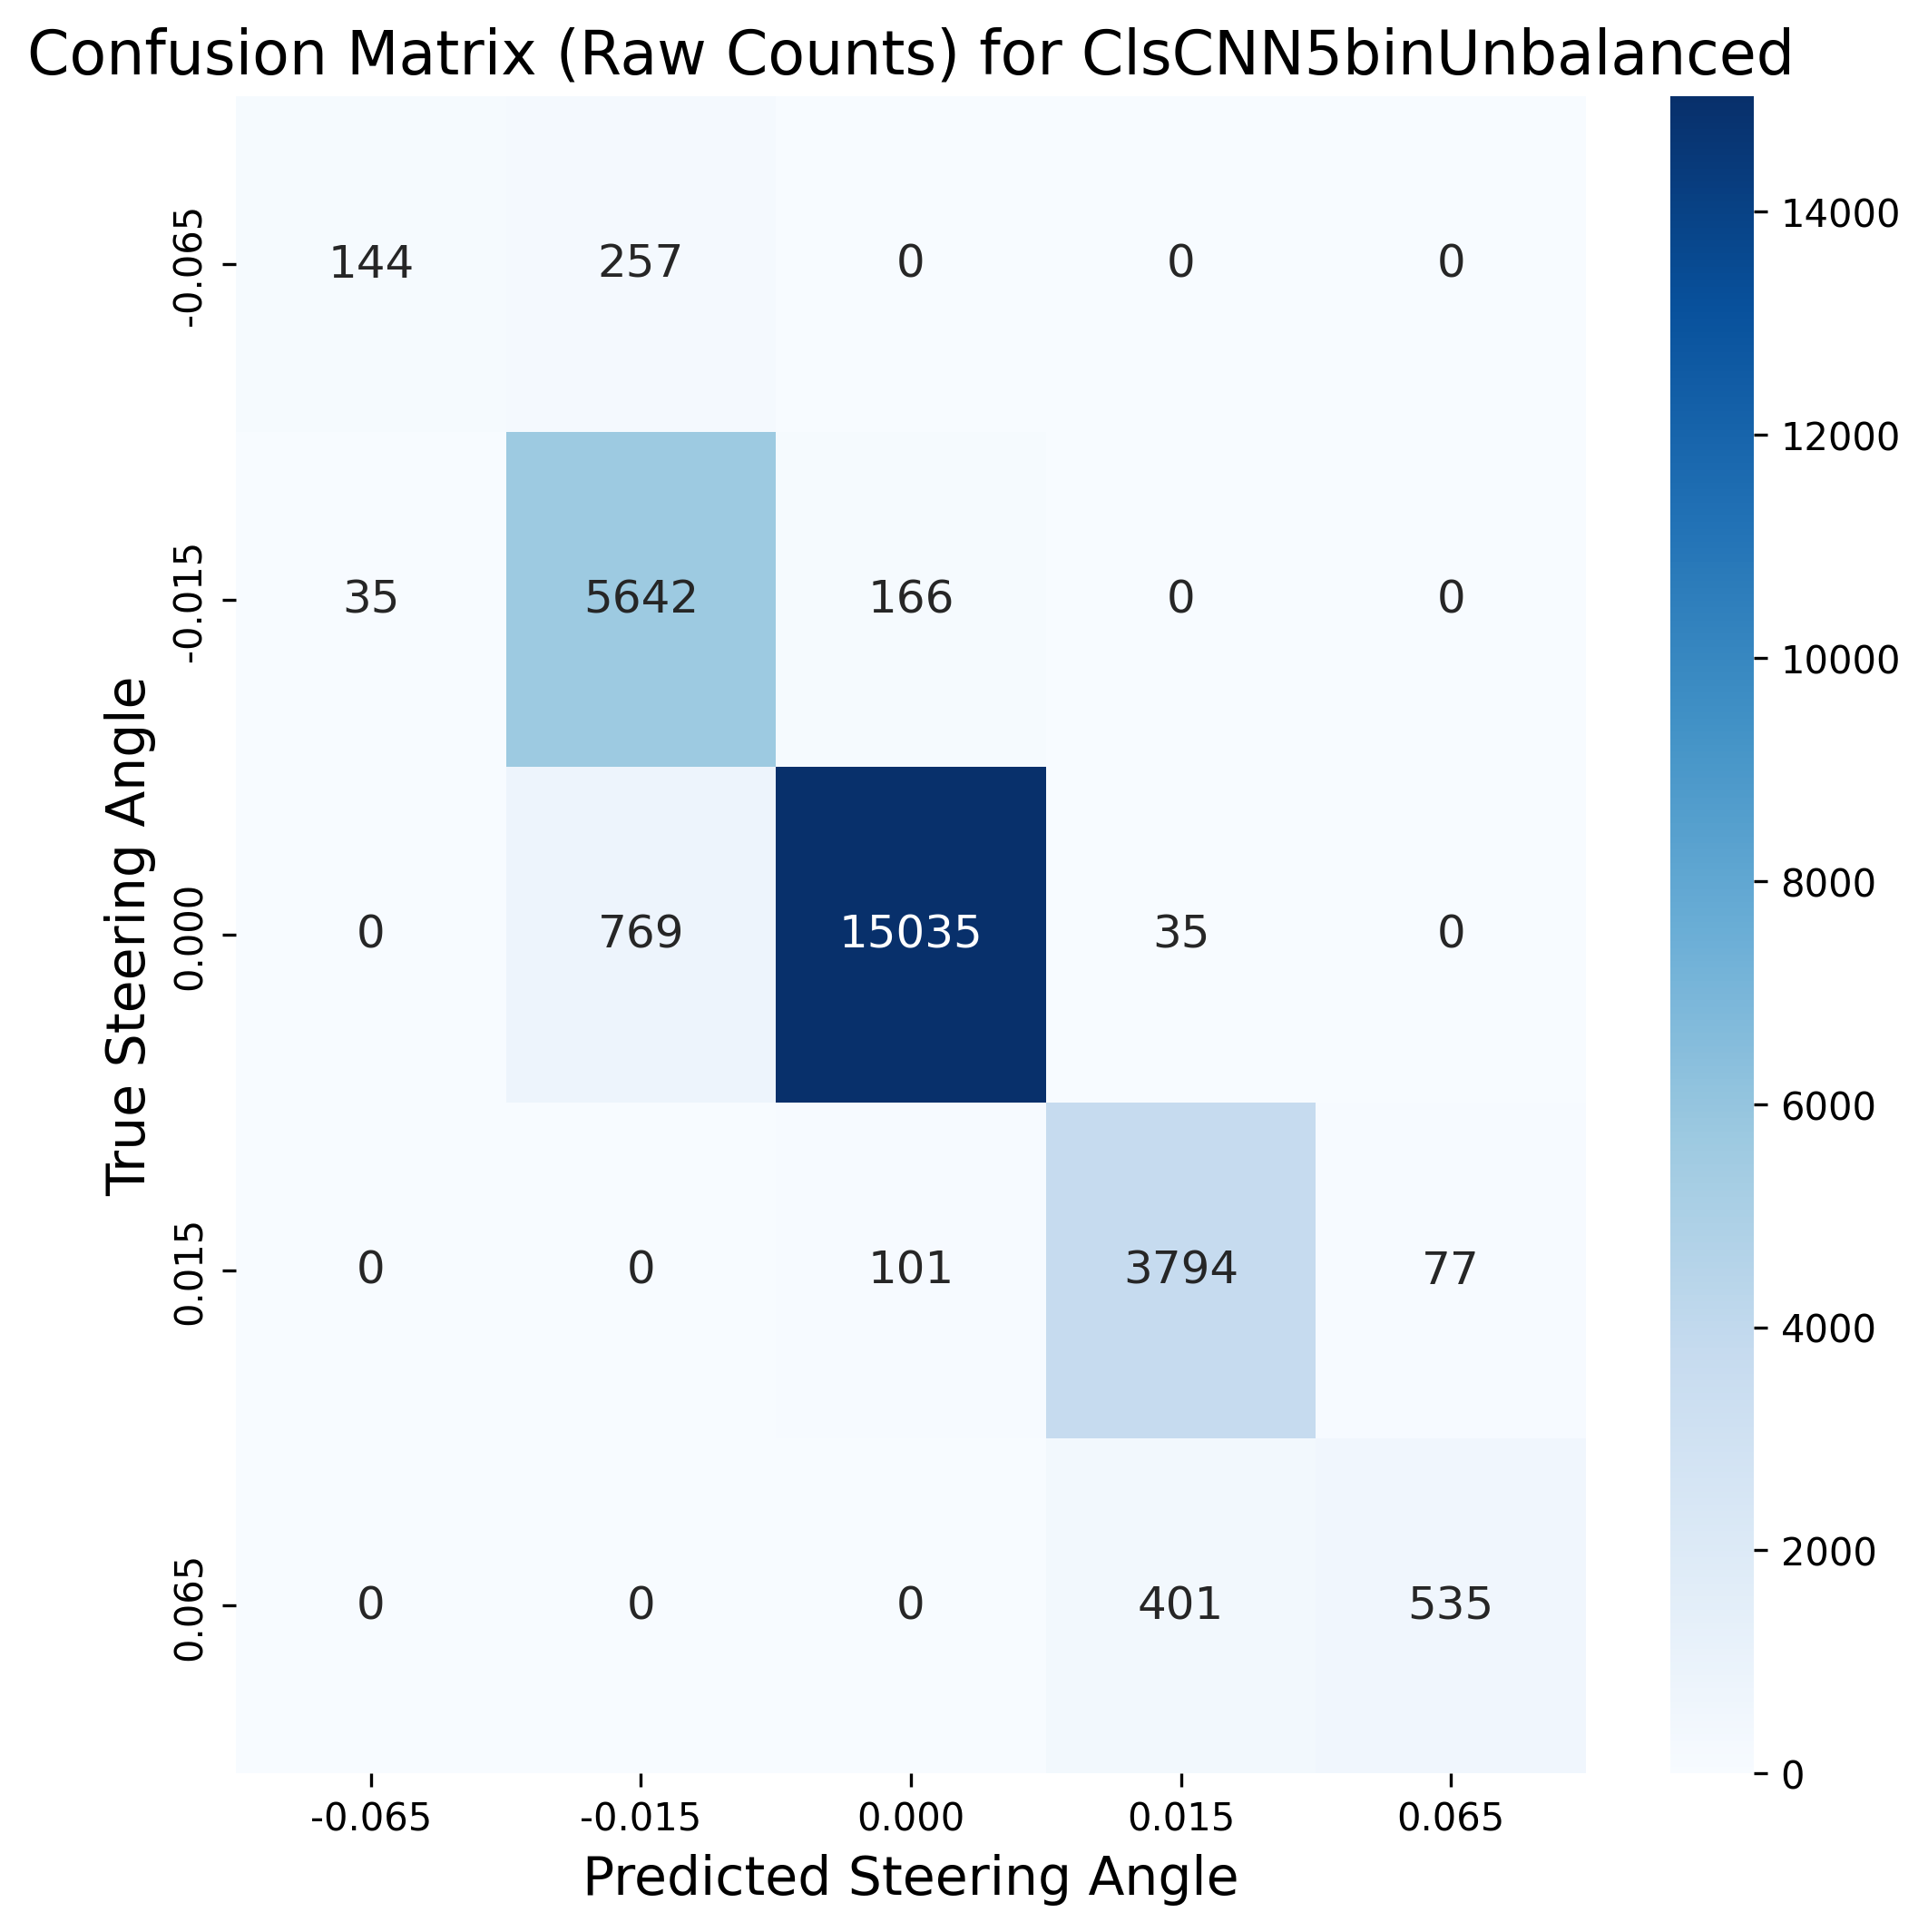
\includegraphics[width=0.65\linewidth]{Figures/Results/cm_raw_ClsCNN5binUnbalanced.png}
% \caption{ClsCNN5binUnbalanced model raw counts confusion matrix}
% \label{fig:cm_raw_ClsCNN5binUnbalanced}
% \end{figure}

% % ClsCNN5binUnbalanced Normalized Confusion Matrix %

% \begin{figure}[H]
% \centering
% 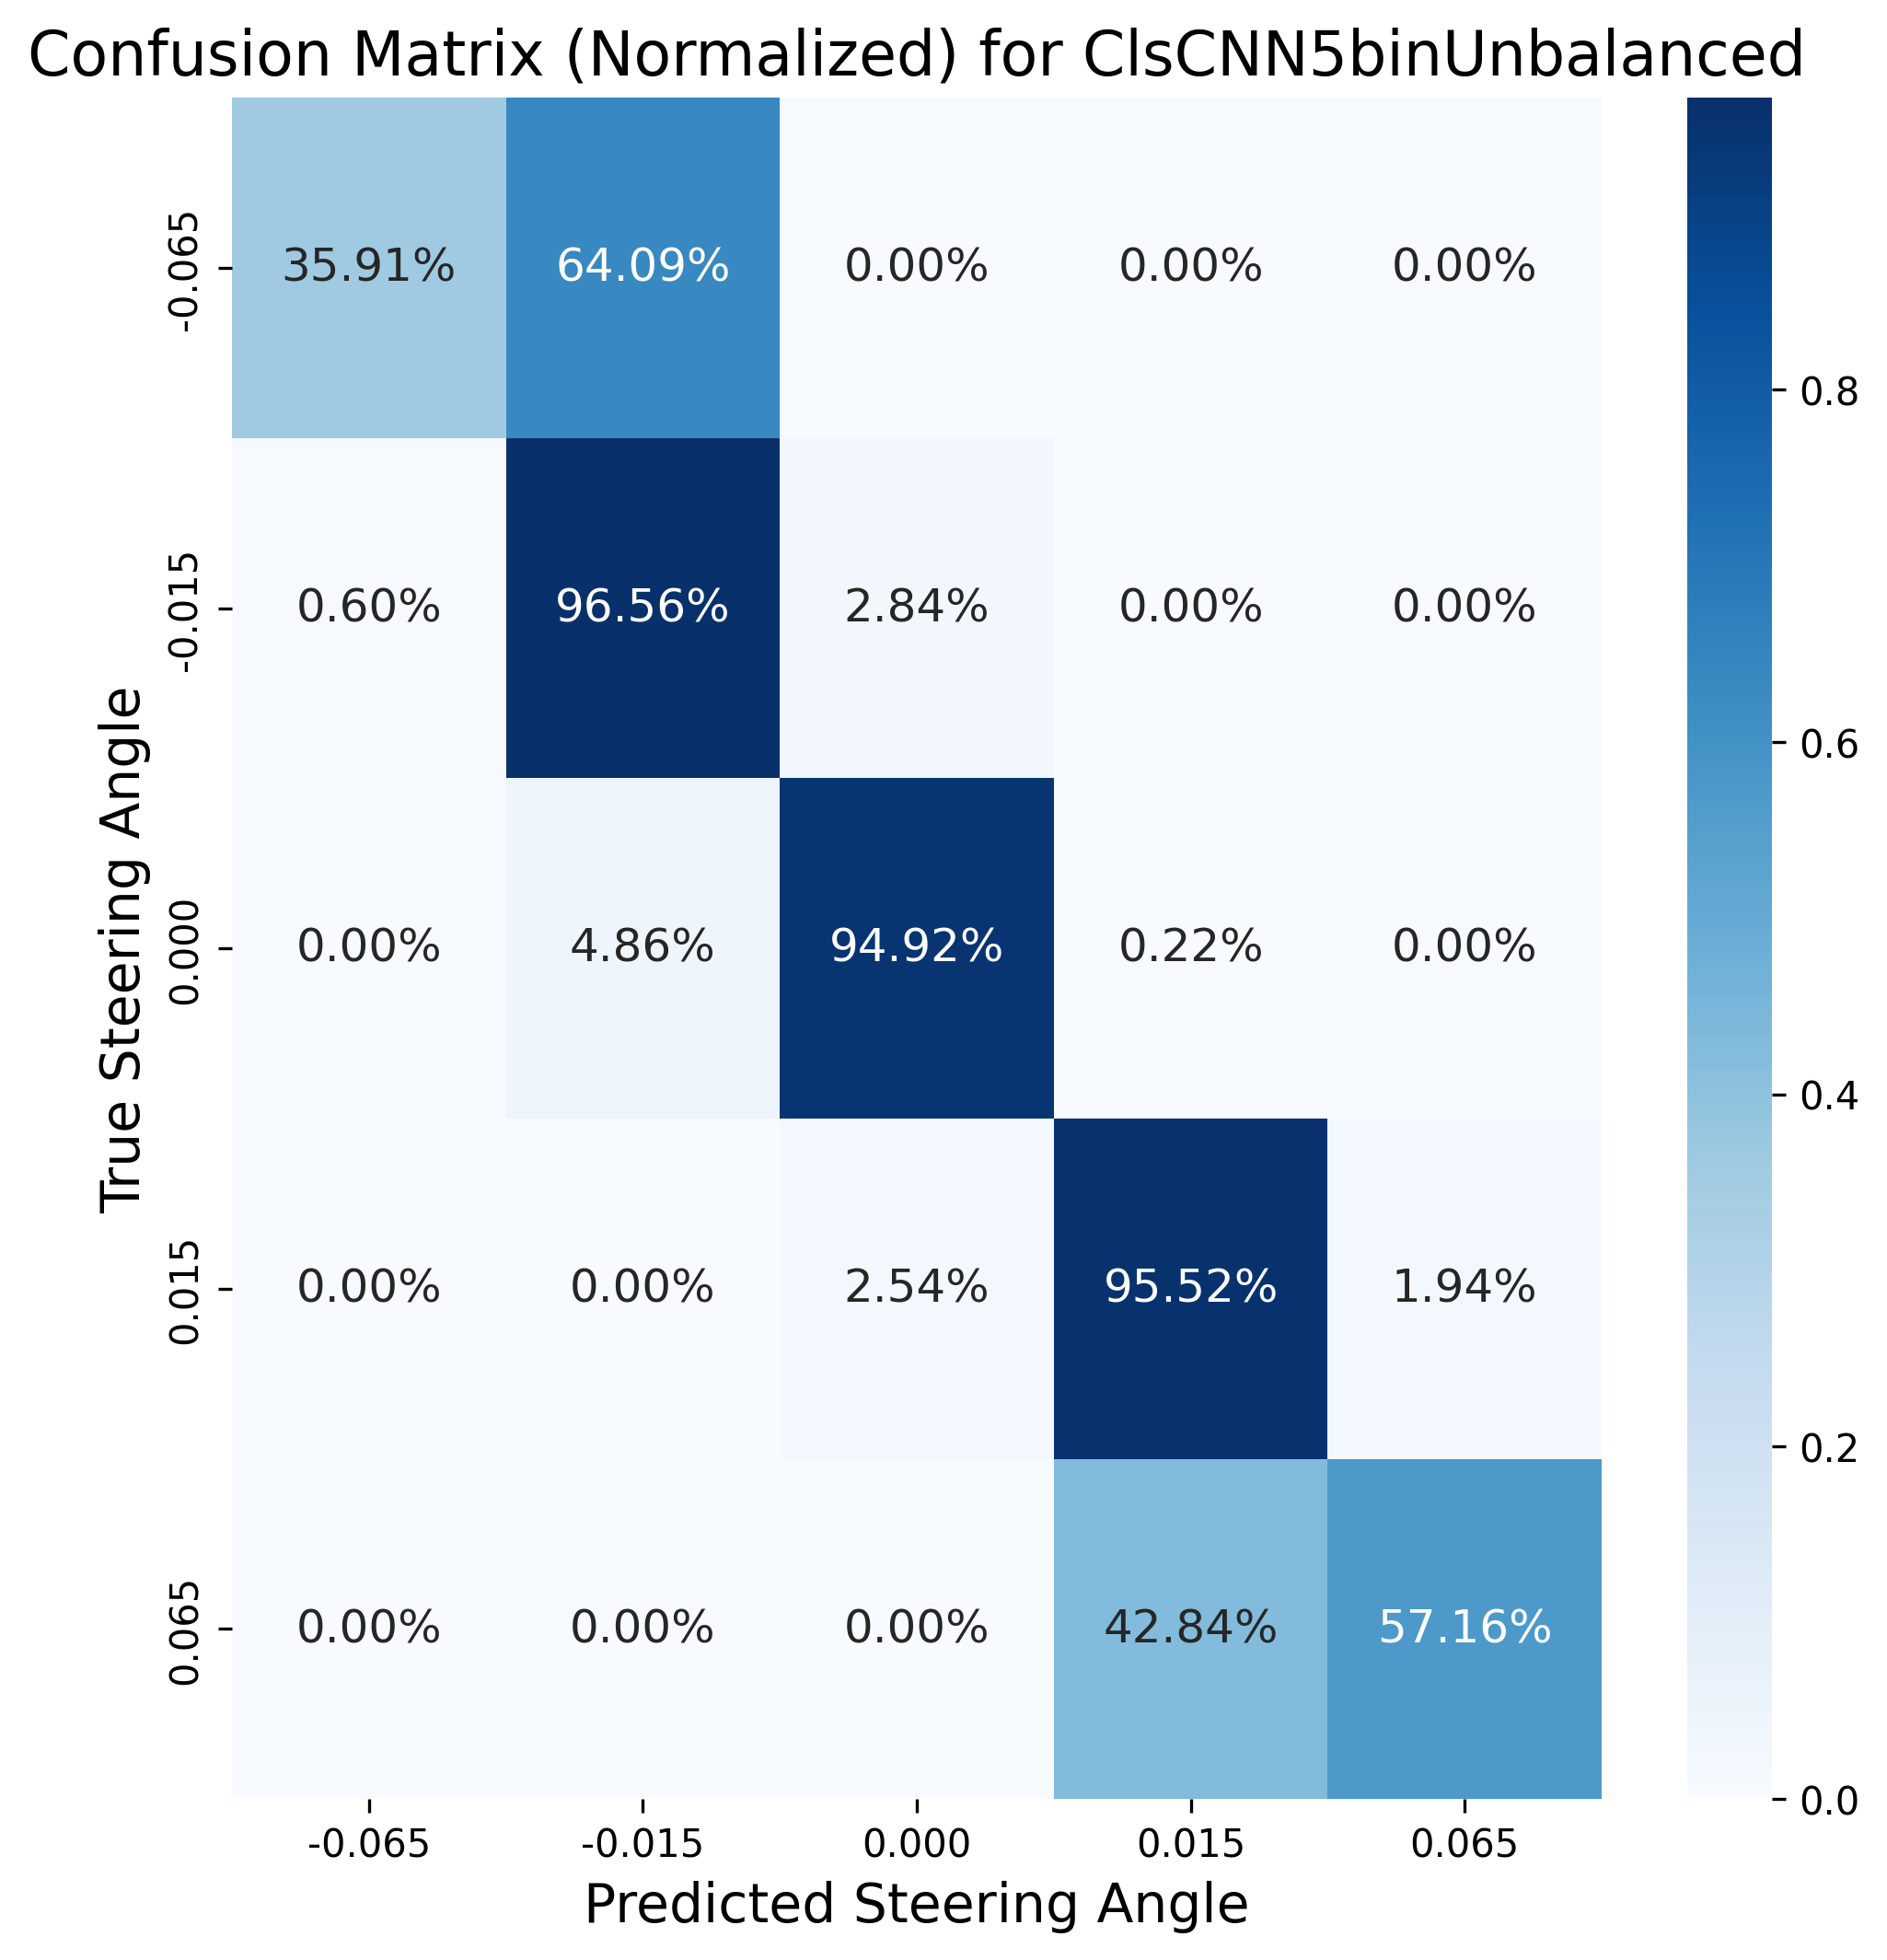
\includegraphics[width=0.65\linewidth]{Figures/Results/cm_norm_ClsCNN5binUnbalanced.png}
% \caption{ClsCNN5binUnbalanced model normalized confusion matrix}
% \label{fig:cm_norm_ClsCNN5binUnbalanced}
% \end{figure}

% %%%%%%%%%%%%%%%%%%%%%%%
% % ClsCNN15binBalanced %
% %%%%%%%%%%%%%%%%%%%%%%%

% \begin{table}[htbp]
% \centering
% \begin{tabular}{@{}lcccc@{}}
% \toprule
% \textbf{Class} & \textbf{Precision} & \textbf{Recall} & \textbf{F1-Score} & \textbf{Support} \\
% \midrule
% $-0.065$ & 0.37 & 0.43 & 0.40 & 10,199 \\
% $-0.055$ & 0.22 & 0.27 & 0.24 & 10,199 \\
% $-0.045$ & 0.34 & 0.39 & 0.36 & 10,199 \\
% $-0.035$ & 0.00 & 0.00 & 0.00 & 10,199 \\
% $-0.025$ & 0.40 & 0.60 & 0.48 & 10,199 \\
% $-0.015$ & 0.46 & 0.36 & 0.40 & 10,199 \\
% $-0.005$ & 0.77 & 0.95 & 0.85 & 10,199 \\
% $\phantom{-}0.000$ & 0.85 & 0.94 & 0.89 & 10,199 \\
% $\phantom{-}0.005$ & 0.54 & 0.81 & 0.65 & 10,199 \\
% $\phantom{-}0.015$ & 0.51 & 0.12 & 0.20 & 10,199 \\
% $\phantom{-}0.025$ & 0.46 & 0.40 & 0.43 & 10,199 \\
% $\phantom{-}0.035$ & 0.44 & 0.54 & 0.48 & 10,199 \\
% $\phantom{-}0.045$ & 0.48 & 0.31 & 0.38 & 10,199 \\
% $\phantom{-}0.055$ & 0.38 & 0.77 & 0.51 & 10,199 \\
% $\phantom{-}0.065$ & 0.85 & 0.31 & 0.45 & 10,199 \\
% \midrule
% \textbf{Macro Avg} & \textbf{0.47} & \textbf{0.48} & \textbf{0.45} & \textbf{152,985} \\
% \bottomrule
% \end{tabular}
% \caption{Classification performance results for the ClsCNN15binBalanced model. The model achieved an overall accuracy of 48.01\% with a mean confidence of 0.4809 across 152,985 test images.}
% \label{tab:clf_report_ClsCNN15binBalanced}
% \end{table}

% % ClsCNN15binBalanced Raw Counts Confusion Matrix %

% \begin{figure}[H]
% \centering
% 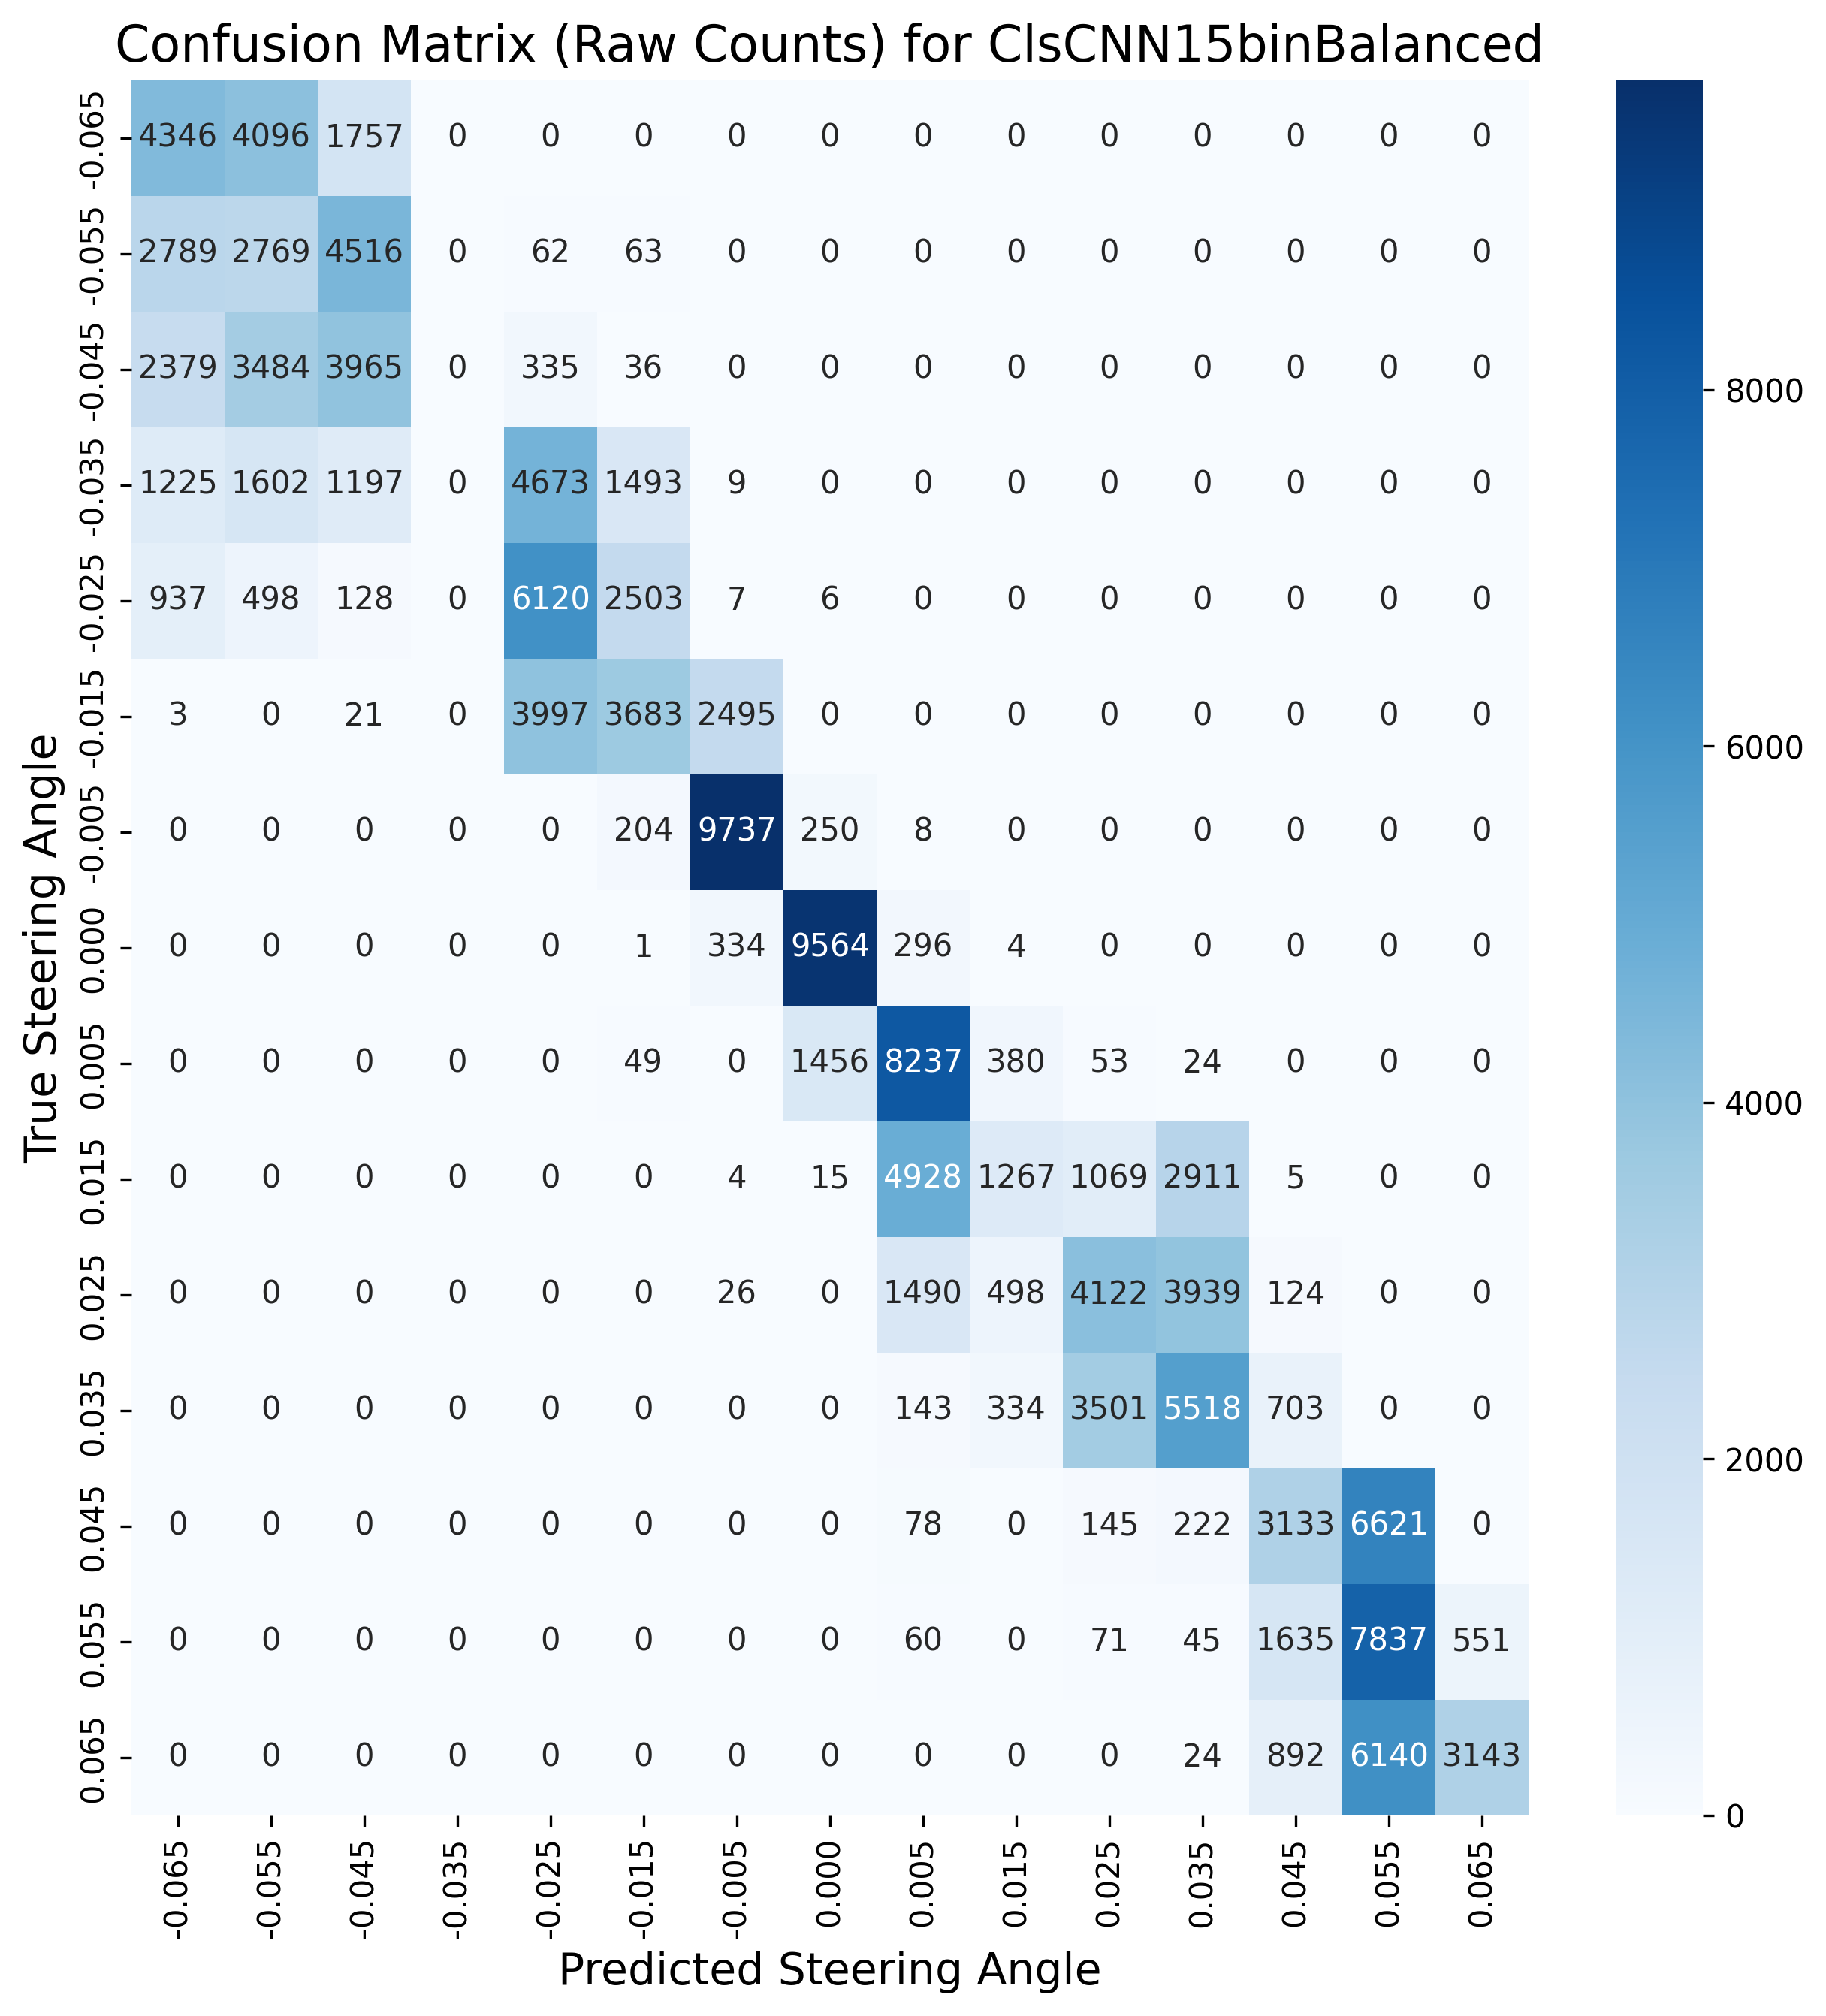
\includegraphics[width=1\linewidth]{Figures/Results/cm_raw_ClsCNN15binBalanced.png}
% \caption{ClsCNN15binBalanced model raw counts confusion matrix}
% \label{fig:cm_raw_ClsCNN15binBalanced}
% \end{figure}

% % ClsCNN15binBalanced Normalized Confusion Matrix %

% \begin{figure}[H]
% \centering
% 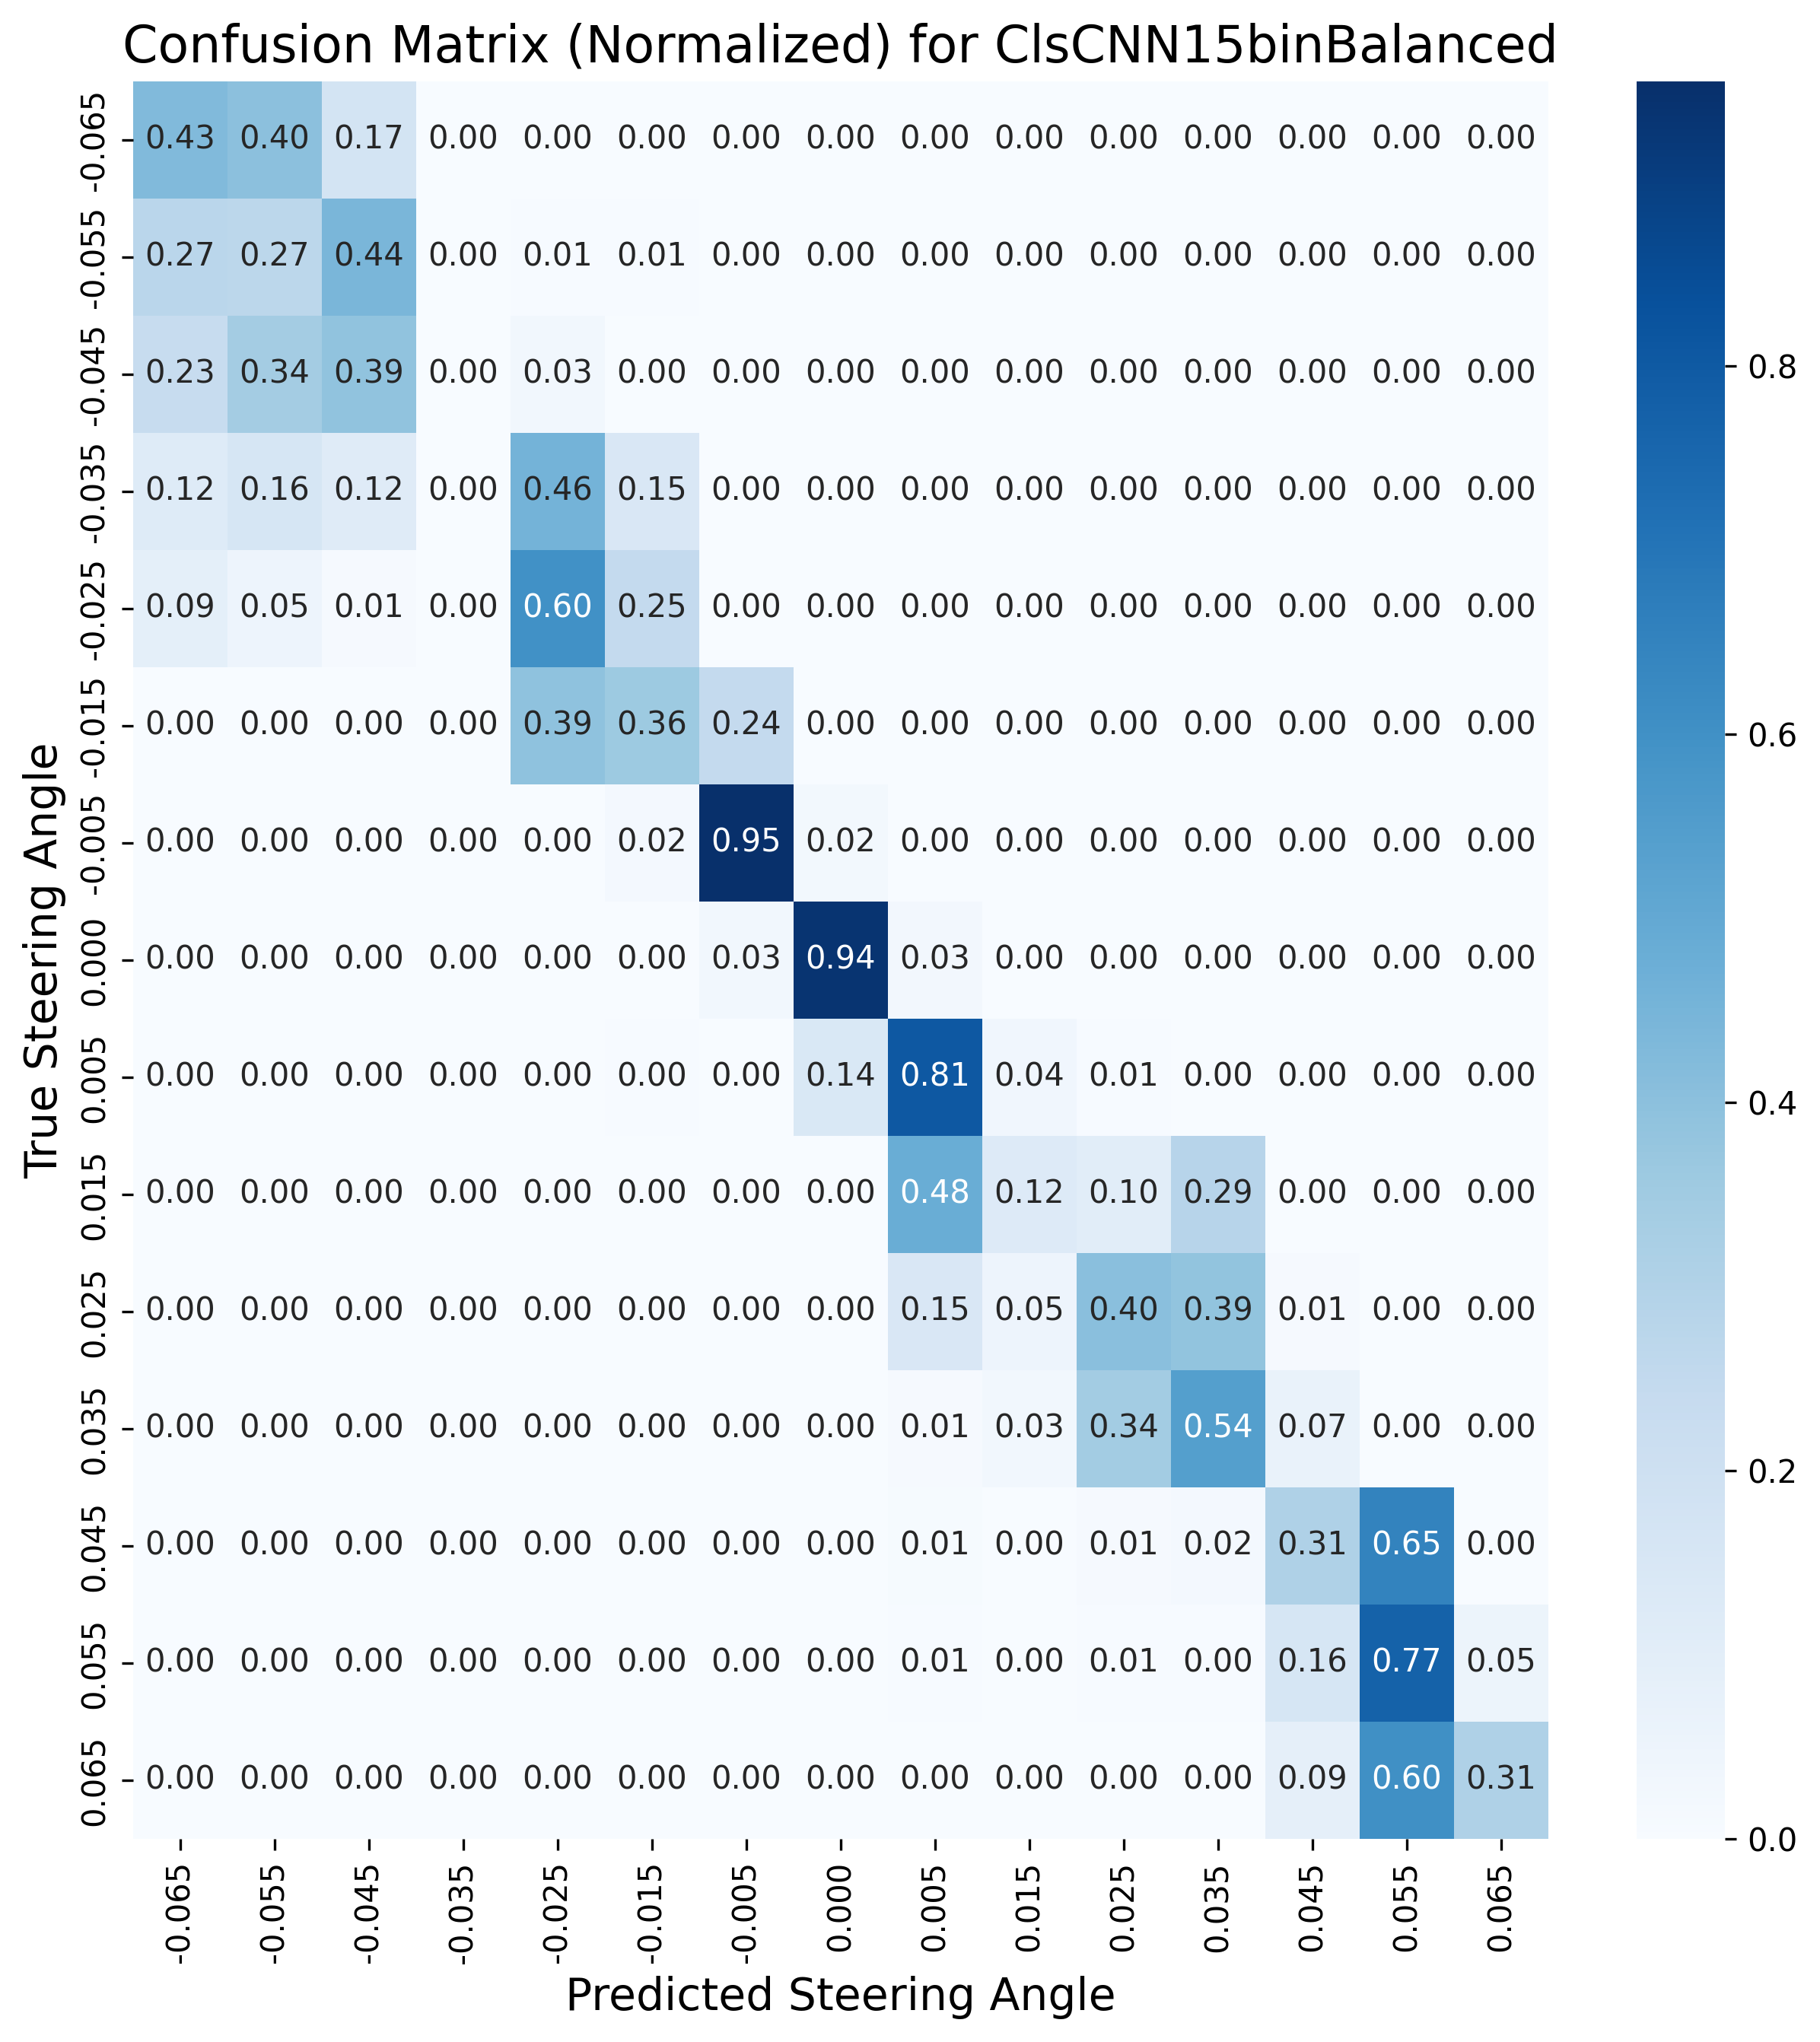
\includegraphics[width=1\linewidth]{Figures/Results/cm_norm_ClsCNN15binBalanced.png}
% \caption{ClsCNN15binBalanced model normalized confusion matrix}
% \label{fig:cm_norm_ClsCNN15binBalanced}
% \end{figure}

% %%%%%%%%%%%%%%%%%%%%%%%%%
% % ClsCNN15binUnbalanced %
% %%%%%%%%%%%%%%%%%%%%%%%%%

% \begin{table}[htbp]
% \centering
% \begin{tabular}{@{}lcccc@{}}
% \toprule
% \textbf{Class} & \textbf{Precision} & \textbf{Recall} & \textbf{F1-Score} & \textbf{Support} \\
% \midrule
% $-0.065$ & 0.00 & 0.00 & 0.00 & 128 \\
% $-0.055$ & 0.00 & 0.00 & 0.00 & 141 \\
% $-0.045$ & 0.00 & 0.00 & 0.00 & 223 \\
% $-0.035$ & 0.35 & 0.37 & 0.36 & 1,027 \\
% $-0.025$ & 0.49 & 0.04 & 0.07 & 2,094 \\
% $-0.015$ & 0.60 & 0.74 & 0.66 & 4,986 \\
% $-0.005$ & 0.87 & 0.96 & 0.91 & 10,199 \\
% $\phantom{-}0.000$ & 0.91 & 0.96 & 0.93 & 4,896 \\
% $\phantom{-}0.005$ & 0.00 & 0.00 & 0.00 & 883 \\
% $\phantom{-}0.015$ & 0.63 & 0.91 & 0.75 & 2,665 \\
% $\phantom{-}0.025$ & 0.47 & 0.32 & 0.38 & 827 \\
% $\phantom{-}0.035$ & 0.00 & 0.00 & 0.00 & 240 \\
% $\phantom{-}0.045$ & 0.00 & 0.00 & 0.00 & 124 \\
% $\phantom{-}0.055$ & 0.00 & 0.00 & 0.00 & 150 \\
% $\phantom{-}0.065$ & 0.58 & 0.99 & 0.73 & 408 \\
% \midrule
% \textbf{Macro Avg} & \textbf{0.33} & \textbf{0.35} & \textbf{0.32} & \textbf{28,991} \\
% \bottomrule
% \end{tabular}
% \caption{Classification performance results for the ClsCNN15binUnbalanced model. The model achieved an overall accuracy of 75.11\% with a mean confidence of 0.7495 across 28,991 test images.}
% \label{tab:clf_report_ClsCNN15binUnbalanced}
% \end{table}

% %% GENERATED BY SCRIPT 18-generate-oacc-cnn-classifiers.py
% % ClsCNN15binUnbalanced Raw Counts Confusion Matrix %

% \begin{figure}[H]
% \centering
% 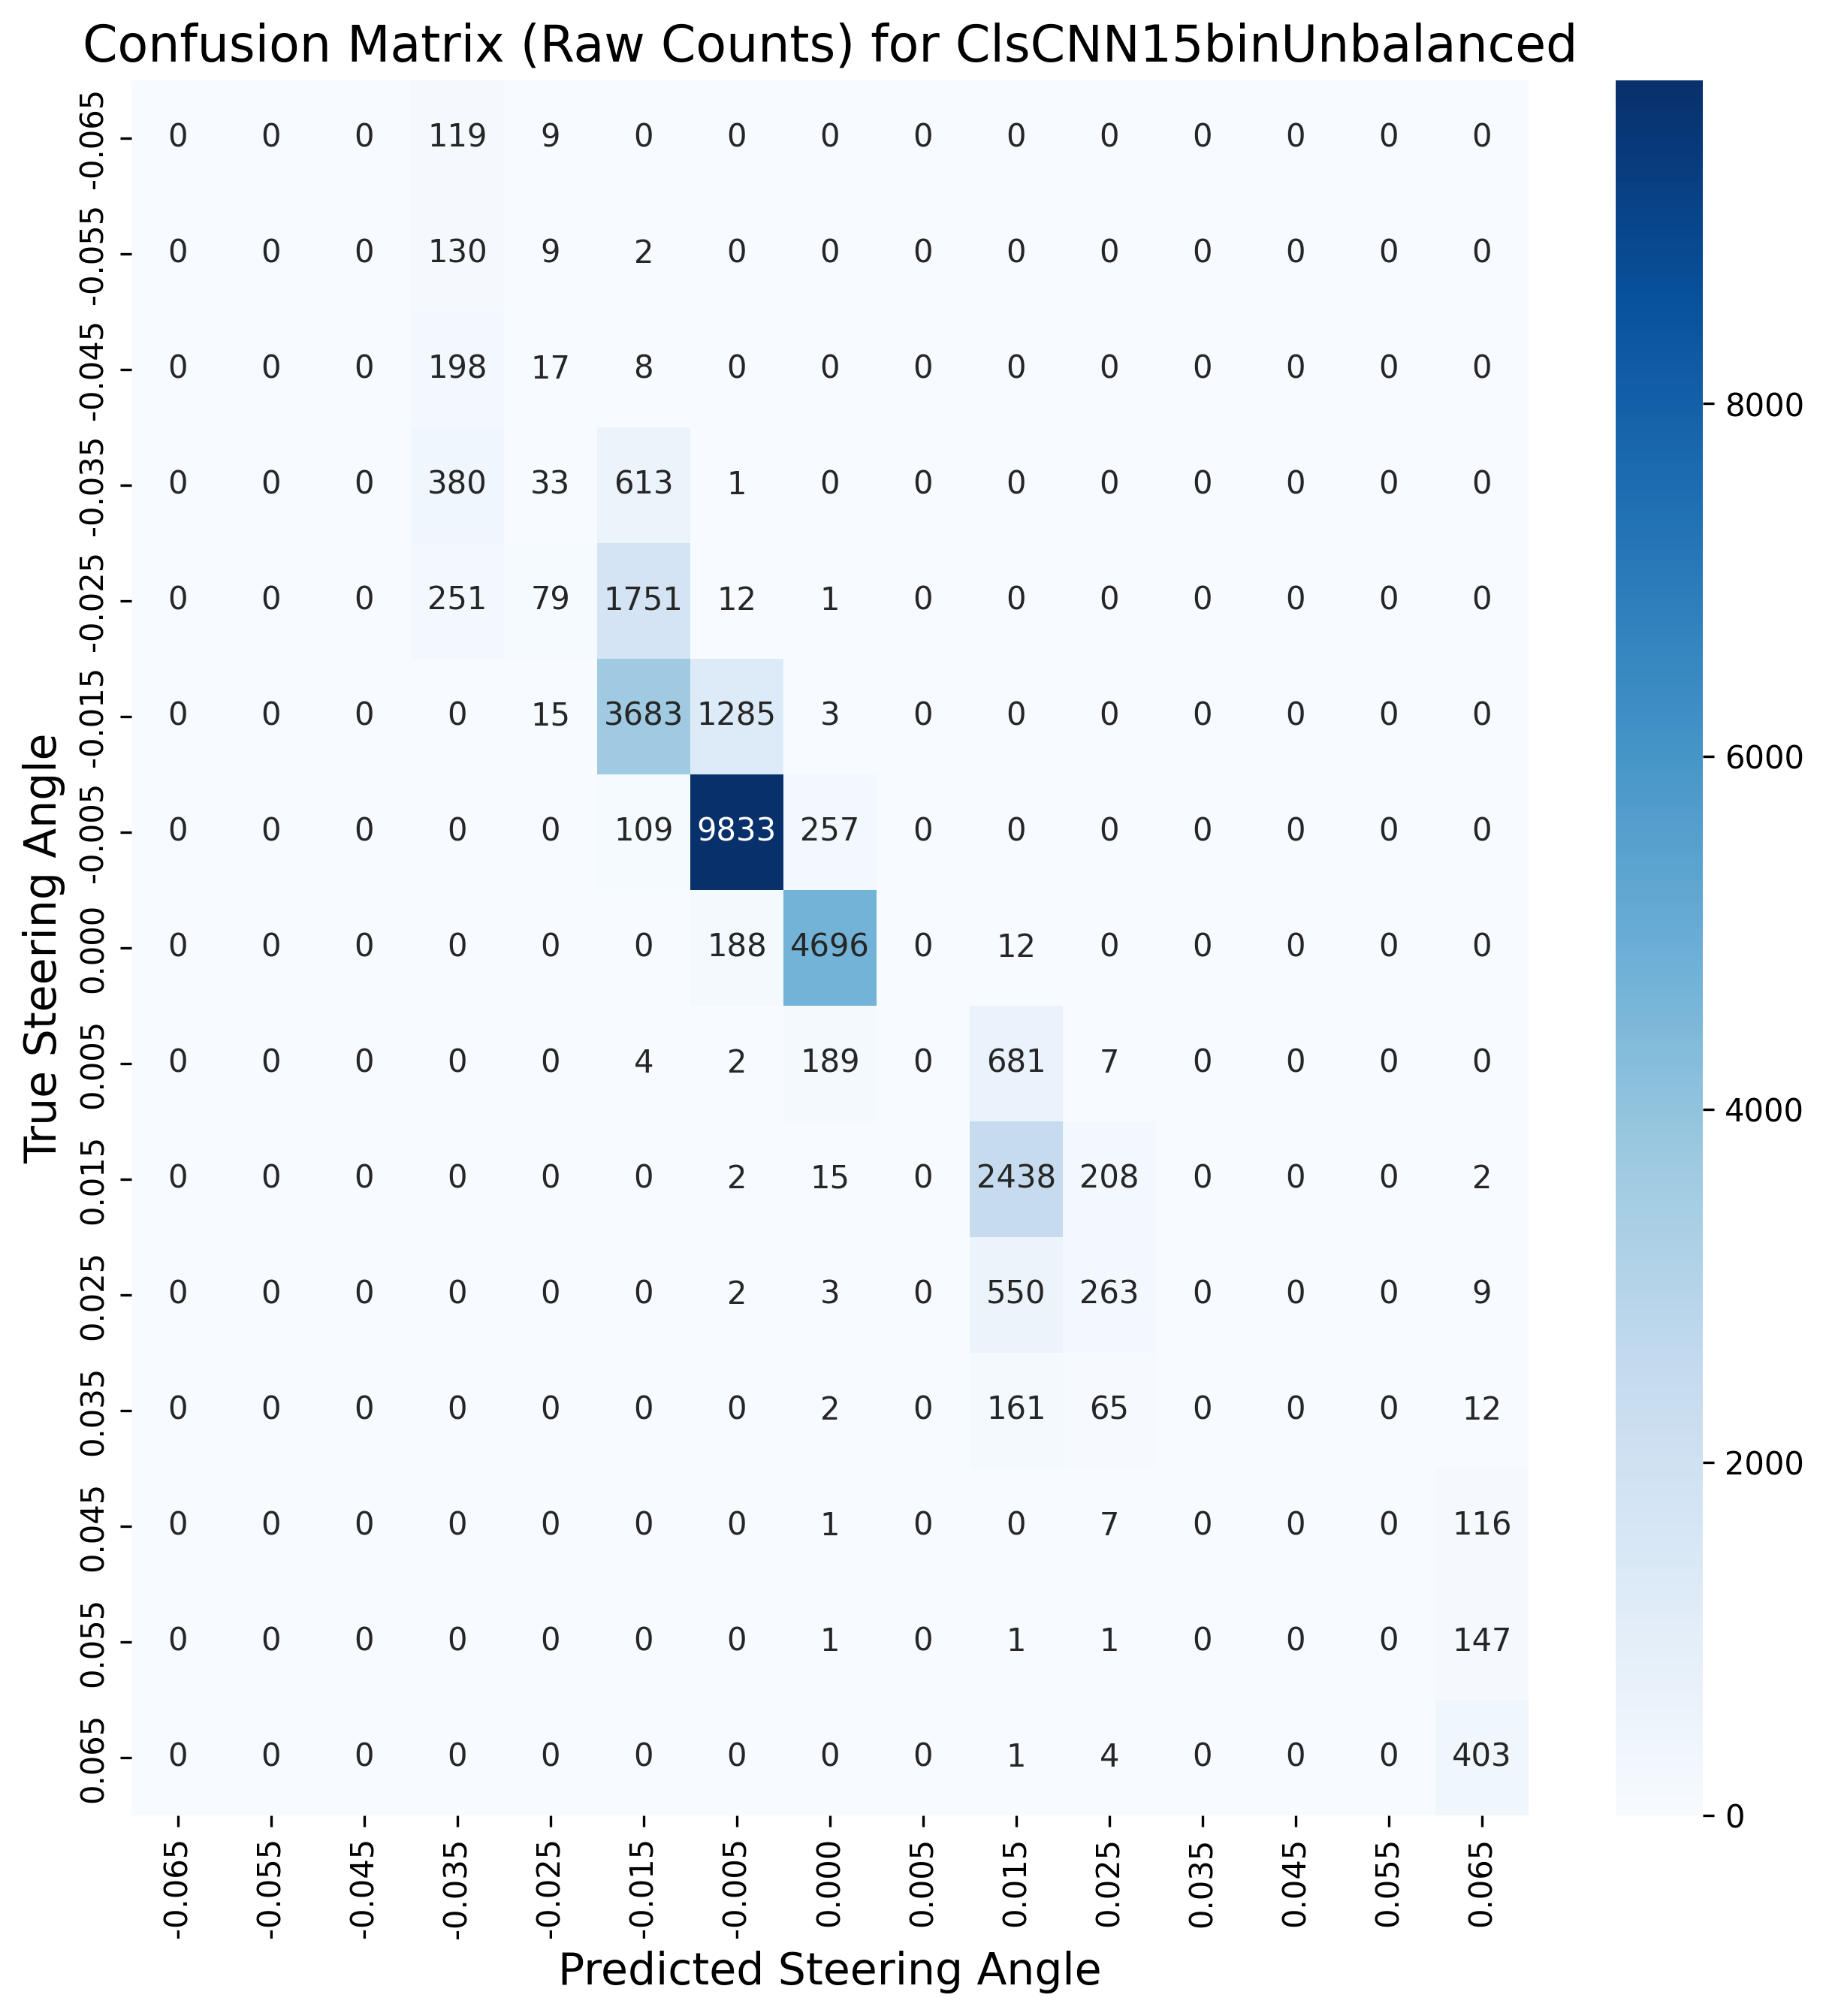
\includegraphics[width=1\linewidth]{Figures/Results/cm_raw_ClsCNN15binUnbalanced.png}
% \caption{ClsCNN15binUnbalanced model raw counts confusion matrix}
% \label{fig:cm_raw_ClsCNN15binUnbalanced}
% \end{figure}

% % ClsCNN15binUnbalanced Normalized Confusion Matrix %

% \begin{figure}[H]
% \centering
% 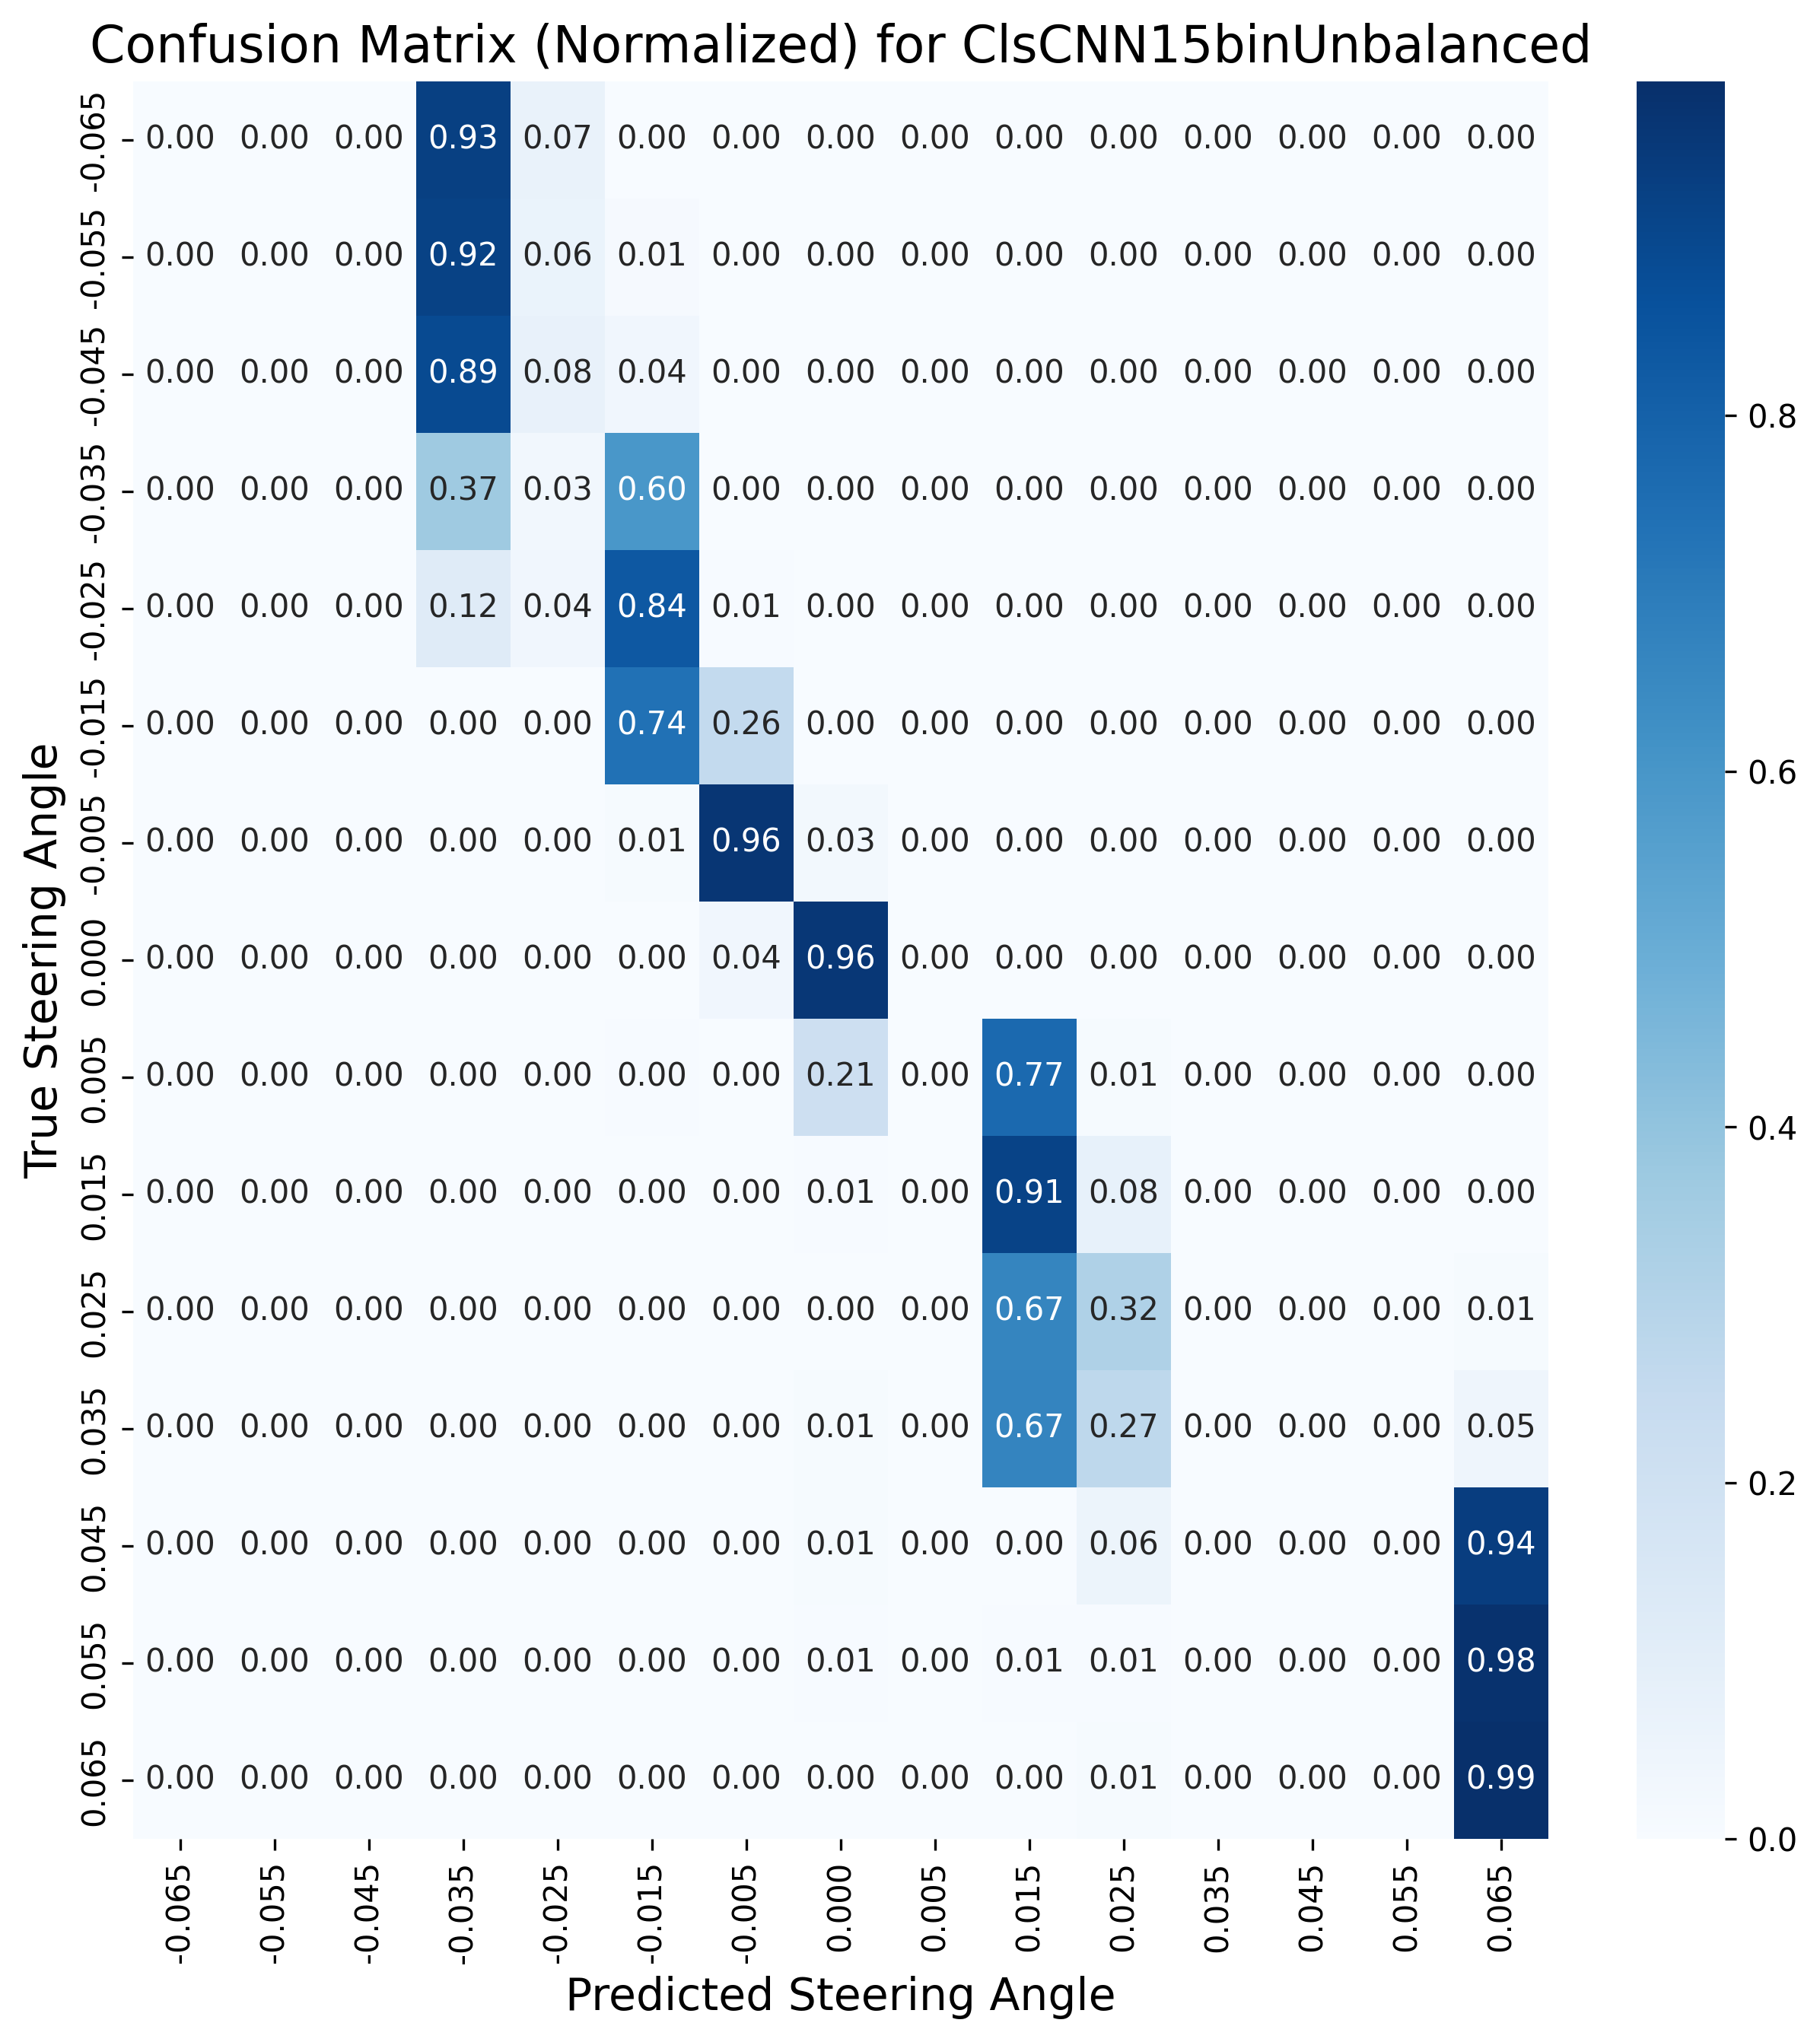
\includegraphics[width=1\linewidth]{Figures/Results/cm_norm_ClsCNN15binUnbalanced.png}
% \caption{ClsCNN15binUnbalanced model normalized confusion matrix}
% \label{fig:cm_norm_ClsCNN15binUnbalanced}
% \end{figure}

% %%%%%%%%%%%%%%%%%%%%%%
% % ClsViT3binBalanced %
% %%%%%%%%%%%%%%%%%%%%%%

% \begin{table}[htbp]
% \centering
% \begin{tabular}{@{}lcccc@{}}
% \toprule
% \textbf{Class} & \textbf{Precision} & \textbf{Recall} & \textbf{F1-Score} & \textbf{Support} \\
% \midrule
% $-0.065$ & 0.98 & 1.00 & 0.99 & 22,460 \\
% $\phantom{-}0.000$ & 1.00 & 0.94 & 0.97 & 22,460 \\
% $\phantom{-}0.065$ & 0.96 & 1.00 & 0.98 & 22,460 \\
% \midrule
% \textbf{Macro Avg} & \textbf{0.98} & \textbf{0.98} & \textbf{0.98} & \textbf{67,380} \\
% \bottomrule
% \end{tabular}
% \caption{Classification performance results for the ClsViT3binBalanced model. The model achieved an overall accuracy of 97.97\% with a mean confidence of 0.9765 across 67,380 test images.}
% \label{tab:clf_report_ClsViT3binBalanced}
% \end{table}

% % ClsViT3binBalanced Raw Counts Confusion Matrix %

% \begin{figure}[H]
% \centering
% 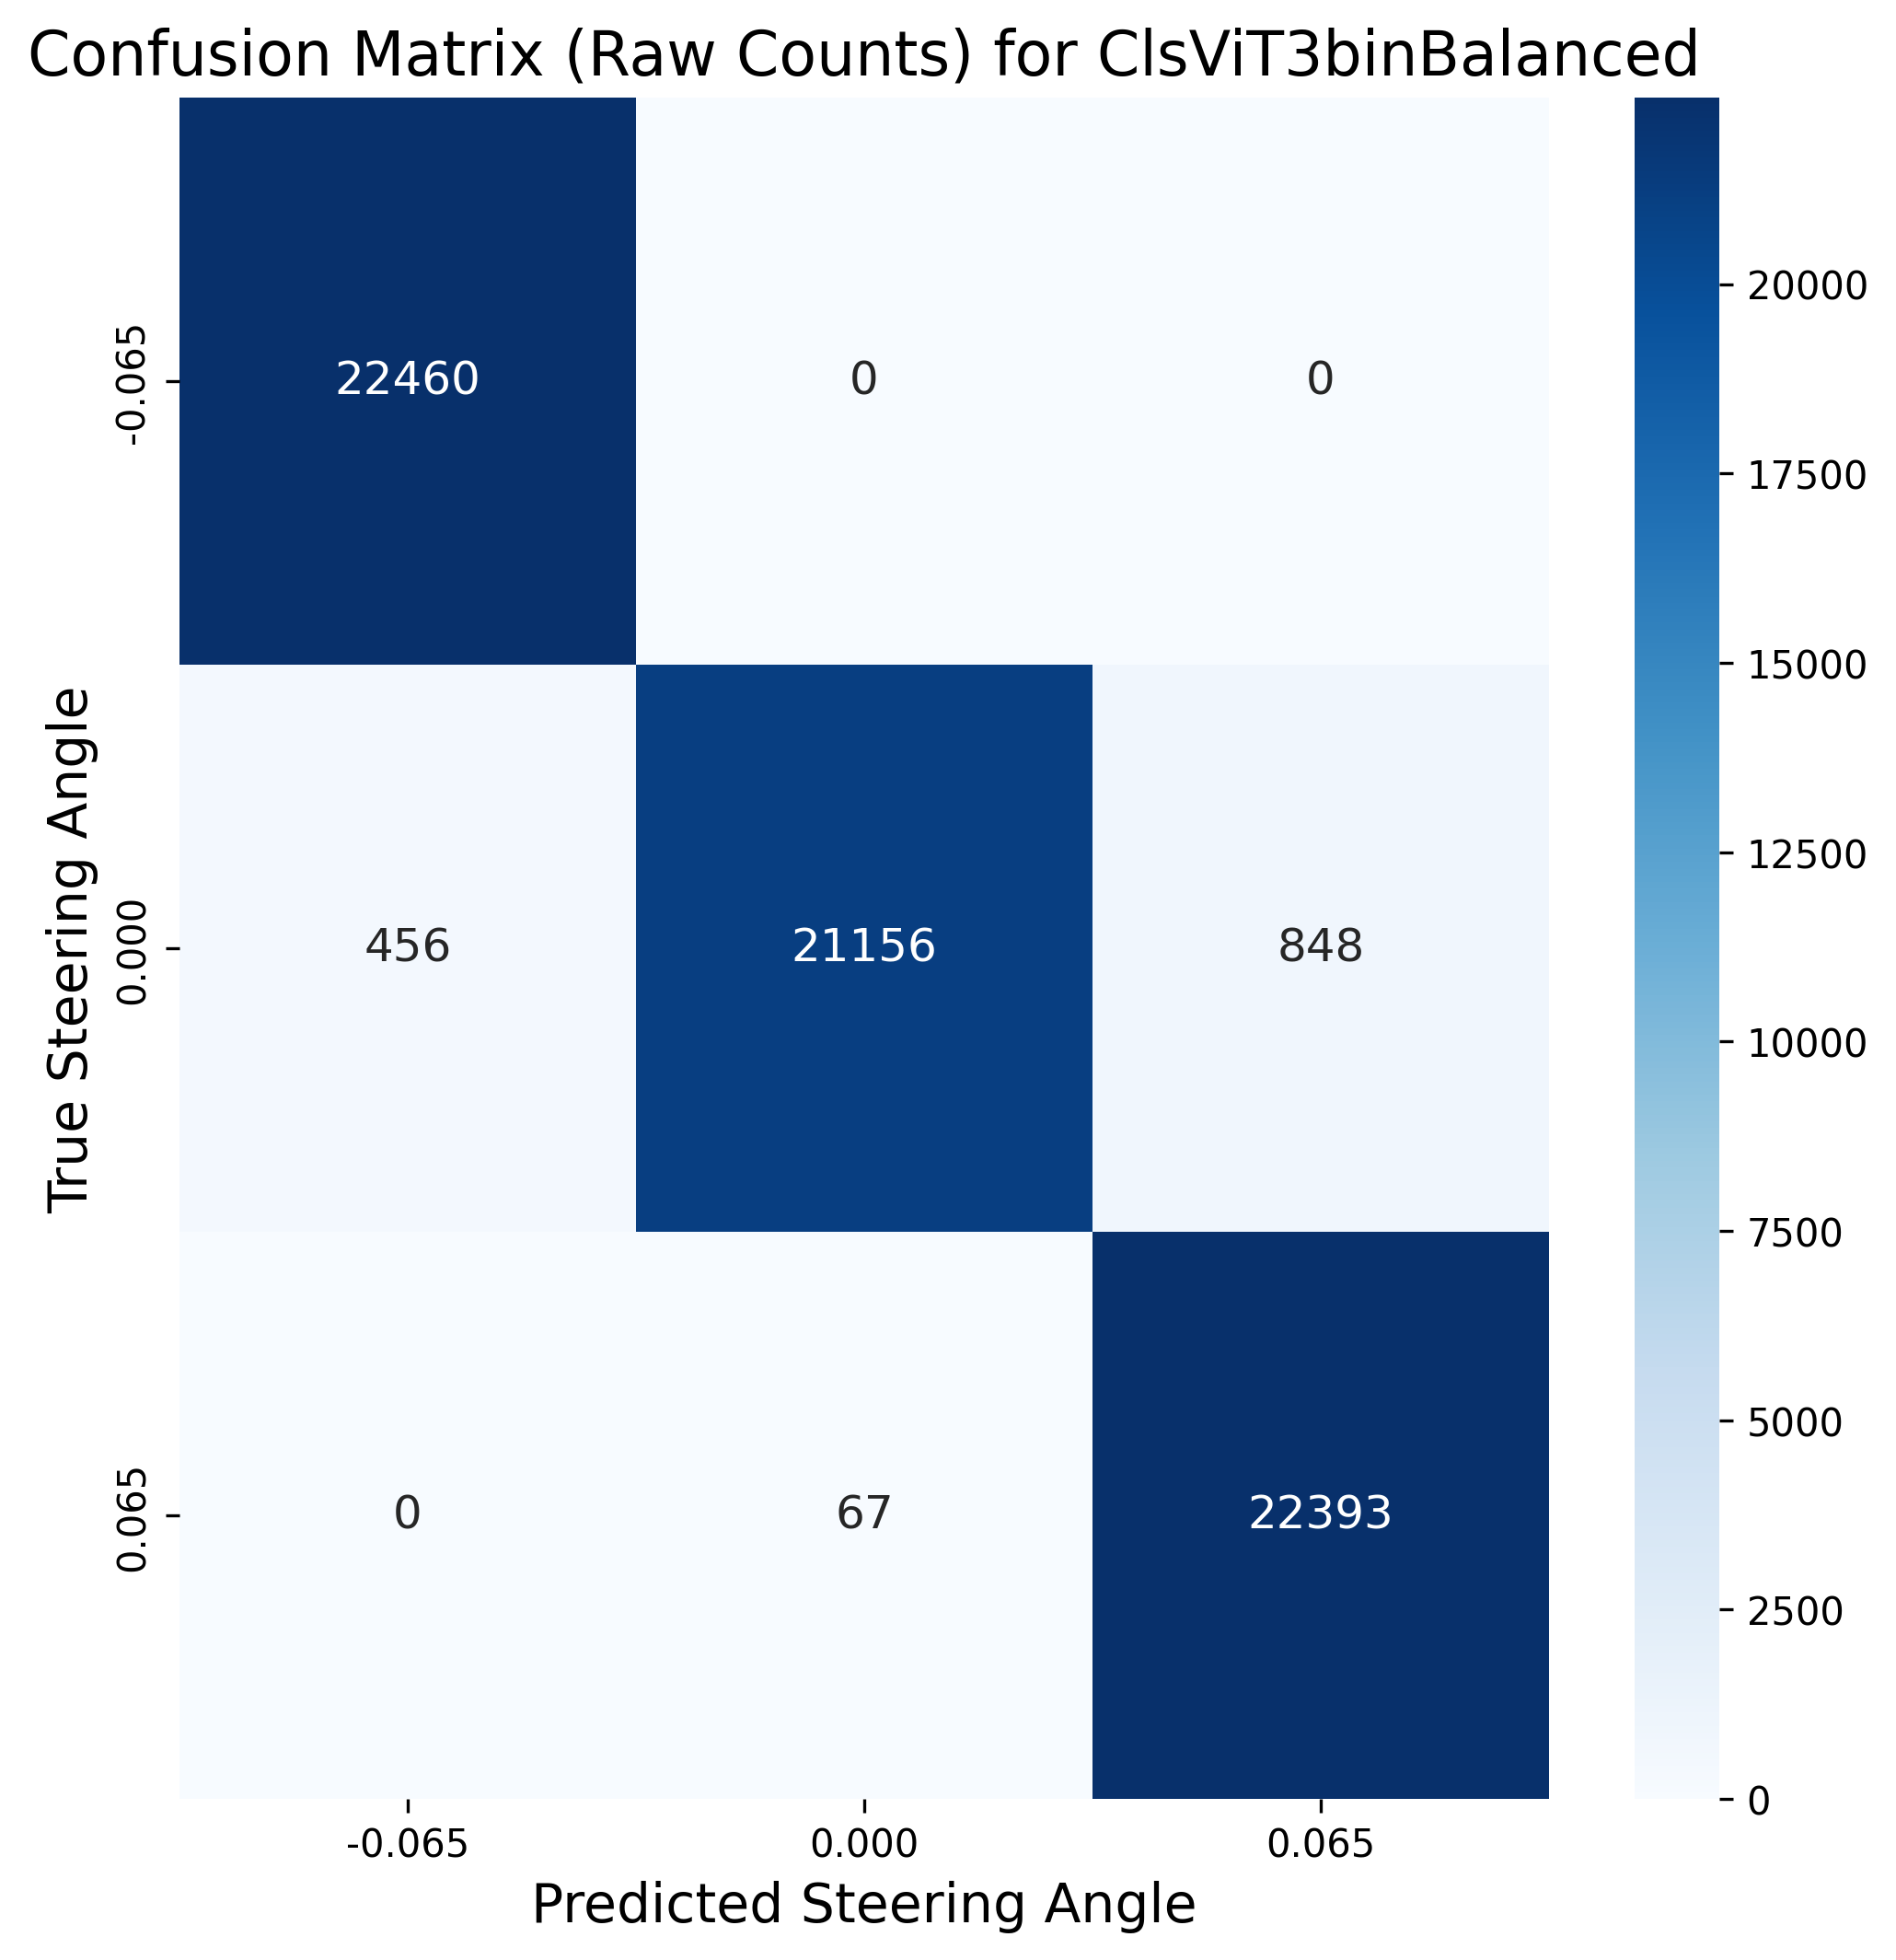
\includegraphics[width=0.65\linewidth]{Figures/Results/cm_raw_ClsViT3binBalanced.png}
% \caption{ClsViT3binBalanced model raw counts confusion matrix}
% \label{fig:cm_raw_ClsViT3binBalanced}
% \end{figure}

% % ClsViT3binBalanced Normalized Confusion Matrix %

% \begin{figure}[H]
% \centering
% 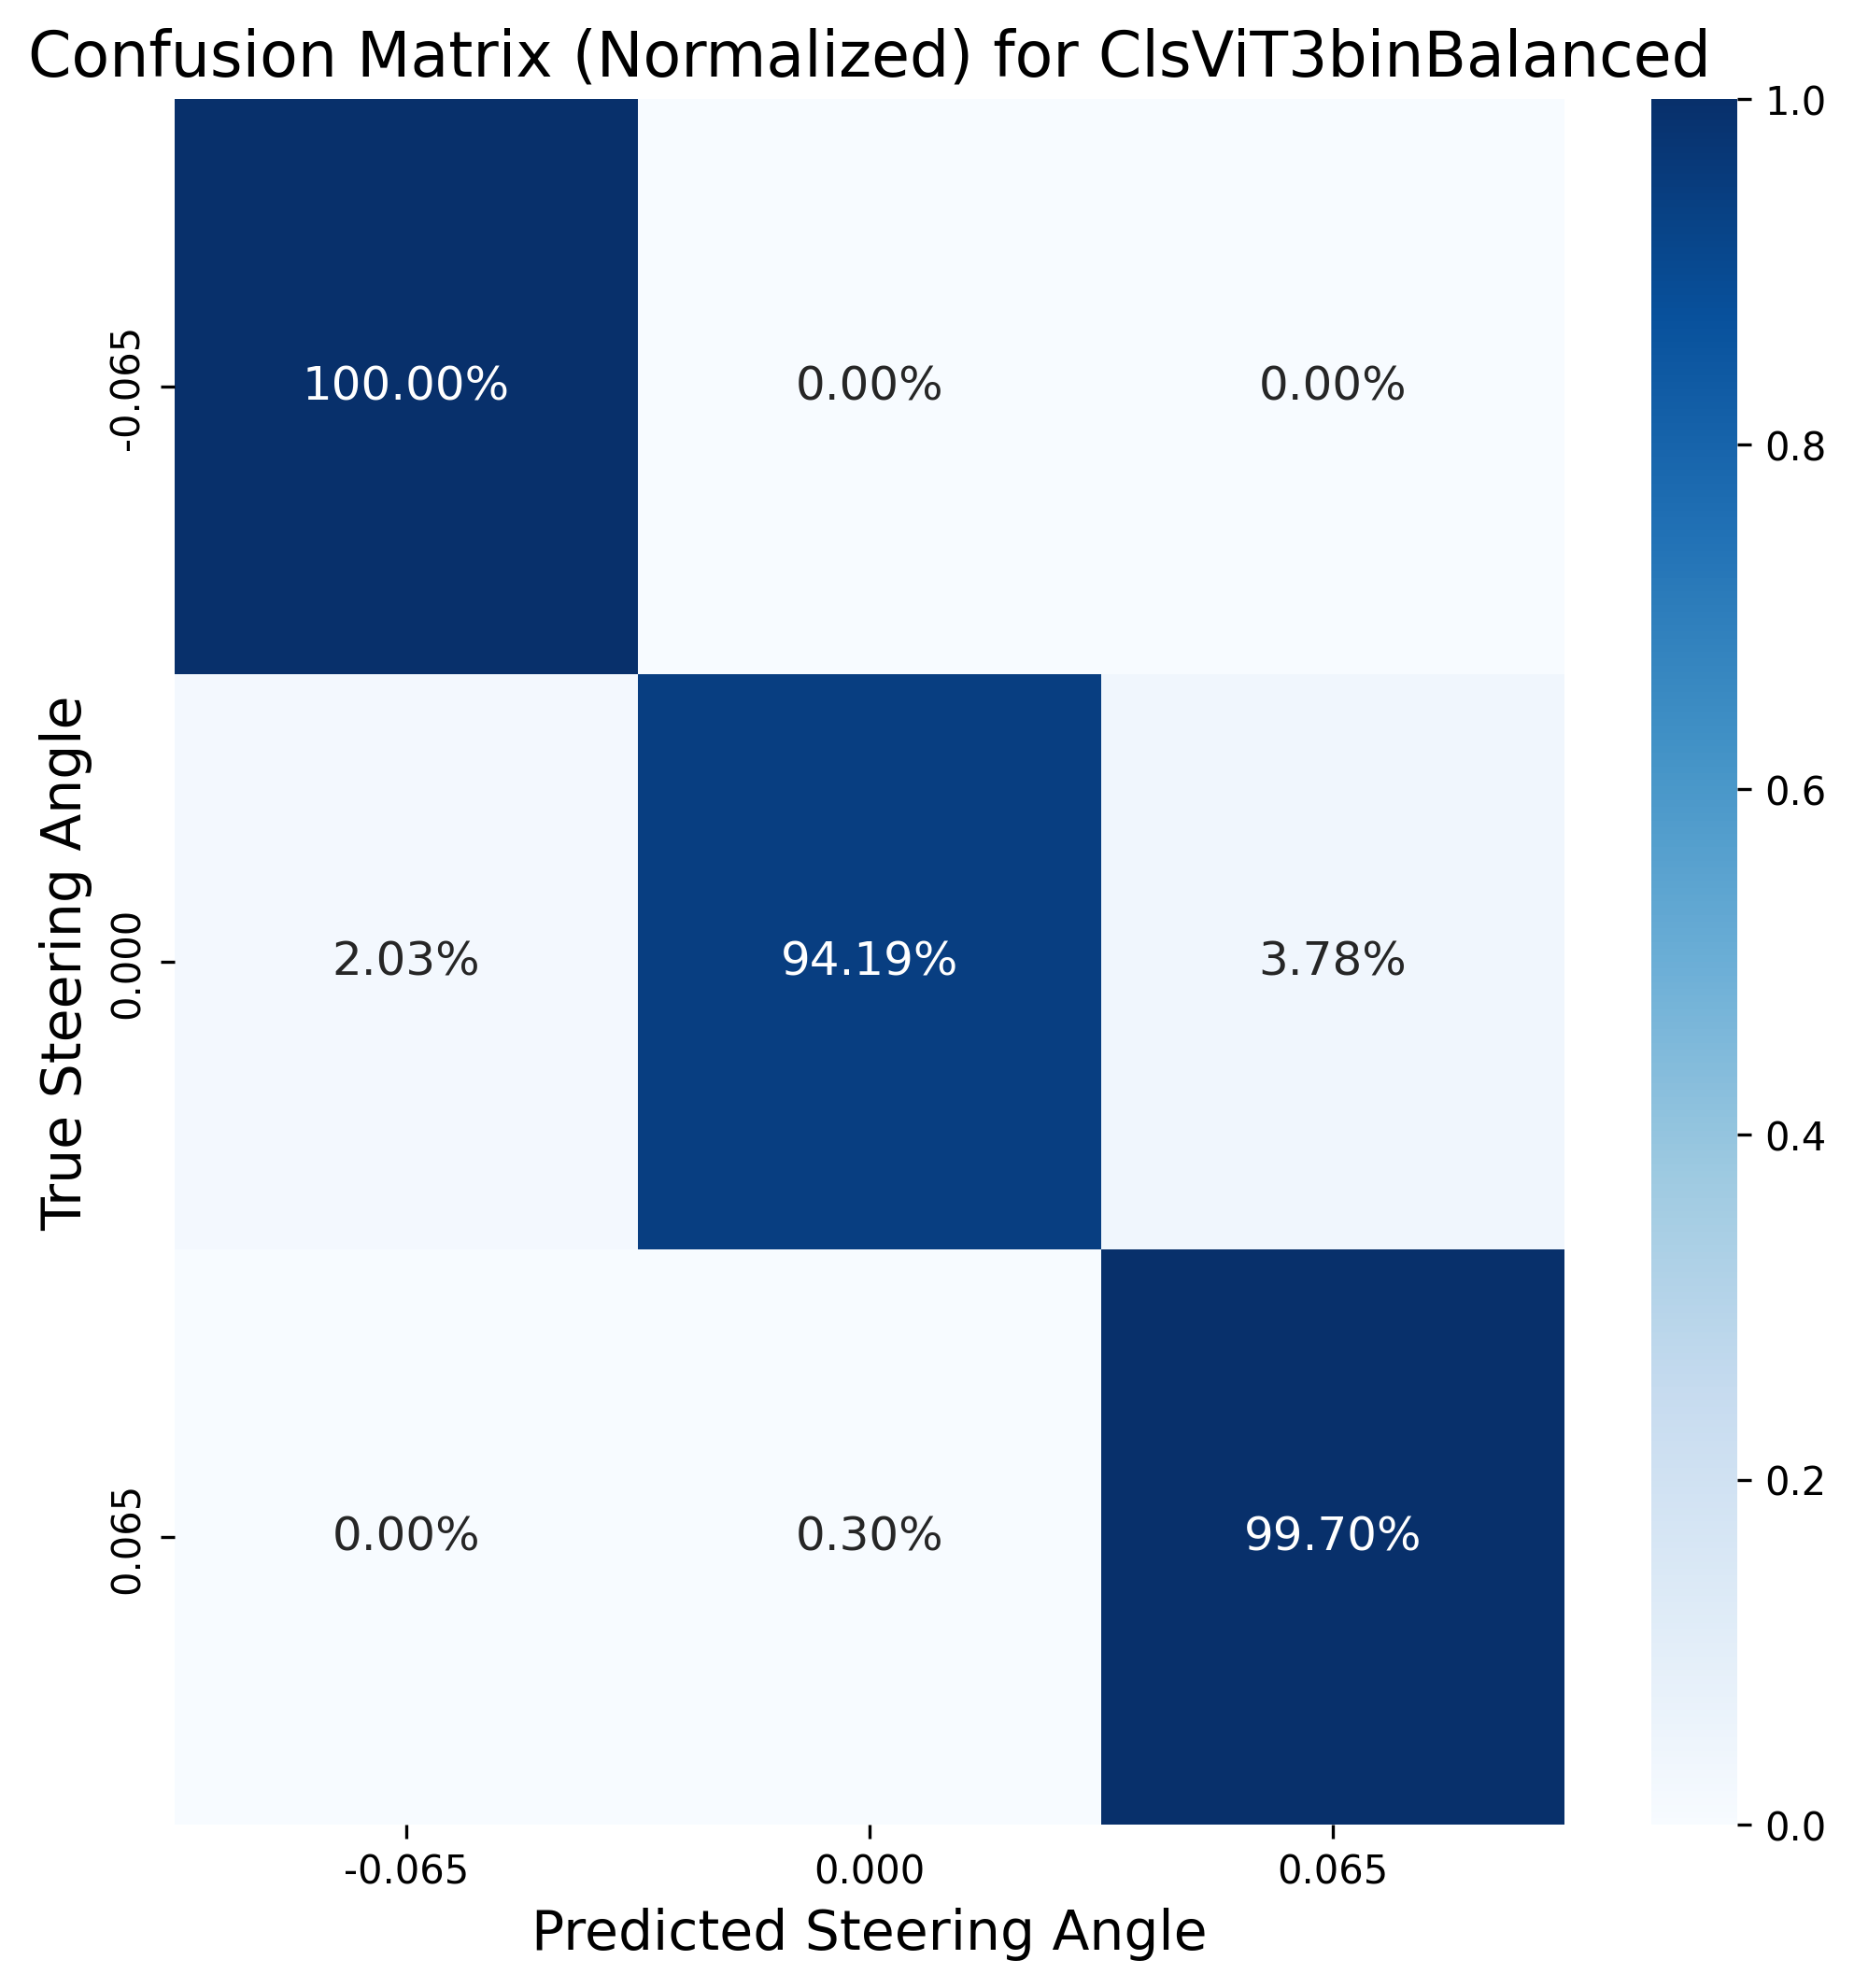
\includegraphics[width=0.65\linewidth]{Figures/Results/cm_norm_ClsViT3binBalanced.png}
% \caption{ClsViT3binBalanced model normalized confusion matrix}
% \label{fig:cm_norm_ClsViT3binBalanced}
% \end{figure}

% %%%%%%%%%%%%%%%%%%%%%%%%
% % ClsViT3binUnbalanced %
% %%%%%%%%%%%%%%%%%%%%%%%%

% \begin{table}[htbp]
% \centering
% \begin{tabular}{@{}lcccc@{}}
% \toprule
% \textbf{Class} & \textbf{Precision} & \textbf{Recall} & \textbf{F1-Score} & \textbf{Support} \\
% \midrule
% $-0.065$ & 0.82 & 0.66 & 0.73 & 1,422 \\
% $\phantom{-}0.000$ & 0.94 & 0.98 & 0.96 & 22,460 \\
% $\phantom{-}0.065$ & 0.86 & 0.67 & 0.75 & 3,059 \\
% \midrule
% \textbf{Macro Avg} & \textbf{0.87} & \textbf{0.77} & \textbf{0.81} & \textbf{26,941} \\
% \bottomrule
% \end{tabular}
% \caption{Classification performance results for the ClsViT3binUnbalanced model. The model achieved an overall accuracy of 92.50\% with a mean confidence of 0.9211 across 26,941 test images.}
% \label{tab:clf_report_ClsViT3binUnbalanced}
% \end{table}

% % ClsViT3binUnbalanced Raw Counts Confusion Matrix %

% \begin{figure}[H]
% \centering
% 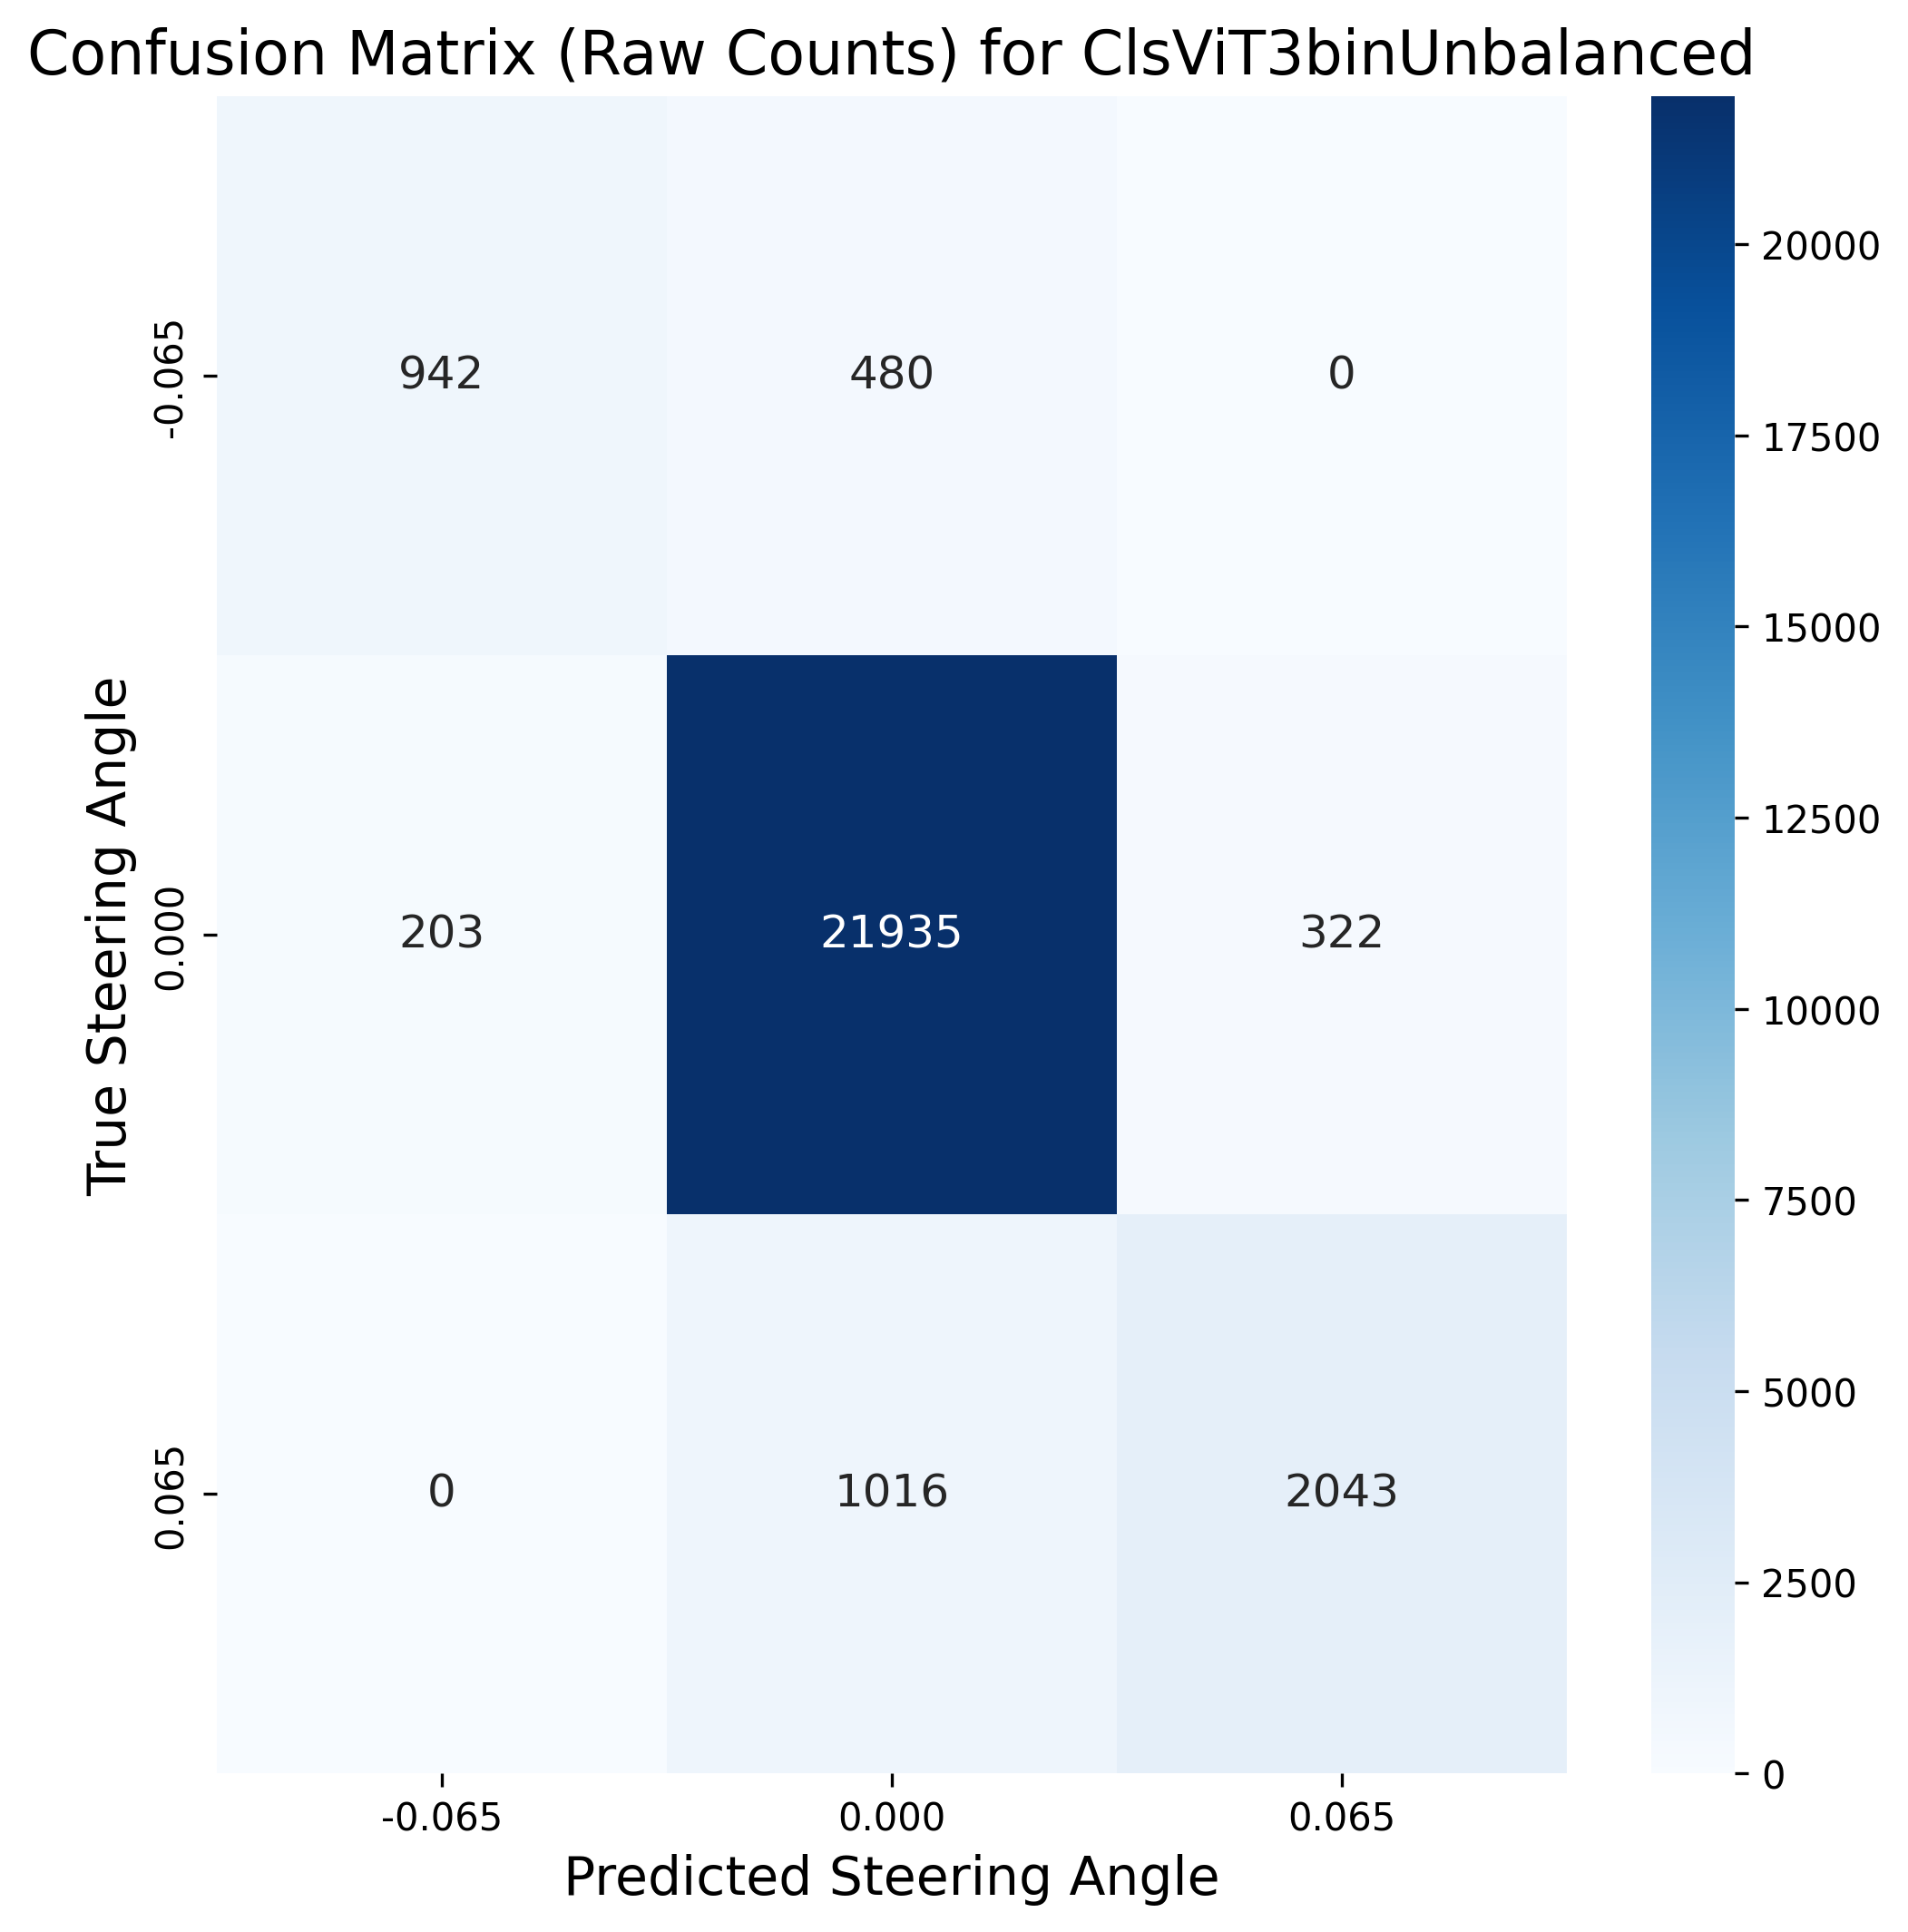
\includegraphics[width=0.65\linewidth]{Figures/Results/cm_raw_ClsViT3binUnbalanced.png}
% \caption{ClsViT3binUnbalanced model raw counts confusion matrix}
% \label{fig:cm_raw_ClsViT3binUnbalanced}
% \end{figure}

% % ClsViT3binUnbalanced Normalized Confusion Matrix %

% \begin{figure}[H]
% \centering
% 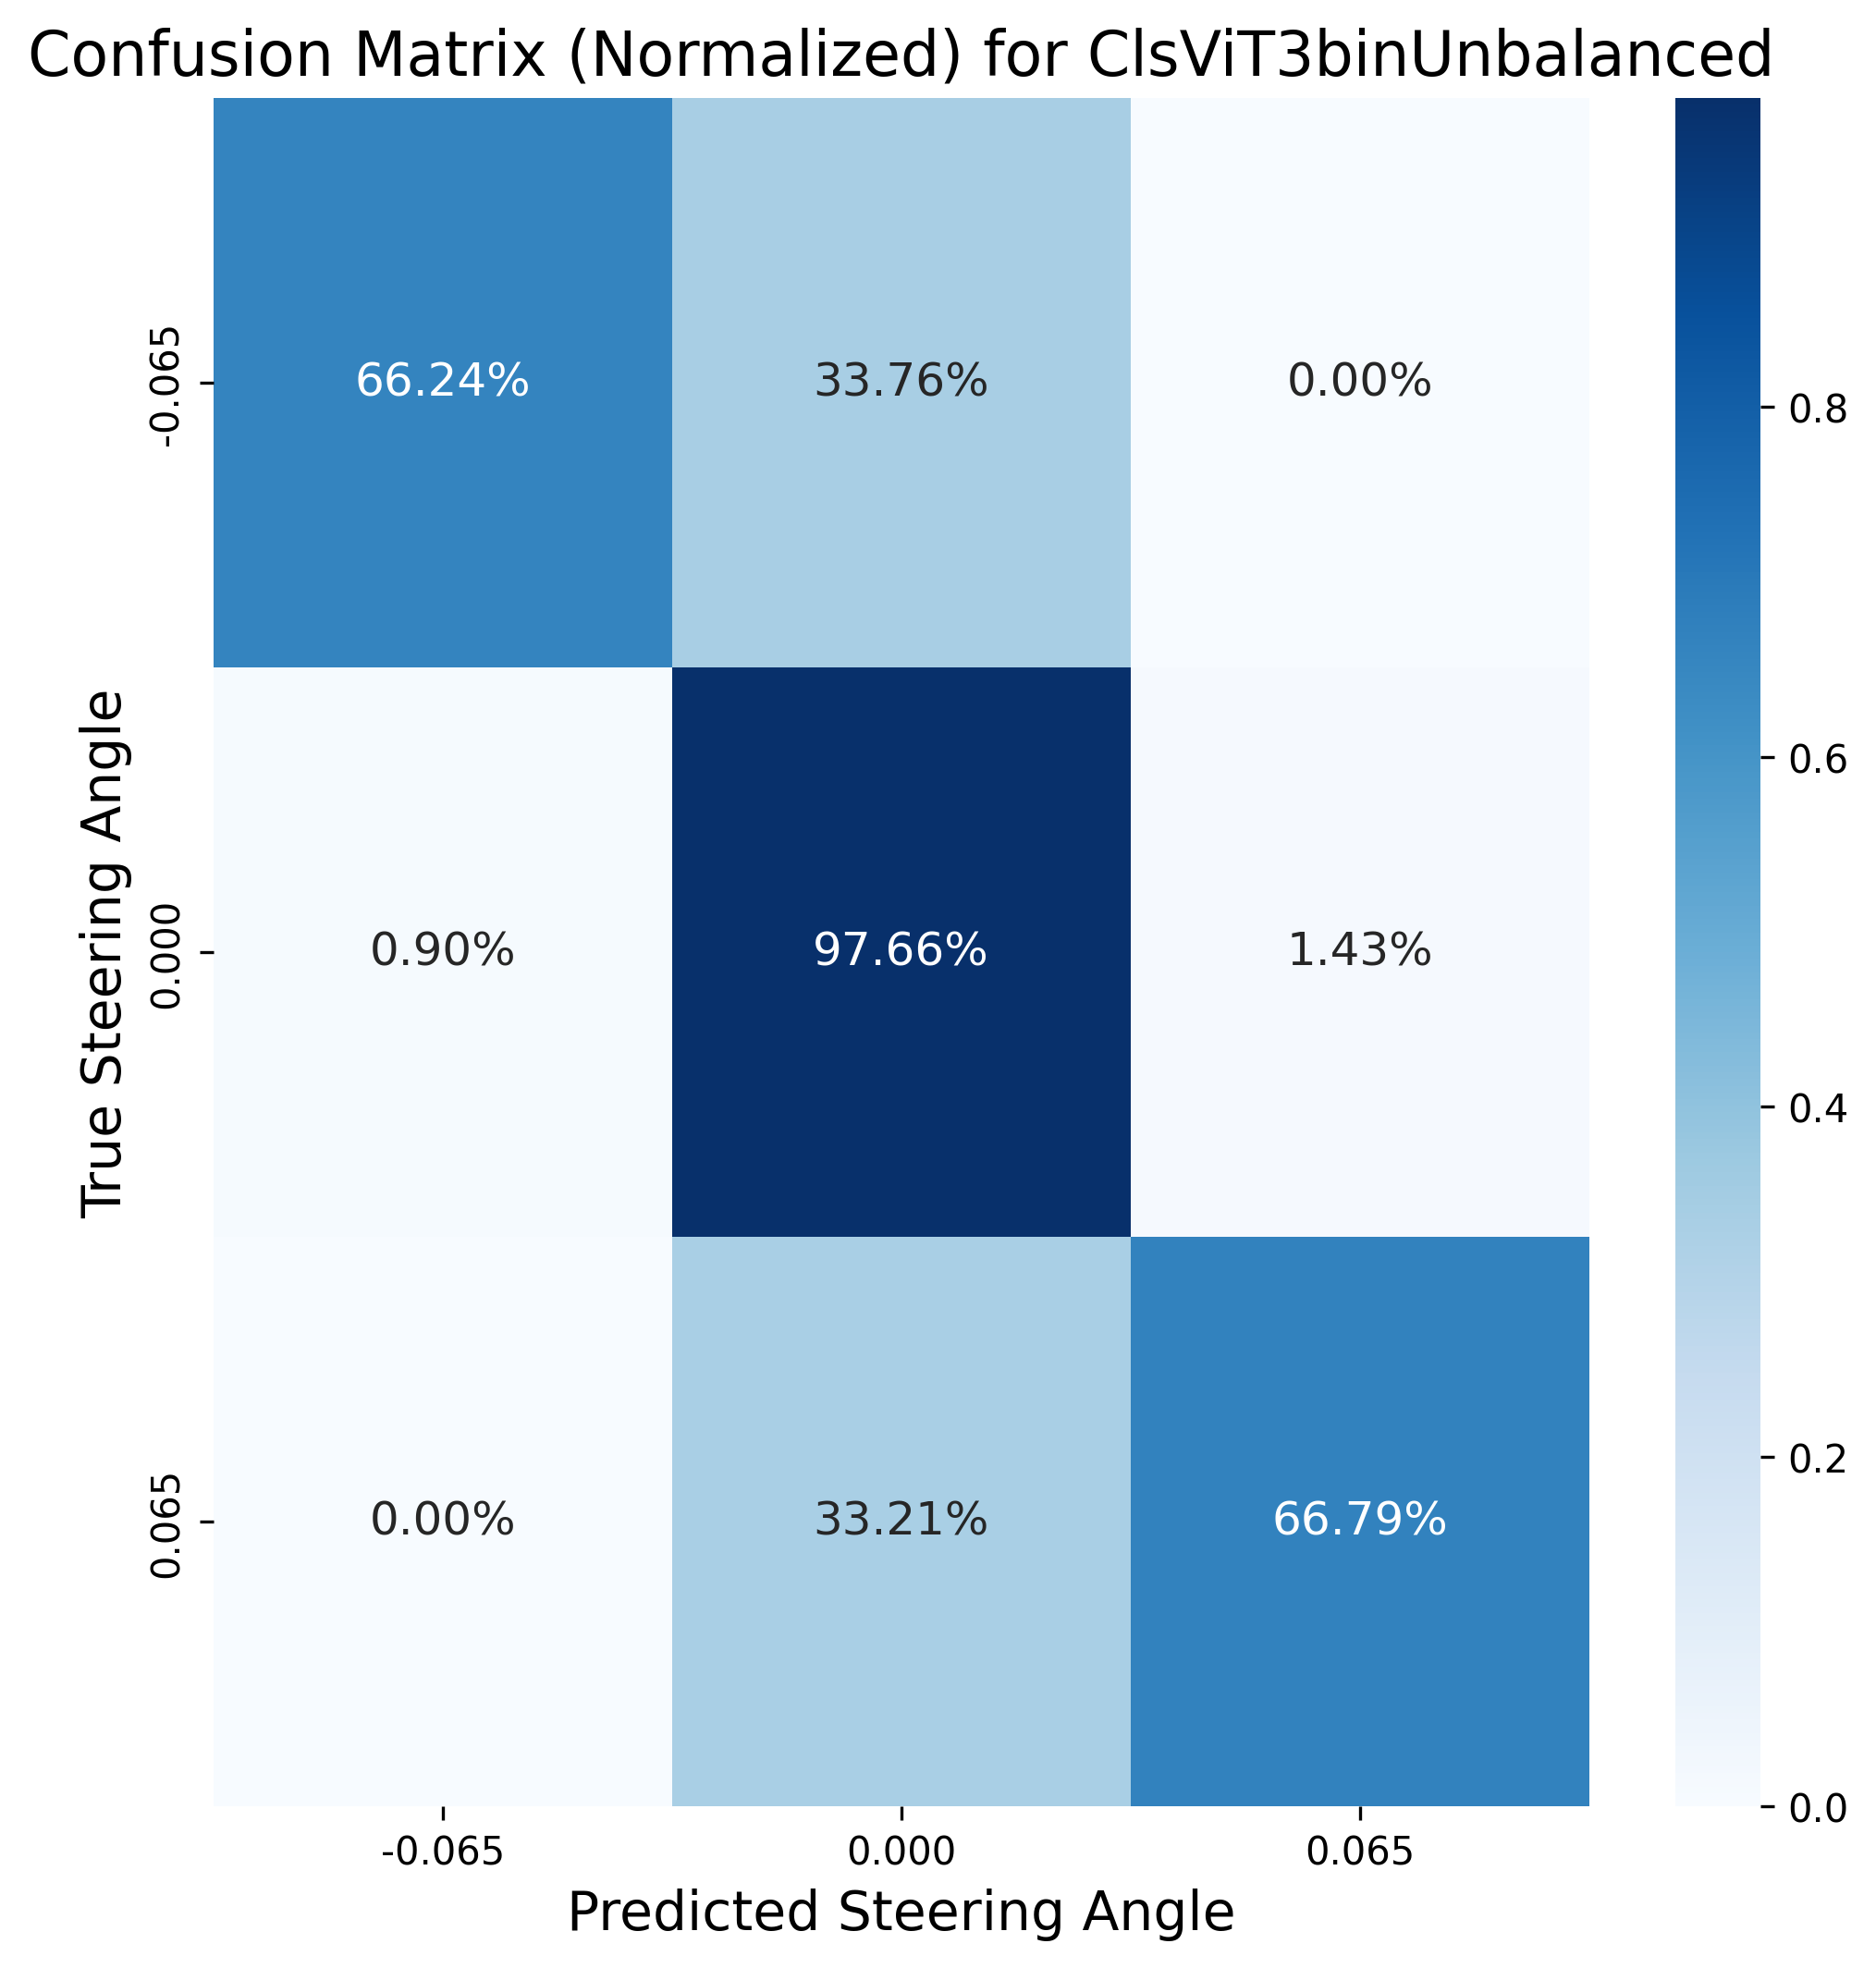
\includegraphics[width=0.65\linewidth]{Figures/Results/cm_norm_ClsViT3binUnbalanced.png}
% \caption{ClsViT3binUnbalanced model normalized confusion matrix}
% \label{fig:cm_norm_ClsViT3binUnbalanced}
% \end{figure}

% %%%%%%%%%%%%%%%%%%%%%%%%
% % ClsVLM3binUnbalanced %
% %%%%%%%%%%%%%%%%%%%%%%%%

% % ClsVLM3binUnbalanced %

% \begin{table}[htbp]
% \centering
% \begin{tabular}{@{}lcccc@{}}
% \toprule
% \textbf{Class} & \textbf{Precision} & \textbf{Recall} & \textbf{F1-Score} & \textbf{Support} \\
% \midrule
% $-0.065$ & 0.50 & 0.19 & 0.27 & 1,422 \\
% $\phantom{-}0.000$ & 0.86 & 0.99 & 0.92 & 22,460 \\
% $\phantom{-}0.065$ & 0.91 & 0.17 & 0.28 & 3,059 \\
% \midrule
% \textbf{Macro Avg} & \textbf{0.76} & \textbf{0.45} & \textbf{0.49} & \textbf{26,941} \\
% \bottomrule
% \end{tabular}
% \caption{Classification performance results for the ClsVLM3binUnbalanced model. The model achieved an overall accuracy of 85.08\% with a mean confidence of 0.9062 across 26,941 test images.}
% \label{tab:clf_report_ClsVLM3binUnbalanced}
% \end{table}

% % ClsVLM3binUnbalanced Raw Counts Confusion Matrix %

% \begin{figure}[H]
% \centering
% 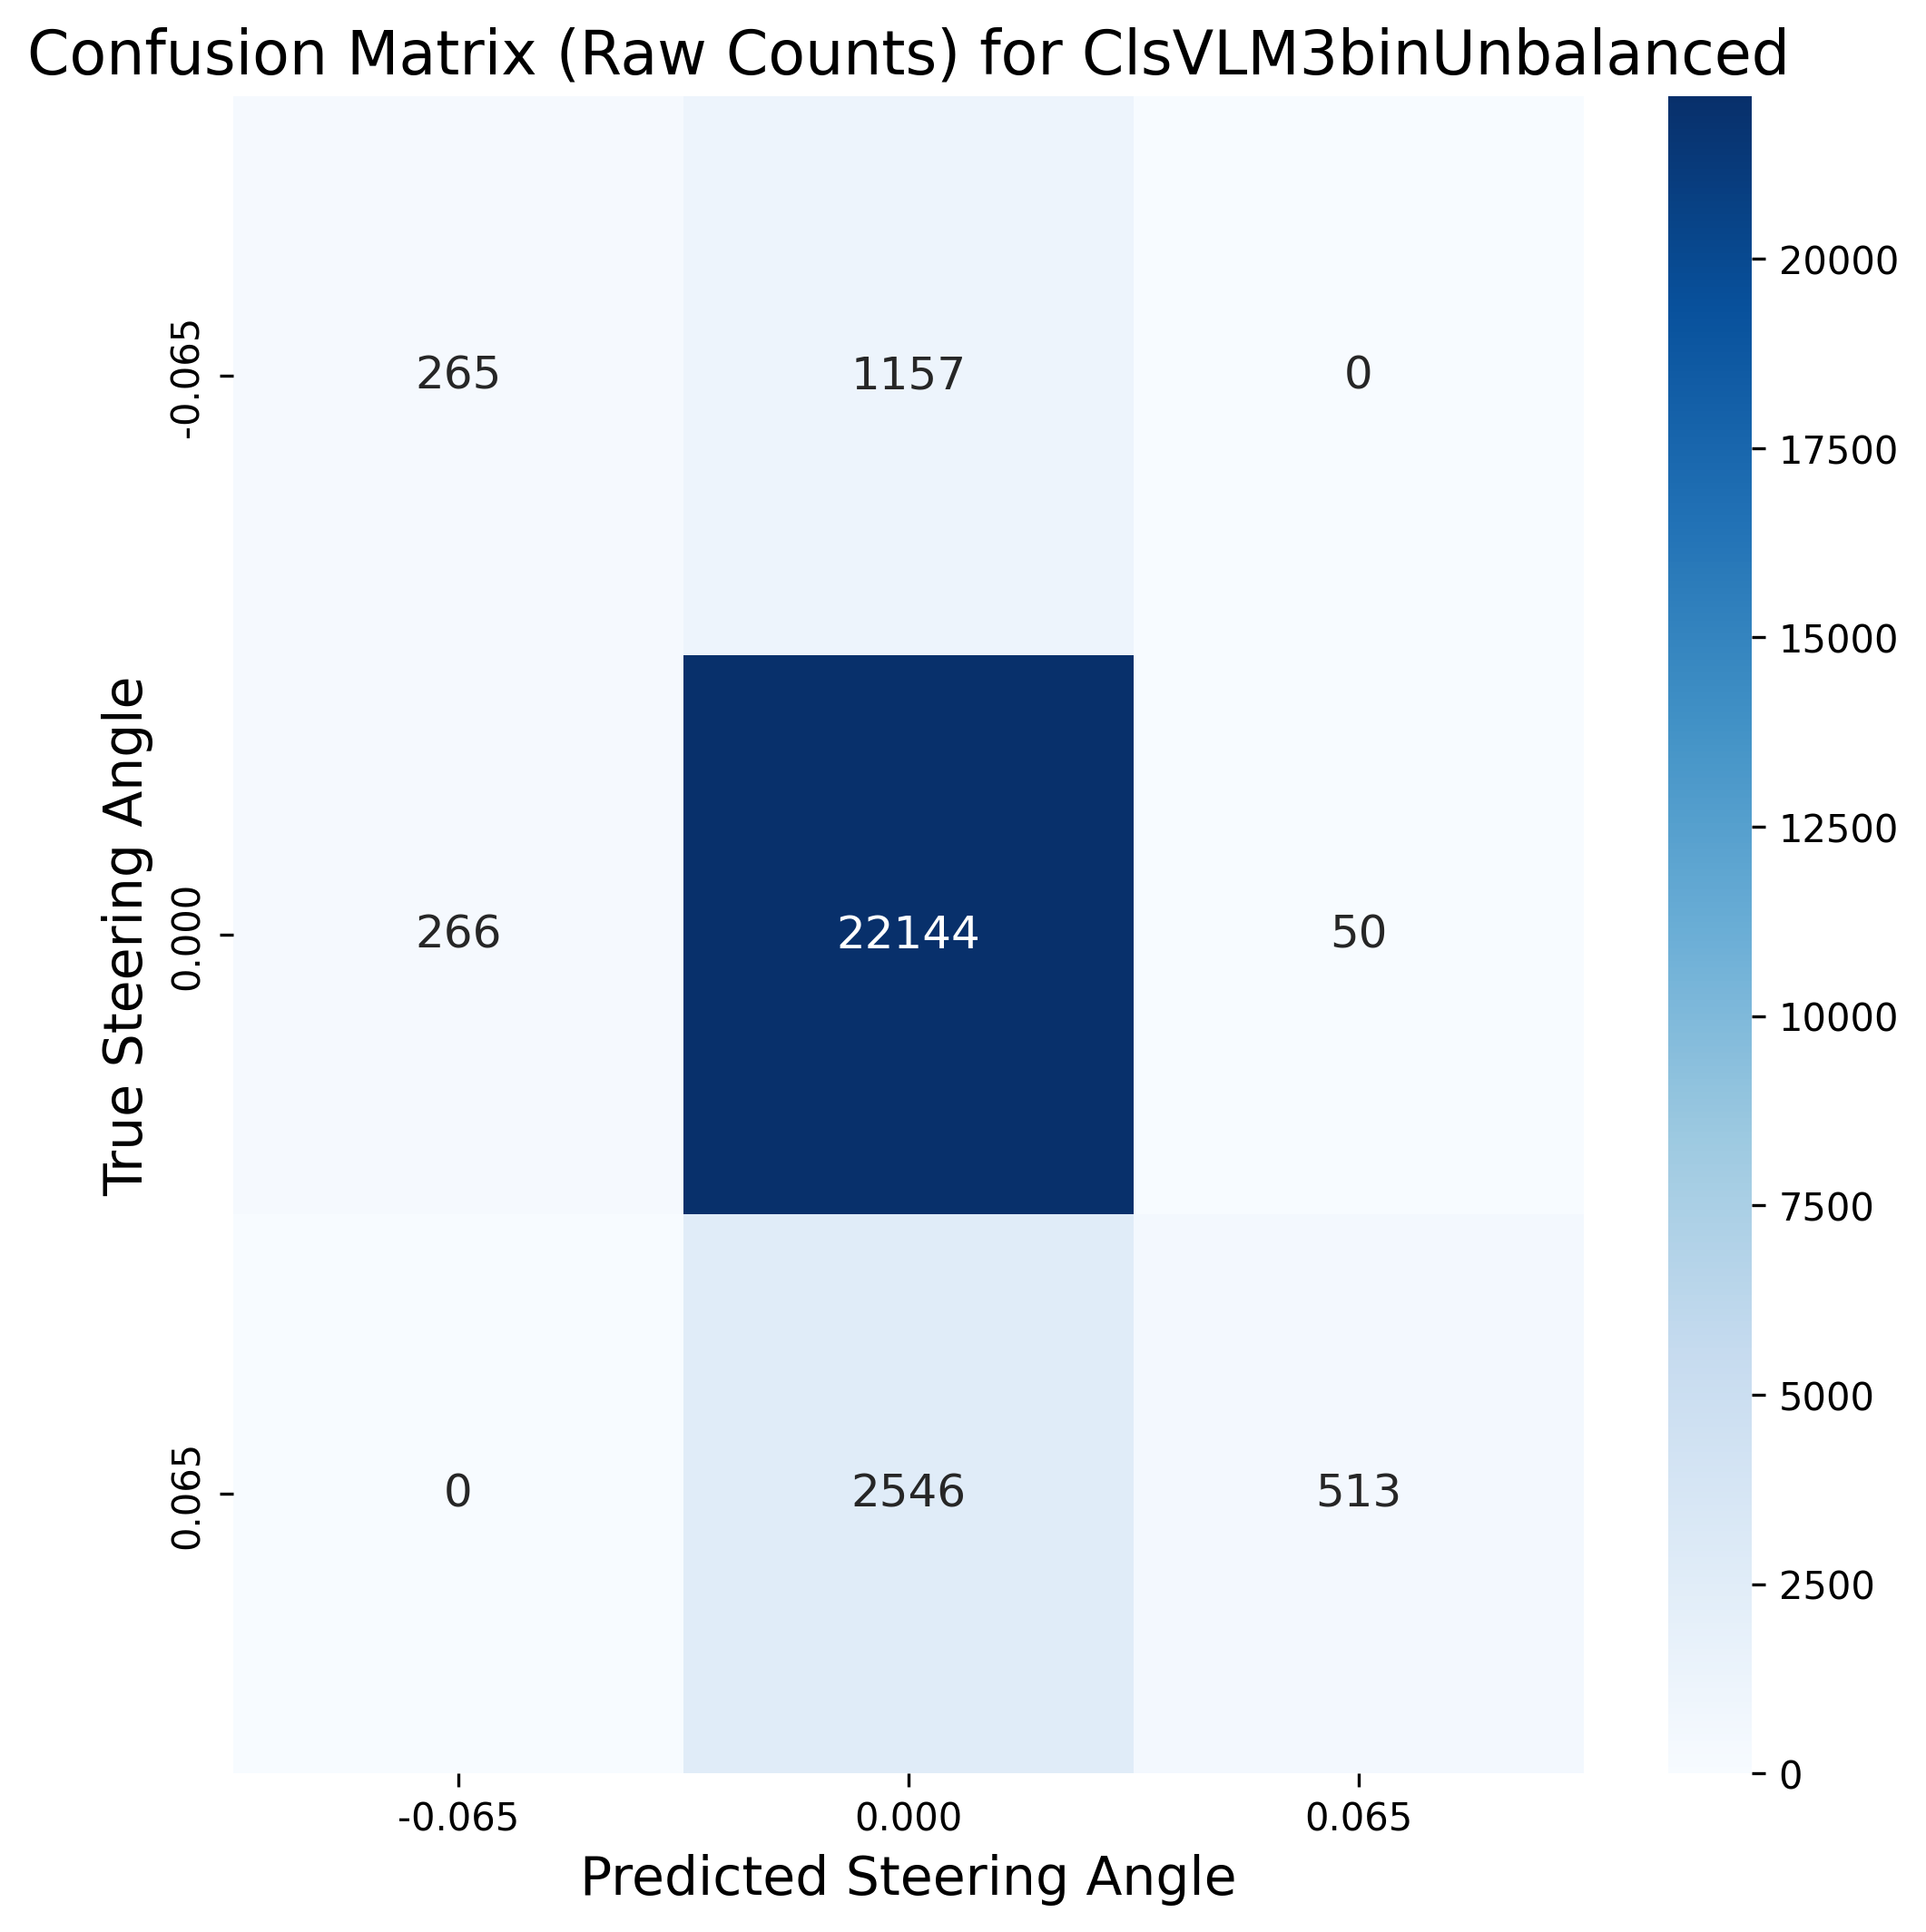
\includegraphics[width=0.65\linewidth]{Figures/Results/cm_raw_ClsVLM3binUnbalanced.png}
% \caption{ClsVLM3binUnbalanced model raw counts confusion matrix}
% \label{fig:cm_raw_ClsVLM3binUnbalanced}
% \end{figure}

% % ClsVLM3binUnbalanced Normalized Confusion Matrix %

% \begin{figure}[H]
% \centering
% \includegraphics[width=0.65\linewidth]{Figures/Results/cm_norm_ClsVLM3binUnbalanced.png}
% \caption{ClsVLM3binUnbalanced model normalized confusion matrix}
% \label{fig:cm_norm_ClsVLM3binUnbalanced}
% \end{figure}

% %%%%%%%%%%%%%%%%%%%%%%
% % ClsViT5binBalanced %
% %%%%%%%%%%%%%%%%%%%%%%

% \begin{table}[htbp]
% \centering
% \begin{tabular}{@{}lcccc@{}}
% \toprule
% \textbf{Class} & \textbf{Precision} & \textbf{Recall} & \textbf{F1-Score} & \textbf{Support} \\
% \midrule
% $-0.065$ & 0.99 & 1.00 & 1.00 & 15,839 \\
% $-0.015$ & 0.96 & 0.99 & 0.97 & 15,839 \\
% $\phantom{-}0.000$ & 0.99 & 0.95 & 0.97 & 15,839 \\
% $\phantom{-}0.015$ & 1.00 & 0.95 & 0.97 & 15,839 \\
% $\phantom{-}0.065$ & 0.96 & 1.00 & 0.98 & 15,839 \\
% \midrule
% \textbf{Macro Avg} & \textbf{0.98} & \textbf{0.98} & \textbf{0.98} & \textbf{79,195} \\
% \bottomrule
% \end{tabular}
% \caption{Classification performance results for the ClsViT5binBalanced model. The model achieved an overall accuracy of 97.77\% with a mean confidence of 0.9779 across 79,195 test images.}
% \label{tab:clf_report_ClsViT5binBalanced}
% \end{table}

% % ClsViT5binBalanced Raw Counts Confusion Matrix %

% \begin{figure}[H]
% \centering
% \includegraphics[width=0.65\linewidth]{Figures/Results/cm_raw_ClsViT5binBalanced.png}
% \caption{ClsViT5binBalanced model raw counts confusion matrix}
% \label{fig:cm_raw_ClsViT5binBalanced}
% \end{figure}

% % ClsViT5binBalanced Normalized Confusion Matrix %

% \begin{figure}[H]
% \centering
% \includegraphics[width=0.65\linewidth]{Figures/Results/cm_norm_ClsViT5binBalanced.png}
% \caption{ClsViT5binBalanced model normalized confusion matrix}
% \label{fig:cm_norm_ClsViT5binBalanced}
% \end{figure}

% %%%%%%%%%%%%%%%%%%%%%%%%
% % ClsViT5binUnbalanced %
% %%%%%%%%%%%%%%%%%%%%%%%%

% \begin{table}[htbp]
% \centering
% \begin{tabular}{@{}lcccc@{}}
% \toprule
% \textbf{Class} & \textbf{Precision} & \textbf{Recall} & \textbf{F1-Score} & \textbf{Support} \\
% \midrule
% $-0.065$ & 0.92 & 0.94 & 0.93 & 401 \\
% $-0.015$ & 0.89 & 0.97 & 0.93 & 5,843 \\
% $\phantom{-}0.000$ & 0.99 & 0.96 & 0.97 & 15,839 \\
% $\phantom{-}0.015$ & 0.92 & 0.97 & 0.94 & 3,972 \\
% $\phantom{-}0.065$ & 0.90 & 0.67 & 0.77 & 936 \\
% \midrule
% \textbf{Macro Avg} & \textbf{0.92} & \textbf{0.90} & \textbf{0.91} & \textbf{26,991} \\
% \bottomrule
% \end{tabular}
% \caption{Classification performance results for the ClsViT5binUnbalanced model. The model achieved an overall accuracy of 94.97\% with a mean confidence of 0.9435 across 26,991 test images.}
% \label{tab:clf_report_ClsViT5binUnbalanced}
% \end{table}

% % ClsViT5binUnbalanced Raw Counts Confusion Matrix %

% \begin{figure}[H]
% \centering
% \includegraphics[width=0.65\linewidth]{Figures/Results/cm_raw_ClsViT5binUnbalanced.png}
% \caption{ClsViT5binUnbalanced model raw counts confusion matrix}
% \label{fig:cm_raw_ClsViT5binUnbalanced}
% \end{figure}

% % ClsViT5binUnbalanced Normalized Confusion Matrix %

% \begin{figure}[H]
% \centering
% \includegraphics[width=0.65\linewidth]{Figures/Results/cm_norm_ClsViT5binUnbalanced.png}
% \caption{ClsViT5binUnbalanced model normalized confusion matrix}
% \label{fig:cm_norm_ClsViT5binUnbalanced}
% \end{figure}

% %%%%%%%%%%%%%%%%%%%%%%%
% % ClsViT15binBalanced %
% %%%%%%%%%%%%%%%%%%%%%%%

% \begin{table}[htbp]
% \centering
% \begin{tabular}{@{}lcccc@{}}
% \toprule
% \textbf{Class} & \textbf{Precision} & \textbf{Recall} & \textbf{F1-Score} & \textbf{Support} \\
% \midrule
% $-0.065$ & 0.95 & 1.00 & 0.97 & 10,199 \\
% $-0.055$ & 1.00 & 1.00 & 1.00 & 10,199 \\
% $-0.045$ & 1.00 & 1.00 & 1.00 & 10,199 \\
% $-0.035$ & 0.91 & 0.99 & 0.95 & 10,199 \\
% $-0.025$ & 0.97 & 0.94 & 0.95 & 10,199 \\
% $-0.015$ & 0.94 & 0.68 & 0.79 & 10,199 \\
% $-0.005$ & 0.82 & 0.95 & 0.88 & 10,199 \\
% $\phantom{-}0.000$ & 0.98 & 0.96 & 0.97 & 10,199 \\
% $\phantom{-}0.005$ & 0.89 & 0.92 & 0.91 & 10,199 \\
% $\phantom{-}0.015$ & 0.99 & 0.87 & 0.92 & 10,199 \\
% $\phantom{-}0.025$ & 0.92 & 0.94 & 0.93 & 10,199 \\
% $\phantom{-}0.035$ & 0.91 & 1.00 & 0.96 & 10,199 \\
% $\phantom{-}0.045$ & 0.88 & 1.00 & 0.93 & 10,199 \\
% $\phantom{-}0.055$ & 0.98 & 1.00 & 0.99 & 10,199 \\
% $\phantom{-}0.065$ & 1.00 & 0.83 & 0.90 & 10,199 \\
% \midrule
% \textbf{Macro Avg} & \textbf{0.94} & \textbf{0.94} & \textbf{0.94} & \textbf{152,985} \\
% \bottomrule
% \end{tabular}
% \caption{Classification performance results for the ClsViT15binBalanced model. The model achieved an overall accuracy of 93.86\% with a mean confidence of 0.9180 across 152,985 test images.}
% \label{tab:clf_report_ClsViT15binBalanced}
% \end{table}

% %% Generated by script /home/daniel/dev/claude-dr/transformer-regressor/18-generate-oacc-cnn-classifiers.py

% % ClsViT15binBalanced Raw Counts Confusion Matrix %

% \begin{figure}[H]
% \centering
% \includegraphics[width=1\linewidth]{Figures/Results/cm_raw_ClsViT15binBalanced.png}
% \caption{ClsViT15binBalanced model raw counts confusion matrix}
% \label{fig:cm_raw_ClsViT15binBalanced}
% \end{figure}

% % ClsViT15binBalanced Normalized Confusion Matrix %

% \begin{figure}[H]
% \centering
% \includegraphics[width=1\linewidth]{Figures/Results/cm_norm_ClsViT15binBalanced.png}
% \caption{ClsViT15binBalanced model normalized confusion matrix}
% \label{fig:cm_norm_ClsViT15binBalanced}
% \end{figure}

% %%%%%%%%%%%%%%%%%%%%%%%%%
% % ClsViT15binUnbalanced %
% %%%%%%%%%%%%%%%%%%%%%%%%%

% \begin{table}[htbp]
% \centering
% \begin{tabular}{@{}lcccc@{}}
% \toprule
% \textbf{Class} & \textbf{Precision} & \textbf{Recall} & \textbf{F1-Score} & \textbf{Support} \\
% \midrule
% $-0.065$ & 0.00 & 0.00 & 0.00 & 128 \\
% $-0.055$ & 0.00 & 0.00 & 0.00 & 141 \\
% $-0.045$ & 0.50 & 0.00 & 0.01 & 223 \\
% $-0.035$ & 0.36 & 0.36 & 0.36 & 1,027 \\
% $-0.025$ & 0.53 & 0.21 & 0.30 & 2,094 \\
% $-0.015$ & 0.63 & 0.71 & 0.67 & 4,986 \\
% $-0.005$ & 0.88 & 0.98 & 0.92 & 10,199 \\
% $\phantom{-}0.000$ & 0.94 & 0.97 & 0.95 & 4,896 \\
% $\phantom{-}0.005$ & 0.75 & 0.09 & 0.16 & 883 \\
% $\phantom{-}0.015$ & 0.61 & 1.00 & 0.76 & 2,665 \\
% $\phantom{-}0.025$ & 0.74 & 0.02 & 0.05 & 827 \\
% $\phantom{-}0.035$ & 0.00 & 0.00 & 0.00 & 240 \\
% $\phantom{-}0.045$ & 0.36 & 0.08 & 0.13 & 124 \\
% $\phantom{-}0.055$ & 0.54 & 0.05 & 0.09 & 150 \\
% $\phantom{-}0.065$ & 0.61 & 0.98 & 0.76 & 408 \\
% \midrule
% \textbf{Macro Avg} & \textbf{0.50} & \textbf{0.36} & \textbf{0.34} & \textbf{28,991} \\
% \bottomrule
% \end{tabular}
% \caption{Classification performance results for the ClsViT15binUnbalanced model. The model achieved an overall accuracy of 76.55\% with a mean confidence of 0.7572 across 28,991 test images.}
% \label{tab:clf_report_ClsViT15binUnbalanced}
% \end{table}

% % Plots generated by script 20-plot-softmax-averages.sh

% % 5_BINS_CNN_SOFTMAX_DIST_BALANCED

% \subsection{Average Softmax Prediction of model trained on 5 bin cnn balanced Dataset}

% \begin{figure}[H]
%     \centering
%     \includegraphics[width=1\linewidth]{Figures/Results/5_bins_cnn_softmax_dist_plot_balanced.png}
%     \caption{Average Softmax Probabilities for Correctly and Incorrectly Classified Steering Angles in the 5 bin cnn balanced training Dataset.}
%     \label{fig:5_bins_cnn_softmax_dist_balanced}
% \end{figure}

% % 15_BINS_VIT_SOFTMAX_DIST_UNBALANCED

% \subsection{Average Softmax Prediction of model trained on 15 bin vit unbalanced Dataset}

% \begin{figure}[H]
%     \centering
%     \includegraphics[width=1\linewidth]{Figures/Results/15_bins_vit_softmax_dist_plot_unbalanced.png}
%     \caption{Average Softmax Probabilities for Correctly and Incorrectly Classified Steering Angles in the 15 bin vit unbalanced training Dataset.}
%     \label{fig:15_bins_vit_softmax_dist_unbalanced}
% \end{figure}

% % 3_BINS_VLM_SOFTMAX_DIST_UNBALANCED

% \subsection{Average Softmax Prediction of model trained on 3 bin vlm unbalanced Dataset}

% \begin{figure}[H]
%     \centering
%     \includegraphics[width=1\linewidth]{Figures/Results/3_bins_vlm_softmax_dist_plot_unbalanced.png}
%     \caption{Average Softmax Probabilities for Correctly and Incorrectly Classified Steering Angles in the 3 bin vlm unbalanced training Dataset.}
%     \label{fig:3_bins_vlm_softmax_dist_unbalanced}
% \end{figure}

% % 3_BINS_CNN_SOFTMAX_DIST_BALANCED

% \subsection{Average Softmax Prediction of model trained on 3 bin cnn balanced Dataset}

% \begin{figure}[H]
%     \centering
%     \includegraphics[width=1\linewidth]{Figures/Results/3_bins_cnn_softmax_dist_plot_balanced.png}
%     \caption{Average Softmax Probabilities for Correctly and Incorrectly Classified Steering Angles in the 3 bin cnn balanced training Dataset.}
%     \label{fig:3_bins_cnn_softmax_dist_balanced}
% \end{figure}

% % 3_BINS_VIT_SOFTMAX_DIST_UNBALANCED

% \subsection{Average Softmax Prediction of model trained on 3 bin vit unbalanced Dataset}

% \begin{figure}[H]
%     \centering
%     \includegraphics[width=1\linewidth]{Figures/Results/3_bins_vit_softmax_dist_plot_unbalanced.png}
%     \caption{Average Softmax Probabilities for Correctly and Incorrectly Classified Steering Angles in the 3 bin vit unbalanced training Dataset.}
%     \label{fig:3_bins_vit_softmax_dist_unbalanced}
% \end{figure}

% % 3_BINS_CNN_SOFTMAX_DIST_UNBALANCED

% \subsection{Average Softmax Prediction of model trained on 3 bin cnn unbalanced Dataset}

% \begin{figure}[H]
%     \centering
%     \includegraphics[width=1\linewidth]{Figures/Results/3_bins_cnn_softmax_dist_plot_unbalanced.png}
%     \caption{Average Softmax Probabilities for Correctly and Incorrectly Classified Steering Angles in the 3 bin cnn unbalanced training Dataset.}
%     \label{fig:3_bins_cnn_softmax_dist_unbalanced}
% \end{figure}

% % 3_BINS_VIT_SOFTMAX_DIST_BALANCED

% \subsection{Average Softmax Prediction of model trained on 3 bin vit balanced Dataset}

% \begin{figure}[H]
%     \centering
%     \includegraphics[width=1\linewidth]{Figures/Results/3_bins_vit_softmax_dist_plot_balanced.png}
%     \caption{Average Softmax Probabilities for Correctly and Incorrectly Classified Steering Angles in the 3 bin vit balanced training Dataset.}
%     \label{fig:3_bins_vit_softmax_dist_balanced}
% \end{figure}

% % 15_BINS_CNN_SOFTMAX_DIST_UNBALANCED

% \subsection{Average Softmax Prediction of model trained on 15 bin cnn unbalanced Dataset}

% \begin{figure}[H]
%     \centering
%     \includegraphics[width=1\linewidth]{Figures/Results/15_bins_cnn_softmax_dist_plot_unbalanced.png}
%     \caption{Average Softmax Probabilities for Correctly and Incorrectly Classified Steering Angles in the 15 bin cnn unbalanced training Dataset.}
%     \label{fig:15_bins_cnn_softmax_dist_unbalanced}
% \end{figure}

% % 5_BINS_VIT_SOFTMAX_DIST_BALANCED

% \subsection{Average Softmax Prediction of model trained on 5 bin vit balanced Dataset}

% \begin{figure}[H]
%     \centering
%     \includegraphics[width=1\linewidth]{Figures/Results/5_bins_vit_softmax_dist_plot_balanced.png}
%     \caption{Average Softmax Probabilities for Correctly and Incorrectly Classified Steering Angles in the 5 bin vit balanced training Dataset.}
%     \label{fig:5_bins_vit_softmax_dist_balanced}
% \end{figure}

% % 15_BINS_VIT_SOFTMAX_DIST_BALANCED

% \subsection{Average Softmax Prediction of model trained on 15 bin vit balanced Dataset}

% \begin{figure}[H]
%     \centering
%     \includegraphics[width=1\linewidth]{Figures/Results/15_bins_vit_softmax_dist_plot_balanced.png}
%     \caption{Average Softmax Probabilities for Correctly and Incorrectly Classified Steering Angles in the 15 bin vit balanced training Dataset.}
%     \label{fig:15_bins_vit_softmax_dist_balanced}
% \end{figure}

% % 5_BINS_CNN_SOFTMAX_DIST_UNBALANCED

% \subsection{Average Softmax Prediction of model trained on 5 bin cnn unbalanced Dataset}

% \begin{figure}[H]
%     \centering
%     \includegraphics[width=1\linewidth]{Figures/Results/5_bins_cnn_softmax_dist_plot_unbalanced.png}
%     \caption{Average Softmax Probabilities for Correctly and Incorrectly Classified Steering Angles in the 5 bin cnn unbalanced training Dataset.}
%     \label{fig:5_bins_cnn_softmax_dist_unbalanced}
% \end{figure}

% % 5_BINS_VIT_SOFTMAX_DIST_UNBALANCED

% \subsection{Average Softmax Prediction of model trained on 5 bin vit unbalanced Dataset}

% \begin{figure}[H]
%     \centering
%     \includegraphics[width=1\linewidth]{Figures/Results/5_bins_vit_softmax_dist_plot_unbalanced.png}
%     \caption{Average Softmax Probabilities for Correctly and Incorrectly Classified Steering Angles in the 5 bin vit unbalanced training Dataset.}
%     \label{fig:5_bins_vit_softmax_dist_unbalanced}
% \end{figure}


% % 15_BINS_CNN_SOFTMAX_DIST_BALANCED

% \subsection{Average Softmax Prediction of model trained on 15 bin cnn balanced Dataset}

% \begin{figure}[H]
%     \centering
%     \includegraphics[width=1\linewidth]{Figures/Results/15_bins_cnn_softmax_dist_plot_balanced.png}
%     \caption{Average Softmax Probabilities for Correctly and Incorrectly Classified Steering Angles in the 15 bin cnn balanced training Dataset.}
%     \label{fig:15_bins_cnn_softmax_dist_balanced}
% \end{figure}



% %%%%%%%%%%%%%%%%%%%%%%%
% % ENTROPY RESULTS RAW %
% %%%%%%%%%%%%%%%%%%%%%%%

% % We'll select one case - e.g. 5 bins balanced 
% % and put the rest in appendix
% % Fonts need tweaking as some are cut/bleeding

% % 15_BINS_CNN_SOFTMAX_DIST_BALANCED

% \subsection{Average Entropy Prediction of cnn model trained on 15 bin balanced Dataset}

% \begin{figure}[H]
%     \centering
%     \includegraphics[width=1\linewidth]{Figures/Results/15_bins_cnn_entropy_plot_balanced.png}
%     \caption{Average Entropy for Correct and Incorrect Steering Angles Predictions for the 15-Bin cnn Model on a balanced Dataset, with Error Bars Indicating Standard Deviation.}
%     \label{fig:15_bins_cnn_entropy_balanced}
% \end{figure}
% % 15_BINS_CNN_SOFTMAX_DIST_UNBALANCED

% \subsection{Average Entropy Prediction of cnn model trained on 15 bin unbalanced Dataset}

% \begin{figure}[H]
%     \centering
%     \includegraphics[width=1\linewidth]{Figures/Results/15_bins_cnn_entropy_plot_unbalanced.png}
%     \caption{Average Entropy for Correct and Incorrect Steering Angles Predictions for the 15-Bin cnn Model on a unbalanced Dataset, with Error Bars Indicating Standard Deviation.}
%     \label{fig:15_bins_cnn_entropy_unbalanced}
% \end{figure}
% % 15_BINS_VIT_SOFTMAX_DIST_BALANCED

% \subsection{Average Entropy Prediction of vit model trained on 15 bin balanced Dataset}

% \begin{figure}[H]
%     \centering
%     \includegraphics[width=1\linewidth]{Figures/Results/15_bins_vit_entropy_plot_balanced.png}
%     \caption{Average Entropy for Correct and Incorrect Steering Angles Predictions for the 15-Bin vit Model on a balanced Dataset, with Error Bars Indicating Standard Deviation.}
%     \label{fig:15_bins_vit_entropy_balanced}
% \end{figure}
% % 15_BINS_VIT_SOFTMAX_DIST_UNBALANCED

% \subsection{Average Entropy Prediction of vit model trained on 15 bin unbalanced Dataset}

% \begin{figure}[H]
%     \centering
%     \includegraphics[width=1\linewidth]{Figures/Results/15_bins_vit_entropy_plot_unbalanced.png}
%     \caption{Average Entropy for Correct and Incorrect Steering Angles Predictions for the 15-Bin vit Model on a unbalanced Dataset, with Error Bars Indicating Standard Deviation.}
%     \label{fig:15_bins_vit_entropy_unbalanced}
% \end{figure}
% % 3_BINS_CNN_SOFTMAX_DIST_BALANCED

% \subsection{Average Entropy Prediction of cnn model trained on 3 bin balanced Dataset}

% \begin{figure}[H]
%     \centering
%     \includegraphics[width=1\linewidth]{Figures/Results/3_bins_cnn_entropy_plot_balanced.png}
%     \caption{Average Entropy for Correct and Incorrect Steering Angles Predictions for the 3-Bin cnn Model on a balanced Dataset, with Error Bars Indicating Standard Deviation.}
%     \label{fig:3_bins_cnn_entropy_balanced}
% \end{figure}
% % 3_BINS_CNN_SOFTMAX_DIST_UNBALANCED

% \subsection{Average Entropy Prediction of cnn model trained on 3 bin unbalanced Dataset}

% \begin{figure}[H]
%     \centering
%     \includegraphics[width=1\linewidth]{Figures/Results/3_bins_cnn_entropy_plot_unbalanced.png}
%     \caption{Average Entropy for Correct and Incorrect Steering Angles Predictions for the 3-Bin cnn Model on a unbalanced Dataset, with Error Bars Indicating Standard Deviation.}
%     \label{fig:3_bins_cnn_entropy_unbalanced}
% \end{figure}
% % 3_BINS_VIT_SOFTMAX_DIST_BALANCED

% \subsection{Average Entropy Prediction of vit model trained on 3 bin balanced Dataset}

% \begin{figure}[H]
%     \centering
%     \includegraphics[width=1\linewidth]{Figures/Results/3_bins_vit_entropy_plot_balanced.png}
%     \caption{Average Entropy for Correct and Incorrect Steering Angles Predictions for the 3-Bin vit Model on a balanced Dataset, with Error Bars Indicating Standard Deviation.}
%     \label{fig:3_bins_vit_entropy_balanced}
% \end{figure}
% % 3_BINS_VIT_SOFTMAX_DIST_UNBALANCED

% \subsection{Average Entropy Prediction of vit model trained on 3 bin unbalanced Dataset}

% \begin{figure}[H]
%     \centering
%     \includegraphics[width=1\linewidth]{Figures/Results/3_bins_vit_entropy_plot_unbalanced.png}
%     \caption{Average Entropy for Correct and Incorrect Steering Angles Predictions for the 3-Bin vit Model on a unbalanced Dataset, with Error Bars Indicating Standard Deviation.}
%     \label{fig:3_bins_vit_entropy_unbalanced}
% \end{figure}
% % 5_BINS_CNN_SOFTMAX_DIST_BALANCED

% \subsection{Average Entropy Prediction of cnn model trained on 5 bin balanced Dataset}

% \begin{figure}[H]
%     \centering
%     \includegraphics[width=1\linewidth]{Figures/Results/5_bins_cnn_entropy_plot_balanced.png}
%     \caption{Average Entropy for Correct and Incorrect Steering Angles Predictions for the 5-Bin cnn Model on a balanced Dataset, with Error Bars Indicating Standard Deviation.}
%     \label{fig:5_bins_cnn_entropy_balanced}
% \end{figure}
% % 5_BINS_CNN_SOFTMAX_DIST_UNBALANCED

% \subsection{Average Entropy Prediction of cnn model trained on 5 bin unbalanced Dataset}

% \begin{figure}[H]
%     \centering
%     \includegraphics[width=1\linewidth]{Figures/Results/5_bins_cnn_entropy_plot_unbalanced.png}
%     \caption{Average Entropy for Correct and Incorrect Steering Angles Predictions for the 5-Bin cnn Model on a unbalanced Dataset, with Error Bars Indicating Standard Deviation.}
%     \label{fig:5_bins_cnn_entropy_unbalanced}
% \end{figure}
% % 5_BINS_VIT_SOFTMAX_DIST_BALANCED

% \subsection{Average Entropy Prediction of vit model trained on 5 bin balanced Dataset}

% \begin{figure}[H]
%     \centering
%     \includegraphics[width=1\linewidth]{Figures/Results/5_bins_vit_entropy_plot_balanced.png}
%     \caption{Average Entropy for Correct and Incorrect Steering Angles Predictions for the 5-Bin vit Model on a balanced Dataset, with Error Bars Indicating Standard Deviation.}
%     \label{fig:5_bins_vit_entropy_balanced}
% \end{figure}
% % 5_BINS_VIT_SOFTMAX_DIST_UNBALANCED

% \subsection{Average Entropy Prediction of vit model trained on 5 bin unbalanced Dataset}

% \begin{figure}[H]
%     \centering
%     \includegraphics[width=1\linewidth]{Figures/Results/5_bins_vit_entropy_plot_unbalanced.png}
%     \caption{Average Entropy for Correct and Incorrect Steering Angles Predictions for the 5-Bin vit Model on a unbalanced Dataset, with Error Bars Indicating Standard Deviation.}
%     \label{fig:5_bins_vit_entropy_unbalanced}
% \end{figure}


\section{Applying perturbations}

% TODO bring results and discussion from:
% CGVC Special Edition (rejected - journal version of CGVC conference accepted submisison).
% https://www.overleaf.com/project/677c178dd075271166020dfb

% generated by code
% def plot_all_metrics_combined_log(df_combined_full):
% /home/daniel/git/work-in-progress/utils/cgvc_helper_functions.py
% via /home/daniel/git/work-in-progress/scripts/cgcv_hypothesis_testing.py

% Note, this ties the discussion of added noise and distances to centroids, using various metrics.

\begin{figure}[H]
    \centering
    \includegraphics[width=1\linewidth]{Figures/Results/Figures_uncertainty_metrics.png}
    \caption{Distance metrics}
    \label{fig:Figures_uncertainty_metrics}
\end{figure}

Figure \ref{fig:Figures_uncertainty_metrics} shows plots for mean distance to class centroids for perturbation intensities across all classes. The data used to obtain one data point e.g. correct classification mean distance to centroid at perturbation level one using Euclidean distance is; group all predictions by perturbation intensity 1 - irrespective of perturbation type (12 types in total) and digit class (10 digit classes in total), compute the distance of all softmax outputs (in practice the figure has been pre-computed for each row/prediction, both for true and predicted class) and obtain the mean.
The figure shows a general trend across all measures, where the distance to the centroid for correct predictions (solid lines) increase linearly with perturbation intensity, noting the perturbation levels were obtained empirically, to generate a linear degradation of accuracy, with increased perturbation. The incorrect prediction distances to centroids (dashed lines) also increase with perturbation intensity, but given the log scale of the y axis, are less noticeable. One key aspect is the distance between correct and incorrect plot for a distance metric, as separation implies certainty in the decision space, and the choice of metric is important. For example, examining the proximity of a prediction to a cluster could be interpreted as a proxy for un/certainty. The majority of the distance measures have good separation between correctly and incorrectly classified examples and perhaps equally suitable to be used as a metric for the cluster space, the exemption being Entropy where, at the highest level of perturbation intensity, presents the closest means, that is the least separation, between correct and incorrect classifications.
The figure shows preliminary results which inform our methods and choice of a distance measure, suggesting that apart from Entropy all other options would be equally suitable, and factors such as the necessity to compute covariance matrices to determine Mahalanobis distances, tipping the decision one way or the other. Since our first iteration of this study, we chose pretty much at random Euclidean distance as the measure. We have now expanded our study and present a clearer view of the options, and for now will stick to the devil we know.

\section{Applying channel-wise salt-and-pepper noise to images}

Channel-wise salt-and-pepper noise is applied to the RGB image by first calculating the noise probability $p = \text{intensity} \times 0.01$, then generating a three-dimensional boolean mask $M$ with the same shape as the RGB image where each element $M_{i,j,k}$ (for pixel $(i,j)$ and colour channel $k \in \{R,G,B\}$) is set to True with probability $p$. The mask is then applied to a copy of the original RGB image where each True element in the mask corresponds to a colour channel that gets corrupted: the original channel value $I_{i,j,k}$ is replaced with a new value $I'_{i,j,k} = \text{random}(0,1) \times 255$, which results in either 0 or 255. Since each of the three RGB channels is independently corrupted, a single pixel can exhibit any of the eight possible colour combinations shown in Table \ref{tab:channel_wise_salt_pepper_colors}, ranging from pure black (when all channels are set to 0) to pure white (when all channels are set to 255), with intermediate colours like red, green, blue, cyan, magenta, and yellow when channels are mixed.



\begin{longtable}{@{}llll@{}}
\toprule
R & G & B & Resulting Colour \\
\midrule
\endfirsthead
\toprule
R & G & B & Resulting Colour \\
\midrule
\endhead
0 & 0 & 0 & Black \\
0 & 0 & 255 & Blue \\
0 & 255 & 0 & Green \\
0 & 255 & 255 & Cyan \\
255 & 0 & 0 & Red \\
255 & 0 & 255 & Magenta \\
255 & 255 & 0 & Yellow \\
255 & 255 & 255 & White \\
\bottomrule
\caption{Possible pixel values and colours when channel-wise salt-and-pepper noise is applied independently to RGB channels}
\label{tab:channel_wise_salt_pepper_colors}
\end{longtable}


% \begin{table}[h]
% \centering
% \begin{tabular}{|c|c|c|c|}
% \hline
% R & G & B & Resulting Colour \\
% \hline
% 0 & 0 & 0 & Black \\
% 0 & 0 & 255 & Blue \\
% 0 & 255 & 0 & Green \\
% 0 & 255 & 255 & Cyan \\
% 255 & 0 & 0 & Red \\
% 255 & 0 & 255 & Magenta \\
% 255 & 255 & 0 & Yellow \\
% 255 & 255 & 255 & White \\
% \hline
% \end{tabular}
% \caption{Possible pixel values and colours when channel-wise salt-and-pepper noise is applied independently to RGB channels}
% \label{tab:channel_wise_salt_pepper_colors}
% \end{table}


% visualize_accuracy_heatmap(accuracy_matrix, perturbation_types, intensities)
% Bring in heatmap from CGVC paper

% Bring in plots from https://arxiv.org/pdf/2407.07821 acc vs thresholds
% Bring in perturbations generate_perturbated_images_for_inspection.py from
% /home/daniel/git/work-in-progress/

% \begin{figure}[H]
%     \centering
%     \includegraphics[width=0.5\linewidth]{Figures/Results/experiment-247-3pc-rbg-pepper-noise.jpg}
%     \caption{3pc RGB pepper noise}
%     \label{fig:experiment-247-3pc-rbg-pepper-noise}
% \end{figure}

% \begin{figure}[H]
%     \centering
%     \includegraphics[width=0.5\linewidth]{Figures/Results/experiment-251-10pc-rbg-pepper-noise.jpg}
%     \caption{3pc RGB pepper noise}
%     \label{fig:experiment-251-10pc-rbg-pepper-noise}
% \end{figure}

% \begin{figure}[H]
%     \centering
%     \includegraphics[width=0.5\linewidth]{Figures/Results/experiment-255-50pc-rbg-pepper-noise.jpg}
%     \caption{3pc RGB pepper noise}
%     \label{fig:experiment-255-50pc-rbg-pepper-noise}
% \end{figure}

%%%%%%%%%%%%%%%%%%%%%%%%%%%%%%%%%%%%%%%%%%%%%%%%%%%
% FIGURE - COMBINED 3%, 10%, 50% NOISE APPLIED TO %
% VEHICLE CAMERA                                  %
%%%%%%%%%%%%%%%%%%%%%%%%%%%%%%%%%%%%%%%%%%%%%%%%%%%

\begin{figure}[H]
    \centering
    \includegraphics[width=1.0\linewidth]{Figures/Results/experiment-247-251-255-3pc-10pc-50pc-rbg-pepper-noise-combined.jpg}
    \caption{CARLA simulator vehicle camera RGB image with 3\% (left), 10\% (middle) and 50\% channel-wise salt-and-pepper noise applied}
    \label{fig:experiment-247-251-255-3pc-10pc-50pc-rbg-pepper-noise-combined}
\end{figure}

Figure \ref{fig:experiment-247-251-255-3pc-10pc-50pc-rbg-pepper-noise-combined} shows images as would be presented to CNN (before preprocessing) and ViT networks (as is) for steering prediction. The image is generated by starting the simulation and saving one image. The images with channel-wise salt-and-pepper noise shown in the figure, were generated from left to right by experiments 247, 251 and 255.

\subsection{Self-driving Softmax Output Analysis}

%%%%%%%%%%%%%%%%%%%%%%%%%%%%%%%%%%%%%%%%%%%%
% FIGURES NOISE METRICS WITH LANE INVASION %
%%%%%%%%%%%%%%%%%%%%%%%%%%%%%%%%%%%%%%%%%%%%


% figures generated by experiment 268

% \begin{figure}[H]
%     \centering
%     \includegraphics[width=0.85\linewidth]{Figures/Results/cnn_5bins_noise_metrics.png}
%     \caption{cnn5binsnoisemetrics}
%     \label{fig:cnn_5bins_noise_metrics}
% \end{figure}

% \begin{figure}[H]
%     \centering
%     \includegraphics[width=0.85\linewidth]{Figures/Results/vit_3bins_noise_metrics.png}
%     \caption{vit3binsnoisemetrics}
%     \label{fig:vit_3bins_noise_metrics}
% \end{figure}

% \begin{figure}[H]
%     \centering
%     \includegraphics[width=0.85\linewidth]{Figures/Results/vit_5bins_noise_metrics.png}
%     \caption{vit5binsnoisemetrics}
%     \label{fig:vit_5bins_noise_metrics}
% \end{figure}

%%%%%%%%%%%%%%%%%%%%%%%%%%%%%%%%%%%%%%%%%%%%%%
% COMBINED DISTANCE METRICS - EXPERIMENT 268 %
%%%%%%%%%%%%%%%%%%%%%%%%%%%%%%%%%%%%%%%%%%%%%%

% NB Experiment 268 aggregates values from 
\begin{figure}[H]
    \centering
    \includegraphics[width=1.0\linewidth]{Figures/Results/combined_cnn_5bin_vit_3bin_vit_5bin_noise_distance_metrics.png}
    \caption{Combined CNN 5 bin (left), ViT 3 bin (middle) and ViT 5 bin (right) noise levels by Average Path Distance (blue), Average Euclidean Distance (green), Average Bhattacharyya Distance (red), Average Histogram Intersection (cyan) and Average KL Divergence (purple). The pink band indicates noise levels where lane invasions occurred}
    \label{fig:combined_cnn_5bin_vit_3bin_vit_5bin_noise_distance_metrics}
\end{figure}

Figure \ref{fig:combined_cnn_5bin_vit_3bin_vit_5bin_noise_distance_metrics}, shows the general trend that as noise levels increase, all distance metrics also increase, except Histogram Intersection, which has a maximum value of 1 when images all RGB pixels are identical (0\% noise), and decreases as noise is added, original and noisy image becoming dissimilar.
To obtain one data point in the plot, pepper noise is applied to the RGB image at 0, 10, 20, 30, 40 and 50\% pixel ratios, (as discussed in Section TODO add section with background). An average is taken for all predicted Softmax output Euclidean distances to centroids, across all classes (AvgPD). An average distance is taken from the vehicle to the lane path across all path distance readings acquired during the simulation (AvgPD). The following averages are taken between the original image and the noisy image for all images generated by the simulation: Bhattacharyya Distance (AvgBD), Histogram Intersection (AvgHI), KL Divergence (AvgKL). Min-max normalization was applied to the averages being plotted, following the formula $x_{norm} = (x - x_{min}) / (x_{max} - x_{min})$, which scales all values to the range [0,1].

Bhattacharya Distance, Histogram Intersection and KL Divergence cannot be quantified in real world conditions because, unlikely simulated scenarios, there is no "reference" image to be compared with. The metrics are still useful to confirm there exists a level of separation between the captured image and the image presented to the network, given noise. Distance to path cannot be quantified in real world conditions because the simulated path is determined by objects (waypoints) generated by the simulation, which do not exist in the same form (transform objects) in the real world. The key metric, determining if the model is "outside of its comfort zone", is the Average Euclidean Distance, The Euclidean distance between the network's Softmax output and the pre-computed class (discretized steering angles) centroids is the only quantity that can be computed in the wild.
The pink region of the plots mark the occurrence of lane invasions. For example, the left hand side plot for the CNN trained on 5 bin quantized (-0.065, -0.015, 0.0000, 0.0150 and 0.0650 steering angle classes) balanced data: , presented lane invasions where at 40\% noise, where 40\% noise would approximately correspond to the right hand side image in Figure \ref{fig:combined_cnn_5bin_vit_3bin_vit_5bin_noise_distance_metrics}. 

Table \ref{tab:experiment_stats_common_0_10_20_30_40_50} presents results for experiments that were common to the three models tested - the best performing CNN model (5 bin-quantized unbalanced-dataset, 93.18\% overall accuracy) the corresponding best performing 5 bin-quantized balanced-dataset ViT model (97.77\% overall accuracy) and the best performing model overall, the ViT 3 bin-quantized balanced-dataset model (97.97\% overall accuracy).

Further, Table \ref{tab:experiment_stats_common_0_10_20_30_40_50} presents the original values used to compute the plots in Figure \ref{fig:combined_cnn_5bin_vit_3bin_vit_5bin_noise_distance_metrics}. The bold font in consecutive rows, column AvgED, shows where a lane invasion was observed. For example, in experiment 240, the CNN 5 bin model steering, with front facing camera images subject to 40\% noise, lead to a lane invasion (column LI presenting value T). The lane invasion lead to the simulation being stopped at frame count 10133 (FrCnt). The average distance to the optimal trajectory path (AvrPD) was recorded at 0.1080 units of distance for the all distance to path readings (PDCont), the average Euclidean distance to predicted class centroid (AvgED) was recorded at 0.6257 (across all predictions, corresponding in number to the frame count FrCnt). In general the average Bhattacharya Distance (AvgBD) and KL Divergence (AvgKL) tend to increase with noise, while Histogram Intersection (AvgHI) tends to decrease with noise.
The average Euclidean distance to the predicted class centroid (AvgED) tend to increase with noise. 
Since the aim is to ensure autonomous system safety, a prediction, under the experimental parameters, can be considered safe when no lane invasion occurs. Therefore, we make note of the nearest average Euclidean distance to predicted class centroid, where a lane invasion occurred while the simulated vehicle was steering with predictions from the CNN 5 bin classifier. The nearest average (lowest value) was observed in experiment 241, 0.6061. We note that there are higher averages - experiment 239, 30\% noise, 0.6828 - where lane invasions did not occur. Our choice for threshold for the CNN 5 bin model should be between 0.6061 and 0.2829 average Euclidean distance from the class softmax outputs to the predicted class centroids. In other words, the threshold should be placed between the highest AvgED value where a lane invasion did not occur and the lowest AvgED value where a lane invasion occurred, for a given model. We highlight the values in boldface in Table \ref{tab:experiment_stats_common_0_10_20_30_40_50}. In short, for the CNN 5 bin classifier, the threshold should be placed between 0.2892 and 0.6061. 

Based on the common results, for noise levels 0, 10, 20, 30, 40 and 50\%, and applying the same constraints, the ViT 3 bin threshold should be placed between 0.0437 and 0.1530. In practice, the ViT 3 bin model presented lane invasions at lower noise levels compared to the CNN 5 bin model, leading to shorter intervals. 
% Cannot locate these results for now
%We present the full results in results appendix \ref{AppendixG-full-results}, Table \ref{tab:experiment_stats_full_0_10_20_30_40_50}.

%%%%%%%%%%%%%%%%%%%%%%%%%%%%%%%%%%%%%%%%%%%%%%%%%%%%
% COMMON RESULTS TABLE (0,10,20,30,40,50pct noise) %
%%%%%%%%%%%%%%%%%%%%%%%%%%%%%%%%%%%%%%%%%%%%%%%%%%%%

\begin{longtable}{@{}cllrrrrrrrrrc@{}}
\toprule
Exp & Net & Bins & Noise & AvgPD & PDCnt & AvgED & AvgBD & AvgHI & AvgKL & FrCnt & LI \\
\midrule
\endfirsthead
\toprule
Exp & Net & Bins & Noise & AvgPD & PDCnt & AvgED & AvgBD & AvgHI & AvgKL & FrCnt & LI \\
\midrule
\endhead
262 & CNN & 5 & 0 & 0.0600 & 1032 & 0.2634 & 0.0706 & 0.8091 & 0.1016 & 19749 & F \\
237 & CNN & 5 & 10 & 0.0529 & 1032 & 0.1787 & 0.0493 & 0.8681 & 0.0699 & 20534 & F \\
238 & CNN & 5 & 20 & 0.0160 & 1032 & \textbf{0.2892} & 0.0829 & 0.7765 & 0.0957 & 22356 & F \\
239 & CNN & 5 & 30 & 0.0592 & 1032 & 0.6828 & 0.3588 & 0.4053 & 0.3785 & 22375 & F \\
240 & CNN & 5 & 40 & 0.1080 & 473 & 0.6257 & 0.2982 & 0.4621 & 0.3154 & 10133 & T \\
241 & CNN & 5 & 50 & 0.2871 & 473 & \textbf{0.6061} & 0.2803 & 0.4861 & 0.2938 & 10550 & T \\
263 & ViT & 3 & 0 & 0.1127 & 1032 & \textbf{0.0437} & 0.0120 & 0.9676 & 0.0296 & 8736 & F \\
251 & ViT & 3 & 10 & 0.1631 & 17 & \textbf{0.1530} & 0.0362 & 0.8898 & 0.0443 & 130 & T \\
252 & ViT & 3 & 20 & 0.1997 & 15 & 0.2156 & 0.0553 & 0.8423 & 0.0666 & 108 & T \\
253 & ViT & 3 & 30 & 0.2552 & 12 & 0.3234 & 0.0872 & 0.7623 & 0.1044 & 90 & T \\
254 & ViT & 3 & 40 & 0.3238 & 8 & 0.4130 & 0.1199 & 0.6914 & 0.1422 & 58 & T \\
255 & ViT & 3 & 50 & 0.3374 & 5 & 0.5513 & 0.1811 & 0.5798 & 0.2120 & 34 & T \\
266 & ViT & 5 & 0 & 0.0753 & 1032 & \textbf{0.1156} & 0.0330 & 0.9165 & 0.0409 & 4358 & F \\
256 & ViT & 5 & 10 & 0.1076 & 39 & \textbf{0.4051} & 0.1599 & 0.6660 & 0.1720 & 164 & T \\
257 & ViT & 5 & 20 & 0.2266 & 25 & 0.5415 & 0.2488 & 0.5440 & 0.2618 & 101 & T \\
258 & ViT & 5 & 30 & 0.1537 & 30 & 0.5588 & 0.2605 & 0.5234 & 0.2761 & 120 & T \\
259 & ViT & 5 & 40 & 0.1538 & 40 & 0.6238 & 0.3167 & 0.4615 & 0.3307 & 157 & T \\
260 & ViT & 5 & 50 & 0.2823 & 29 & 0.7479 & 0.4470 & 0.3418 & 0.4576 & 114 & T \\
\bottomrule
\caption{Common experiment results for noise levels 0\%, 10\%, 20\%, 30\%, 40\%, and 50\% across three models: CNN 5-bin (unbalanced dataset, 93.18\% accuracy), ViT 5-bin (balanced dataset, 97.77\% accuracy), and ViT 3-bin (balanced dataset, 97.97\% accuracy). The table reports metrics including average path deviation (AvgPD), path deviation count (PDCnt), average Euclidean distance to predicted class centroid (AvgED, bolded where lane invasions occurred), average Bhattacharyya distance (AvgBD), average histogram intersection (AvgHI), average KL divergence (AvgKL), frame count (FrCnt), and lane invasion status (LI, T for true, F for false). These metrics underpin the plots in Figure~\ref{fig:combined_cnn_5bin_vit_3bin_vit_5bin_noise_distance_metrics}. For safety, thresholds for AvgED are proposed to avoid lane invasions: for CNN 5-bin, between 0.2892 (highest safe) and 0.6061 (lowest unsafe); for ViT 3-bin, between 0.0437 and 0.1530; for ViT 5-bin, between 0.1156 and 0.4051. Full results are in Appendix~\ref{AppendixG-full-results}, Table~\ref{tab:experiment_stats_full_0_10_20_30_40_50}.}
\label{tab:experiment_stats_common_0_10_20_30_40_50}
\end{longtable}

% TODO Elaborate more on lane invasion x LOD paper conclusions:

% . A key finding is that this distance metric effectively
% serves as a proxy for confidence, enabling the system to identify potentially unreliable predictions
% and defer judgment by providing an “unknown" answer, 

%%%%%%%%%%%%%%%%%%%%%%
% MAIN RESULTS TABLE %
%%%%%%%%%%%%%%%%%%%%%%

% % table generated by experiment 268
% % FULL RESULTS
% Full results, move to appendix.
% \begin{longtable}{@{}cllrrrrrrrrrc@{}}
% \toprule
% Exp & Net & Bins & Noise & AvgPD & PDCnt & AvgED & AvgBD & AvgHI & AvgKL & FrCnt & LI \\
% \midrule
% \endfirsthead
% \toprule
% Exp & Net & Bins & Noise & AvgPD & PDCnt & AvgED & AvgBD & AvgHI & AvgKL & FrCnt & LI \\
% \midrule
% \endhead
% 262 & CNN & 5 & 0 & 0.0600 & 1032 & 0.2634 & 0.0706 & 0.8091 & 0.1016 & 19749 & F \\
% 237 & CNN & 5 & 10 & 0.0529 & 1032 & 0.1787 & 0.0493 & 0.8681 & 0.0699 & 20534 & F \\
% 238 & CNN & 5 & 20 & 0.0160 & 1032 & 0.2892 & 0.0829 & 0.7765 & 0.0957 & 22356 & F \\
% 239 & CNN & 5 & 30 & 0.0592 & 1032 & 0.6828 & 0.3588 & 0.4053 & 0.3785 & 22375 & F \\
% 240 & CNN & 5 & 40 & 0.1080 & 473 & 0.6257 & 0.2982 & 0.4621 & 0.3154 & 10133 & T \\
% 241 & CNN & 5 & 50 & 0.2871 & 473 & 0.6061 & 0.2803 & 0.4861 & 0.2938 & 10550 & T \\
% 242 & CNN & 5 & 55 & 0.3853 & 189 & 0.5933 & 0.2715 & 0.5011 & 0.2823 & 4146 & T \\
% 243 & CNN & 5 & 60 & 0.3105 & 18 & 0.5292 & 0.2141 & 0.5533 & 0.2342 & 369 & T \\
% 263 & ViT & 3 & 0 & 0.1127 & 1032 & 0.0437 & 0.0120 & 0.9676 & 0.0296 & 8736 & F \\
% 245 & ViT & 3 & 1 & 0.1805 & 217 & 0.1063 & 0.0255 & 0.9232 & 0.0339 & 930 & T \\
% 246 & ViT & 3 & 2 & 0.1163 & 34 & 0.0601 & 0.0148 & 0.9545 & 0.0204 & 144 & T \\
% 247 & ViT & 3 & 3 & 0.1087 & 34 & 0.0617 & 0.0141 & 0.9537 & 0.0184 & 145 & T \\
% 248 & ViT & 3 & 4 & 0.1215 & 34 & 0.0666 & 0.0140 & 0.9507 & 0.0183 & 144 & T \\
% 249 & ViT & 3 & 5 & 0.1360 & 33 & 0.0697 & 0.0149 & 0.9488 & 0.0191 & 140 & T \\
% 250 & ViT & 3 & 7 & 0.1276 & 34 & 0.0727 & 0.0145 & 0.9471 & 0.0185 & 271 & T \\
% 251 & ViT & 3 & 10 & 0.1631 & 17 & 0.1530 & 0.0362 & 0.8898 & 0.0443 & 130 & T \\
% 252 & ViT & 3 & 20 & 0.1997 & 15 & 0.2156 & 0.0553 & 0.8423 & 0.0666 & 108 & T \\
% 253 & ViT & 3 & 30 & 0.2552 & 12 & 0.3234 & 0.0872 & 0.7623 & 0.1044 & 90 & T \\
% 254 & ViT & 3 & 40 & 0.3238 & 8 & 0.4130 & 0.1199 & 0.6914 & 0.1422 & 58 & T \\
% 255 & ViT & 3 & 50 & 0.3374 & 5 & 0.5513 & 0.1811 & 0.5798 & 0.2120 & 34 & T \\
% 266 & ViT & 5 & 0 & 0.0753 & 1032 & 0.1156 & 0.0330 & 0.9165 & 0.0409 & 4358 & F \\
% 256 & ViT & 5 & 10 & 0.1076 & 39 & 0.4051 & 0.1599 & 0.6660 & 0.1720 & 164 & T \\
% 257 & ViT & 5 & 20 & 0.2266 & 25 & 0.5415 & 0.2488 & 0.5440 & 0.2618 & 101 & T \\
% 258 & ViT & 5 & 30 & 0.1537 & 30 & 0.5588 & 0.2605 & 0.5234 & 0.2761 & 120 & T \\
% 259 & ViT & 5 & 40 & 0.1538 & 40 & 0.6238 & 0.3167 & 0.4615 & 0.3307 & 157 & T \\
% 260 & ViT & 5 & 50 & 0.2823 & 29 & 0.7479 & 0.4470 & 0.3418 & 0.4576 & 114 & T \\
% 261 & ViT & 5 & 60 & 0.3657 & 8 & 0.7627 & 0.4828 & 0.3254 & 0.4818 & 34 & T \\
% \bottomrule
% \caption{Experiment Statistics with Lane Invasion, full results}
% \label{tab:experiment_stats}
% \end{longtable}

% Creation script: /home/daniel/git/neurips-2025/scripts/28-softmax-distance-stats-fixed.py
%% NB VLM (2 row) entries added MANUALLY, if regenerate paste in.
%% The source ~/git/neurips-2025/scripts/distance_metrics.py ~ experiments dictionary
%% contains metrics e.g. softmax outputs not processed in the qwen2-vl-2b-instruct case,
%% and not captured in the deepseek-vl-1.3b-chat experiment 270

Table \ref{tab:youtube_links} presents links to video captures of experiments where lane invasions did and did not occur (column LI showing values T and F respectively). The simulation is generated as described in Section \ref{methods:generic_carla_simulation}.

\begin{longtable}{@{}clcrcc@{}}
\toprule
Exp & Net & Bins & Noise & LI & YouTube \\
\midrule
\endfirsthead
\toprule
Exp & Net & Bins & Noise & LI & YouTube \\
\midrule
\endhead
262 & CNN & 5 & 0 & F & \href{https://youtu.be/vhbmxwMlZfk}{Video} \\
237 & CNN & 5 & 10 & F & \href{https://youtu.be/3Zsny4NM_NQ}{Video} \\
%238 & CNN & 5 & 20 & F & \href{https://youtu.be/RaCVAlwBQlQ}{Video} \\
239 & CNN & 5 & 30 & F & \href{https://youtu.be/CzJlbYX0CnQ}{Video} \\
240 & CNN & 5 & 40 & T & \href{https://youtu.be/FVlpiNw26J8}{Video} \\
241 & CNN & 5 & 50 & T & \href{https://youtu.be/O74AcmhYF2Y}{Video} \\
242 & CNN & 5 & 55 & T & \href{https://youtu.be/Ui-xJKEpXRs}{Video} \\
263 & ViT & 3 & 0 & F & \href{https://youtu.be/NvsoVrbx9xA}{Video} \\
255 & ViT & 3 & 50 & T & \href{https://youtu.be/e17e30eX0Rg}{Video} \\
266 & ViT & 5 & 0 & F & \href{https://youtu.be/d1YI4Eko4JE}{Video} \\
261 & ViT & 5 & 60 & T & \href{https://youtu.be/OyENq7Xe88Q}{Video} \\
270 & VLM DS & 3 & 0 & T & \href{https://youtu.be/HbAAoUBcfDw}{Video} \\
288 & VLM Qwen & 3 & 0 & T & \href{https://youtu.be/tY1LgKakAZ4}{Video} \\
\bottomrule
\caption{Experiments with YouTube Video Links. Experiments 270 and 288 for the Vision Language Models}
\label{tab:youtube_links}
\end{longtable}

Figure \ref{fig:Exp239-30pc-noise-CNN-5-bin-bal-youtube.png} shows a screen shot of the experiment 239 video capture as uploaded to YouTube (link given in table \ref{tab:youtube_links}). In the background and prominent on the left is the terminal screen with debug information about the nearest waypoints that define the route path, and the computed perpendicular distance to the path once the simulated vehicle is less than 1.5 units of distance to the next waypoint.
Resized on the bottom left is the CARLA simulator viewport.
The CARLA simulation captures RGB images (640x480) using a vehicle-mounted camera, managed by the CarlaSteering class. The process\_image method converts raw BGR data to RGB, storing it in self.image\_queue as self.original\_img. The preprocess\_image method crops (top/bottom) and resizes the image, converts it to YUV (self.pre\_noise\_yuv), applies pepper noise (0\%-100\% intensity) to RGB if specified, then converts the noisy RGB to YUV (self.post\_noise\_yuv). The noisy YUV is transposed for neural network input (self.preprocessed\_img) and returned as a PyTorch tensor. The display\_images method resizes self.original\_img and self.preprocessed\_img (YUV) to 264px height, creates a side-by-side canvas (width: original\_width + image\_width + 20px), and displays it using OpenCV (cv2.imshow) with labels "Original Camera Feed" and "Neural Network Input (YUV)". The DistanceMetrics object computes Bhattacharyya, Histogram Intersection, and KL Divergence between self.pre\_noise\_yuv and self.post\_noise\_yuv, stored in self.prediction\_data.



\begin{figure}[h]
    \centering
    \includegraphics[width=0.75\textwidth]{Figures/Results/Exp239-30pc-noise-CNN-5-bin-bal-youtube.png}
    \caption{Experiment 239 YouTube video screenshot capture}
    \label{fig:Exp239-30pc-noise-CNN-5-bin-bal-youtube.png}
\end{figure}






% SELF-
\subsection{Self-driving subject to noisy data}

In this section we present the results of subjecting the simulated self-driving video camera images to pepper noise, ranging from a 0\% baseline  to \%50. Our main interest is observe the how noise affects the Euclidean distance from the network prediction (softmax output) to the predicted class centroid, and when lane invasions (vehicle drifting too far left or right into the neighbouring lane) occur, as the images presented to the network contain increasing amounts of noise. 

Bhattacharyya Distance, Histogram Intersection and Kulbach-Leiber Divergence, are taken between the original image and the image containing noise.

% %%%%%%%%%%%%%%%%%%%%%%%%%%%%%%%%%%%%%%%%%%%%%%%%%%%%
% % COMMON RESULTS TABLE (0,10,20,30,40,50pct noise) %
% %%%%%%%%%%%%%%%%%%%%%%%%%%%%%%%%%%%%%%%%%%%%%%%%%%%%

% \begin{longtable}{@{}cllrrrrrrrrrc@{}}
% \toprule
% Exp & Net & Bins & Noise & AvgPD & PDCnt & AvgED & AvgBD & AvgHI & AvgKL & FrCnt & LI \\
% \midrule
% \endfirsthead
% \toprule
% Exp & Net & Bins & Noise & AvgPD & PDCnt & AvgED & AvgBD & AvgHI & AvgKL & FrCnt & LI \\
% \midrule
% \endhead
% 262 & CNN & 5 & 0 & 0.0600 & 1032 & 0.2634 & 0.0706 & 0.8091 & 0.1016 & 19749 & F \\
% 237 & CNN & 5 & 10 & 0.0529 & 1032 & 0.1787 & 0.0493 & 0.8681 & 0.0699 & 20534 & F \\
% 238 & CNN & 5 & 20 & 0.0160 & 1032 & 0.2892 & 0.0829 & 0.7765 & 0.0957 & 22356 & F \\
% 239 & CNN & 5 & 30 & 0.0592 & 1032 & 0.6828 & 0.3588 & 0.4053 & 0.3785 & 22375 & F \\
% 240 & CNN & 5 & 40 & 0.1080 & 473 & 0.6257 & 0.2982 & 0.4621 & 0.3154 & 10133 & T \\
% 241 & CNN & 5 & 50 & 0.2871 & 473 & 0.6061 & 0.2803 & 0.4861 & 0.2938 & 10550 & T \\
% %242 & CNN & 5 & 55 & 0.3853 & 189 & 0.5933 & 0.2715 & 0.5011 & 0.2823 & 4146 & T \\
% %243 & CNN & 5 & 60 & 0.3105 & 18 & 0.5292 & 0.2141 & 0.5533 & 0.2342 & 369 & T \\
% 263 & ViT & 3 & 0 & 0.1127 & 1032 & 0.0437 & 0.0120 & 0.9676 & 0.0296 & 8736 & F \\
% % 245 & ViT & 3 & 1 & 0.1805 & 217 & 0.1063 & 0.0255 & 0.9232 & 0.0339 & 930 & T \\
% % 246 & ViT & 3 & 2 & 0.1163 & 34 & 0.0601 & 0.0148 & 0.9545 & 0.0204 & 144 & T \\
% % 247 & ViT & 3 & 3 & 0.1087 & 34 & 0.0617 & 0.0141 & 0.9537 & 0.0184 & 145 & T \\
% % 248 & ViT & 3 & 4 & 0.1215 & 34 & 0.0666 & 0.0140 & 0.9507 & 0.0183 & 144 & T \\
% % 249 & ViT & 3 & 5 & 0.1360 & 33 & 0.0697 & 0.0149 & 0.9488 & 0.0191 & 140 & T \\
% % 250 & ViT & 3 & 7 & 0.1276 & 34 & 0.0727 & 0.0145 & 0.9471 & 0.0185 & 271 & T \\
% 251 & ViT & 3 & 10 & 0.1631 & 17 & 0.1530 & 0.0362 & 0.8898 & 0.0443 & 130 & T \\
% 252 & ViT & 3 & 20 & 0.1997 & 15 & 0.2156 & 0.0553 & 0.8423 & 0.0666 & 108 & T \\
% 253 & ViT & 3 & 30 & 0.2552 & 12 & 0.3234 & 0.0872 & 0.7623 & 0.1044 & 90 & T \\
% 254 & ViT & 3 & 40 & 0.3238 & 8 & 0.4130 & 0.1199 & 0.6914 & 0.1422 & 58 & T \\
% 255 & ViT & 3 & 50 & 0.3374 & 5 & 0.5513 & 0.1811 & 0.5798 & 0.2120 & 34 & T \\
% 266 & ViT & 5 & 0 & 0.0753 & 1032 & 0.1156 & 0.0330 & 0.9165 & 0.0409 & 4358 & F \\
% 256 & ViT & 5 & 10 & 0.1076 & 39 & 0.4051 & 0.1599 & 0.6660 & 0.1720 & 164 & T \\
% 257 & ViT & 5 & 20 & 0.2266 & 25 & 0.5415 & 0.2488 & 0.5440 & 0.2618 & 101 & T \\
% 258 & ViT & 5 & 30 & 0.1537 & 30 & 0.5588 & 0.2605 & 0.5234 & 0.2761 & 120 & T \\
% 259 & ViT & 5 & 40 & 0.1538 & 40 & 0.6238 & 0.3167 & 0.4615 & 0.3307 & 157 & T \\
% 260 & ViT & 5 & 50 & 0.2823 & 29 & 0.7479 & 0.4470 & 0.3418 & 0.4576 & 114 & T \\
% %261 & ViT & 5 & 60 & 0.3657 & 8 & 0.7627 & 0.4828 & 0.3254 & 0.4818 & 34 & T \\
% \bottomrule
% \caption{Experiment Statistics with Lane Invasion, common results (0,10,20,30,40,50\% noise}
% \label{tab:experiment_stats_common_0_10_20_30_40_50}
% \end{longtable}

%%%%%%%%%%%%%%%%%%%%%%%%%%%%%%%%%%%%%%%%%%%%%%%%%%%%%%%%%%%%%%%%%%%%%
% AVERAGE EUCLIDEAN DISTANCE TO CENTROIDS PRECEDING A LANE INVASION %
%%%%%%%%%%%%%%%%%%%%%%%%%%%%%%%%%%%%%%%%%%%%%%%%%%%%%%%%%%%%%%%%%%%%%

\subsection{Euclidean Distance to Centroids Preceding a Lane Invasion}
\label{res:ed_centroids_preceding_lane_invasion}

We are interested in observing if the Euclidean Distance of a Self-Driving Network Softmax Output to the predicted class centroid "spikes", that is presents a sharp increase, before a lane invasion is about to occur. As previously discusses, a lane invasion is defined when a vehicle's perpendicular distance to middle of the lane path is found to be greater than 0.85 units. 

Table \ref{tab:li_ed_comparison} presents average network softmax output Euclidean distance to class centroids for the last 10, 20 and 30 predictions (noting exactly one prediction is generated for every frame), where a lane invasion has occurred. Column \textbf{Exp} (integer) is the experiment ID , \textbf{Net} (string) is the network, \textbf{Noise} (integer percentage) is the percentage of pepper noise applied to the original vehicle's front facing camera image, \textbf{AvgED} (float) is the overall average Euclidean distance to predicted class centroid, \textbf{AvgED-LI-10} (float), \textbf{AvgED-LI-20} (float)  and \textbf{AvgED-LI-30} (float) is the same average, over the last 10, 20 and 30 predictions respectively, \textbf{FrCnt} (integer) is the frame count (number of predictions/frames) and \textbf{LI} (boolean) is the lane invasion boolean flag taking value T (true) when a lane invasion has occurred. Lane invasions occurred in all experiments reported in the table.

The expectation would be that the

%%%%%%%%%%%%%%%%%%%%%%%%%%%%%%%%%%%%%%%%%%%%%%%%
% Average ED from softmax to centroids and Avg % 
% at 10, 20 and 30 frames from lane invasion   %
% selected results                             %
%%%%%%%%%%%%%%%%%%%%%%%%%%%%%%%%%%%%%%%%%%%%%%%%

% experiment 268

\begin{longtable}{@{}clcrrrrrcc@{}}
\toprule
Exp & Net & Bins & Noise & AvgED & AvgED-LI-10 & AvgED-LI-20 & AvgED-LI-30 & FrCnt & LI \\
\midrule
\endfirsthead
\toprule
Exp & Net & Bins & Noise & AvgED & AvgED-LI-10 & AvgED-LI-20 & AvgED-LI-30 & FrCnt & LI \\
\midrule
\endhead
240 & CNN & 5 & 40 & 0.6257 & 0.5616 & 0.5610 & 0.5631 & 10133 & T \\
241 & CNN & 5 & 50 & 0.6061 & 0.6215 & 0.6219 & 0.6273 & 10550 & T \\
242 & CNN & 5 & 55 & 0.5933 & 0.5135 & 0.5088 & 0.5192 & 4146 & T \\
243 & CNN & 5 & 60 & 0.5292 & 0.6206 & 0.6046 & 0.6041 & 369 & T \\
245 & ViT & 3 & 1 & 0.1063 & 0.3066 & 0.2268 & 0.1737 & 930 & T \\
246 & ViT & 3 & 2 & 0.0601 & 0.3339 & 0.2960 & 0.2088 & 144 & T \\
247 & ViT & 3 & 3 & 0.0617 & 0.3593 & 0.2924 & 0.2042 & 145 & T \\
248 & ViT & 3 & 4 & 0.0666 & 0.2934 & 0.2738 & 0.1912 & 144 & T \\
249 & ViT & 3 & 5 & 0.0697 & 0.2580 & 0.2349 & 0.1636 & 140 & T \\
250 & ViT & 3 & 7 & 0.0727 & 0.1358 & 0.2280 & 0.2591 & 271 & T \\
251 & ViT & 3 & 10 & 0.1530 & 0.3659 & 0.4113 & 0.3822 & 130 & T \\
252 & ViT & 3 & 20 & 0.2156 & 0.5062 & 0.4387 & 0.3874 & 108 & T \\
253 & ViT & 3 & 30 & 0.3234 & 0.5033 & 0.4594 & 0.4011 & 90 & T \\
254 & ViT & 3 & 40 & 0.4130 & 0.3171 & 0.3938 & 0.4251 & 58 & T \\
255 & ViT & 3 & 50 & 0.5513 & 0.5834 & 0.5582 & 0.5628 & 34 & T \\
256 & ViT & 5 & 10 & 0.4051 & 0.5901 & 0.5571 & 0.4842 & 164 & T \\
257 & ViT & 5 & 20 & 0.5415 & 0.6642 & 0.6754 & 0.6732 & 101 & T \\
258 & ViT & 5 & 30 & 0.5588 & 0.6995 & 0.6623 & 0.6020 & 120 & T \\
259 & ViT & 5 & 40 & 0.6238 & 0.7005 & 0.6296 & 0.6227 & 157 & T \\
260 & ViT & 5 & 50 & 0.7479 & 0.7522 & 0.7637 & 0.7658 & 114 & T \\
261 & ViT & 5 & 60 & 0.7627 & 0.7671 & 0.7598 & 0.7571 & 34 & T \\
\bottomrule
\caption{Comparison of Overall and Last 10, 20, 30 Predictions Euclidean Distance to Predicted Class Centroids for Experiments where Lane Invasion Occurred}
\label{tab:li_ed_comparison}
\end{longtable}


In Table \ref{tab:li_ed_comparison} the average euclidean distance to predicted class centroid for the last 10, 20 and 30 predictions is examined, for experiment that resulted in lane invasions. 

Table\ref{tab:experiment_stats} reports key metrics—average path distance (AvgPD), Euclidean distance (AvgED), Bhattacharyya distance (AvgBD), histogram intersection (AvgHI), KL divergence (AvgKL), frame count (FrCnt), and lane invasion status (LI)—across 27 experiments. Lane invasions (LI = T) occurred at noise levels of 40–60\% for CNN (5 bins) and 1–60\% for ViT (3/5 bins), with increased AvgED and AvgKL signaling prediction instability. Figures\ref{fig:cnn_5bins}, \ref{fig:vit_3bins}, and \ref{fig:vit_5bins} visualize normalized metrics against noise (0, 10, 20, 30, 40, 50\%), with shaded regions indicating LI = T thresholds (e.g., Noise 40 for CNN, 5 bins; Noise 10 for ViT, 3/5 bins), highlighting metric degradation during invasions. Table\ref{tab:youtube_links} provides YouTube video links for select experiments (e.g., Exp 261, ViT, 5 bins, 60\% noise), offering qualitative evidence of lane invasions. Table\ref{tab:li_ed_comparison} analyzes 21 LI = T experiments (Exps 240–243, 245–261), comparing the overall average Euclidean distance (AvgED) to averages for the last 10, 20, and 30 predictions (AvgED-LI-10, AvgED-LI-20, AvgED-LI-30), alongside noise and frame counts. For CNN (5 bins), AvgED-LI-10 varies relative to AvgED (e.g., 0.5616 vs. 0.6257 for Exp 240; 0.6215 vs. 0.6061 for Exp 241), with AvgED-LI-20 and AvgED-LI-30 showing similar variability (e.g., 0.5610, 0.5631 for Exp 240; 0.6046, 0.6041 for Exp 243), suggesting inconsistent prediction errors near invasions. For ViT (3 bins), AvgED-LI-10 is often higher than AvgED at low noise (e.g., 0.3066 vs. 0.1063 for Exp 245, Noise 1\%), but AvgED-LI-20 and AvgED-LI-30 decrease (e.g., 0.2268, 0.1737), indicating transient errors in the final 10 frames that stabilize over longer windows. At higher noise (e.g., Exp 252, Noise 20\%), AvgED-LI-10 remains high (0.5062), with AvgED-LI-20 and AvgED-LI-30 slightly lower (0.4387, 0.3874), suggesting sustained degradation. For ViT (5 bins), AvgED-LI-10 consistently exceeds AvgED (e.g., 0.6642 vs. 0.5415 for Exp 257, Noise 20\%), with AvgED-LI-20 and AvgED-LI-30 varying (e.g., 0.6754, 0.6732 for Exp 257; 0.7598, 0.7571 for Exp 261), reflecting persistent prediction errors. These findings highlight ViT’s greater sensitivity to noise, with earlier lane invasions (Noise 1\% for 3 bins) and larger prediction errors in the final 10–30 frames compared to CNN (Noise 40\%), critical for assessing safety in noisy environments.
%%%%%%%%%%%%%%%%%%%%%%%%%%%%%%%%%%%%%%%%%%%%%%%%%%%%%%%%%%%%%%%%%%%%%%%
% DRILL DOWN, AVG EUCLIDEAN DISTANCE TO CENTROID FOR EACH NOISE LEVEL %
%%%%%%%%%%%%%%%%%%%%%%%%%%%%%%%%%%%%%%%%%%%%%%%%%%%%%%%%%%%%%%%%%%%%%%%

%%%%%%%%%%%%%%%%%%%%%%%%%%%%%%%%%%%%%%%%%%%%%%%%
% Experiment 262: CNN Model, 5 Bins, 0% Noise %
%%%%%%%%%%%%%%%%%%%%%%%%%%%%%%%%%%%%%%%%%%%%%%%%


\begin{longtable}{@{}llll@{}}
\toprule
Class & Number of Frames & Percentage (\%) & Average ED \\
\midrule
\endfirsthead
\toprule
Class & Number of Frames & Percentage (\%) & Average ED \\
\midrule
\endhead
0 & 320 & 1.62 & 0.5298 \\
1 & 4334 & 21.95 & 0.4340 \\
2 & 11440 & 57.93 & 0.2002 \\
3 & 3093 & 15.66 & 0.1925 \\
4 & 562 & 2.85 & 0.4724 \\
\bottomrule
\caption{Per-Class ED Statistics: CNN, 5 Bins, 0\% Noise, Experiment 262, No Lane Invasion}
\label{tab:exp262_CNN_5bins_0noise}
\end{longtable}

%%%%%%%%%%%%%%%%%%%%%%%%%%%%%%%%%%%%%%%%%%%%%%%%
% Experiment 237: CNN Model, 5 Bins, 10% Noise %
%%%%%%%%%%%%%%%%%%%%%%%%%%%%%%%%%%%%%%%%%%%%%%%%

\begin{longtable}{@{}llll@{}}
\toprule
Class & Number of Frames & Percentage (\%) & Average ED \\
\midrule
\endfirsthead
\toprule
Class & Number of Frames & Percentage (\%) & Average ED \\
\midrule
\endhead
0 & 421 & 2.05 & 0.3862 \\
1 & 5907 & 28.77 & 0.2272 \\
2 & 10396 & 50.63 & 0.1248 \\
3 & 3287 & 16.01 & 0.1999 \\
4 & 523 & 2.55 & 0.4041 \\
\bottomrule
\caption{Per-Class ED Statistics: CNN, 5 Bins, 10\% Noise, Experiment 237, No Lane Invasion}
\label{tab:exp237_CNN_5bins_10noise}
\end{longtable}
        

%%%%%%%%%%%%%%%%%%%%%%%%%%%%%%%%%%%%%%%%%%%%%%%%
% Experiment 238: CNN Model, 5 Bins, 20% Noise %
%%%%%%%%%%%%%%%%%%%%%%%%%%%%%%%%%%%%%%%%%%%%%%%%

\begin{longtable}{@{}llll@{}}
\toprule
Class & Number of Frames & Percentage (\%) & Average ED \\
\midrule
\endfirsthead
\toprule
Class & Number of Frames & Percentage (\%) & Average ED \\
\midrule
\endhead
0 & 299 & 1.34 & 0.3922 \\
1 & 4501 & 20.13 & 0.3436 \\
2 & 11889 & 53.18 & 0.2784 \\
3 & 4599 & 20.57 & 0.2360 \\
4 & 1068 & 4.78 & 0.3800 \\
\bottomrule
\caption{Per-Class ED Statistics: CNN, 5 Bins, 20\% Noise, Experiment 238, No Lane Invasion}
\label{tab:exp238_CNN_5bins_20noise}
\end{longtable}
        

%%%%%%%%%%%%%%%%%%%%%%%%%%%%%%%%%%%%%%%%%%%%%%%%
% Experiment 239: CNN Model, 5 Bins, 30% Noise %
%%%%%%%%%%%%%%%%%%%%%%%%%%%%%%%%%%%%%%%%%%%%%%%%

\begin{longtable}{@{}llll@{}}
\toprule
Class & Number of Frames & Percentage (\%) & Average ED \\
\midrule
\endfirsthead
\toprule
Class & Number of Frames & Percentage (\%) & Average ED \\
\midrule
\endhead
0 & 1042 & 4.66 & 0.5355 \\
1 & 10750 & 48.04 & 0.6850 \\
2 & 7236 & 32.34 & 0.7479 \\
3 & 0 & 0.00 & N/A \\
4 & 3347 & 14.96 & 0.5810 \\
\bottomrule
\caption{Per-Class ED Statistics: CNN, 5 Bins, 30\% Noise, Experiment 239, No Lane Invasion}
\label{tab:exp239_CNN_5bins_30noise}
\end{longtable}
        

%%%%%%%%%%%%%%%%%%%%%%%%%%%%%%%%%%%%%%%%%%%%%%%%
% Experiment 240: CNN Model, 5 Bins, 40% Noise %
%%%%%%%%%%%%%%%%%%%%%%%%%%%%%%%%%%%%%%%%%%%%%%%%

\begin{longtable}{@{}llll@{}}
\toprule
Class & Number of Frames & Percentage (\%) & Average ED \\
\midrule
\endfirsthead
\toprule
Class & Number of Frames & Percentage (\%) & Average ED \\
\midrule
\endhead
0 & 0 & 0.00 & N/A \\
1 & 198 & 1.95 & 0.6379 \\
2 & 8793 & 86.78 & 0.6327 \\
3 & 0 & 0.00 & N/A \\
4 & 1142 & 11.27 & 0.5698 \\
\bottomrule
\caption{Per-Class ED Statistics: CNN, 5 Bins, 40\% Noise, Experiment 240, Lane Invasion Occurred}
\label{tab:exp240_CNN_5bins_40noise}
\end{longtable}
        

%%%%%%%%%%%%%%%%%%%%%%%%%%%%%%%%%%%%%%%%%%%%%%%%
% Experiment 241: CNN Model, 5 Bins, 50% Noise %
%%%%%%%%%%%%%%%%%%%%%%%%%%%%%%%%%%%%%%%%%%%%%%%%

\begin{longtable}{@{}llll@{}}
\toprule
Class & Number of Frames & Percentage (\%) & Average ED \\
\midrule
\endfirsthead
\toprule
Class & Number of Frames & Percentage (\%) & Average ED \\
\midrule
\endhead
0 & 0 & 0.00 & N/A \\
1 & 221 & 2.09 & 0.6471 \\
2 & 9139 & 86.63 & 0.6079 \\
3 & 0 & 0.00 & N/A \\
4 & 1190 & 11.28 & 0.5844 \\
\bottomrule
\caption{Per-Class ED Statistics: CNN, 5 Bins, 50\% Noise, Experiment 241, Lane Invasion Occurred}
\label{tab:exp241_CNN_5bins_50noise}
\end{longtable}
        

%%%%%%%%%%%%%%%%%%%%%%%%%%%%%%%%%%%%%%%%%%%%%%%%
% Experiment 242: CNN Model, 5 Bins, 55% Noise %
%%%%%%%%%%%%%%%%%%%%%%%%%%%%%%%%%%%%%%%%%%%%%%%%

\begin{longtable}{@{}llll@{}}
\toprule
Class & Number of Frames & Percentage (\%) & Average ED \\
\midrule
\endfirsthead
\toprule
Class & Number of Frames & Percentage (\%) & Average ED \\
\midrule
\endhead
0 & 0 & 0.00 & N/A \\
1 & 27 & 0.65 & 0.6567 \\
2 & 3488 & 84.13 & 0.5905 \\
3 & 0 & 0.00 & N/A \\
4 & 631 & 15.22 & 0.6063 \\
\bottomrule
\caption{Per-Class ED Statistics: CNN, 5 Bins, 55\% Noise, Experiment 242, Lane Invasion Occurred}
\label{tab:exp242_CNN_5bins_55noise}
\end{longtable}
        

%%%%%%%%%%%%%%%%%%%%%%%%%%%%%%%%%%%%%%%%%%%%%%%%
% Experiment 243: CNN Model, 5 Bins, 60% Noise %
%%%%%%%%%%%%%%%%%%%%%%%%%%%%%%%%%%%%%%%%%%%%%%%%

\begin{longtable}{@{}llll@{}}
\toprule
Class & Number of Frames & Percentage (\%) & Average ED \\
\midrule
\endfirsthead
\toprule
Class & Number of Frames & Percentage (\%) & Average ED \\
\midrule
\endhead
0 & 0 & 0.00 & N/A \\
1 & 0 & 0.00 & N/A \\
2 & 369 & 100.00 & 0.5292 \\
3 & 0 & 0.00 & N/A \\
4 & 0 & 0.00 & N/A \\
\bottomrule
\caption{Per-Class ED Statistics: CNN, 5 Bins, 60\% Noise, Experiment 243, Lane Invasion Occurred}
\label{tab:exp243_CNN_5bins_60noise}
\end{longtable}
        

%%%%%%%%%%%%%%%%%%%%%%%%%%%%%%%%%%%%%%%%%%%%%%%%
% Experiment 263: ViT Model, 3 Bins, 0% Noise %
%%%%%%%%%%%%%%%%%%%%%%%%%%%%%%%%%%%%%%%%%%%%%%%%

\begin{longtable}{@{}llll@{}}
\toprule
Class & Number of Frames & Percentage (\%) & Average ED \\
\midrule
\endfirsthead
\toprule
Class & Number of Frames & Percentage (\%) & Average ED \\
\midrule
\endhead
0 & 618 & 7.07 & 0.0787 \\
1 & 7491 & 85.75 & 0.0360 \\
2 & 627 & 7.18 & 0.1013 \\
\bottomrule
\caption{Per-Class ED Statistics: ViT, 3 Bins, 0\% Noise, Experiment 263, No Lane Invasion}
\label{tab:exp263_ViT_3bins_0noise}
\end{longtable}
        

%%%%%%%%%%%%%%%%%%%%%%%%%%%%%%%%%%%%%%%%%%%%%%%%
% Experiment 245: ViT Model, 3 Bins, 1% Noise %
%%%%%%%%%%%%%%%%%%%%%%%%%%%%%%%%%%%%%%%%%%%%%%%%

\begin{longtable}{@{}llll@{}}
\toprule
Class & Number of Frames & Percentage (\%) & Average ED \\
\midrule
\endfirsthead
\toprule
Class & Number of Frames & Percentage (\%) & Average ED \\
\midrule
\endhead
0 & 0 & 0.00 & N/A \\
1 & 679 & 73.01 & 0.0798 \\
2 & 251 & 26.99 & 0.1779 \\
\bottomrule
\caption{Per-Class ED Statistics: ViT, 3 Bins, 1\% Noise, Experiment 245, Lane Invasion Occurred}
\label{tab:exp245_ViT_3bins_1noise}
\end{longtable}
        

%%%%%%%%%%%%%%%%%%%%%%%%%%%%%%%%%%%%%%%%%%%%%%%%
% Experiment 246: ViT Model, 3 Bins, 2% Noise %
%%%%%%%%%%%%%%%%%%%%%%%%%%%%%%%%%%%%%%%%%%%%%%%%

\begin{longtable}{@{}llll@{}}
\toprule
Class & Number of Frames & Percentage (\%) & Average ED \\
\midrule
\endfirsthead
\toprule
Class & Number of Frames & Percentage (\%) & Average ED \\
\midrule
\endhead
0 & 0 & 0.00 & N/A \\
1 & 133 & 92.36 & 0.0374 \\
2 & 11 & 7.64 & 0.3336 \\
\bottomrule
\caption{Per-Class ED Statistics: ViT, 3 Bins, 2\% Noise, Experiment 246, Lane Invasion Occurred}
\label{tab:exp246_ViT_3bins_2noise}
\end{longtable}
        

%%%%%%%%%%%%%%%%%%%%%%%%%%%%%%%%%%%%%%%%%%%%%%%%
% Experiment 247: ViT Model, 3 Bins, 3% Noise %
%%%%%%%%%%%%%%%%%%%%%%%%%%%%%%%%%%%%%%%%%%%%%%%%

\begin{longtable}{@{}llll@{}}
\toprule
Class & Number of Frames & Percentage (\%) & Average ED \\
\midrule
\endfirsthead
\toprule
Class & Number of Frames & Percentage (\%) & Average ED \\
\midrule
\endhead
0 & 0 & 0.00 & N/A \\
1 & 136 & 93.79 & 0.0418 \\
2 & 9 & 6.21 & 0.3619 \\
\bottomrule
\caption{Per-Class ED Statistics: ViT, 3 Bins, 3\% Noise, Experiment 247, Lane Invasion Occurred}
\label{tab:exp247_ViT_3bins_3noise}
\end{longtable}
        

%%%%%%%%%%%%%%%%%%%%%%%%%%%%%%%%%%%%%%%%%%%%%%%%
% Experiment 248: ViT Model, 3 Bins, 4% Noise %
%%%%%%%%%%%%%%%%%%%%%%%%%%%%%%%%%%%%%%%%%%%%%%%%

\begin{longtable}{@{}llll@{}}
\toprule
Class & Number of Frames & Percentage (\%) & Average ED \\
\midrule
\endfirsthead
\toprule
Class & Number of Frames & Percentage (\%) & Average ED \\
\midrule
\endhead
0 & 0 & 0.00 & N/A \\
1 & 132 & 91.67 & 0.0440 \\
2 & 12 & 8.33 & 0.3148 \\
\bottomrule
\caption{Per-Class ED Statistics: ViT, 3 Bins, 4\% Noise, Experiment 248, Lane Invasion Occurred}
\label{tab:exp248_ViT_3bins_4noise}
\end{longtable}
        

%%%%%%%%%%%%%%%%%%%%%%%%%%%%%%%%%%%%%%%%%%%%%%%%
% Experiment 249: ViT Model, 3 Bins, 5% Noise %
%%%%%%%%%%%%%%%%%%%%%%%%%%%%%%%%%%%%%%%%%%%%%%%%

\begin{longtable}{@{}llll@{}}
\toprule
Class & Number of Frames & Percentage (\%) & Average ED \\
\midrule
\endfirsthead
\toprule
Class & Number of Frames & Percentage (\%) & Average ED \\
\midrule
\endhead
0 & 0 & 0.00 & N/A \\
1 & 126 & 90.00 & 0.0445 \\
2 & 14 & 10.00 & 0.2969 \\
\bottomrule
\caption{Per-Class ED Statistics: ViT, 3 Bins, 5\% Noise, Experiment 249, Lane Invasion Occurred}
\label{tab:exp249_ViT_3bins_5noise}
\end{longtable}
        

%%%%%%%%%%%%%%%%%%%%%%%%%%%%%%%%%%%%%%%%%%%%%%%%
% Experiment 250: ViT Model, 3 Bins, 7% Noise %
%%%%%%%%%%%%%%%%%%%%%%%%%%%%%%%%%%%%%%%%%%%%%%%%

\begin{longtable}{@{}llll@{}}
\toprule
Class & Number of Frames & Percentage (\%) & Average ED \\
\midrule
\endfirsthead
\toprule
Class & Number of Frames & Percentage (\%) & Average ED \\
\midrule
\endhead
0 & 0 & 0.00 & N/A \\
1 & 248 & 91.51 & 0.0578 \\
2 & 23 & 8.49 & 0.2333 \\
\bottomrule
\caption{Per-Class ED Statistics: ViT, 3 Bins, 7\% Noise, Experiment 250, Lane Invasion Occurred}
\label{tab:exp250_ViT_3bins_7noise}
\end{longtable}
        

%%%%%%%%%%%%%%%%%%%%%%%%%%%%%%%%%%%%%%%%%%%%%%%%
% Experiment 251: ViT Model, 3 Bins, 10% Noise %
%%%%%%%%%%%%%%%%%%%%%%%%%%%%%%%%%%%%%%%%%%%%%%%%

\begin{longtable}{@{}llll@{}}
\toprule
Class & Number of Frames & Percentage (\%) & Average ED \\
\midrule
\endfirsthead
\toprule
Class & Number of Frames & Percentage (\%) & Average ED \\
\midrule
\endhead
0 & 0 & 0.00 & N/A \\
1 & 112 & 86.15 & 0.1161 \\
2 & 18 & 13.85 & 0.3826 \\
\bottomrule
\caption{Per-Class ED Statistics: ViT, 3 Bins, 10\% Noise, Experiment 251, Lane Invasion Occurred}
\label{tab:exp251_ViT_3bins_10noise}
\end{longtable}
        

%%%%%%%%%%%%%%%%%%%%%%%%%%%%%%%%%%%%%%%%%%%%%%%%
% Experiment 252: ViT Model, 3 Bins, 20% Noise %
%%%%%%%%%%%%%%%%%%%%%%%%%%%%%%%%%%%%%%%%%%%%%%%%

\begin{longtable}{@{}llll@{}}
\toprule
Class & Number of Frames & Percentage (\%) & Average ED \\
\midrule
\endfirsthead
\toprule
Class & Number of Frames & Percentage (\%) & Average ED \\
\midrule
\endhead
0 & 0 & 0.00 & N/A \\
1 & 91 & 84.26 & 0.1783 \\
2 & 17 & 15.74 & 0.4157 \\
\bottomrule
\caption{Per-Class ED Statistics: ViT, 3 Bins, 20\% Noise, Experiment 252, Lane Invasion Occurred}
\label{tab:exp252_ViT_3bins_20noise}
\end{longtable}
        

%%%%%%%%%%%%%%%%%%%%%%%%%%%%%%%%%%%%%%%%%%%%%%%%
% Experiment 253: ViT Model, 3 Bins, 30% Noise %
%%%%%%%%%%%%%%%%%%%%%%%%%%%%%%%%%%%%%%%%%%%%%%%%

\begin{longtable}{@{}llll@{}}
\toprule
Class & Number of Frames & Percentage (\%) & Average ED \\
\midrule
\endfirsthead
\toprule
Class & Number of Frames & Percentage (\%) & Average ED \\
\midrule
\endhead
0 & 0 & 0.00 & N/A \\
1 & 71 & 78.89 & 0.2946 \\
2 & 19 & 21.11 & 0.4311 \\
\bottomrule
\caption{Per-Class ED Statistics: ViT, 3 Bins, 30\% Noise, Experiment 253, Lane Invasion Occurred}
\label{tab:exp253_ViT_3bins_30noise}
\end{longtable}
        

%%%%%%%%%%%%%%%%%%%%%%%%%%%%%%%%%%%%%%%%%%%%%%%%
% Experiment 254: ViT Model, 3 Bins, 40% Noise %
%%%%%%%%%%%%%%%%%%%%%%%%%%%%%%%%%%%%%%%%%%%%%%%%

\begin{longtable}{@{}llll@{}}
\toprule
Class & Number of Frames & Percentage (\%) & Average ED \\
\midrule
\endfirsthead
\toprule
Class & Number of Frames & Percentage (\%) & Average ED \\
\midrule
\endhead
0 & 0 & 0.00 & N/A \\
1 & 35 & 60.34 & 0.4226 \\
2 & 23 & 39.66 & 0.3983 \\
\bottomrule
\caption{Per-Class ED Statistics: ViT, 3 Bins, 40\% Noise, Experiment 254, Lane Invasion Occurred}
\label{tab:exp254_ViT_3bins_40noise}
\end{longtable}
        

%%%%%%%%%%%%%%%%%%%%%%%%%%%%%%%%%%%%%%%%%%%%%%%%
% Experiment 255: ViT Model, 3 Bins, 50% Noise %
%%%%%%%%%%%%%%%%%%%%%%%%%%%%%%%%%%%%%%%%%%%%%%%%

\begin{longtable}{@{}llll@{}}
\toprule
Class & Number of Frames & Percentage (\%) & Average ED \\
\midrule
\endfirsthead
\toprule
Class & Number of Frames & Percentage (\%) & Average ED \\
\midrule
\endhead
0 & 0 & 0.00 & N/A \\
1 & 15 & 44.12 & 0.5261 \\
2 & 19 & 55.88 & 0.5711 \\
\bottomrule
\caption{Per-Class ED Statistics: ViT, 3 Bins, 50\% Noise, Experiment 255, Lane Invasion Occurred}
\label{tab:exp255_ViT_3bins_50noise}
\end{longtable}
        

%%%%%%%%%%%%%%%%%%%%%%%%%%%%%%%%%%%%%%%%%%%%%%%%
% Experiment 266: ViT Model, 5 Bins, 0% Noise %
%%%%%%%%%%%%%%%%%%%%%%%%%%%%%%%%%%%%%%%%%%%%%%%%

\begin{longtable}{@{}llll@{}}
\toprule
Class & Number of Frames & Percentage (\%) & Average ED \\
\midrule
\endfirsthead
\toprule
Class & Number of Frames & Percentage (\%) & Average ED \\
\midrule
\endhead
0 & 102 & 2.34 & 0.0463 \\
1 & 1240 & 28.45 & 0.1633 \\
2 & 2221 & 50.96 & 0.1139 \\
3 & 680 & 15.60 & 0.0482 \\
4 & 115 & 2.64 & 0.0942 \\
\bottomrule
\caption{Per-Class ED Statistics: ViT, 5 Bins, 0\% Noise, Experiment 266, No Lane Invasion}
\label{tab:exp266_ViT_5bins_0noise}
\end{longtable}
        

%%%%%%%%%%%%%%%%%%%%%%%%%%%%%%%%%%%%%%%%%%%%%%%%
% Experiment 256: ViT Model, 5 Bins, 10% Noise %
%%%%%%%%%%%%%%%%%%%%%%%%%%%%%%%%%%%%%%%%%%%%%%%%

\begin{longtable}{@{}llll@{}}
\toprule
Class & Number of Frames & Percentage (\%) & Average ED \\
\midrule
\endfirsthead
\toprule
Class & Number of Frames & Percentage (\%) & Average ED \\
\midrule
\endhead
0 & 0 & 0.00 & N/A \\
1 & 9 & 5.49 & 0.6297 \\
2 & 146 & 89.02 & 0.3801 \\
3 & 8 & 4.88 & 0.5770 \\
4 & 1 & 0.61 & 0.6614 \\
\bottomrule
\caption{Per-Class ED Statistics: ViT, 5 Bins, 10\% Noise, Experiment 256, Lane Invasion Occurred}
\label{tab:exp256_ViT_5bins_10noise}
\end{longtable}
        

%%%%%%%%%%%%%%%%%%%%%%%%%%%%%%%%%%%%%%%%%%%%%%%%
% Experiment 257: ViT Model, 5 Bins, 20% Noise %
%%%%%%%%%%%%%%%%%%%%%%%%%%%%%%%%%%%%%%%%%%%%%%%%

\begin{longtable}{@{}llll@{}}
\toprule
Class & Number of Frames & Percentage (\%) & Average ED \\
\midrule
\endfirsthead
\toprule
Class & Number of Frames & Percentage (\%) & Average ED \\
\midrule
\endhead
0 & 0 & 0.00 & N/A \\
1 & 16 & 15.84 & 0.6297 \\
2 & 68 & 67.33 & 0.4864 \\
3 & 17 & 16.83 & 0.6792 \\
4 & 0 & 0.00 & N/A \\
\bottomrule
\caption{Per-Class ED Statistics: ViT, 5 Bins, 20\% Noise, Experiment 257, Lane Invasion Occurred}
\label{tab:exp257_ViT_5bins_20noise}
\end{longtable}
        

%%%%%%%%%%%%%%%%%%%%%%%%%%%%%%%%%%%%%%%%%%%%%%%%
% Experiment 258: ViT Model, 5 Bins, 30% Noise %
%%%%%%%%%%%%%%%%%%%%%%%%%%%%%%%%%%%%%%%%%%%%%%%%

\begin{longtable}{@{}llll@{}}
\toprule
Class & Number of Frames & Percentage (\%) & Average ED \\
\midrule
\endfirsthead
\toprule
Class & Number of Frames & Percentage (\%) & Average ED \\
\midrule
\endhead
0 & 0 & 0.00 & N/A \\
1 & 12 & 10.00 & 0.6348 \\
2 & 99 & 82.50 & 0.5406 \\
3 & 9 & 7.50 & 0.6580 \\
4 & 0 & 0.00 & N/A \\
\bottomrule
\caption{Per-Class ED Statistics: ViT, 5 Bins, 30\% Noise, Experiment 258, Lane Invasion Occurred}
\label{tab:exp258_ViT_5bins_30noise}
\end{longtable}
        

%%%%%%%%%%%%%%%%%%%%%%%%%%%%%%%%%%%%%%%%%%%%%%%%
% Experiment 259: ViT Model, 5 Bins, 40% Noise %
%%%%%%%%%%%%%%%%%%%%%%%%%%%%%%%%%%%%%%%%%%%%%%%%

\begin{longtable}{@{}llll@{}}
\toprule
Class & Number of Frames & Percentage (\%) & Average ED \\
\midrule
\endfirsthead
\toprule
Class & Number of Frames & Percentage (\%) & Average ED \\
\midrule
\endhead
0 & 0 & 0.00 & N/A \\
1 & 8 & 5.10 & 0.6596 \\
2 & 136 & 86.62 & 0.6118 \\
3 & 13 & 8.28 & 0.7274 \\
4 & 0 & 0.00 & N/A \\
\bottomrule
\caption{Per-Class ED Statistics: ViT, 5 Bins, 40\% Noise, Experiment 259, Lane Invasion Occurred}
\label{tab:exp259_ViT_5bins_40noise}
\end{longtable}
        

%%%%%%%%%%%%%%%%%%%%%%%%%%%%%%%%%%%%%%%%%%%%%%%%
% Experiment 260: ViT Model, 5 Bins, 50% Noise %
%%%%%%%%%%%%%%%%%%%%%%%%%%%%%%%%%%%%%%%%%%%%%%%%

\begin{longtable}{@{}llll@{}}
\toprule
Class & Number of Frames & Percentage (\%) & Average ED \\
\midrule
\endfirsthead
\toprule
Class & Number of Frames & Percentage (\%) & Average ED \\
\midrule
\endhead
0 & 4 & 3.51 & 0.7922 \\
1 & 21 & 18.42 & 0.7262 \\
2 & 56 & 49.12 & 0.7450 \\
3 & 33 & 28.95 & 0.7611 \\
4 & 0 & 0.00 & N/A \\
\bottomrule
\caption{Per-Class ED Statistics: ViT, 5 Bins, 50\% Noise, Experiment 260, Lane Invasion Occurred}
\label{tab:exp260_ViT_5bins_50noise}
\end{longtable}
        

%%%%%%%%%%%%%%%%%%%%%%%%%%%%%%%%%%%%%%%%%%%%%%%%
% Experiment 261: ViT Model, 5 Bins, 60% Noise %
%%%%%%%%%%%%%%%%%%%%%%%%%%%%%%%%%%%%%%%%%%%%%%%%

\begin{longtable}{@{}llll@{}}
\toprule
Class & Number of Frames & Percentage (\%) & Average ED \\
\midrule
\endfirsthead
\toprule
Class & Number of Frames & Percentage (\%) & Average ED \\
\midrule
\endhead
0 & 6 & 17.65 & 0.7704 \\
1 & 2 & 5.88 & 0.7456 \\
2 & 12 & 35.29 & 0.7786 \\
3 & 14 & 41.18 & 0.7481 \\
4 & 0 & 0.00 & N/A \\
\bottomrule
\caption{Per-Class ED Statistics: ViT, 5 Bins, 60\% Noise, Experiment 261, Lane Invasion Occurred}
\label{tab:exp261_ViT_5bins_60noise}
\end{longtable}
        

%%%%%%%%%%%%%%%%%%%%%%%%%%%%%%%%%%%%%%%%%%%%%%%%%%%%%%%%%%%%%%%%%%%%%%%
% SECTION Vision-Language Models for Self-Driving Scene Understanding %
%%%%%%%%%%%%%%%%%%%%%%%%%%%%%%%%%%%%%%%%%%%%%%%%%%%%%%%%%%%%%%%%%%%%%%%

% Experiment 270 - see notes on 269

\section{Vision-Language Models for Self-Driving Scene Understanding}
\label{sec:vlm_scene_understanding}

This section evaluates two vision-language models (VLMs), DeepSeek-VL-1.3B-Chat and Qwen2-VL-2B-Instruct, for scene understanding in a self-driving task using the CARLA simulator. The task involves localizing a green lane marker relative to a vehicle's position (e.g., motorcycle wheel or car hood) to guide steering. DeepSeek was tested in a self-driving setup, adjusting configurations such as lane marker width, camera settings, and steering angles. Qwen was evaluated in an inference-only setup due to hardware constraints (>12GB GPU memory required). Both models were prompted to classify the lane marker position as Left, Middle, or Right, with responses analyzed for accuracy and impact on driving performance.

%%%%%%%%%%%%%%%%%%%%%%%%%%%%%%%%%
% SUBSECTION ZERO-SHOT CIFAR-10 %
%%%%%%%%%%%%%%%%%%%%%%%%%%%%%%%%%

\subsection{Zero-shot CIFAR-10 inference}

Experiment 089 evaluated the meta-llama/Llama-3.2-11B-Vision-Instruct vision language model on CIFAR-10 zero-shot classification (no training or examples given to the VLM) across three image resolutions; 32x32 (original), 720x720 and 1440x1440 pixels, to assess VLM performance against traditional vision architectures. The results reinforce observations that VLMs need fine-tuning for specific tasks i.e. beyond generic pre-training and prompting demands calibration that is the scene understanding between humans and model must be aligned.

Table~\ref{tab:vlm_cifar10_results} presents the classification accuracies achieved by the meta-llama/Llama-3.2-11B-Vision-Instruct model across three different input resolutions. The VLM demonstrated resolution-dependent performance, with 720×720 pixel images yielding the highest accuracy (87.86\% training, 87.72\% testing), while higher resolution 1440×1440 pixel images resulted in degraded performance (79.08\% training, 79.02\% testing). Standard resolution processing achieved intermediate results (87.56\% training, 87.81\% testing).

\begin{table}[ht]
\centering
\begin{tabular}{@{}lccc@{}}
\toprule
Resolution & Training Acc. & Testing Acc. & Script \\
\midrule
1440×1440 & 79.08\% & 79.02\% & describe\_CIFAR10\_11B\_1440x1440.py \\
720×720 & 87.86\% & 87.72\% & describe\_CIFAR10\_11B\_720x720.py \\
Standard 32x32 & 87.56\% & 87.81\% & describe\_CIFAR10\_11B.py \\
\bottomrule
\end{tabular}
\caption{meta-llama/Llama-3.2-11B-Vision-Instruct Classification Performance on CIFAR-10 Across Different Input Resolutions}
\label{tab:vlm_cifar10_results}
\end{table}

The performance analysis reveals that smaller, more specialized networks for example the "vanilla" ViT (\cite{dosovitskiy2021image}) pre-trained on ImageNet (\cite{google2021vitbasepatch16224} and fine-tuned on CIFAR-10, with approximately 85M parameters and achieving over 99\% accuracy on CIFAR-10, does much better than the 11B parameter model Llama-3.2-11B-Vision-Instruct.

Second, the inverse relationship between input resolution and classification accuracy suggests that the meta-llama/Llama-3.2-11B-Vision-Instruct model may be optimised for natural scene understanding rather than precise visual discrimination required for safety-critical applications. The degraded performance at higher resolutions indicates potential limitations in the model's ability to process fine-grained visual details effectively.

% Third, the consistent training-testing accuracy alignment (minimal overfitting) across all resolutions suggests stable generalisation properties, though at suboptimal performance levels for safety-critical deployment. The small variance between training and testing accuracies (±0.06-0.25\%) indicates reliable model behaviour within its performance envelope.

These findings could have significant implications for autonomous systems safety, where classification accuracy directly impacts operational safety margins. The performance trade-offs observed with the meta-llama/Llama-3.2-11B-Vision-Instruct model suggest that deployment of VLMs in safety-critical contexts requires careful consideration of task-specific requirements versus multimodal capabilities. While VLMs offer enhanced scene understanding and natural language interaction, they may not provide the precision required for safety-critical visual discrimination tasks where specialised architectures maintain superior performance, and most likely require fine-tuning.

The resolution-dependent performance characteristics also inform practical deployment considerations, suggesting that optimal VLM performance may require resolution-specific tuning rather than defaulting to maximum available image quality. This finding contributes to the broader understanding of how architectural choices impact safety margins in autonomous systems applications.

%%%%%%%%%%%%%%%%%%%%%%%%%%%%%%%%%
% SUBSECTION EXPERIMENTAL SETUP %
%%%%%%%%%%%%%%%%%%%%%%%%%%%%%%%%%

\subsection{Experimental Setup}
DeepSeek experiments (Exp.~263.1--263.19, 236.20--236.21) used a CARLA environment with a vehicle following a green lane marker. Configurations included lane marker width (0.1--2.0), camera pitch (-58 to -5), field of view (FOV, 90--120), speed (1.8--3.6 m/s), and steering angles (±0.035 to ±0.08). Prompts asked the model to describe the lane marker position relative to a motorcycle wheel (e.g., "Describe the position of the motorcycle wheel in relation to the green lane marker"). Qwen experiments (Exp.~271) used three images (lane marker on left, middle, right) with two prompts: one focusing on the lane marker alone and another including the car hood. Metrics include crash status (Success, Partial Success, Bad Crash), steering behavior, and prompt response accuracy. A video of DeepSeek's self-driving performance is available at \url{https://youtu.be/HbAAoUBcfDw}.

%%%%%%%%%%%%%%%%%%%%%%
% SUBSECTION RESULTS %
%%%%%%%%%%%%%%%%%%%%%%

\subsection{Results}
Table~\ref{tab:deepseek_self_driving} summarizes DeepSeek's self-driving experiments, detailing configurations and outcomes. Table~\ref{tab:prompt_responses} compares prompt responses for both models, highlighting scene understanding accuracy.

\begin{longtable}{@{}clrrrrrc@{}}
\toprule
Exp & LW & CP & FOV & Speed (m/s) & Steering (±) & Outcome & Behavior \\
\midrule
\endfirsthead
\toprule
Exp & LW & CP & FOV & Speed (m/s) & Steering (±) & Outcome & Behavior \\
\midrule
\endhead
263.1 & 0.1 & - & - & 3.6 & 0.065 & Partial & Steered slightly, crashed \\
263.2 & 0.5 & - & - & 3.6 & 0.065 & Partial & Improved, veered right \\
263.3 & 1.0 & - & - & 3.6 & 0.065 & Success & Passed traffic lights \\
263.4 & 1.0 & -0.5 & - & 3.6 & 0.065 & Bad & Crashed, hood visible \\
263.5 & 1.0 & -31 & - & 3.6 & 0.065 & Bad & Crashed \\
263.6 & 1.0 & -31 & - & 3.6 & 0.065 & Partial & Better than 263.4 \\
263.7 & 1.0 & -31 & - & 3.6 & 0.065 & Success & Veered left \\
263.8 & 1.0 & -31 & 90 & 3.6 & 0.065 & Bad & Crashed \\
263.9 & 1.0 & -31 & 120 & 1.8 & 0.065 & Bad & Crashed \\
263.10 & 1.0 & -31 & 120 & 3.6 & 0.065 & Partial & Cropped image, crashed \\
263.11 & 1.0 & -31 & 120 & 3.6 & 0.065 & Partial & Crossed lanes, crashed \\
263.12 & 1.0 & -31 & 120 & 3.6 & 0.035 & Partial & Crashed \\
263.13 & 1.0 & -5 & 90 & 3.6 & 0.035 & Bad & Bad crash \\
263.14 & 1.0 & -31 & 90 & 3.6 & 0.035 & Bad & Bad crash \\
263.15 & 1.0 & -31 & 90 & 3.6 & 0.08 & Bad & Bad crash \\
263.16 & 1.0 & -58 & 90 & 3.6 & 0.08 & Partial & Reset, crashed \\
263.17 & 1.0 & -31 & 90 & 3.6 & 0.08 & Partial & Reset, crashed \\
263.18 & 1.0 & -31 & 120 & 3.6 & 0.08 & Partial & Crashed \\
236.20 & 1.0 & -31 & 120 & 3.6 & -0.5/0.8 & Bad & Biased steering, crashed \\
236.21 & 1.0 & -31 & 120 & 3.6 & -0.5/0.8 & Bad & Inverted logic, crashed \\
\bottomrule
\caption{Self-driving experiments with DeepSeek-VL-1.3B-Chat in CARLA, varying lane marker width (LW), camera pitch (CP), field of view (FOV), speed, and steering angles. Outcomes are Success (passed key points), Partial Success (steered but crashed), or Bad Crash (immediate failure). Behavior describes steering patterns (e.g., veering, crossing lanes).}
\label{tab:deepseek_self_driving}
\end{longtable}

\begin{longtable}{@{}clcccc@{}}
\toprule
Model & Prompt & IMG & Expected & Response & Correct \\
\midrule
\endfirsthead
\toprule
Model & Prompt & IMG & Exp & Resp & Corr \\
\midrule
\endhead
DeepSeek & Loc. green marker (L, M, R) & L & L & L & Yes \\
DeepSeek & Loc. green marker (L, M, R) & M & M & R & No \\
DeepSeek & Pos. wheel \& marker & M & M & M & Yes \\
Qwen & Loc. green marker (L, M, R) & L & L & M & No \\
Qwen & Loc. green marker (L, M, R) & R & R & M & No \\
Qwen & Loc. green marker (L, M, R) & M & M & M & Yes \\
Qwen & Loc. marker \& hood & L & L & L & Yes \\
Qwen & Loc. marker \& hood & R & R & L & No \\
Qwen & Loc. marker \& hood & M & M & L & No \\
\bottomrule
\caption{Lane marker localization for DeepSeek-VL-1.3B-Chat and Qwen2-VL-2B-Instruct in CARLA. IMG (Image): L (Left), M (Middle), R (Right). Expected and Response show lane marker positions. Correct: Yes/No if Response matches Expected. DeepSeek misclassifies M as R; Qwen often predicts L or M incorrectly.}
\label{tab:prompt_responses}
\end{longtable}

%\subsection{Discussion}
DeepSeek showed partial success in self-driving, with optimal performance at wider lane markers (1.0) and specific camera settings (e.g., pitch -31, FOV 120). However, it consistently misclassified middle lane markers as "Right", causing oversteering and crashes (Table~\ref{tab:prompt_responses}). Adjusting steering biases (Exp.~236.20) did not resolve this. Qwen's inference-only results were less promising, misclassifying most positions as "Middle" or "Left", indicating poor scene understanding without fine-tuning. Both models highlight the need for improved prompt design and model training to achieve reliable self-driving performance. Full prompt details and additional experiments are in Appendix~\ref{app:vlm_full_results}.

%%%%%%%%%%%%%%%%%%%%%%%%%%%%%%%%%%%%%%%%%%%
% VLM FINE-TUNING DATASET AND EXPERIMENTS %
%%%%%%%%%%%%%%%%%%%%%%%%%%%%%%%%%%%%%%%%%%%

\subsection{VLM Fine-Tuning}
\label{subsec:vlm_finetuning}

To improve the scene understanding performance of Qwen2-VL-2B-Instruct for lane marker localization in the CARLA simulator \cite{carla}, a custom dataset was created and used for fine-tuning. No public method was available for fine-tuning DeepSeek-VL-1.3B-Chat, limiting its evaluation to the pre-trained model (Section~\ref{subsec:vlm_results}). The fine-tuning process for Qwen aimed to enhance its ability to accurately classify green lane marker positions (L, M, R) relative to the vehicle, addressing the misclassifications observed in Table~\ref{tab:prompt_responses}.

A dataset of 26,941 images was generated using the CARLA simulator with a script (\texttt{05-carla\_figure8\_selfdrive\_recorder\_quantized\_07\_3\_bins\_qwen.py}) configured for a 640x480 resolution and three steering bins: -0.065 (L), 0.000 (M), and 0.065 (R). The dataset, stored at \texttt{carla\_dataset\_640x480\_07\_3\_bins\_qwen}, captured front-facing camera images with corresponding steering labels. The original dataset was unbalanced, with class counts of 1,422 (L), 22,460 (M), and 3,059 (R). To address this, a balanced dataset (\texttt{carla\_dataset\_640x480\_07\_3\_bins\_qwen\_balanced}) was created by duplicating samples to achieve 22,460 images per class, totaling 67,380 images, using a balancing script (\texttt{balance\_dataset.py}). Both datasets were archived and transferred to a high-performance computing (HPC) cluster for fine-tuning.

Fine-tuning was conducted on the HPC (NVIDIA A100 80GB GPUs) using QLoRA (r=8, alpha=16, dropout=0.05, targeting q\_proj/v\_proj) with bfloat16 precision, 3 epochs, batch size 4, gradient accumulation 8, and learning rate 2e-4. The unbalanced dataset training (Run 1) produced a checkpoint at 0.79 epochs (\texttt{qwen2-vl-2b-instruct-carla-sft/checkpoint-520}), with an estimated completion on June 21, 2025. The balanced dataset training (Run 2) is ongoing, with 0.137 epochs completed and an estimated completion on July 14, 2025, beyond the thesis submission deadline (July 1, 2025). Training progress was monitored via Weights \& Biases (wandb) logs (\url{https://wandb.ai/dsikar/huggingface/runs/p6tzjohj} for unbalanced, \url{https://wandb.ai/dsikar/huggingface/runs/scochfho} for balanced).

Inference was performed on the unbalanced dataset’s checkpoint-520 using \texttt{eval\_qwen\_vl\_2b\_ft.py} on the HPC. The dataset was split into 21,552 training, 2,694 evaluation, and 2,695 test samples. The fine-tuned Qwen model achieved an accuracy of 84.88\% on the training set, a significant improvement over the pre-trained model’s performance (Table~\ref{tab:prompt_responses}), where Qwen misclassified most L and R positions as M or L. No invalid predictions were reported, indicating robust label consistency.

\textbf{Discussion.} The 84.88\% accuracy suggests that fine-tuning Qwen on the unbalanced dataset improved its lane marker localization compared to the pre-trained model, which struggled with context-free prompts and car hood references (Table~\ref{tab:prompt_responses}). However, the unbalanced dataset’s bias towards M (22,460 samples vs. 1,422 for L) likely skewed performance, favoring middle lane predictions. The ongoing balanced dataset training aims to address this but will not complete before the thesis deadline, leaving full evaluation as future work. The absence of a public fine-tuning method for DeepSeek restricted its improvement, underscoring a limitation in its applicability for self-driving tasks. These results highlight the potential of fine-tuned VLMs for autonomous driving, but achieving reliable steering control requires balanced datasets and complete training. Future work includes evaluating the balanced Qwen model and exploring fine-tuning methods for DeepSeek, potentially adapting techniques from similar VLMs. Full training details and logs are provided in Appendix~\ref{app:vlm_full_results}.

%%%%%%%%%%%%%%%%%%%%%%
% VLM SOFTMAX OUTPUT %
%%%%%%%%%%%%%%%%%%%%%%

\subsection{Discussion on VLM Softmax Output}
\label{subsec:vlm_softmax}

The softmax output of the fine-tuned Qwen2-VL-2B-Instruct model (checkpoint-520, trained on the unbalanced dataset \texttt{carla\_dataset\_640x480\_07\_3\_bins\_qwen}) provides insight into its scene understanding for steering control in the CARLA simulator \cite{carla}. Experiment 278 analyzed token probabilities for steering commands (Left, Right, Straight) using a prompt: "What steering direction should the vehicle take?" The softmax output, derived from an input tensor of shape [1, 472] and logits of shape [1, 472, 151936], assigned probabilities: Straight (91.41\%, token ID 88854), Right (6.64\%, token ID 5979), and Left (1.31\%, token ID 5415), with lowercase variants (e.g., `straight', 0.23\%) and related tokens (e.g., `Direct', `Go') contributing negligible probability mass (Table~\ref{tab:qwen_softmax}). The top 20 tokens accounted for 100\% of the probability mass, indicating a focused but biased output distribution.

\begin{table}[ht]
\centering
\begin{tabular}{@{}lcr@{}}
\toprule
Token & Probability (\%) & Token ID \\
\midrule
Straight & 91.41 & 88854 \\
Right & 6.64 & 5979 \\
Left & 1.31 & 5415 \\
straight & 0.23 & 88192 \\
Straight (space) & 0.09 & 45810 \\
Others (15 tokens) & 0.32 & Various \\
\bottomrule
\end{tabular}
\caption{Top softmax probabilities for Qwen2-VL-2B-Instruct (checkpoint-520) steering predictions. Others include lowercase variants and related terms (e.g., `Direct', `Go').}
\label{tab:qwen_softmax}
\end{table}

Further analysis using an updated checkpoint-580 (Exp. 283) improved steering prediction accuracy to 85.08\% (22,922/26,941 images) on the unbalanced dataset, up from 84.88\% (Exp. 276) and 83.36\% in an initial run with incorrect weights. This improvement suggests that additional training iterations enhanced the model’s ability to classify lane marker positions (L, M, R), though the dataset’s bias towards Middle (22,460 samples vs. 1,422 Left, 3,059 Right; Section~\ref{subsec:vlm_finetuning}) continued to favor Straight predictions. Experiment 284 computed centroids for the three steering classes, representing the mean softmax probabilities for Left (Class 0), Middle (Class 1), and Right (Class 2) across 26,941 images (Table~\ref{tab:qwen_centroids}). The centroids show distinct decision boundaries: Middle has a high probability for Straight (92.99\%), while Left and Right emphasize their respective classes (58.92\% and 75.68\%, respectively), but with notable confusion (e.g., 40.91\% Right probability for Left).

\begin{table}[ht]
\centering
\begin{tabular}{@{}lccc@{}}
\toprule
Class & Left (\%) & Middle (\%) & Right (\%) \\
\midrule
Left (0) & 58.92 & 40.91 & 0.09 \\
Middle (1) & 4.49 & 92.99 & 2.45 \\
Right (2) & 0.05 & 24.26 & 75.68 \\
\bottomrule
\end{tabular}
\caption{Centroids for Qwen2-VL-2B-Instruct (checkpoint-580) softmax outputs on the unbalanced dataset, showing mean probabilities for Left, Middle, and Right steering classes.}
\label{tab:qwen_centroids}
\end{table}

The softmax output and centroids suggest that fine-tuning Qwen improved its scene understanding over the pre-trained model, which misclassified L and R as M (Table~\ref{tab:prompt_responses}), but the unbalanced dataset skewed predictions towards Straight, reducing robustness for dynamic steering. The centroids reveal improved class separation compared to the pre-trained model, yet confusion between Left and Right (e.g., 40.91\% Right for Left) indicates incomplete learning, likely due to the partial training (0.79 epochs) and dataset imbalance. The remote inference setup (Exp. 277) enabled efficient evaluation on an HPC cluster (NVIDIA A100 80GB), but real-time steering tests were not conducted due to time constraints. DeepSeek-VL-1.3B-Chat, lacking a public fine-tuning method, could not be optimized, limiting its softmax output analysis to pre-trained performance (M as R errors). The ongoing balanced dataset training (67,380 samples, completion July 14, 2025; Exp. 275) could mitigate biases but will not complete before the thesis deadline (July 1, 2025). Future work includes real-time steering tests with the balanced Qwen model, analyzing its centroids for balanced predictions, and developing fine-tuning methods for DeepSeek. Full softmax logs and HPC setup details are in Appendix~\ref{app:vlm_full_results}.

%%%%%%%%%%%%%%%%%%%%%%%%%%%%%%%%%%%%%%%%%%%%%%%%%%%%%%%%%%%%%%%%%%%%%%%%%%
% SUBSECTION DISCUSSION ON VLM REMOTE INFERENCE AND STEERING PERFORMANCE %
%%%%%%%%%%%%%%%%%%%%%%%%%%%%%%%%%%%%%%%%%%%%%%%%%%%%%%%%%%%%%%%%%%%%%%%%%%

\subsection{Discussion on VLM Remote Inference and Steering Performance}
\label{subsec:vlm_remote_inference}

The integration of the fine-tuned Qwen2-VL-2B-Instruct model (checkpoints-320 and -520) into the CARLA simulator \cite{Dosovitskiy2017} for real-time steering control revealed significant challenges due to hardware and latency constraints. Experiments 289 and 290 employed a remote inference setup on an HPC cluster (NVIDIA A100 80GB GPUs) because the local GeForce RTX 3060 12GB GPU lacked sufficient memory to run both the fine-tuned Qwen model and CARLA concurrently, with CARLA requiring 4--5 GB of GPU memory. The remote setup, using OpenVPN and SSH tunneling to transfer images and predictions via SCP (Exp. 290), enabled inference but introduced high prediction latency. This latency likely contributed to the model’s tendency to predict the majority class (Straight, steering 0.000), leading to crashes into the left barrier (Exp. 290, \url{https://youtu.be/tY1LgKakAZ4}). Before crashing, the model predicted one Left (-0.065) and two Right (0.065) steering commands, but predominantly output Straight (e.g., softmax [0.0082, 0.9531, 0.0369] for frame 9), consistent with the unbalanced dataset’s bias towards Middle (22,460 samples; Section~\ref{subsec:vlm_finetuning}).

High latency in the remote setup, caused by image transfers and prediction retrieval, may have disrupted real-time steering, speculatively causing the model to default to the majority class, though this requires further investigation. To address this, discussions with the HPC system administrator proposed running CARLA on the HPC using Singularity \cite{kurtzer2017singularity}, a virtualization platform enabling containerized execution of complex applications. Operating CARLA in off-screen mode, where Unreal Engine renders graphics without a display and GPU-based sensors return data, would eliminate local memory constraints and reduce latency. This contrasts with no-rendering mode, where graphics are not computed, and sensors return empty data, rendering it unsuitable for vision-based tasks. However, due to the July 1, 2025 thesis deadline, implementing this solution was not feasible, leaving it as future work alongside the balanced dataset training (completion July 14, 2025; Exp. 275). These findings underscore the need for optimized hardware configurations and low-latency inference pipelines to enable robust VLM-based steering, with Singularity offering a promising path forward. Full logs and setup details are in Appendix~\ref{app:vlm_full_results}.

%%%%%%%%%%%%%%%%%%
% VLM CONCLUSION %
%%%%%%%%%%%%%%%%%%

\subsection{VLM Conclusion}
\label{subsec:vlm_conclusion}
Pre-trained VLMs showed limited scene understanding, with DeepSeek misclassifying Middle as Right and Qwen favoring Middle or Left (Table~\ref{tab:prompt_responses}). Fine-tuning Qwen on an unbalanced dataset improved accuracy to 85.08\% (Section~\ref{subsec:vlm_finetuning}), but softmax outputs (Table~\ref{tab:qwen_softmax}) and centroids (Table~\ref{tab:qwen_centroids}) revealed a bias towards Straight predictions, exacerbated by high latency in remote inference (Section~\ref{subsec:vlm_remote_inference}), leading to crashes. The absence of DeepSeek fine-tuning, incomplete balanced dataset training (post-July 1, 2025 deadline), and local GPU memory constraints highlight the need for optimized setups. Future work includes running CARLA on HPC with Singularity in off-screen mode, testing the balanced Qwen model, and developing DeepSeek fine-tuning methods to enhance VLM-based autonomous driving. Full details are in Appendix~\ref{app:vlm_full_results}.


%%%%%%%%%%%%%%%%%%%%%%%%%%%%%
% SECTION SOURCE CODE REPOS %
%%%%%%%%%%%%%%%%%%%%%%%%%%%%%

\section{Source Code Repositories}
The code repositories used to generate results, including tables and figures are listed in Table \ref{tab:thesis_repositories}.
The exact code is given in together with each experiment ID in Appendix \ref{Appendix-results}.

\begin{longtable}{@{}ll@{}}
\toprule
Description & Repository \\
\midrule
\endfirsthead
\toprule
Description & Repository \\
\midrule
\endhead
CARLA Simulation Framework & \url{https://github.com/carla-simulator/carla} \\
Hyperion High Computing Cluster Test & \url{https://github.com/dsikar/mscai} \\
Noise Tests & \url{https://github.com/dsikar/ecai2023} \\
MNIST Preliminary Results & \url{https://github.com/dsikar/ecai2023} \\
MNIST Contrast Levels & \url{https://github.com/dsikar/work-in-progress} \\
Data for CARLA driver experiments & \url{https://github.com/dsikar/carla-driver-data} \\
Permuted MNIST experiments & \url{https://github.com/dsikar/pmnist} \\
Transformer Regressor experiments & \url{https://github.com/dsikar/transformer-regressor} \\
Vision Transformer implementation & PyTorch-Scratch-Vision-Transformer-ViT \\
Vision LLM experiments & \url{https://github.com/dsikar/vision-llms} \\
Quantization experiments & \url{https://github.com/dsikar/quant} \\
\bottomrule
\caption{Repositories Utilized for Experiments}
\label{tab:thesis_repositories}
\end{longtable}

% bleeding \url{https://github.com/dsikar/PyTorch-Scratch-Vision-Transformer-ViT}